\chapter{Topografía aplicada}

\section{Revisión de los Conceptos Básicos}

\subsection{Definiciones y conceptos}

\begin{definition}[Topografía]
    Quiere decir ``descripción del lugar'' a partir de las raíces griegas del término: \texttt{Topos}, que significa lugar y  \texttt{Graphos} que se traduce como descripción.
    Topografía es la técnica de ingeniería y el arte que se ocupa del estudio de una parte de la superficie terrestre que (por su magnitud pequeña) se puede considerar rectangulares de puntos representativos de la misma a partir de la medición y/o el cálculo de ángulos y distancias y empleando procedimientos, métodos e instrumentos especiales y de representación gráfica sobre un plano, mediante curvas de nivel para mostrar el relieve del terreno e incluyendo en general todos sus detalles, tales como linderos, vías de comunicación, cuerpos de agua, arroyos, infraestructura, edificaciones, y todas las que se consideran de interés y utilidad según la finalidad del estudio.
\end{definition}

La \texttt{Etapa de campo} consiste en la captura de la información necesaria empleando instrumentos
o equipos, procedimientos y métodos especiales para medir y/o calcular distancias horizontales, inclinadas o verticales entre ángulos horizontales y verticales formados entre líneas para determinar la dirección de líneas y finalmente establecer la localización de los puntos del terreno mediante el conocimiento de coordenadas relativas a un sistema coordenado rectangular previamente definido.

La \texttt{Etapa de gabinete} consiste en la sistematización y el procesamiento de la información obtenida en campo, mediante el cálculo a su vez de distancias, ángulos, direcciones, coordenadas, elevaciones, áreas, volúmenes, etc. y en la elaboración de los planos correspondientes, en los que se dibujan la configuración del relieve del terreno mediante curvas de nivel, así como todos los detalles de interés y se incluyen según se requiere, representaciones o vistas en planta, en elevación o perfil, superficies, secciones transversales, diagramas, esquemas, etc. para lo cual se aplican fórmulas.

El \textbf{insumo fundamental} para el dibujo del terreno en el plano y para el cálculo de todos los elementos a representar del mismo, son las coordenadas rectangulares x,y,z de los puntos de interés y ubicados sobre el mismo y su determinación depende de los instrumentos o sistemas y procedimientos y métodos empleados para capturar la información de campo.

Cuando se emplean la brújula y cinta y tránsitos o teodolitos estadales (estadía) las coordenadas deben calcularse; en tanto que cuando se emplean estaciones totales o sensores remotos (como sistemas satelitales, o sensores de Radar o de Lidar), las coordenadas se obtienen como resultado del trabajo de campo, si bien en ocasiones deben ajustarse o procesarse para afinar su precisión, previo a su empleo en la elaboración de los planos.

La aplicabilidad de la topografía no concluye con la obtención de los planos, ya que con frecuencia éstos \emph{se utilizan para el proyecto de obras de infraestructura o para el diseño de estructuras o sistemas vías de comunicación y para el trazo de las otras proyectadas ``dando líneas y niveles''}
y para el control de todo el proceso constructivo, o para el establecimiento de linderos.

\subsubsection{Tipo de puntos}
En un estudio topográfico se diferentes tipos de puntos:

\begin{enumerate}
    \item Puntos de Control y Apoyo que denotaremos como \textbf{PCA}
    \item Puntos para Configuración y/o de Detalle, \textbf{PCD}
    \item Puntos de Control Terrestre \textbf{PCT}
\end{enumerate}

Los dos primeros tipos de puntos se emplean cuando el trabajo de captura de información en campo, se hace con instrumentos tradicionales instalados sobre el terreno y siguiendo procedimientos y métodos tradicionales también.

Los \textbf{PCT} se aplican a los casos en que la adquisición de la información de campo se hace por medios remotos

Los puntos de control y apoyo \textbf{PCA} como aquellos cuya ubicación se hace perfectamente y de manera permanente en campo con un monumento cuyas medidas y especificaciones de construcción se debe precisar claramente, o bien con una varilla (cincel) o un trompo y un clavo y se les determina sus coordenadas empleando procedimientos topográficos en planimetría y altimetría.\footnote{PCA y LCA forman un sistema de puntos y líneas de control y apoyo que construyen ``el esqueleto'' para hacer un estudio topográfico}

Por ejemplo las polinomiales, están dados por esquinas que son puntos de control y apoyo, mientras que los vértices son líneas de control y apoyo.

\begin{definition}[Puntos para configuración y/o de Detalle (PCD)]
    Son aquellos puntos del terreno para los que se captura en campo la información suficiente para determinar en gabinete sus coordenadas apoyados en un sistema de puntos y líneas de control y apoyo, empleando cualquier método topográfico, se utilizan para dibujar la configuración del terreno mediante curvas de nivel o para ubicar en el plano los detalles que se consideren importantes del mismo de acuerdo con la finalidad del estudio topográfico
\end{definition}

Cuando los puntos levantados servirán para indicar solamente el relieve del terreno, se constituyen en puntos de configuración únicamente; cuando se emplean solamente para localizar y luego dibujar detalles del terreno tales como linderos, construcciones, edificaciones, vías de comunicación (toda clase de carreteras, caminos, o sistemas de conducción),
cuerpos y corrientes de agua, se consideran Puntos de detalle o pueden ser ambas cosas.\footnote{Los pCD no se establecen en campo, sólo se levantan o posicionan}

\begin{definition}[Puntos de control terrestre (PCT)]
    Se establecen físicamente en campo, en sitios localizados según una distribución previamente definida como lo más conveniente, se les determina con la mayor precisión posible, sus coordenadas geográficas, para servir de control y de apoyo al hacer el proceso de captura de la información de campo, mediante vehículos aéreos no tripulados
\end{definition}

Se señalizan mediante marcas de cal o con lonas pintadas con marcas cuadriculadas, de tal modo que el sensor remoto lo pueda visualizar, determinar su posición y compararla con las coordenadas previamente definidas. 

\begin{definition}[Procedimiento topográfico]
    Se define como la serie de pasos perfectamente definidos que siguen para el establecimiento en campo y la ubicación en el plano, de un sistema de puntos y líneas de control y apoyo (SPLCA), debiendo cumplir, para que se considere como tal, con los siguientes requisitos o condiciones
\end{definition}

\begin{itemize}
    \item Debe tener un a forma sistemática de cómo operar tanto en campo como en gabinete, para el establecimiento del SPLCA, en cuanto a la distribución y geometría del sistema, los elementos que se deben medir y aquellos que se deben calcular para finalmente obtener las coordenadas de los PCA y los ángulos que definen las direcciones de las LCA; 
    \item Debe contar con un esquema robusto de comprobación de los resultados, que permita la estimación de los errores lineales y angular, por un lado y su valoración para emitir un juicio sobre la validez del trabajo
    Debe tener al menos un criterio para la distribución de los errores, para efectuar la compensación correspondiente, si el trabajo es considerado válido.
\end{itemize}

Procedimientos topográficos: 

\begin{enumerate}
    \item Planimétricos
    \begin{enumerate}
        \item Poligonales
        \begin{enumerate}
            \item Abiertas
            \item Cerradas
        \end{enumerate}
        \item Cuadrícula
        \begin{enumerate}
            \item Rectangulares
            \item Convergentes
        \end{enumerate}
        \item Triangulación
        \item Trilateración
    \end{enumerate}
    \item Altimétricos
    \begin{enumerate}
        \item Nivelación diferencial
        \begin{enumerate}
            \item Circuitos cerrados
            \item Circuitos abiertos
        \end{enumerate}
    \end{enumerate}
    \item Tridimensionales
    \begin{enumerate}
        \item Terrestres
        \item Aéreos
        \begin{enumerate}
            \item Sensores activos
            \item Sensores pasivos
        \end{enumerate}
    \end{enumerate}
\end{enumerate}

Habiendo tantos procedimientos, se debe hacer una \textbf{Selección}

Un primer elemento a considerar para elegir el procedimiento topográfico más apropiado para un estudio dado, es el tipo de proyecto que se va a desarrollar o la finalidad del levantamiento.

\begin{itemize}
    \item Los instrumentos topográficos disponibles, es una circunstancia que, desde luego condiciona el procedimiento topográfico a emplear para un trabajo dado.
    \item La forma, extensión y relieve del terreno es un factor importante para la definición del procedimiento topográfico a aplicar
    \item La presencia de obstáculos en la superficie a levantar, representada por la vegetación en zonas rurales o las construcciones en áreas urbanas, es otro factor a considerar
    \item La precisión deseada en un estudio, debe hacerse corresponder con la precisión que se puede ofrecer con los procedimientos a emplear que, a su vez, está estrechamente relacionada con la precisión que puede proporcionar el instrumento
\end{itemize}

\begin{definition}[Método Topográfico]
    Consiste en una serie de pasos perfectamente definidos que se siguen para el levantamiento de la información necesaria en campo y la ubicación en gabinete de los planos de puntos para configuración y/o de detalle, apoyados en un sistema de puntos y líneas de control y apoyo, empleando los instrumentos, equipos o sistemas topográficos indicados o disponibles.
\end{definition}

Métodos topográficos

\begin{enumerate}
    \item Planialtimétricos
    \begin{enumerate}
        \item Radiaciones ó puntos aislados
    \end{enumerate}
    \item Planimétricos
    \begin{enumerate}
        \item Cuadrícula
        \item Secciones transversales
    \end{enumerate}
    \item Altimétricos
    \begin{enumerate}
        \item Nivelación de perfil
    \end{enumerate}
\end{enumerate}

\subsection{Elementos de puntos y líneas}

\begin{definition}[Ángulo horizontal]
    Es el que se genera entre las proyecciones sobre un plano horizontal de dos líneas cualesquiera o de las visuales a dos puntos desde uno común, y se mide ordinariamente en el limbo horizontal o azimutal de tránsito, teodolito o estación total a hacer girar el telescopio alrededor de su eje azimutal
\end{definition}

\begin{figure}[h!]
  \centering
  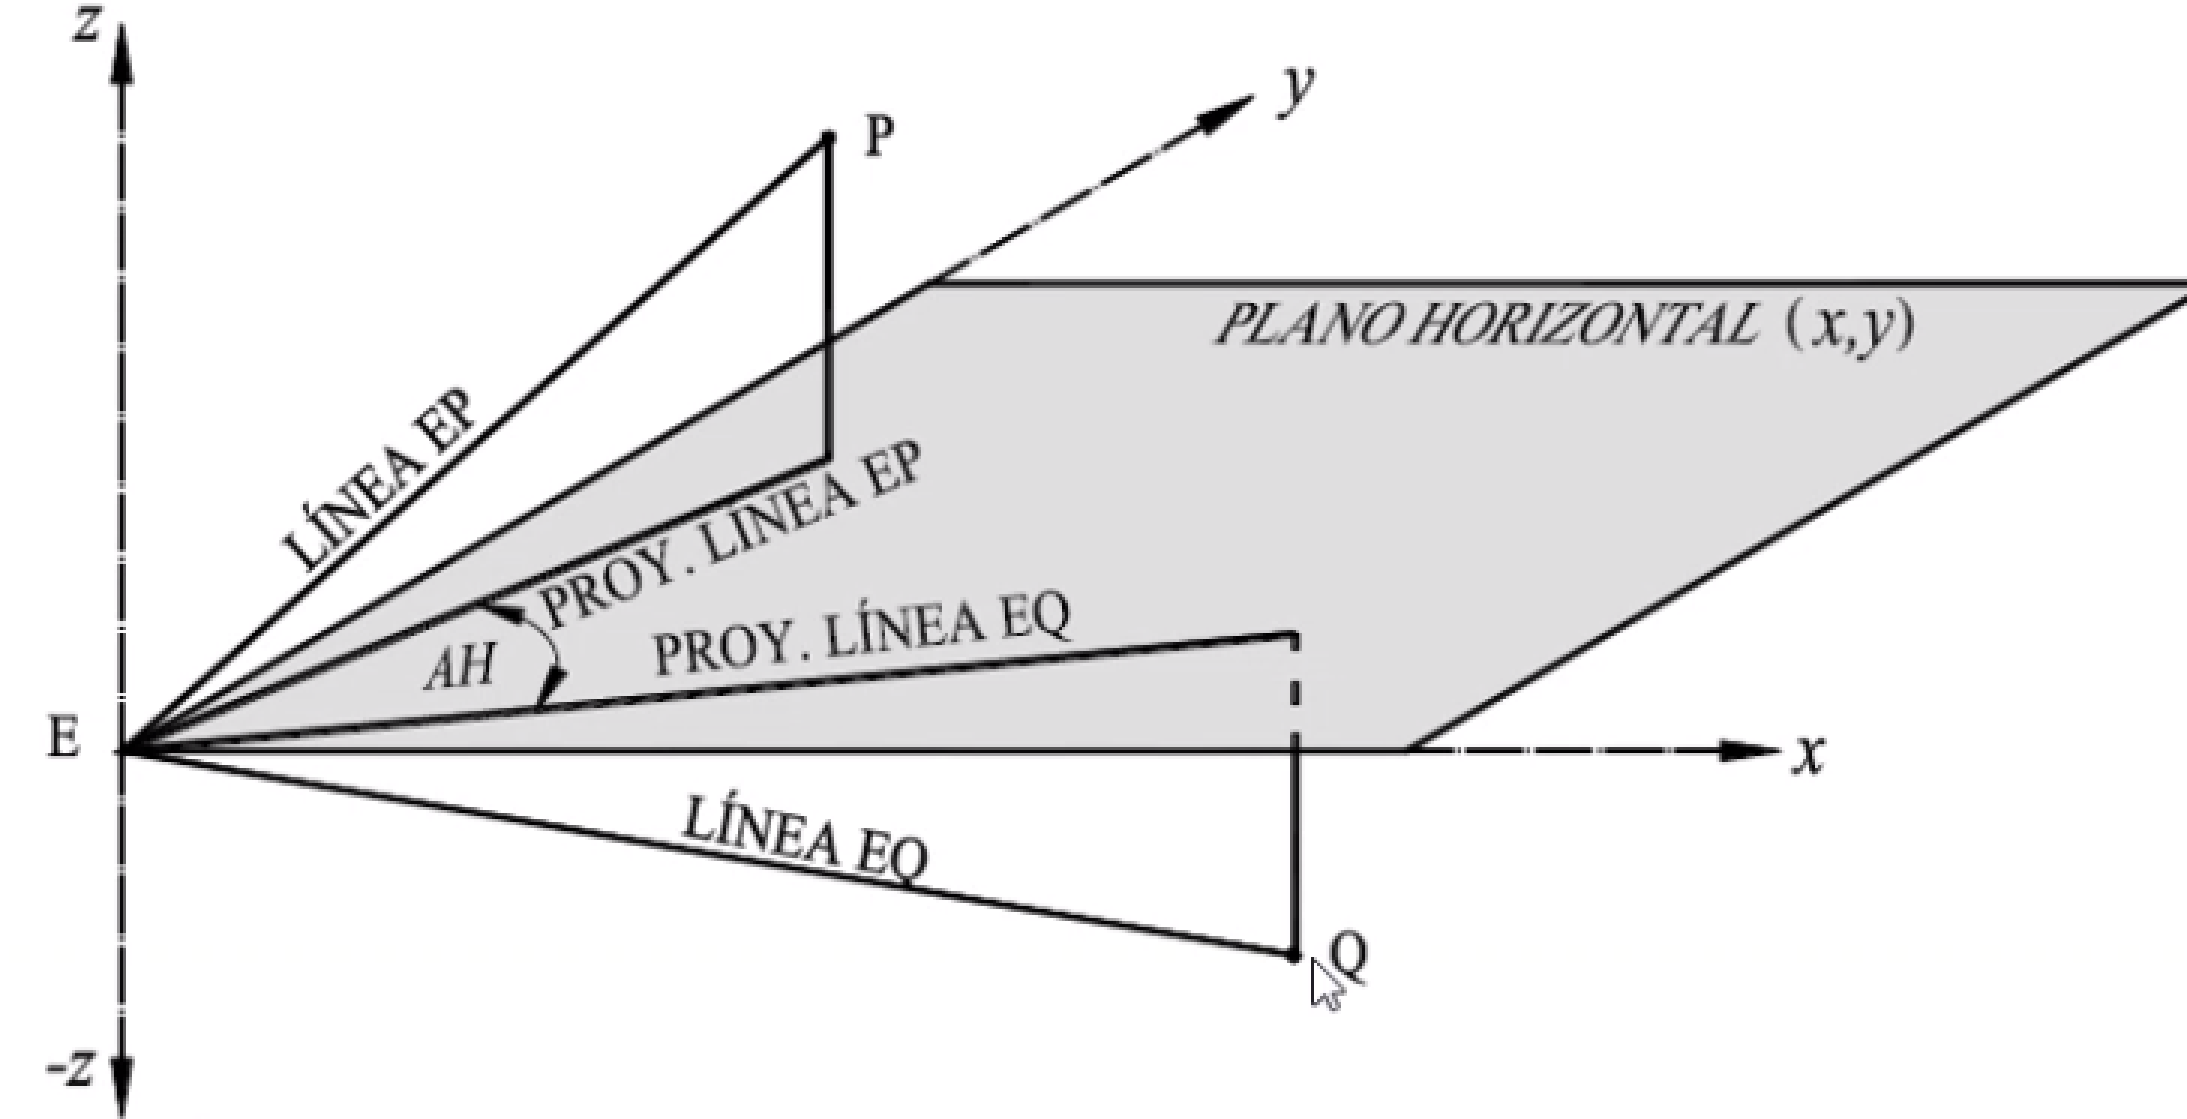
\includegraphics[width=0.5\textwidth]{ta1.png}
  \caption{Se ocupa para definir la orientación de líneas en el plano horizontal}
  \label{ta1}
\end{figure}

\subsubsection{Medición de ángulos}

\begin{definition}[Ángulo vertical]
    Es el que se genera entre las proyecciones sobre un plano vertical de dos líneas cualesquiera o de las visuales a dos puntos cualesquiera desde uno común y se mide ordinariamente en el limbo o círculo vertical del tránsito, teodolito o estación total
\end{definition}

\subsubsection{Rumbo y azimut de una línea}

\begin{definition}[Rumbo]
    El rumbo de una línea que denotaremos por la letra $R$ es el ángulo horizontal que se forma entre ésta y el meridiano que pasa por el punto en el cual se hace la medición; se mide a partir del sentido norte de la meridiana y hacia el este o hacia el oeste según la línea se localice en el cuadrante topográfico NE o en NW, respectivamente y a partir del sentido SUr y hacia el Este o hacia el Oeste también si la línea queda ubicada en el cuadrante topográfico SE o en el cuadrante SW respectivamente
\end{definition}

\begin{figure}[h!]
    \centering
    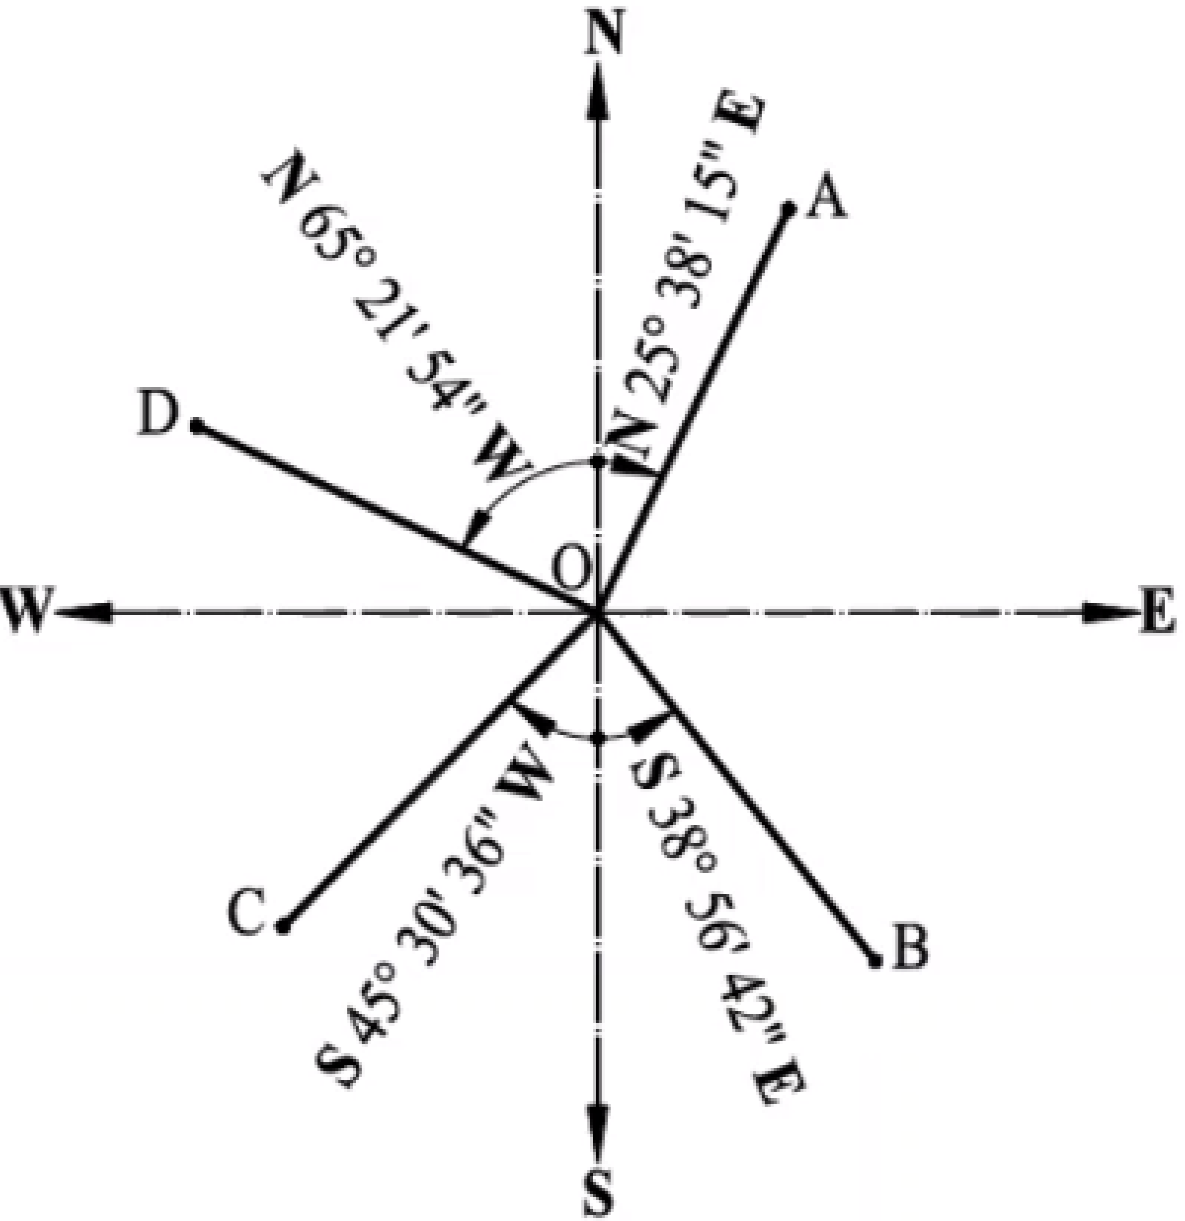
\includegraphics[width=0.5\textwidth]{ta2.png}
    \caption{Rumbo}
    \label{ta2}
\end{figure}

  \begin{definition}[Azimut]
    Es el ángulo horizontal comprendido entre ésta y el sentido Norte de la meridiana que pasa por el origen de dicha línea; se mide a partir del Norte  en el sentido horario, oscila entre $0^{\circ}$ y $360^{\circ}$
\end{definition}

Es independiente de la ubicación de la línea en los cuadrantes topográficos, lo cual hace a este parámetro de uso más fácil, común y conveniente, como se verá más adelante.

\begin{figure}[h!]
    \centering
    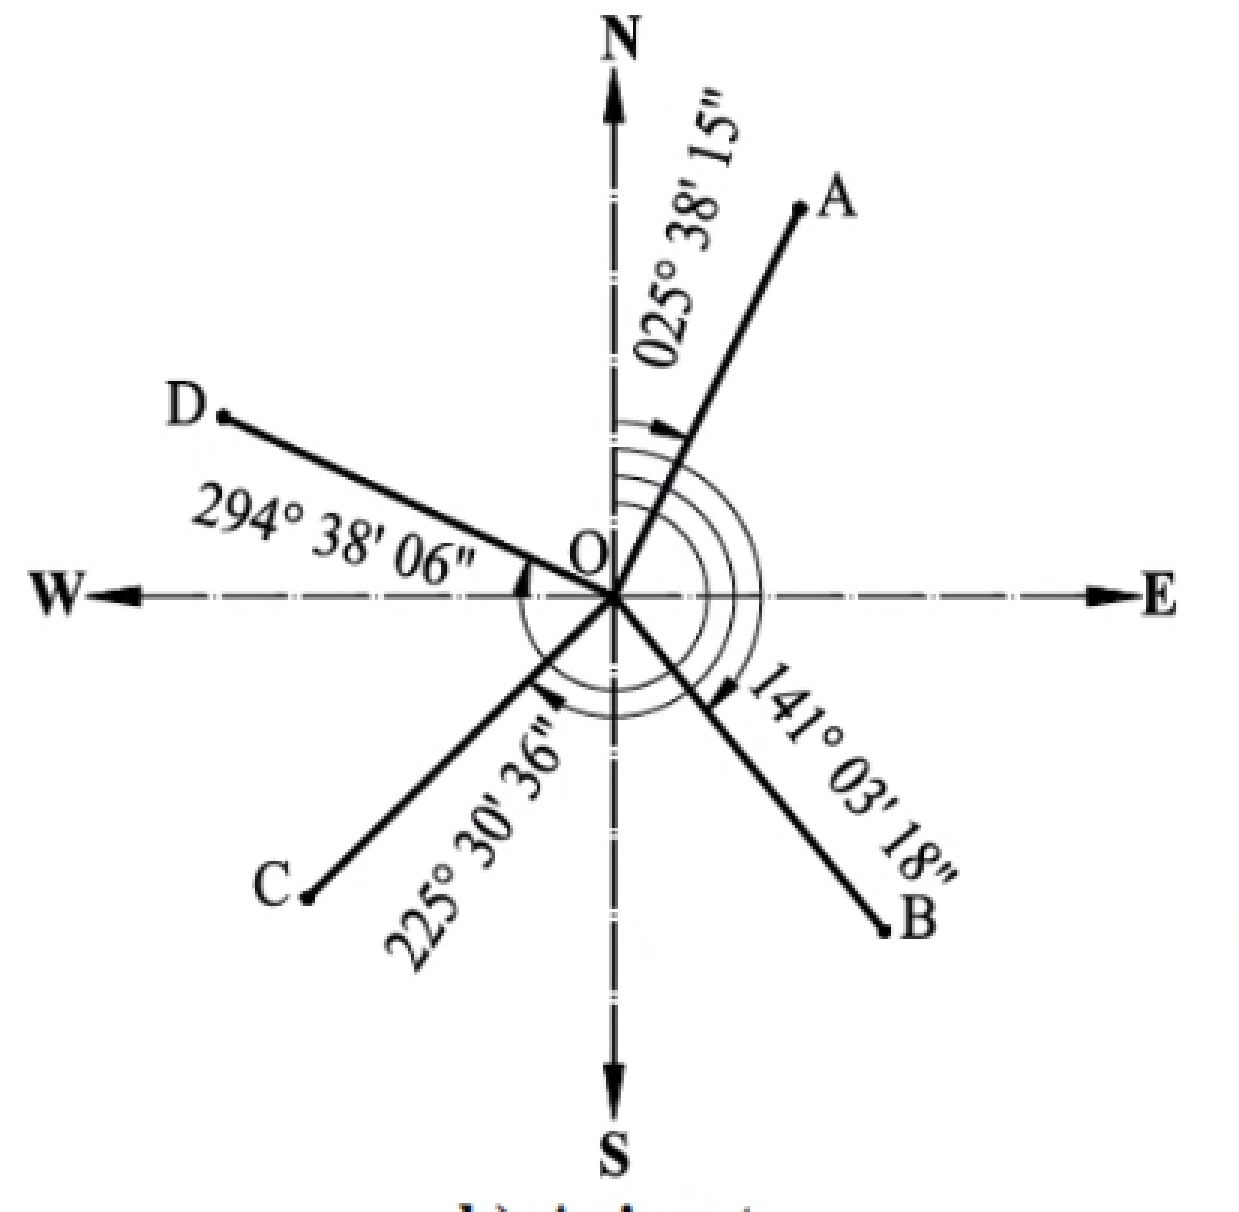
\includegraphics[width=0.5\textwidth]{ta3.png}
    \caption{Azimut}
    \label{ta3}
  \end{figure}

\begin{align}
    \text{En el cuadrante NE}&&Az=R\\ 
    \text{En el cuadrante SE}&&Az=180^{\circ}-R\\ 
    \text{En el cuadrante SW}&&Az=180^{\circ}+R\\ 
    \text{En el cuadrante NW}&&Az=360^{\circ}-R 
\end{align}

\begin{table}[h!]
    \centering
    \begin{tabular}{@{}lllll@{}}
        \toprule
        Línea & \multicolumn{2}{l}{Rumbo $(R)$}                        & \multicolumn{2}{l}{Azimut $(Az)$}                      \\ \midrule
        OA    & $R_{OA}$= & $N25^{\circ}38^{\prime}15^{\prime\prime}E$ & $Az_{OA}$= & $N25^{\circ}38^{\prime}15^{\prime\prime}$ \\
        OB    & $R_{OB}$= & $S38^{\circ}56^{\prime}42^{\prime\prime}E$ & $Az_{OB}$= & $141^{\circ}03^{\prime}18^{\prime\prime}$ \\
        OC    & $R_{OC}$= & $S45^{\circ}30^{\prime}36^{\prime\prime}W$ & $Az_{OC}$= & $225^{\circ}30^{\prime}36^{\prime\prime}$ \\
        OD    & $R_{OB}$= & $N65^{\circ}12^{\prime}54^{\prime\prime}W$ & $Az_{OB}$= & $294^{\circ}38^{\prime}06^{\prime\prime}$ \\ \bottomrule
    \end{tabular}
    \caption{Rumbo y azimut de una línea}
    \label{tabta1}
\end{table}

\begin{definition}[Ángulo vertical]
    Se forma entre ésta y el plano horizontal que pasa por el punto de inicio de la línea; se mide a partir del plano horizontal y hacia el zenit $Z$ que corresponde con el sentido positivo del eje $z$ del sistema rectangular tridimensional cuando la línea se ubica hacia arriba del plano horizontal, en cuyo caso se considera positivo; o hacia el \texttt{nadir}, que corresponde con el sentido negativo del eje z, cuando la línea se ubica hacia abajo del plano horizontal y se considera negativo.
\end{definition}

\begin{figure}[h!]
  \centerline{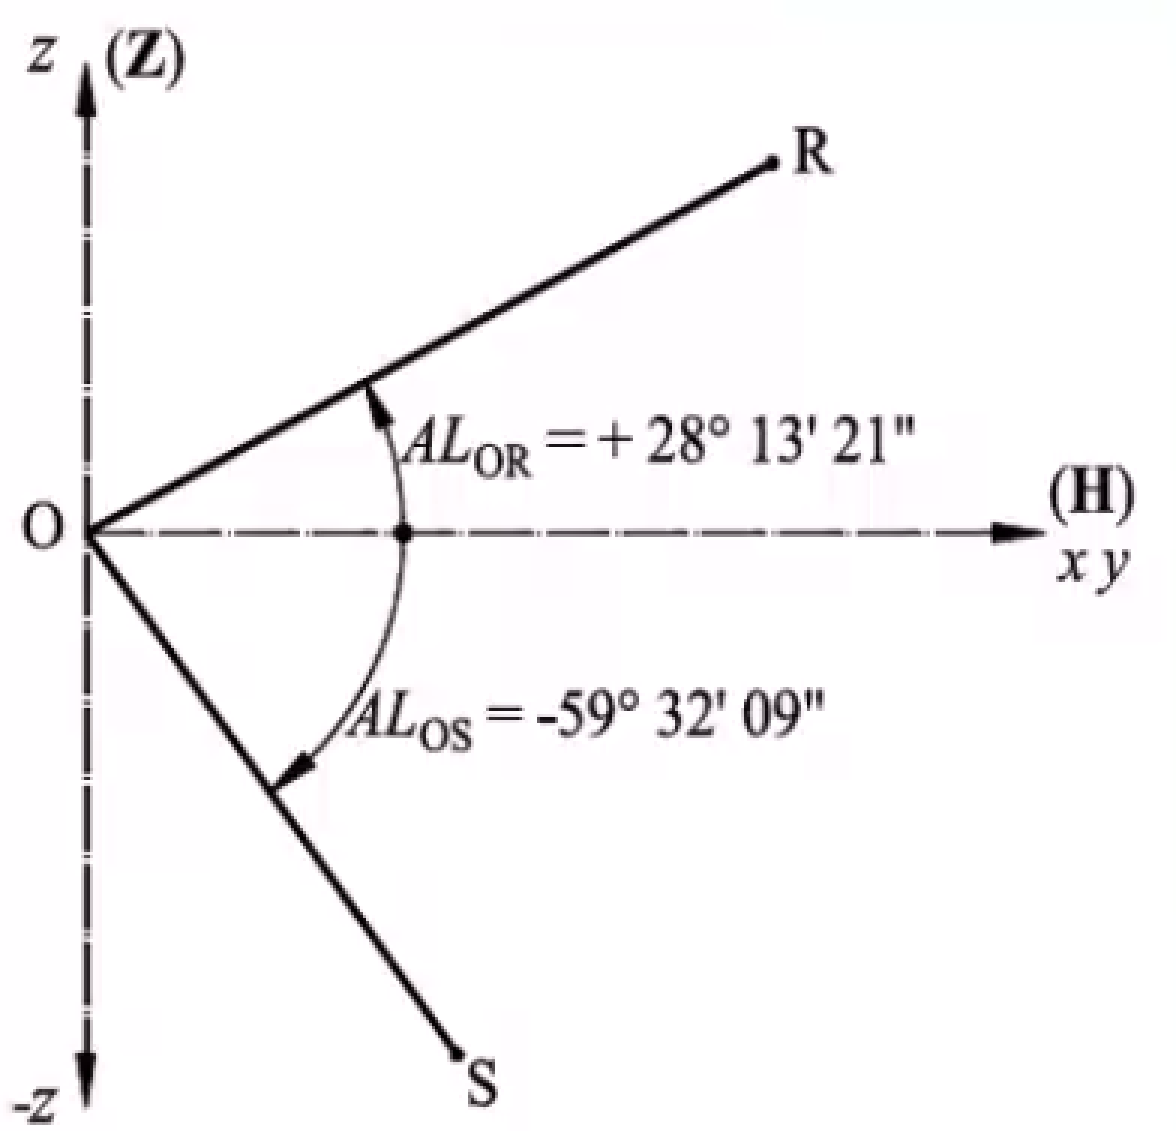
\includegraphics[width=0.5\textwidth]{ta4.png}}
  \caption{$AL=$Altura}
  \label{ta4}
\end{figure}
\subsubsection{Localización del tramo muerto}
\begin{enumerate}
    \item Existe agua suficiente para regar toda la superficie; en cuyo caso el trazo se inicia en la Obra de Toma de la Presa y se debe llegar a la parte más alta de la zona de riego para dominarla completamente.
    \item Existe mayor superficie que la que puede regarse con el volumen disponible. En este caso, el canal puede llegar a la zona de riego con una elevación con la cual se domina exclusivamente la parte más baja o con los suelos con las mejores características de productividad de la Zona Agrícola que se pretende incorporar al riego.
\end{enumerate}

DIFIERE EN DOS ASPECTOS:
\begin{enumerate}
    \item Dada su función de abastecimiento a los Canales Laterales, es recomendable mantener el nivel del agua por arriba del nivel del terreno natural, para mantener suficiente carga en los laterales para derivar hacia los sublaterales.
    \item La localización y trazo se hace sobre los planos de la ZR. recomendándose, conservar para todos los casos, altura para dominar la mayor superficie potable.
    \item 
\end{enumerate}

Diferencias de altura (h), entre el nivel del tirante normal y el nivel del terreno natural, según la superficie dominada (Sd)
\begin{equation}
    DH = \frac{Pz}{Ep \times Pg}
\end{equation}

\begin{table}[h!]
\centering
    \begin{tabular}{@{}cc@{}}
    \toprule
    SD (ha)        & h(m)                                                                                    \\ \midrule
    >100,000       & 1.50                                                                                    \\
    60,000-100,000 & 1.25                                                                                    \\
    20,000-60,000  & 1.00                                                                                    \\
    5,000-20,000   & 0.75                                                                                    \\
    <5,000         & \begin{tabular}[c]{@{}c@{}}Seguir recomendaciones\\ para canales laterales\end{tabular} \\ \bottomrule
    \end{tabular}
    \caption{La DH así obtenida, se mide entre cada par consecutivo de curvas de nivel con un compás.}
    \label{tabta22}
\end{table}
\subsubsection{De acuerdo a la Topografía}

TRES CRITERIOS:

\begin{enumerate}
    \item De acuerdo a la topografía,
    \item Siguiendo la cuadrícula y,
    \item Respetando los linderos existentes
\end{enumerate}
O alguna combinación conveniente de ellos.

Este criterio es seguramente el más económico, pues los canales laterales se localizan por los parteaguas y van abasteciendo a los sublaterales localizados hacia ambas márgenes, por lo cual la red de distribución resulta más corta que con cualquiera de los otros criterios, considerados de manera individual.

El número de estructuras de operación y de cruce resulta también menor y pueden aprovecharse los cauces y las cañadas para alojar a los drenes.

Sus principales inconvenientes son que resultan lotes irregulares y que los canales laterales y ramales tendrán pendientes mayores que la pendiente gobernadora y, por tanto, será necesario construir estructuras de control del flujo.

\subsubsection{Siguiendo la cuadrícula}

Es conveniente usar este criterio en terrenos vírgenes de gran extensión, de topografía muy plana y de poca pendiente donde el levantamiento se efectuó por el PTP de Cuadrícula Rectangular, pues se facilita su trazo en el campo y se obtienen lotes de formas regulares de las superficies que se autoricen.

La principal ventaja al usar este criterio, es que tanto la red de canales, como la de caminos y drenes, quedan ubicados sistemáticamente, y que se facilita las labores posteriores de operación y la conservación:

Se tiene como inconvenientes que la red de distribución resulta más larga que en el caso anterior, que se aumenta el número de tomas y estructuras de operación al sólo poder derivarse hacia una margen, que se requiere la construcción alternada de un canal y un dren y conduce a un incremento del número de estructuras para cruzar drenes y caminos.
\subsubsection{Respetando los linderos existentes}
Cuando la zona agrícola ya está en explotación, es decir que el parcelamiento está definido y los caminos están construidos y en operación, el criterio más apropiado es el de respetar los linderos existentes, para evitar trastornos en el régimen de la propiedad; sin embargo, a menudo los Canales deben cruzar por las parcelas cuando la pendiente de los linderos no es la requerida y, sobre todo cuando tienen pendientes positivas.

La magnitud de la red, el número de estructuras de operación y de cruce y el costo de la red resultante es muy variable cuando se sigue este criterio, ya que depende la forma de los predios y de la configuración y pendientes del terreno.

\subsection{Cálculo de curvas horizontales}

Lo ideal y conveniente desde todos los puntos de vista, es que el trazo de Vías de Comunicación sea recto y a nivel desde su origen hasta su final.

Los accidentes topográficos y los puntos obligados obligan a cambiar de dirección.

Curvas Horizontales (CH), son aquellas que se emplean en el trazo de Vías de Comunicación para suavizar los cambios de dirección y por sencillez y conveniencia en el trazo, construcción y operación, se usan arcos de circunferencia.

CURVAS DE ENLACE

Se clasifican en Simples y

Compuestas y estas últimas, a su vez, en directas e inversas

\subsubsection{Horizontales Simples}

(CHS) están constituidas por un solo tramo de circunferencia y las CH compuestas se conforman por dos curvas simples que se enlazan de manera continuada (la segunda inicia donde termina la primera) de modo que tienen una tangente común en el punto de enlace

Se denominan directas si el cambio es en el mismo sentido; en tanto que las CH compuestas inversas implican que la segunda cambia la dirección de la vía de comunicación en sentido contrario que la primera
\begin{figure}[h!]
\centering
  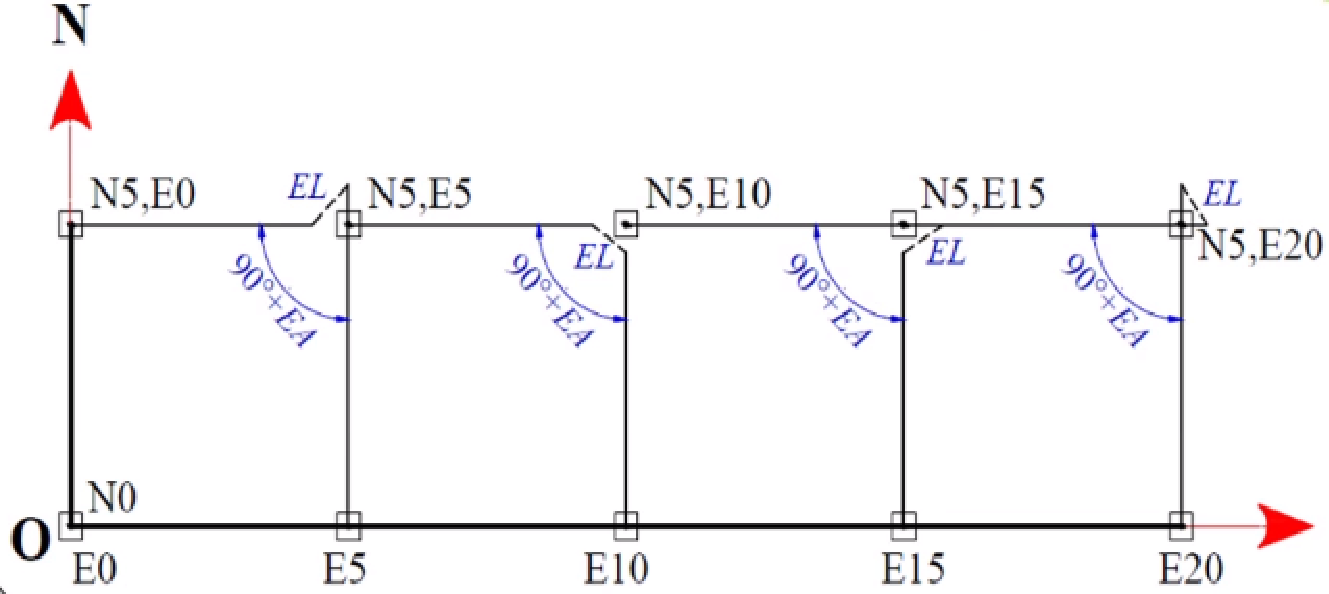
\includegraphics[width=0.5\textwidth]{ta51.pdf}
  \caption{Definición y clasificación en Curvas horizontales simples.}
  \label{ta61}
\end{figure}
Para suavizar los cambios de pendiente de las vías de comunicación como caminos y vías férreas, es decir, en el plano vertical, se l emplean las Curvas Verticales (CV), que unen dos pendientes P sucesivas y que de ordinario son arcos de parábola
\begin{figure}[h!]
\centering
  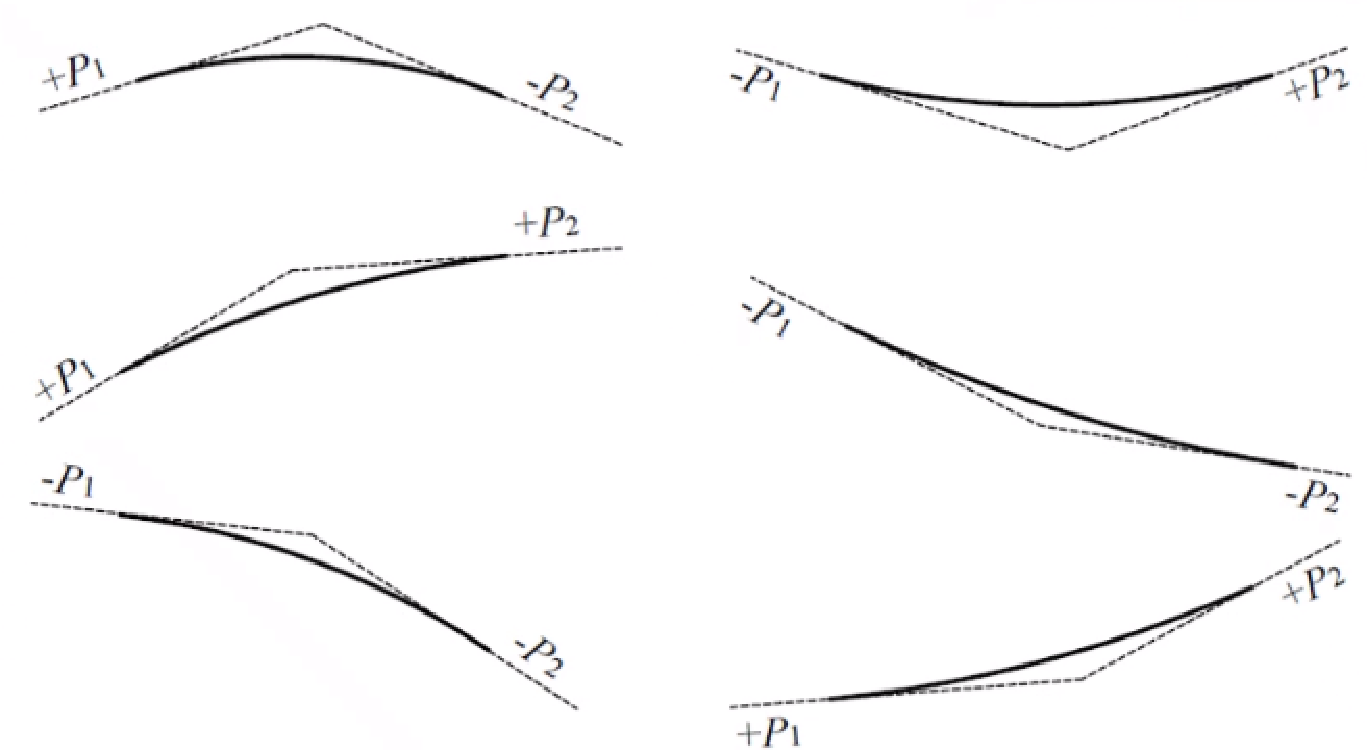
\includegraphics[width=0.5\textwidth]{ta62.pdf}
  \caption{Columpios}
  \label{ta62}
\end{figure}

$\Delta=$ \textbf{Deflexión}. Ángulo formado por la prolongación de la LCA que se constituye en tangente de entrada y la LCA que es tangente de salida y que corresponde con el cambio de dirección del trazo de la Vía de Comunicación.

$PI=$ \textbf{Punto de intersección o de inflexión}. Es el PCA o vértice en que se cruzan las tangentes de entrada y de salida y donde se mide el cambio de dirección del trazo mediante el Ángulos de Deflexión.

$ST=$ \textbf{Subtangente}. Es el tramo idéntico de las agentes de entrada (del punto de Principio de Curva PC al Punto de Intersección PI) y de salida (del PI al Punto de Término de Curva PT), entre los que se extiende la curva.

$PC=$ \textbf{Principio de Curva}. Punto común entre la tangente de entrada y la curva y en el que inicia la curva en el sentido del trazo.

$PT=$ \textbf{Principio de Tangente}. Es el punto común entre la tangente de salida y la curva, por lo que también se conoce como punto de término de la curva.

$O$ \textbf{Centro de curvatura}. Se obtiene por la intersección de las perpendiculares a la tangente de entrada en el PC y a la tangente de salida en el PT y se constituyen en el radio de la curva.

$R=$ \textbf{Radio de curvatura.} Distancia del centro de curvatura O a cualquiera de los puntos de la curva.

$C=$ \textbf{Cuerda.} Es la longitud de los tramos rectos con los que se traza la curva al unir puntos consecutivos sobre ella; su valor generalmente es de 20 m.

$CP=$ \textbf{Cuerda principal}. Es la cuerda subtendida por la curva desde el PC hasta el PT.

$G=$ \textbf{Grado de curvatura.} Es el ángulo central, es decir, que se mide en el centro de curvatura, que subtiende a la cuerda C que se utiliza en el trazo de la curva.

$LC=$ \textbf{Longitud de curva.} Es la longitud de la curva obtenida como la suma de las cuerdas C.

$SC=$ \textbf{Subcuerda.} Es la magnitud de una cuerda de menor longitud que

$G^{\prime}=$ \textbf{Subgrado}. Es el ángulo central (medido en el centro de curvatura O), que subtiende una Subcuerda SC.

\begin{figure}[h!]
\centering
  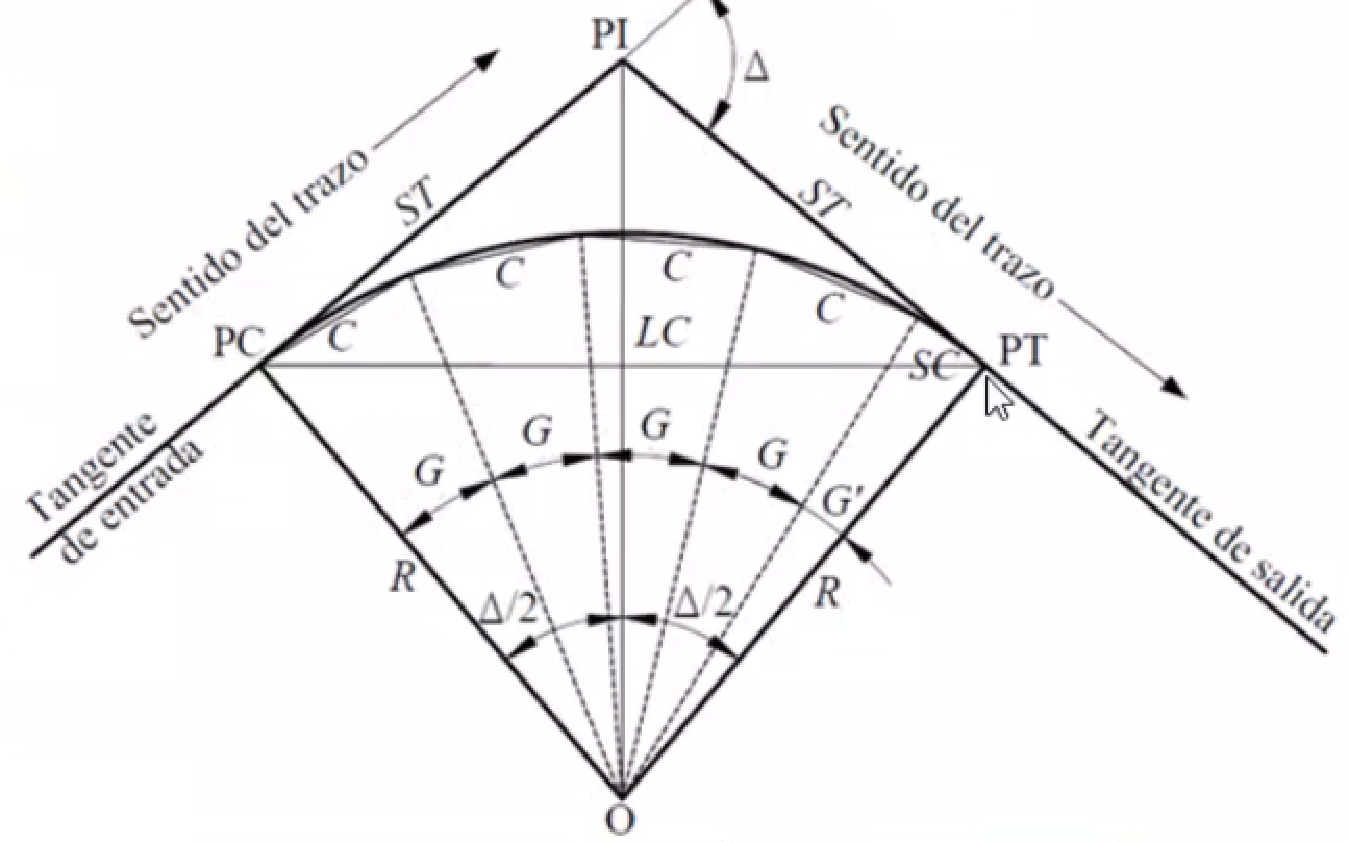
\includegraphics[width=0.5\textwidth]{ta63.pdf}
  \caption{Elementos de una CHS.}
  \label{ta63}
\end{figure}

\textbf{A.} Se mide directamente en campo con el trazo de la Poligonal de Apoyo, o bien se obtiene de los datos del proyecto en caso de replantear el trazo del eje de la vía en los planos.

\textbf{C.} Su valor está estrechamente relacionado. con G y R, evidentemente, para un radio fijo, mayores valores de G producen mayores valores de C

Se recomienda:
\begin{itemize}
    \item $C=20$ m para $G < 10^{\circ} \implies R > 100 m$
    \item $10^{\circ} <G<20^{\circ}$ se usan cuerdas de 10 m
    \item $20<G<40$ se usan cuerdas de 5m.
\end{itemize}

\textbf{R.} Se debe tratar de que sea lo mayor posible para no tener curvas forzadas, pero adaptándose lo mejor que se pueda a la configuración del terreno para no producir terracerías costosas

Generalmente se toma un mínimo de R = 35 m (que equivale aproximadamente a G = $35^{\circ}$) aun para caminos de segundo orden, pero se prefiere que R sea mayor 100 m.

En Canales, los radios dependen de muchos factores, entre los que destacan la velocidad, la pendiente, el tirante, el ancho total del canal, pero no hay limitaciones generales, pudiendo considerarse como mínimo, un valor de R del doble al triple del ancho total del canal.

\textbf{Cad Pl.} Se obtiene de las mediciones lineales al trazar la Poligonal de Apoyo.

\begin{figure}[h!]
\centering
  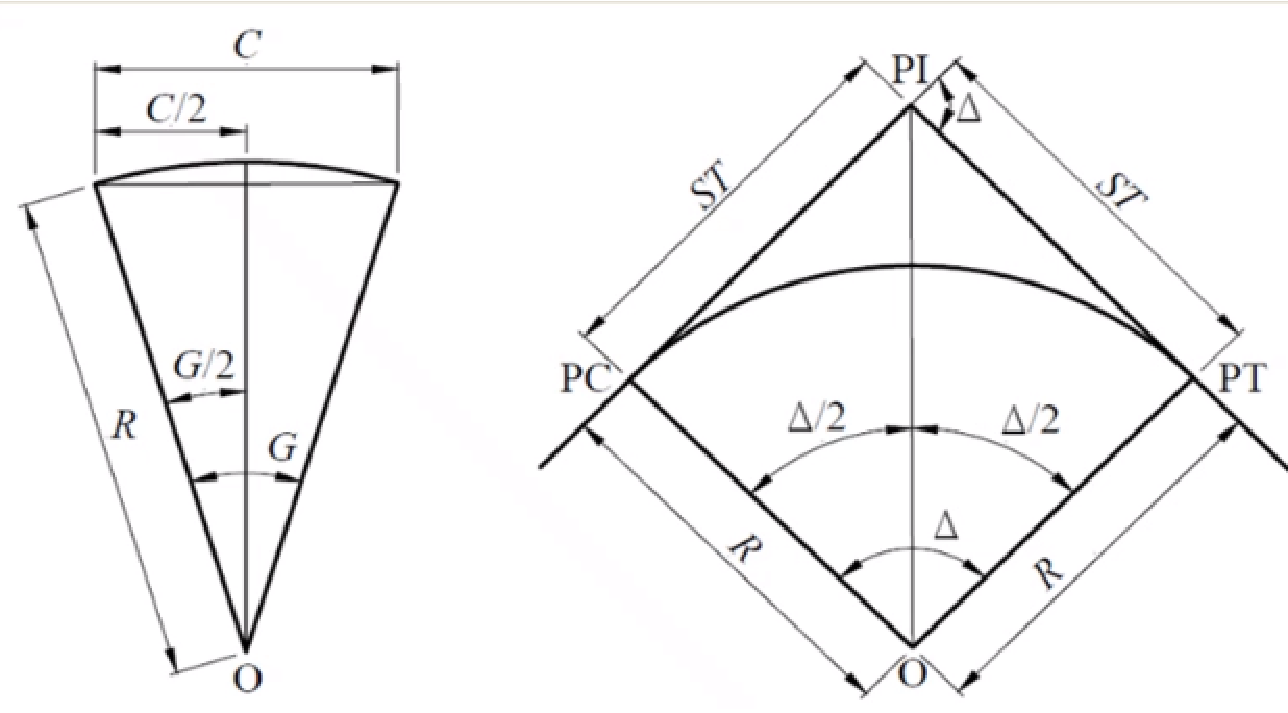
\includegraphics[width=0.5\textwidth]{ta64.pdf}
  \caption{Procedimiento de cálculo de una CHS}
  \label{ta64}
\end{figure}
Radio de curvatura:
\begin{align}
    &\sin{\left(\frac{G}{2}\right)}=\frac{\frac{C}{2}}{R}& R = \frac{\frac{C}{2}}{\sin{\left(\frac{G}{2}\right)}}\\
    &C = 20m&R = \frac{10}{\sin{\left(\frac{G}{2}\right)}}\\
\end{align}
Subtangente:
\begin{align}
    &\tan{\frac{\Delta}{2}} = \frac{ST}{R}\\
    &ST = R \times \tan{\frac{\Delta}{2}}  
\end{align}
Longitud de curva:
\begin{equation*}
    LC = C\left(\frac{\Delta}{G}\right)\, si\, C= 20\implies LC = 20\left(\frac{\Delta}{G}\right)
\end{equation*}
Cadenamientos del PC y del PT
\begin{align}
    &CadPC = CadPI - ST\\
    &CadPT = CadPI + LC
\end{align}
Subcuerdas de Entrada y Salida
\begin{align}
    &SCe = PCC - CadPC\\
    &SCs = CadPT - UCC
\end{align}
\begin{figure}[h!]
\centering
  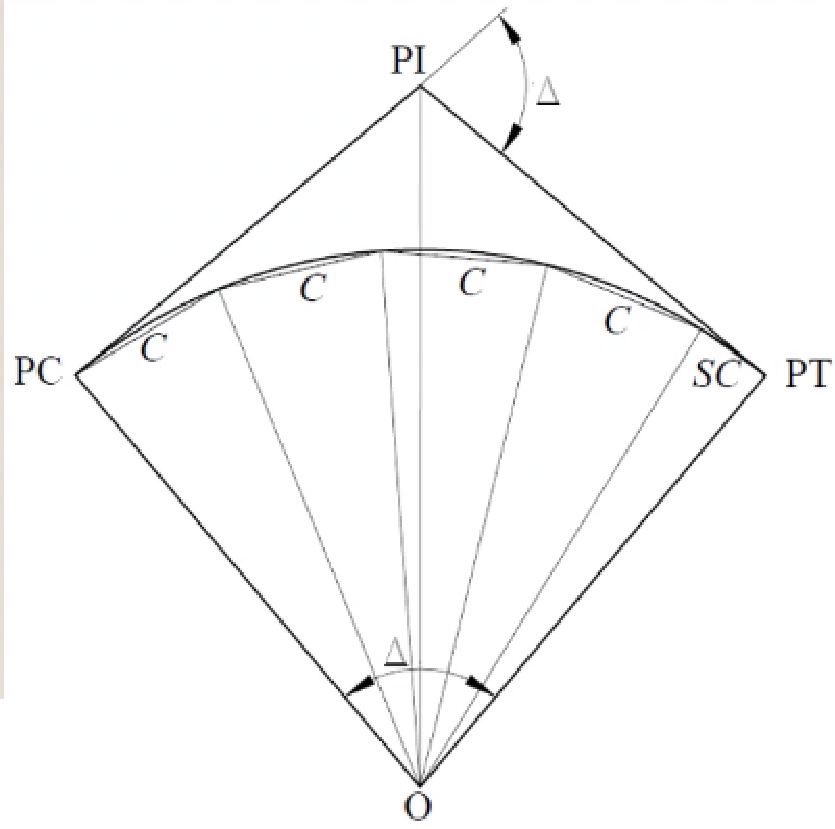
\includegraphics[width=0.5\textwidth]{ta65.pdf}
  \caption{Procedimiento de cálculo de una CHS}
  \label{ta65}
\end{figure}
\subsubsection{Cálculo de una CHS para su trazo por el MÉTODO DE DEFLEXIONES}

El método se basa en la siguiente propiedad geométrica de las CHS: Cualquier cuerda que es subtendida con un ángulo a desde el centro de curvatura O, se subtenderá con un ángulo $\alpha/2$ desde el PC

Se puede trazar un punto cualquiera sobre la curva, a partir de uno anterior, midiendo una cuerda M desde el punto anterior y un ángulo 8 (con vértice en el PC), también desde el punto anterior de la curva, de tal forma que $\delta =\alpha/2$ el ángulo central que subtiende a la cuerda M
\begin{equation*}
    Si\, C = 20 m:\implies \delta c  \frac{G}{2}
\end{equation*}
Para trazar el primer punto sobre la curva ($PCC$) y el último punto sobre la curva ($PT$), se usan las subcuerdas de entrada ($SCe$) y de salida ($SCs$) y la Deflexión de Entrada de y Deflexión de Salida $\delta s$,
\begin{align}
    &\delta e = \delta \times SCe\\
    &\delta s = \delta \times SCs\\
    &\delta = \frac{\frac{G}{2}}{20}= \frac{G}{40}
\end{align}

\begin{example}
    Datos: $\Delta= 26^{\circ}30^{\prime}$, $G=4^{\circ}$ que implica $C=20m$ y CadPI=8+122.350
\end{example}
\textit{ Sol. }

\begin{enumerate}
    \item Cálculo de Radio de curvatura $R$:
    \begin{equation*}
        R = \frac{\frac{20}{2}}{\sin{\frac{4}{2}}}= \frac{10}{\sin{2^{\circ}}} = 286.537m
    \end{equation*}
    \item Cálculo de la subtangente ST:
    \begin{equation*}
        ST = 286.537\times \tan{\frac{26^{\circ}30^{\prime}}{2}} = 67.471
    \end{equation*}
    \item Cálculo de la longitud de Curva LC:
    \begin{equation*}
        LC = 20\times \frac{26^{\circ}30^{\prime}}{4^{\circ}} = 132.500m
    \end{equation*}
    \item Cálculo del cadenamiento del PC y del PT
    \begin{align*}
        CadPC = 8 +122.350 - 64.471 = 8 + 057.879\\
        CadPT = 8 + 057.879 + 132.500 = 8 + 190.379
    \end{align*}
    \item Cálculo de las subcuerdas
    \begin{align*}
        &SCe = 8 + 060 +8 + 057.878 = 2.121m\\
        &SCs = 8 + 190.379-8 + 180 = 10.379m
    \end{align*}
    \item Cálculo de la deflexión por cuerda $\delta c$
    \begin{equation*}
        \delta c = \frac{4^{\circ}}{2} = 2^{\circ} 
    \end{equation*}
    \item Cálculo de las deflexiones unitaria $\delta$ de entrada $\delta e$ y de salida $\delta s$:
    \begin{align*}
        &\delta = \frac{4}{40} = 0^{\circ}06^{\prime}00^{\prime\prime}m\\
        &\delta e= 6^{\prime} \times 2.121 = 2.726^{\prime} = 00^{\circ}12^{\prime}3.56^{\prime\prime}m\\
        &\delta s= 6^{\prime} \times 10.379 = 62.274^{\prime} = 01^{\circ} 2^{\prime} 64^{\prime\prime}m
    \end{align*}
\end{enumerate}

\begin{table}[h!]
    \centering
    \begin{tabular}{@{}ccccccccc@{}}
    \toprule
    \multirow{3}{*}{EST.} & \multirow{3}{*}{P.V.} & \multirow{2}{*}{\begin{tabular}[c]{@{}c@{}}Cuerdas\\ Parciales\end{tabular}} & \multicolumn{6}{c}{Deflexiones}                                           \\
                          &                       &                                                                              & \multicolumn{3}{c}{Parciales}       & \multicolumn{3}{c}{Acumuladas}      \\
                          &                       & (m)                                                                          & $\circ$ & $\prime$ & $\prime\prime$ & $\circ$ & $\prime$ & $\prime\prime$ \\ \midrule
    PC                    & PI                    & 0.000                                                                        & 00      & 00       & 00.00          & 00      & 00       & 00.00          \\
                          & 8+060                 & 0.000                                                                        & 00      & 00       & 00.00          & 00      & 00       & 00.00          \\
                          & 8+080                 & 2.121                                                                        & 00      & 12       & 43.56          & 02      & 12       & 43.56          \\
                          & 8+100                 & 20.000                                                                       & 02      & 00       & 00.00          & 04      & 12       & 43.56          \\
                          & 8+120                 & 20.000                                                                       & 02      & 00       & 00.00          & 06      & 12       & 43.56          \\
                          & 8+140                 & 20.000                                                                       & 02      & 00       & 00.00          & 08      & 12       & 43.56          \\
                          & 8+160                 & 20.000                                                                       & 02      & 00       & 00.00          & 10      & 12       & 43.56          \\
                          & 8+180                 & 20.000                                                                       & 02      & 00       & 00.00          & 12      & 12       & 43.56          \\
                          & 8+187.38              & 10.379                                                                       & 01      & 02       & 16.44          & 13      & 15       & 00.00          \\
                          & SUMAS                 & 132.500                                                                      & 13      & 15       & 00.00          & \multicolumn{3}{c}{=$\Delta/2$}     \\ \bottomrule
    \end{tabular}
    \caption{Sistematización de los cálculos y resultados para el trazo por el método de Deflexiones}
    \label{tabta23}
\end{table}

\subsubsection{Por el método de Deflexiones desde el PC}

Se debe contar con un Instrumento para medición de ángulos (Tránsito, Teodolito o Estación Total) y cinta métrica de longitud mayor que el de una Cuerda
\begin{enumerate}
    \item Se hace estación con el Teodolito en el PI, se visa hacia el PCA que define la tangente de entrada y se mide con cinta ST (igual a 67.471 m, para el ejemplo), con lo que se determina la ubicación del PC y se establece con un trompo y una estaca.
    \item Se da vuelta de campana al telescopio; en dicha dirección, se coloca el cero el AH y se mide en el sentido correspondiente el valor del ángulo de Deflexión $\Delta(26^{\circ} 30^{\prime})$, con lo que se obtiene la dirección de la tangente de salida.
    \item Se mide con cinta (o con el MED de la ET) una distancia igual a ST en la dirección de la tangente de salida. con lo que se determina la ubicación del PT, mismo que se establece con un trompo y correspondiente. 
    \item Se estaciona el Teodolito en el PC, se visa el PI y se pone en ceros el círculo de ángulos horizontales.
    \item Para ubicar el primer punto sobre la curva (PCC Cad. 8+060 punto 1), se mide el ángulo de $(00^{\circ} 12^{\prime} 43.56^{\prime\prime})$, en esa dirección se mide con la cinta desde el $PC$ la $SCe$ (2.121m) y se determina la ubicación del punto con trompo y estaca.
    \item El segundo punto sobre la curva (Cad. 8+080 punto 2), se ubica agregando en el círculo horizontal un valor \& $(02^{\circ}, 00^{\prime} 00^{\prime\prime})$ que equivale a medir desde la dirección al PI la deflexión acumulada ($02^{\circ} 12^{\prime} 43.56^{\prime\prime}$); en la dirección determinada se localizará el punto 2, justo en la intersección de la visual con la medida con la cinta de una Cuerda (20 m) desde el punto 1.
    \begin{figure}[h!]
    \centering
      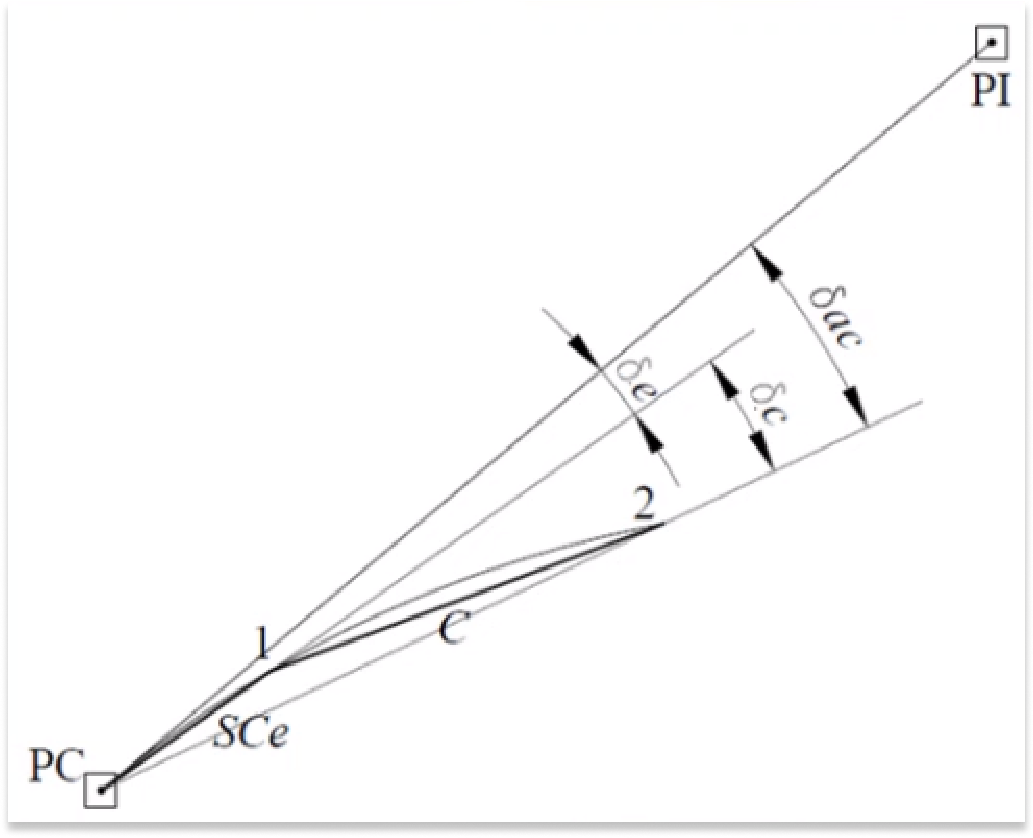
\includegraphics[width=0.5\textwidth]{ta66.pdf}
      \caption{Trazo de CHS en campo}
      \label{ta66}
    \end{figure}
    
    \item Los demás puntos sobre la curva, se ubican de manera análoga que el punto 2 (a excepción del último, que corresponde con el PT y que ya se ubicó desde el PI como se indicó en el inciso d), midiendo para la correspondiente cada uno declinación acumulada $(\Delta ac)$ y una Cuerda con cinta desde el punto anterior.
    
    El trazo de la curva se comprueba, visando el PT y midiendo el ángulo generado en el círculo vertical del teodolito (SAM= semideflexión medida); el cual se compara con la última deflexión acumulada ($\Delta/2$), con lo que se obtiene el error angular del trazo EAt
    \begin{equation*}
            EAt=S\Delta M - \frac{\Delta}{2} 
    \end{equation*}
    
    Si el valor absoluto del error no excede, emplea tránsito o de $10^{\prime\prime}$ si se emplea de $01^{\prime}$ si se emplea teodolito con aproximación de $1^{\prime\prime}$, se aceptará que el trazo angularmente
\end{enumerate}

El trazo se aceptará linealmente, si el valor absoluto de la diferencia entre la Subcuerda de Salida medida en el terreno (SCsm) y la Subcuerda de Salida calculada (SCsc), que será el Error Lineal del trazo (ELt), no excede la Tolerancia TLt
\begin{align}
    &ELt = SCsm - SCsc\\
    &TLt = 2 \sqrt{n}
\end{align}
Para el ejemplo resuelto en la sección anterior, en que n = 8, TLt = 5.657 cm.

Si alguno de los errores (angular o lineal), excede a su respectiva tolerancia, se rechaza el trabajo efectuado y debe repetirse hasta que se cumplan ambas condiciones, y si ambos errores cumplen con sus respectivas tolerancias, se deja como PT el previamente establecido.

El Punto de Inflexión PI es inaccesible, por la presencia de una zona a la que no se puede acceder con el Instrumento para hacer las mediciones necesarias para el trazo
\begin{figure}[h!]
\centering
  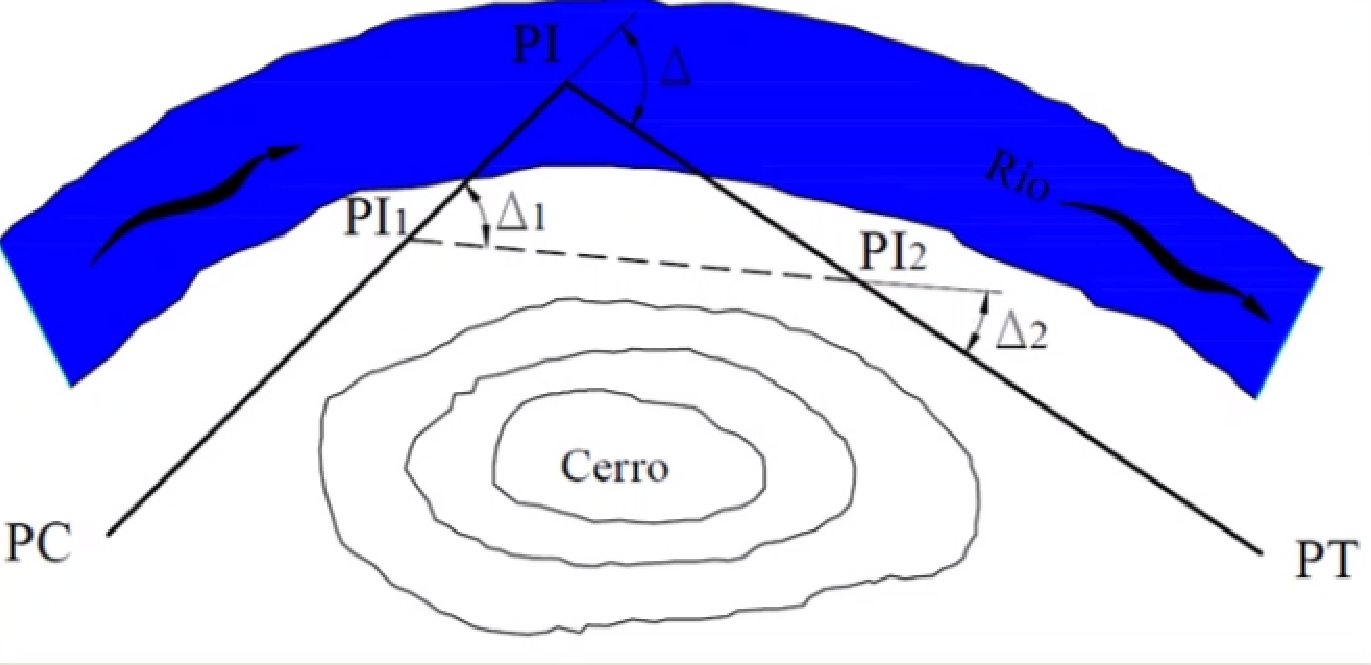
\includegraphics[width=0.5\textwidth]{ta67.pdf}
  \caption{Problema especial para el cálculo}
  \label{ta67}
\end{figure}
Aplicando la Ley de los Senos, se pueden calcular las distancias 1-PI y 2-PI y se puede obtener el cadenamiento del PI (CadPI).
\begin{align*}
    \frac{D_{12}}{\sin{180^{\circ} -\Delta}} = \frac{1 - PI}{\sin{\Delta_2}} = \frac{2 - PI}{\sin{\Delta_1}}\\
    CadPI = CadPI_1 +1 - PI
\end{align*}
Conocida la deflexión $\Delta$ y el $CadPI$, se hace el cálculo normal de la curva, corroborando que tanto el PC como el PT queden dentro del tramo "accesible", lo cual quizá requiera de hacer varios ensayos. pero finalmente, se tendrá la curva que satisfaga las restricciones ocasionadas por la inaccesibilidad del Pl.


\begin{definition}[Ángulo Zenital]
    Es el ángulo vertical que se forma entre esta y la dirección de la vertical del lugar de observación, que pasa por le punto en el cual se hace la medición; se mide a partir del sentido del zenit $Z$
\end{definition}

\begin{equation}
    AL+AZ=90^{\circ}
\end{equation}

\begin{figure}[h!]
  \centerline{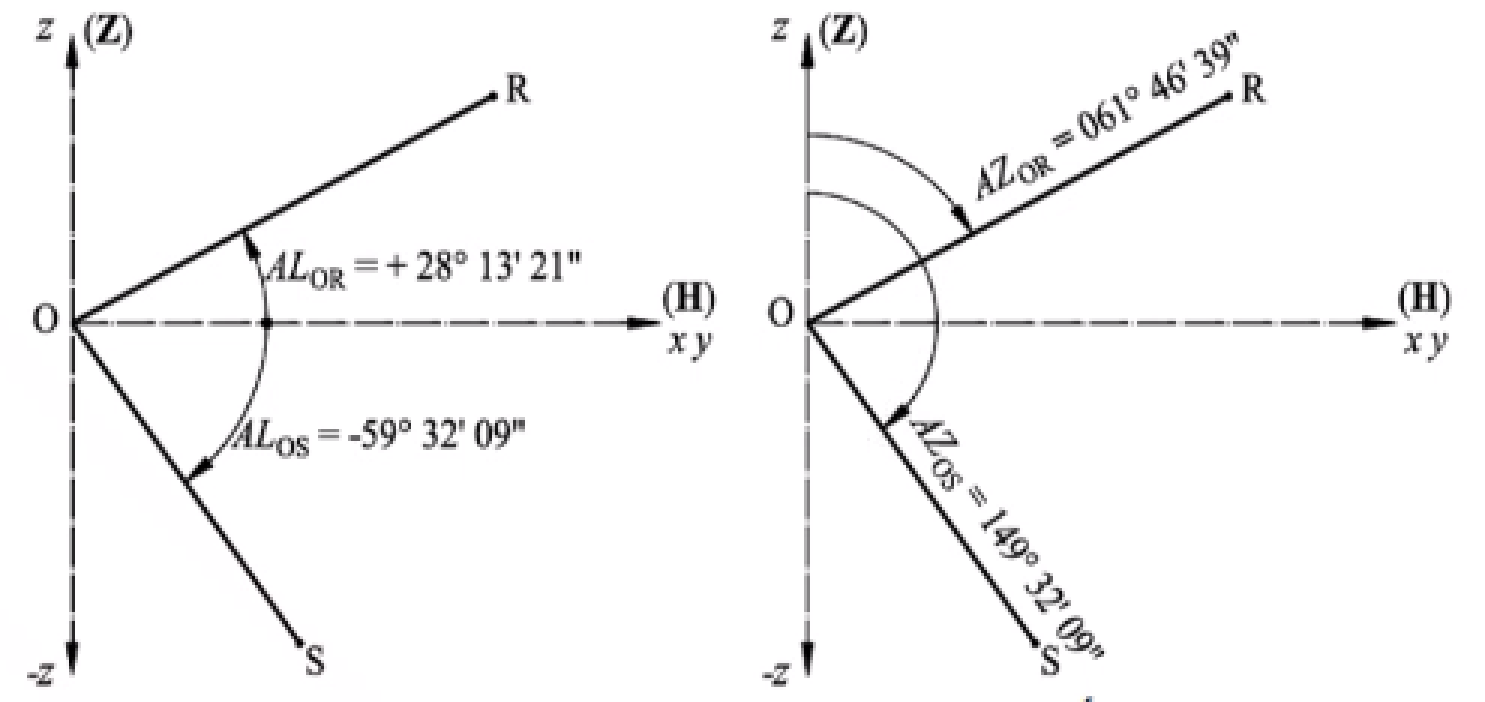
\includegraphics[width=0.5\textwidth]{ta5.png}}
  \caption{Altura y Ángulo Cenital}
  \label{ta5}
\end{figure}

\begin{table}[h!]
    \centering
    \begin{tabular}{lllll}
        \hline
        Línea & \multicolumn{2}{l}{Rumbo $(R)$}                        & \multicolumn{2}{l}{Azimut $(Az)$}                      \\ \hline
        OR    & $AL_{OR}$= & $+28^{\circ}13^{\prime}21^{\prime\prime}$ & $Az_{OA}$= & $61^{\circ}46^{\prime}39^{\prime\prime}$  \\
        OS    & $AL_{OS}$= & $-59^{\circ}32^{\prime}09^{\prime\prime}$ & $Az_{OS}$= & $149^{\circ}32^{\prime}09^{\prime\prime}$
    \end{tabular}
    \caption{Ángulos}
    \label{tabta2}
\end{table}

\begin{problem}[Completar la tabla]

    
\begin{table}[h!]
    \centering
    \begin{tabular}{@{}llllll@{}}
        \toprule
        Línea & \multicolumn{2}{l}{Rumbo $(R)$}                                & Azimut $(Az)$                             & Altura $(AL)$                              & \begin{tabular}[c]{@{}l@{}}Ángulo\\ Zenital\\ $(AZ)$\end{tabular} \\ \midrule
        JK    & \multicolumn{2}{l}{}                                           & $145^{\circ}01^{\prime}19^{\prime\prime}$ &                                            & $162^{\circ}12^{\prime}08^{\prime\prime}$                         \\
        QR    & \multicolumn{2}{l}{$N15^{\circ}29^{\prime}49^{\prime\prime}$}  &                                           & $+005^{\circ}18^{\prime}52^{\prime\prime}$ &                                                                   \\
        HT    & \multicolumn{2}{l}{}                                           & $327^{\circ}54^{\prime}35^{\prime\prime}$ & $-022^{\circ}30^{\prime}42^{\prime\prime}$ &                                                                   \\
        DS    & \multicolumn{2}{l}{$N512^{\circ}28^{\prime}42^{\prime\prime}$} &                                           &                                            & $038^{\circ}25^{\prime}46^{\prime\prime}$                         \\ \bottomrule
    \end{tabular}
    \caption{Completar los valores faltantes}
    \label{tabta3}
    \end{table}
\end{problem}

\subsubsection{Elementos de puntos}

\begin{align}
    &X_p=X_E+P_{xEP}\\ 
    &Y_p=Y_E+P_{yEP}\\Z
    &Z_p=Z_E+P_{zEP}
\end{align}

\begin{figure}[h!]
  \centerline{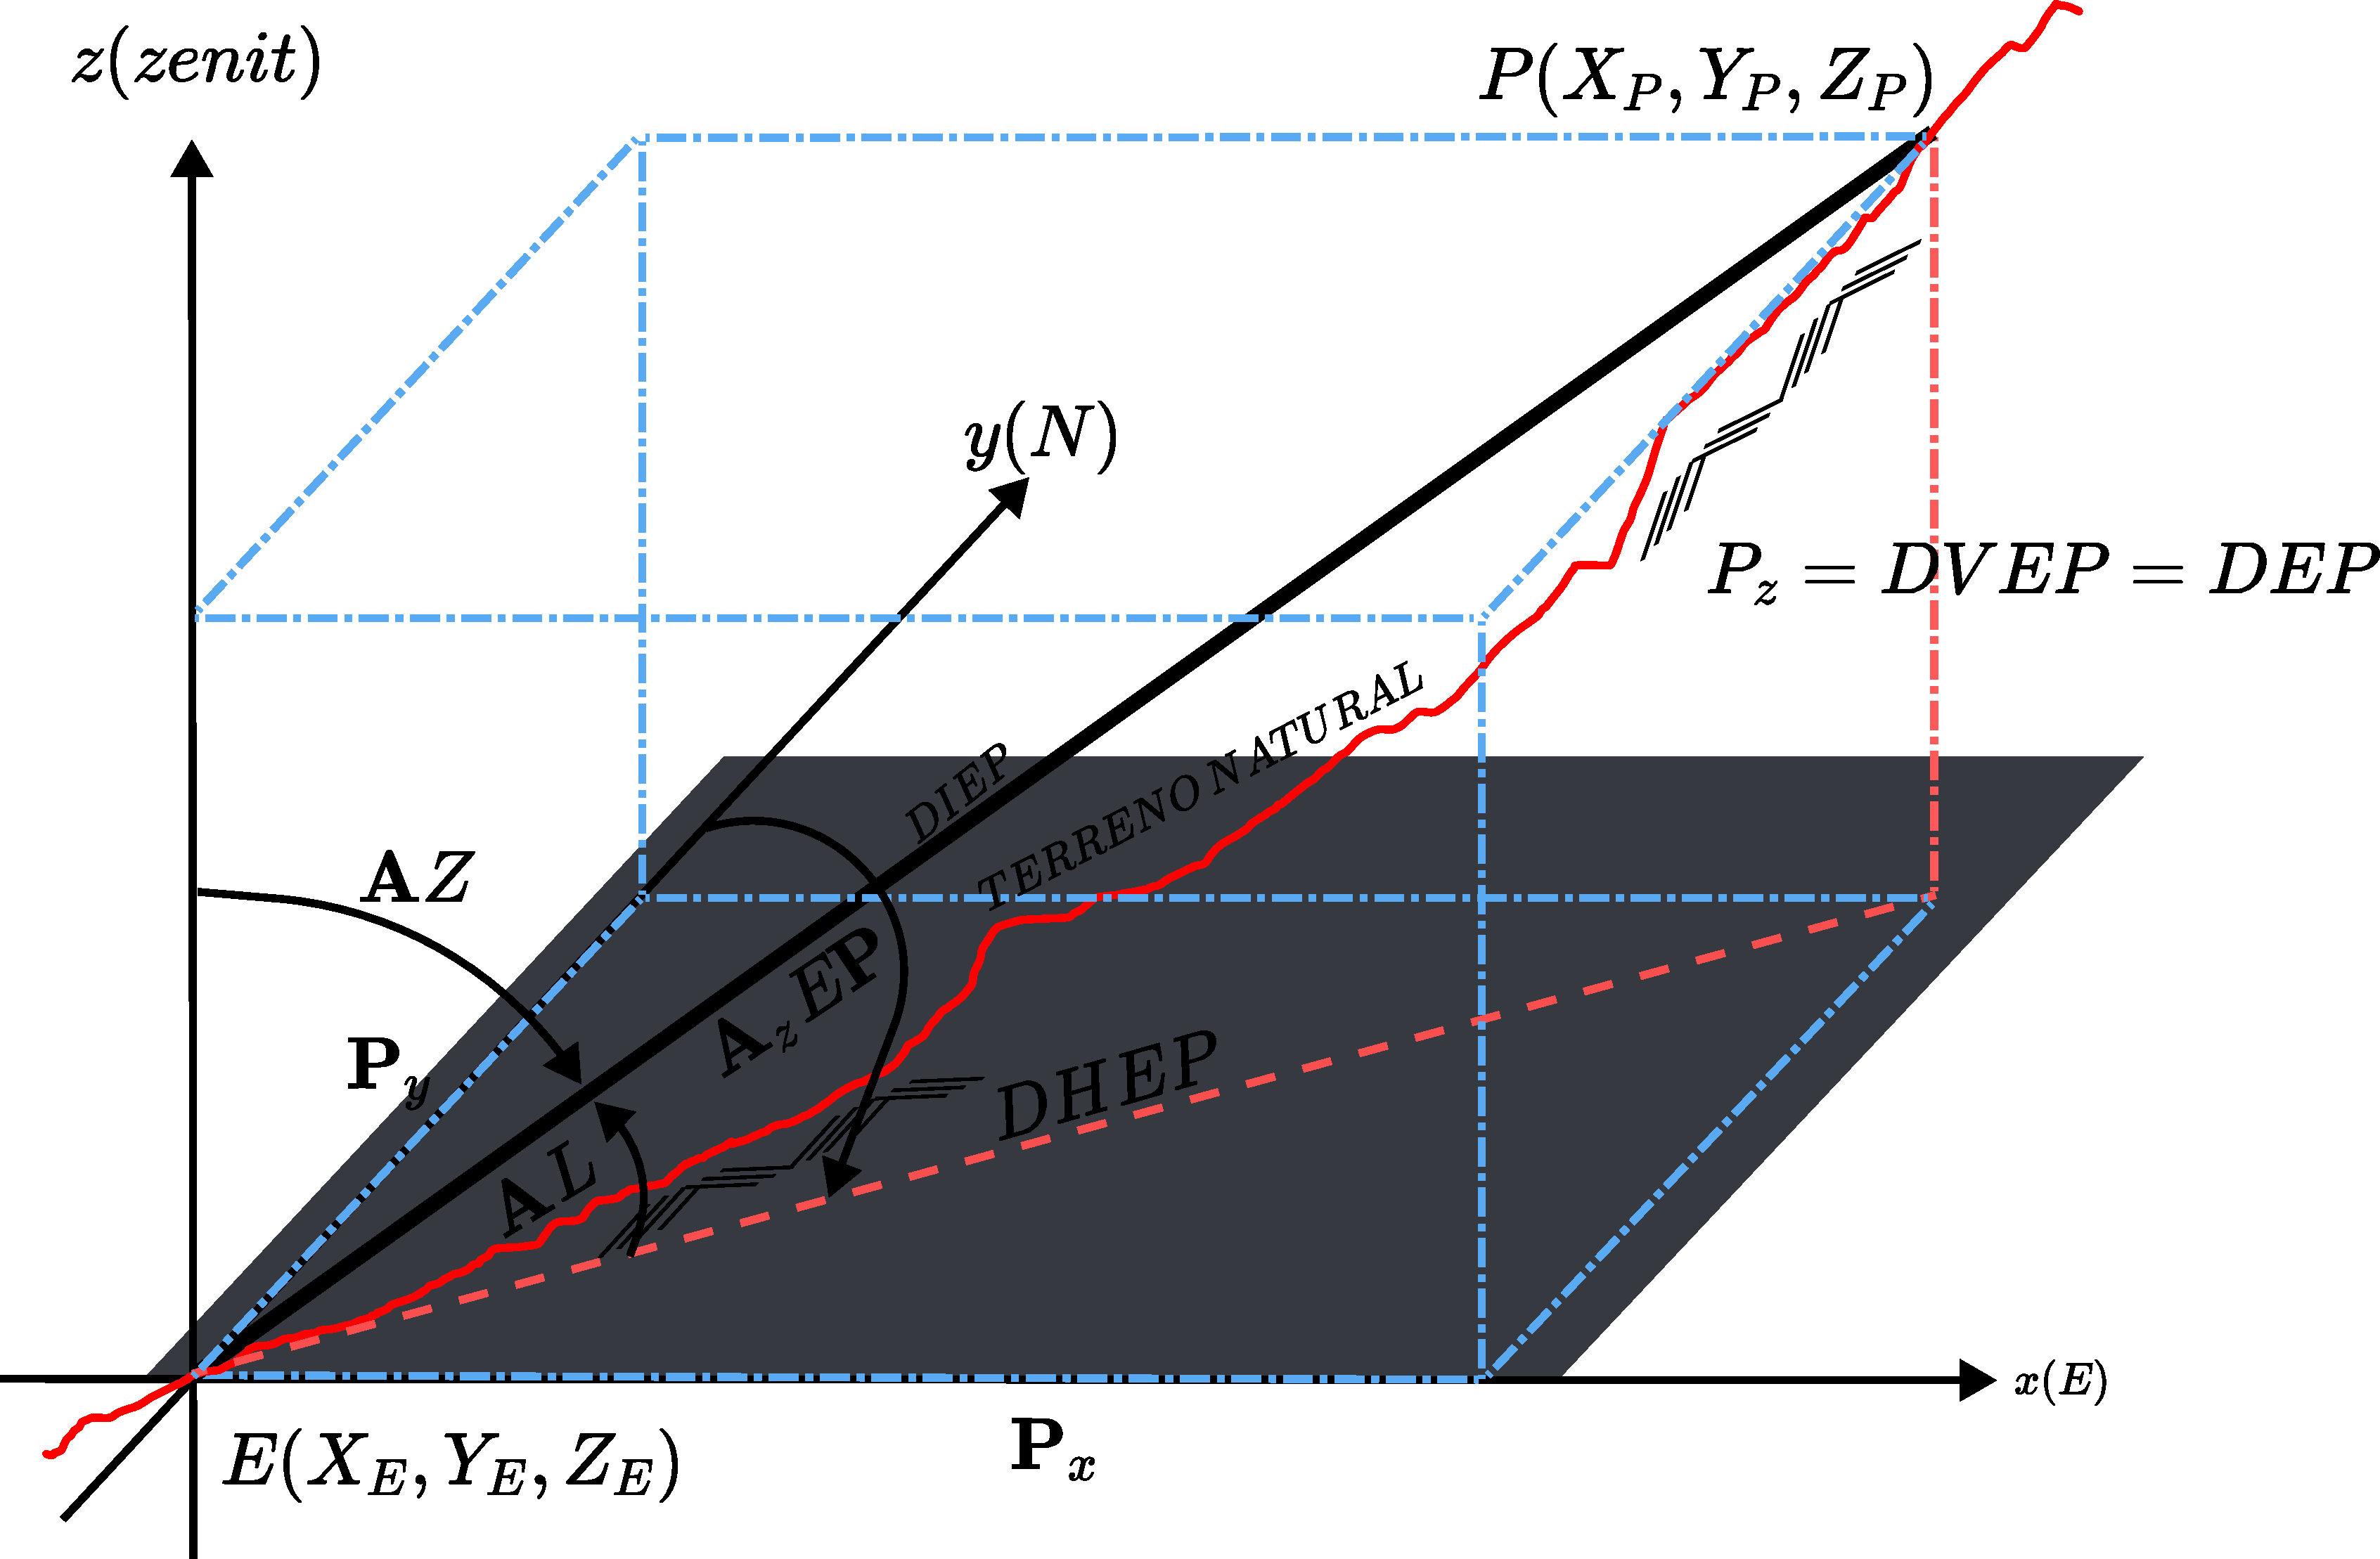
\includegraphics[width=0.5\textwidth]{ta6.pdf}}
  \caption{coordenadas}
  \label{ta6}
\end{figure}

\begin{align}
    &DH_{EP}=DI_{EP}\times \cos{AL_{EP}}\\ 
    &PZ_{EP}=DI_{EP}\times \sin{AL_{EP}}\\
    &DH_{EP}=DI_{EP}\times \sin{AZ_{EP}}\\
    &PZ_{EP}=DI_{EP}\times \cos{AZ_{EP}}
\end{align}

\begin{figure}[h!]
    \centerline{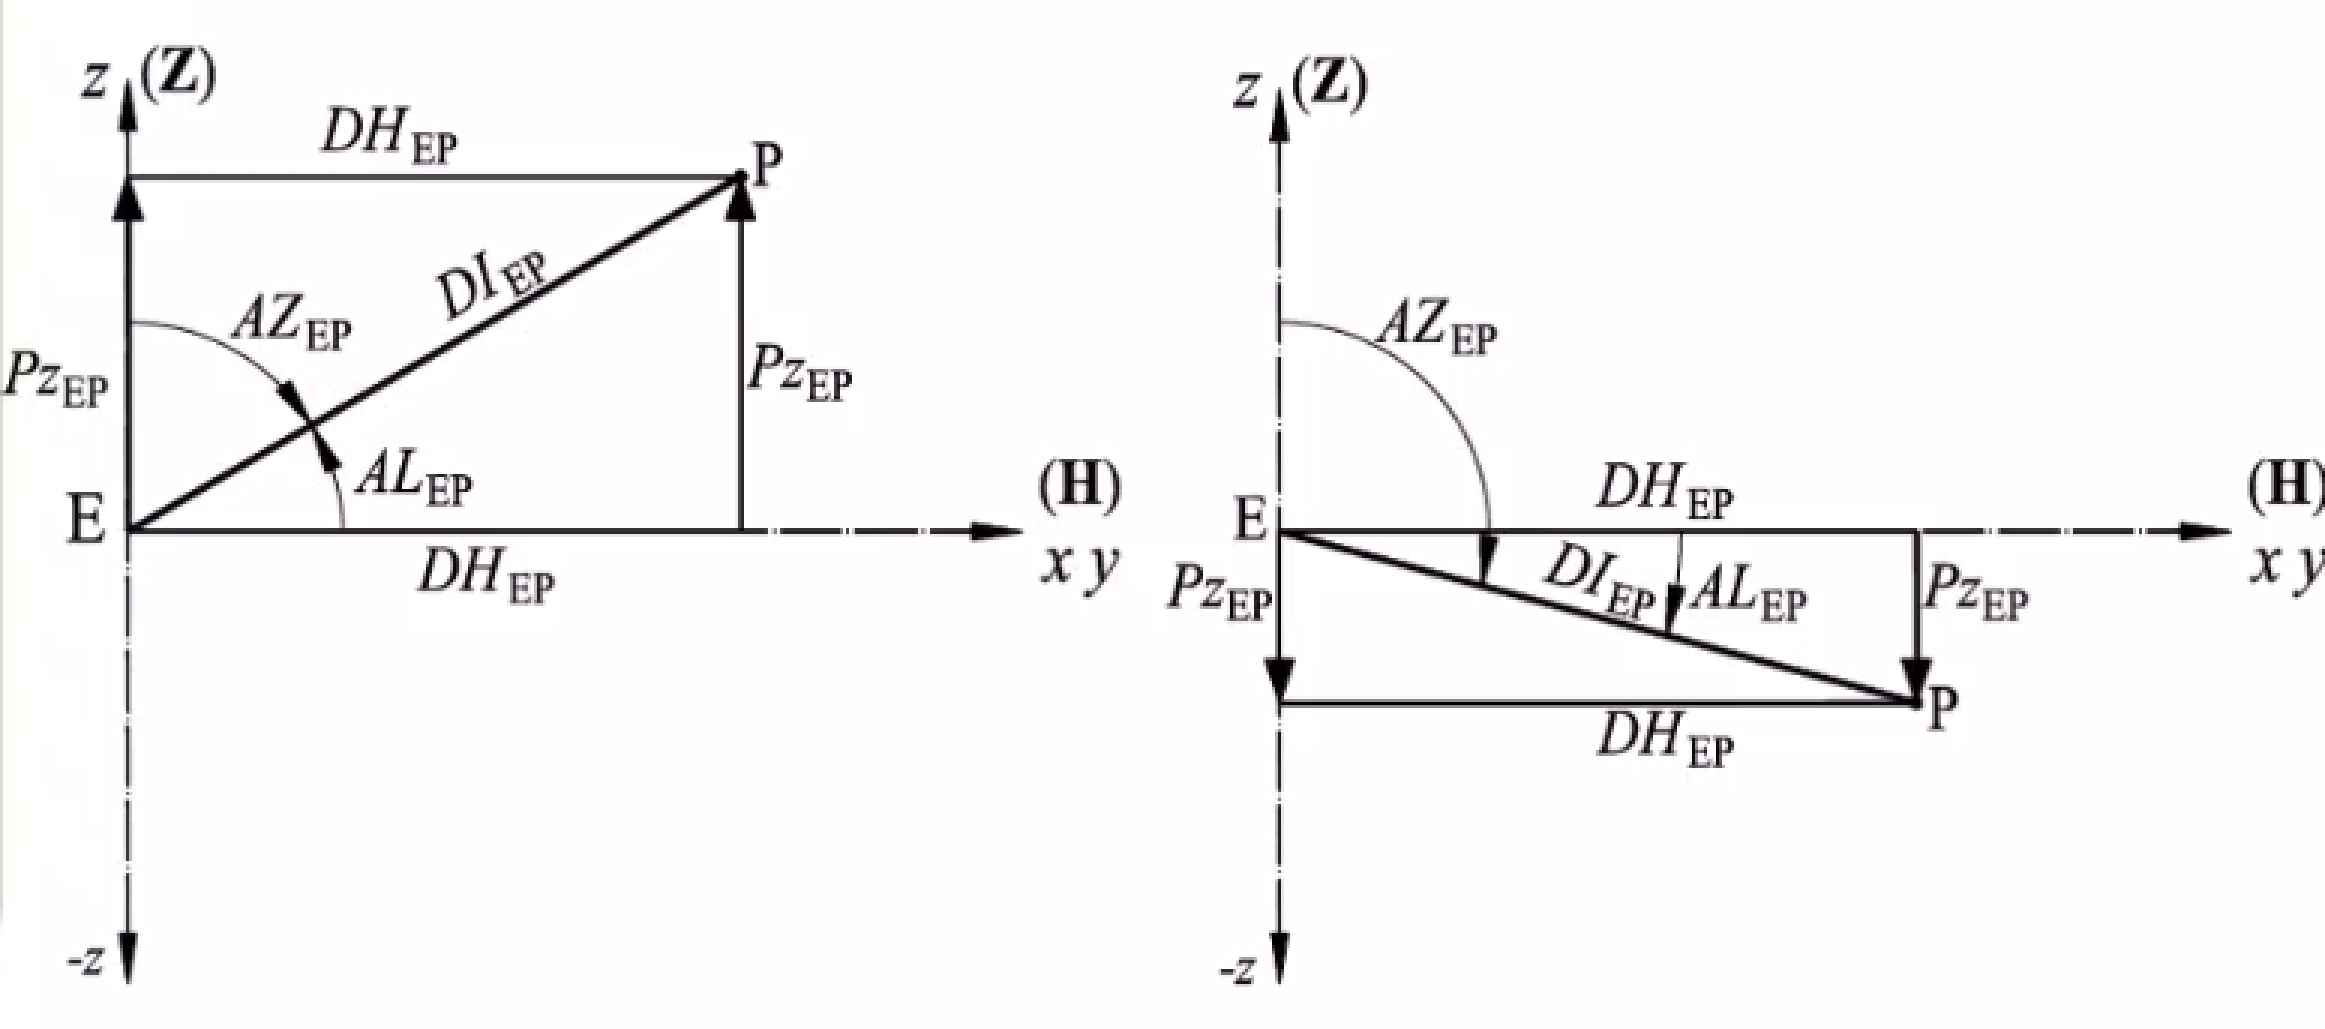
\includegraphics[width=0.5\textwidth]{ta7.png}}
    \caption{Cálculo de las proyecciones $DH$ y $P_Z$}
    \label{ta7}
\end{figure}

\begin{align}
    &P_{xEP}=DH_{EP}\times \sin{AZ_{EP}}\\
    &P_{yEP}=DH_{EP}\times \cos{AZ_{EP}}\\
\end{align}

\begin{table}[h!]
    \centering
    \begin{tabular}{@{}lll@{}}
        \toprule
        Cuadrante & $P_x$  & $P_y$ \\ \midrule
        NE        & +      & +     \\
        SE        & +      & -     \\
        SW        & -      & -     \\
        NW        & -      & +     \\ \bottomrule
    \end{tabular}
    \caption{Coordenada de puntos}
    \label{tabta4}
    \end{table}


\begin{figure}[h!]
    \centerline{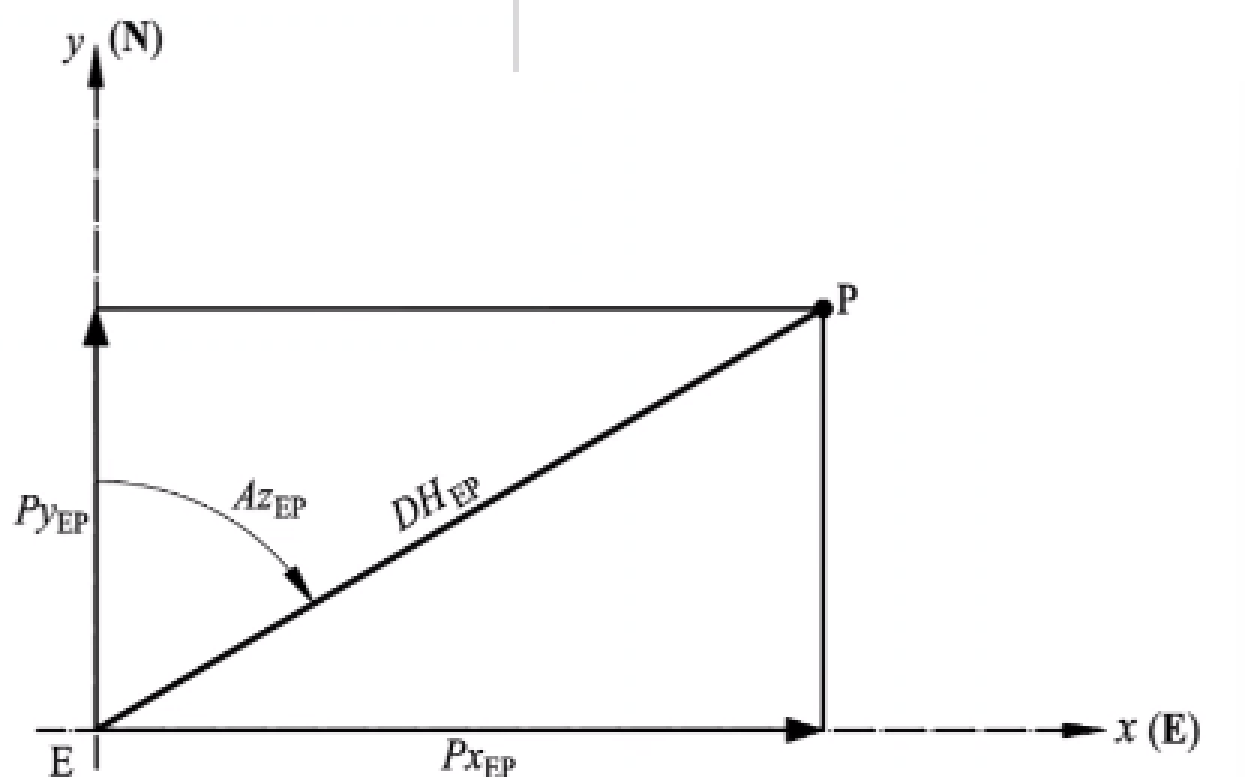
\includegraphics[width=0.5\textwidth]{ta8.png}}
    \caption{Cálculo de las proyecciones $DH$ y $P_Z$}
    \label{ta8}
\end{figure}

\begin{align}
    &DH_{EP}=100\times \left(LHS-LHI\right)\cos^2{(AL_v)}\\
    &DH_{EP}=100\times \left(LHS-LHI\right)\sin^2{(AZ_V)}\\
    &P_{zEP}=hi+\underbrace{50\times \left(LHS-LHI\right)}_{\text{Distancia vertical DV}}\sin{(2AL_v)}-LHM\\
    &P_{zEP}=hi+50\times \left(LHS-LHI\right)\sin{(2AZ_v)}-LHM
\end{align}

\begin{figure}[h!]
  \centerline{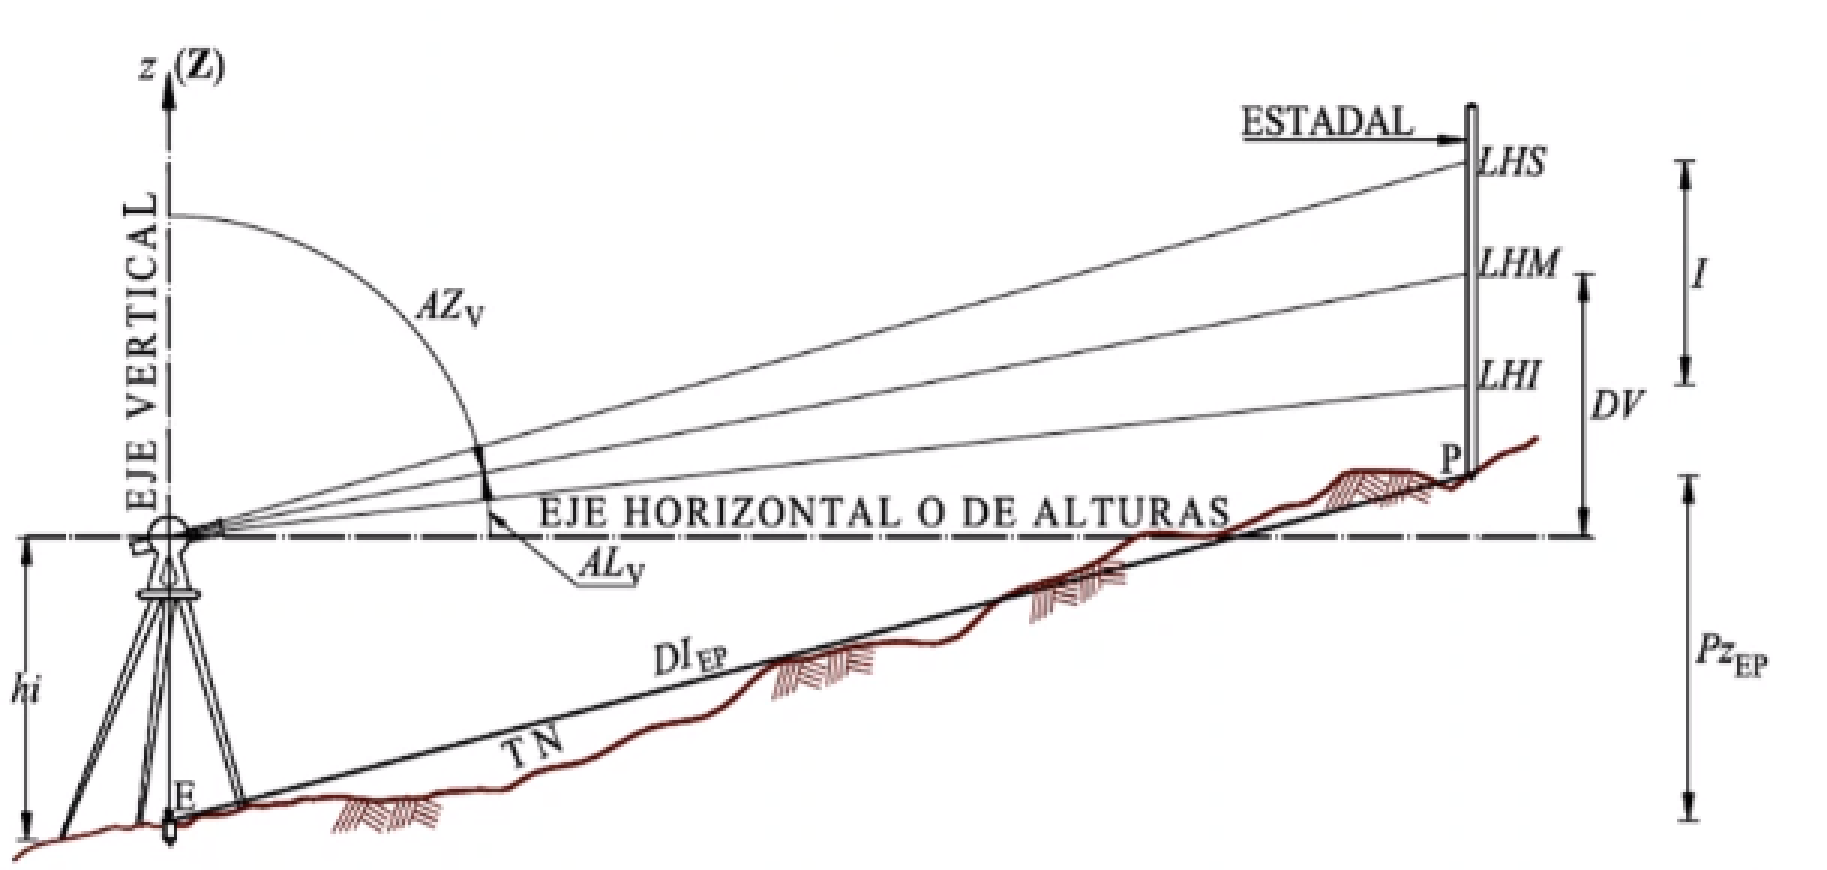
\includegraphics[width=0.5\textwidth]{ta9.png}}
  \caption{Proyecciones para levantamiento por Estadía}
  \label{ta9}
\end{figure}

\begin{notation}
    $h_i$=altura de la estadía
\end{notation}

\begin{example}
    Supóngase las siguientes coordenadas $X_E,Y_E,Z_E$ para el punto $E=\left[2,568.459;3758.289; 1874.983\right]$ y que se han medido para la línea $EP$ la distancia inclinada $DI_{EP}=284.123m$ el azimut $Az_{EP}=258^{\circ}15^{\prime}46^{\prime\prime}$ y la altura
    $AL_{EP}=-21^{\circ}56^{\prime}09^{\prime\prime}$ se trata de determinar las coordenadas del punto $P$. 
\end{example}

\textit{ Sol. }

A partir de la expresión y por considerar su uso más conveniente, se obtiene el ángulo cenital para la línea EP a partir del valor medido de AL

\begin{equation*}
    AZ_{EP}=90^{\circ}-AL_{EP}=90-\left(-21^{\circ}56^{\prime}09^{\prime\prime}\right)=111^{\circ}56^{\prime}09^{\prime\prime}
\end{equation*}

Aplicando este valor y el de la distancia inclinada proporcionando en las expresiones se obtienen los valores de la distancia horizontal $DH_{EP}$ y la proyección $Pz_{EP}$ de la línea $EP$
\begin{align*}
    &DH_{EP}=284.123\times \sin{(111^{\circ}56^{\prime}09^{\prime\prime})}=284.123\times \sin{111^{\circ}}=284.123\times \sin{22.5}=284.123\times \sin{0.5}=284.123\times \sin{0.087}=+263.533m\\
    &Pz_{E}=284.123\times \cos{(111^{\circ}56^{\prime}09^{\prime\prime})}=-106.139m
\end{align*}

Sustituyendo el valor obtenido de la distancia horizontal y el proporcionado del azimut de la línea EP, en las expresiones.
\begin{align*}
    &P-{xEP}=263.553\times \sin{\left(258^{\circ}15^{\prime}46^{\prime\prime}\right)}=-258.042m\\
    &Py_{EP}=263.553\times \cos{\left(258^{\circ}15^{\prime}46^{\prime\prime}\right)}=-53.619m\\
\end{align*}

Y sustituyendo los valores de las tres proyecciones, se obtienen las coordenadas $X_P,Y_P,Z_P$ respectivamente.
\begin{align*}
    &X_P=2568.459-258.042=2310.417m\\
    &Y_P=3758.289-53.619=3704.670m\\
    &Z_P=1874.983-106.139=1768.843m
\end{align*}

\subsubsection{Elementos de líneas}
\begin{align*}
    &DI_{EP}=\sqrt{\left(X_P-X_E\right)^2+\left(Y_P-Y_E\right)^2+\left(Z_P-Z_E\right)^2}=\sqrt{P_x^2+P_y^2+P_z^2}\\
    &DDH_{EP}=\sqrt{\left(X_P-X_E\right)^2+\left(Y_P-Y_E\right)^2})\sqrt{Px_{EP}^2+Py_{EP}^2}\\
    &DV_{EP}=Pz_{EP}=\sqrt{\left(Z_p-Z_E\right)^2}\\
    &DI_{EP}=\sqrt{\left(DH_{EP}-DV_{EP}\right)^2}
\end{align*}

Sobre los ángulos verticales, tenemos las siguientes ecuaciones:

\begin{align}
    &AL_{EP}=\arcsin{\left(\frac{Pz_{EP}}{DI_{EP}}\right)}\\
    &AZ_{EP}=90^{\circ}-AL_{EP}
\end{align}

En los ángulos horizontales (Rumbo y/o Azimut)

\begin{align}
    &R_{EP}=\arcsin{\left(\frac{\left\lvert Px_{EP}\right\rvert }{DH_{EP}}\right)}\\
    &R_{EP}=\arcsin{\left(\frac{\left\lvert Py_{EP}\right\rvert }{DH_{EP}}\right)}\\
    &A_{EP}=9\arctan{\left(\frac{\left\lvert Px_{EP}\right\rvert}{Py_{EP}}\right)}
\end{align}

Si $X_P>X_E$ y $Y_P>Y_E\implies$ Primer cuadrante \textbf{NE} $AZ=R$

Si $X_P>X_E$ y $Y_P<Y_E\implies$ Segundo cuadrante \textbf{SE} $AZ=180^{\circ}-R$

Si $X_P<X_E$ y $Y_P<Y_E\implies$ Tercer cuadrante \textbf{SW} $AZ=180^{\circ}+R$

Si $X_P<X_E$ y $Y_P>Y_E\implies$ Cuarto cuadrante \textbf{NW} $AZ=360^{\circ}-R$

\begin{figure}[h!]
    \centerline{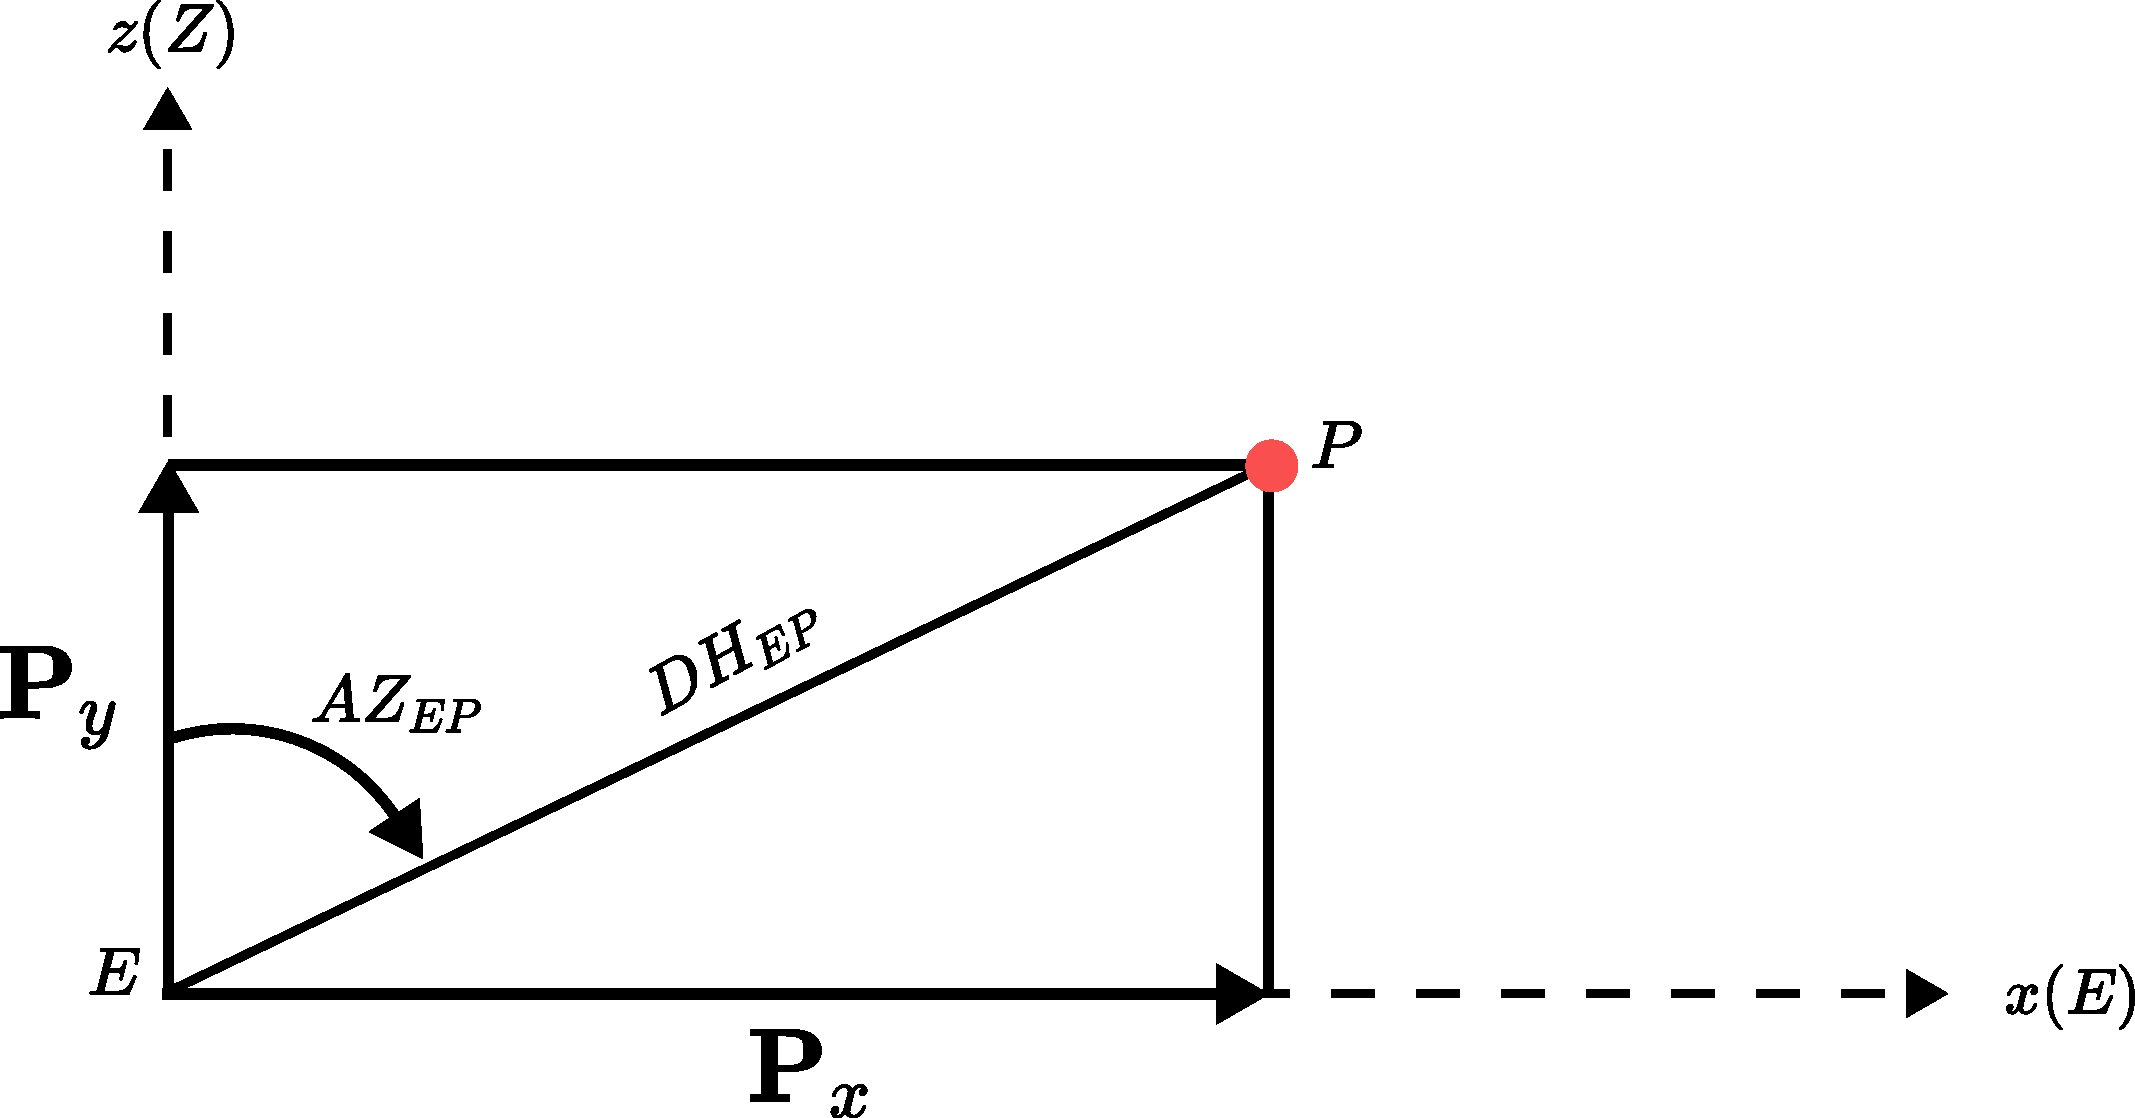
\includegraphics[width=0.5\textwidth]{ta10.pdf}}
    \caption{Ángulos horizontales}
    \label{ta10}
  \end{figure}

\begin{example}
    Se calculan los elementos lineales y angulares de la línea EP a partir de las coordenadas de los puntos E y P que la definen obtenidas en el ejercicio anterior y que se reproducen enseguida: $E\left[2568.459;3758.289;1874.983\right]$ y $P\left[2310.417;3704.670;1768.843\right]$
\end{example}

\textit{ Sol. }
\begin{align*}
    &Px_{EP}=X_P-X_E=2310.417-2568.459=-258.042m\\
    &Py_{EP}=Y_P-Y_E=3704.670-3758.289=-53.619m\\
    &Pz_{EP}=Z_P-Z_E=1768.843-1874.983=-106.140m\\
\end{align*}

Distancia 

Determinación de la altura y ángulo cenital de la línea EP: 
\begin{align*}
    &AL_{EP}=\arcsin{\left(\frac{-106.140}{284.124}\right)}=-21^{\circ}56^{\prime}9.29^{\prime\prime}\\
    &AZ_{EP}=90^{\circ}-\left(-21^{\circ}56^{\prime}9.29^{\prime\prime} \right)=111^{\circ}56^{\prime}9.29^{\prime\prime}
\end{align*}

\subsection{Sistemas coordenados esféricos y sistemas de proyección}

Hay dos posibilidades para su determinación. 

\begin{enumerate}
    \item Observaciones astronómicas
    \item Sistemas de posicionamiento Global
\end{enumerate}
\newpage
\begin{definition}[Latitud $\phi$]
    La latitud de un punto sobre la superficie terrestre, es el ángulo se mide en el centro de la tierra y que forma la vertical de ese punto con el plano del ecuador, con las siguientes características: se mide sobre el plano normal al ecuador que pasa por el punto a partir del ecuador, su valor varía de $0^{\circ}$ a $90^{\circ}$ hacia el Norte o hacia el Sur.
\end{definition}

\begin{definition}[Longitud]
    De un punto sobre la superficie terrestre, es el ángulo formado entre el meridiano que pasa por dicho punto y el meridiano de Greenwich tomado como origen, con las siguientes características: se mide en el plano del ecuador, a partir del meridiano de Greenwich, de $0^{\circ}$ a $360^{\circ}$ (0 a 24 horas) y hacia el Oeste, es decir en el sentido de las manecillas del reloj.
\end{definition}

La altitud, se define como la altura o distancia vertical en $m$ del punto desde el nivel medio del mar, medida sobre la vertical del lugar de observación en el sentido del Zenit y se denota por la letra mayúscula $Z$ y que coincide con la dirección del eje coordenado cartesiano z.

Se le llama esfera celeste a una esfera imaginaria de radio infinito con centro en el centro de la tierra.

Ambos son sentidos de giro definidos a partir del polo celeste, Oeste está en sentido horario y el Este en sentido antihorario

\begin{definition}[Declinación]
    La declinación $\delta$ de una estrella o de cualquier punto sobre la esfera celeste, es el ángulo formado entre el plano del ecuador celeste y la visual a dicha estrella; se mide en el plano del círculo horario que pasa por dicha estrella a partir del ecuador celeste de 0 a $90^{\circ}$ 
    hacia el norte positivo y al sur negativo
\end{definition}
\begin{definition}[Ascensión recta]
    denotado por $\alpha$, es el ángulo formado entre el círculo horario del punto vernal y el círculo horario que pasa por dicha estrella; se mide en el plano del ecuador celeste a partir del círculo horario del punto vernal, de 0 a $360^{\circ}$ hacia el Este\footnote{Distancia polar $p$ o codeclinación es el complemento de la declinación}
\end{definition}
\begin{equation}
    p=90^{\circ}-\delta
\end{equation}

\begin{figure}[h!]
  \centerline{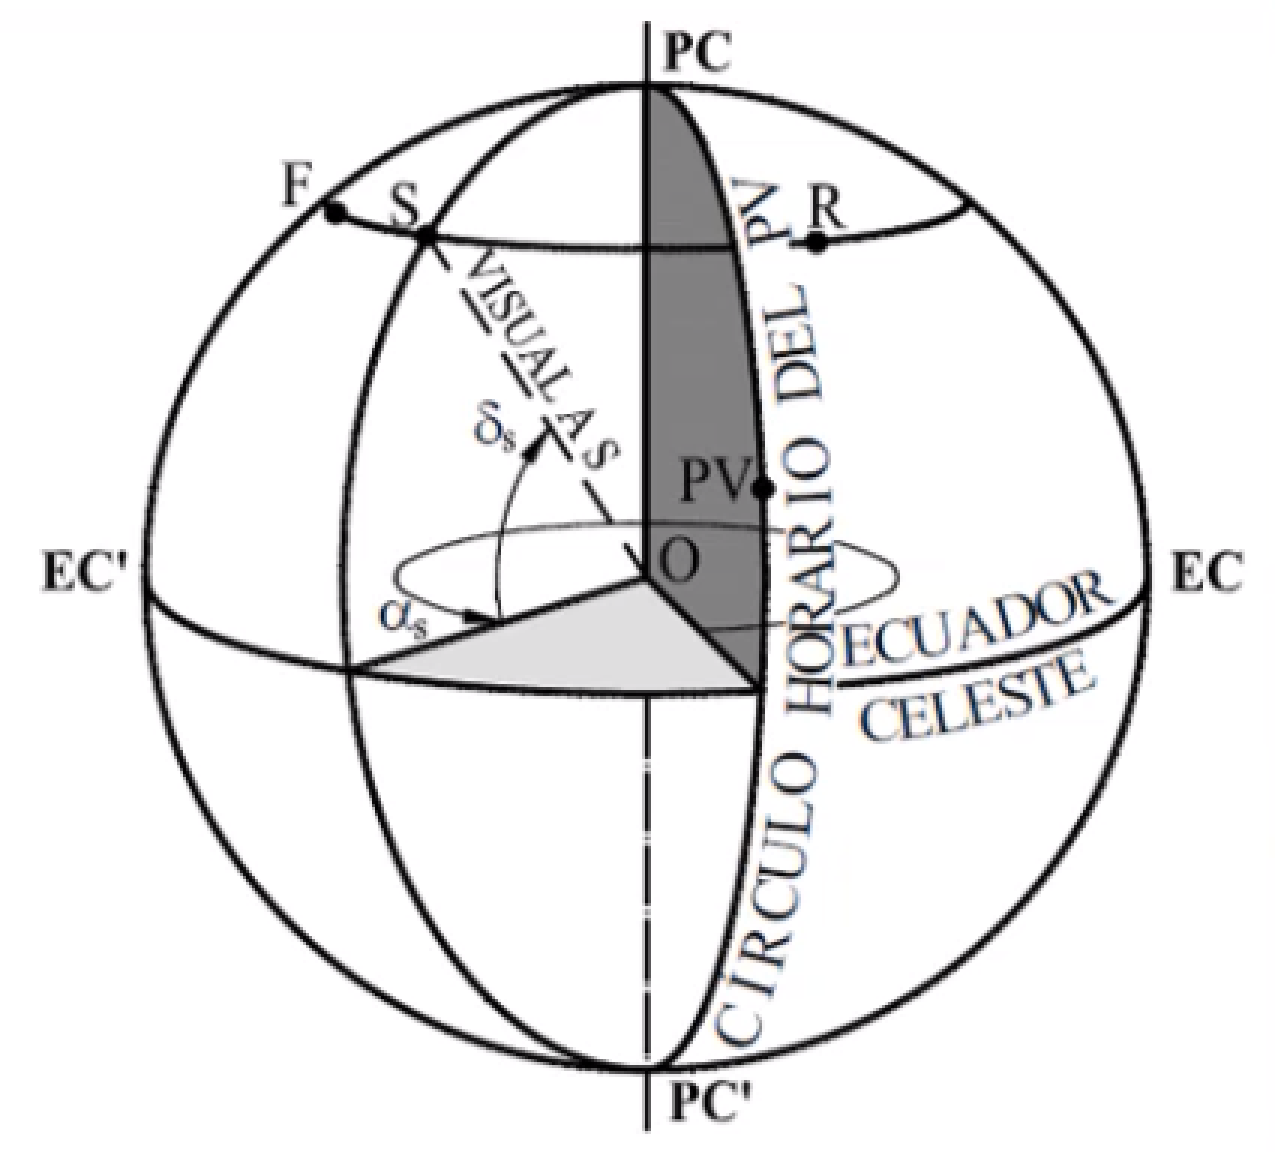
\includegraphics[width=0.5\textwidth]{ta11.png}}
  \caption{Coordenadas celestes ecuatoriales}
  \label{ta11}
\end{figure}

Distancia polar ($p$) o codeclinación es el complemento de la declinación

Un círculo máximo es una línea teórica que pasa a través del centro de la tierra y la divide en dos partes. El Ecuador y todos los meridianos son círculos máximos.

En la esfera celeste también hay círculos máximos
\begin{figure}[h!]
    \centerline{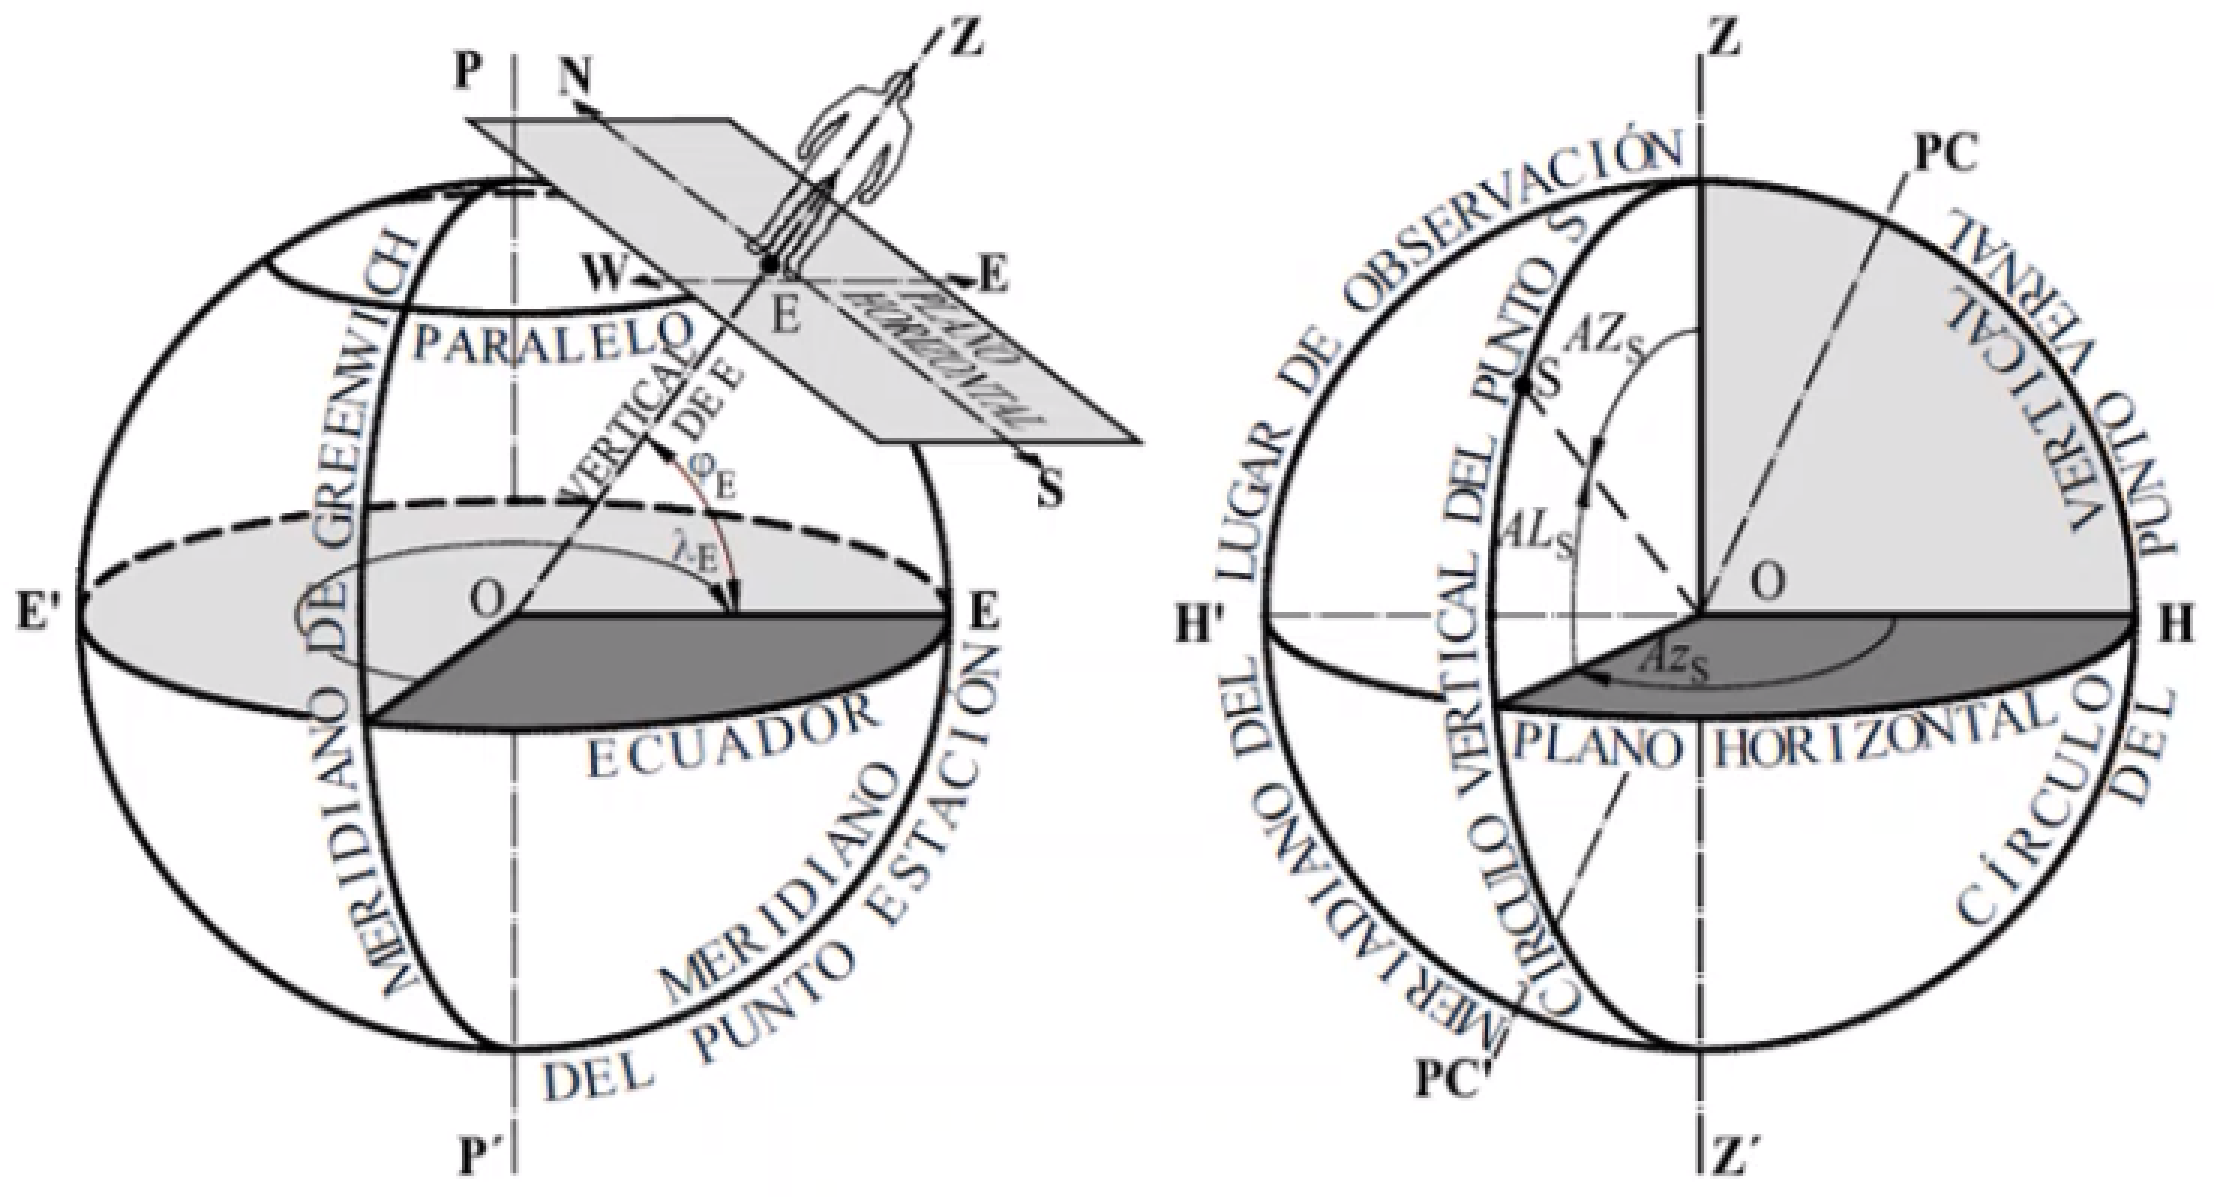
\includegraphics[width=0.5\textwidth]{ta12.png}}
    \caption{Sistemas coordenados esféricos. SCE celeste horizontal}
    \label{ta12}
  \end{figure}
  Los planos de referencia: 
\begin{itemize}
    \item \textbf{Plano principal:} EL plano horizontal del lugar de observación
    \item \textbf{Planos secundarios:} Círculos verticales (Círculos máximos que pasan por el cenit y el nadir)
    \item \textbf{Plano origen:} Meridiano del lugar de observación (meridiano y el círculo vertical simultáneamente)
\end{itemize}


\begin{definition}[La altura (AL) de una estrella]
    Es el ángulo formado entre el plano horizontal del lugar de observación y la visual de dicha estrella. Se mide en el plano del círculo vertical que pasa por la estrella a partir del plano horizontal del lugar de observación de $0^{\circ}$ a $90^{\circ}$
\end{definition}
El ángulo cenital $(AZ)$ se define como el complemento de la altura
\begin{definition}[Azimut de una estrella]
    Es el ángulo formado entre el meridiano del lugar de observación y el círculo vertical que pasa por la estrella, con las siguientes características: se mide en el plano horizontal del lugar de observación a partir del norte de $0^{\circ}$ a $360^{\circ}$ a 24 horas y hacia el oeste, es decir en el sentido de las manecillas del reloj
\end{definition}

\Schema{-1.4ex}{12ex}
{\schemabox{Sistemas\\Coordenados\\Esféricos}} { \Schema{-1ex}{4ex}
	{\schemabox{Terrestre}}
	{ \schema
		{\schemabox{Gravedad}}
		{\schemabox{Longitud $(\lambda)$\\
				Latitud $(\phi)$}}
	}
	\Schema{-1ex}{5ex}
	{\schemabox{Celestes}}
	{
		\vskip1ex\schema
		{\schemabox{Ecuatorial}}
		{\schemabox{Declinación $(\sigma)$\\ Ascensión recta $(\alpha)$}}
		\medskip
		\schema
		{\schemabox{Horizontal}}
		{\schemabox{Altura $(AL)$\\ Azimut $(AZ)$}}
	}
}

\subsubsection{Sistemas de proyección}
\begin{figure}[ht!]
	\begin{tikzpicture}[scale=1,every node/.style={minimum size=1cm}]
	%% some definitions
	
	\def\R{4} % sphere radius
	
	\def\angEl{25} % elevation angle
	\def\angAz{-100} % azimuth angle
	\def\angPhiOne{-50} % longitude of point P
	\def\angPhiTwo{-35} % longitude of point Q
	\def\angBeta{30} % latitude of point P and Q
	
	%% working planes
	
	\pgfmathsetmacro\H{\R*cos(\angEl)} % distance to north pole
	\LongitudePlane[xzplane]{\angEl}{\angAz}
	\LongitudePlane[pzplane]{\angEl}{\angPhiOne}
	\LongitudePlane[qzplane]{\angEl}{\angPhiTwo}
	\LatitudePlane[equator]{\angEl}{0}
	\fill[ball color=white!10] (0,0) circle (\R); % 3D lighting effect
	\coordinate (O) at (0,0);
	\coordinate[mark coordinate] (N) at (0,\H);
	\coordinate[mark coordinate] (S) at (0,-\H);
	\path[xzplane] (\R,0) coordinate (XE);
	
    %defining points outsided the area bounded by the sphere
	\path[qzplane] (\angBeta:\R+5.2376) coordinate (XEd);
	\path[pzplane] (\angBeta:\R) coordinate (P);%fino alla sfera
	\path[pzplane] (\angBeta:\R+5.2376) coordinate (Pd);%sfora di una quantità pari a 10 dopo la sfera
	\path[pzplane] (\angBeta:\R+5.2376) coordinate (Td);%sfora di una quantità pari a 10 dopo la sfera
	\path[pzplane] (\R,0) coordinate (PE);
    \path[pzplane] (\R+4,0) coordinate (PEd);
	\path[qzplane] (\angBeta:\R) coordinate (Q);
	\path[qzplane] (\angBeta:\R) coordinate (Qd);%sfora di una quantità pari a 10 dopo la sfera
	
	\path[qzplane] (\R,0) coordinate (QE);
    \path[qzplane] (\R+4,0) coordinate (QEd);%sfora di una quantità 10 dalla sfera sul piano equat.


    \DrawLongitudeCircle[\R]{\angPhiOne} % pzplane
    \DrawLongitudeCircle[\R]{\angPhiTwo} % qzplane
    \DrawLatitudeCircle[\R]{\angBeta}
    \DrawLatitudeCircle[\R]{0} % equator
	%labelling north and south
	\node[above=8pt] at (N) {$\mathbf{N}$};
	\node[below=8pt] at (S) {$\mathbf{S}$};
	
	\draw[-,dashed, thick] (N) -- (S);
	\draw[->] (O) -- (P);
	\draw[dashed] (XE) -- (O) -- (PE);
	\draw[dashed] (O) -- (QE);
	%connecting Points outside the sphere
	\draw[-,dashed,black,very thick] (O) -- (Pd);
	\draw[-,dashed,black,very thick] (O) -- (PEd);
    \draw[-,dashed,black,very thick] (O) -- (QEd);
    \draw[-,dashed,black,very thick] (O) -- (XEd);
    \draw[dashed] (XE) -- (O) -- (PE);
    %draw black thick flat grid
    \draw[-,ultra thick,black] (Pd) -- (PEd) node[below, left] {$P_1$};%verticale sinistro
    \draw[-,ultra thick,black] (PEd) -- (QEd)node[below, right] {$P_3$};%orizzontale inferiore
    \draw[-,ultra thick,black] (Pd)-- (XEd)node[above, right] {$P_2$};%orizzontale superiore	
    \draw[-,ultra thick,black] (XEd) -- (QEd);	
    		
	\draw[pzplane,->,thin] (0:0.5*\R) to[bend right=15]
	    node[midway,right] {$\lambda$} (\angBeta:0.5*\R);
	\path[pzplane] (0.5*\angBeta:\R) node[right] {$$};
	\path[qzplane] (0.5*\angBeta:\R) node[right] {$$};
	\draw[equator,->,thin] (\angAz:0.5*\R) to[bend right=30]
	    node[pos=0.4,above] {$\phi_1$} (\angPhiOne:0.5*\R);
	\draw[equator,->,thin] (\angAz:0.6*\R) to[bend right=35]
	    node[midway,below] {$\phi_2$} (\angPhiTwo:0.6*\R);
			\path[xzplane] (0:\R) node[below] {$$};
	\path[xzplane] (\angBeta:\R) node[below left] {$$};
    \foreach \t in {0,2,...,30} { \DrawLatitudeCirclered[\R]{\t} }
	\foreach \t in {130,133,...,145} { \DrawLongitudeCirclered[\R]{\t} }
	
	%drawing grids on the spere invoking DLongredd and DrawLongitudeCirclered
	
	\foreach \t in {130,145,...,145} { \DLongredd[\R+3]{\t} }
	\foreach \t in {130,133,...,145} { \DrawLongitudeCirclered[\R+3]{\t} }

	\foreach \t in {0,30,...,30} { \DLatred[\R+3]{\t} }
    \foreach \t in {0,2,...,30} { \DrawLatitudeCirclered[\R+3]{\t} }
	
    %labelling
    \draw[-latex,thick](4,-5.5)node[left]{Malla del Plano}
    	         to[out=0,in=270] (5.8,-2.3);
    \draw[thick](3.6,-6)node[left]{$[\mathsf{Rectilinea}]$};
    	
\end{tikzpicture}
	\caption[Representación de grillas computacionales esféricas y regulares utilizadas por SWAN]
     {Representación de sistemas de coordenadas esféricas (rojas) y cartesianas (negras). luego
     da un ejemplo de grillas no estructuradas. Ambos desestructurados.La conversión del primero al último implica un factor de deformación que es aceptable dentro de un límite espacial dado.}
\end{figure}

\begin{figure}[h!]
  \centerline{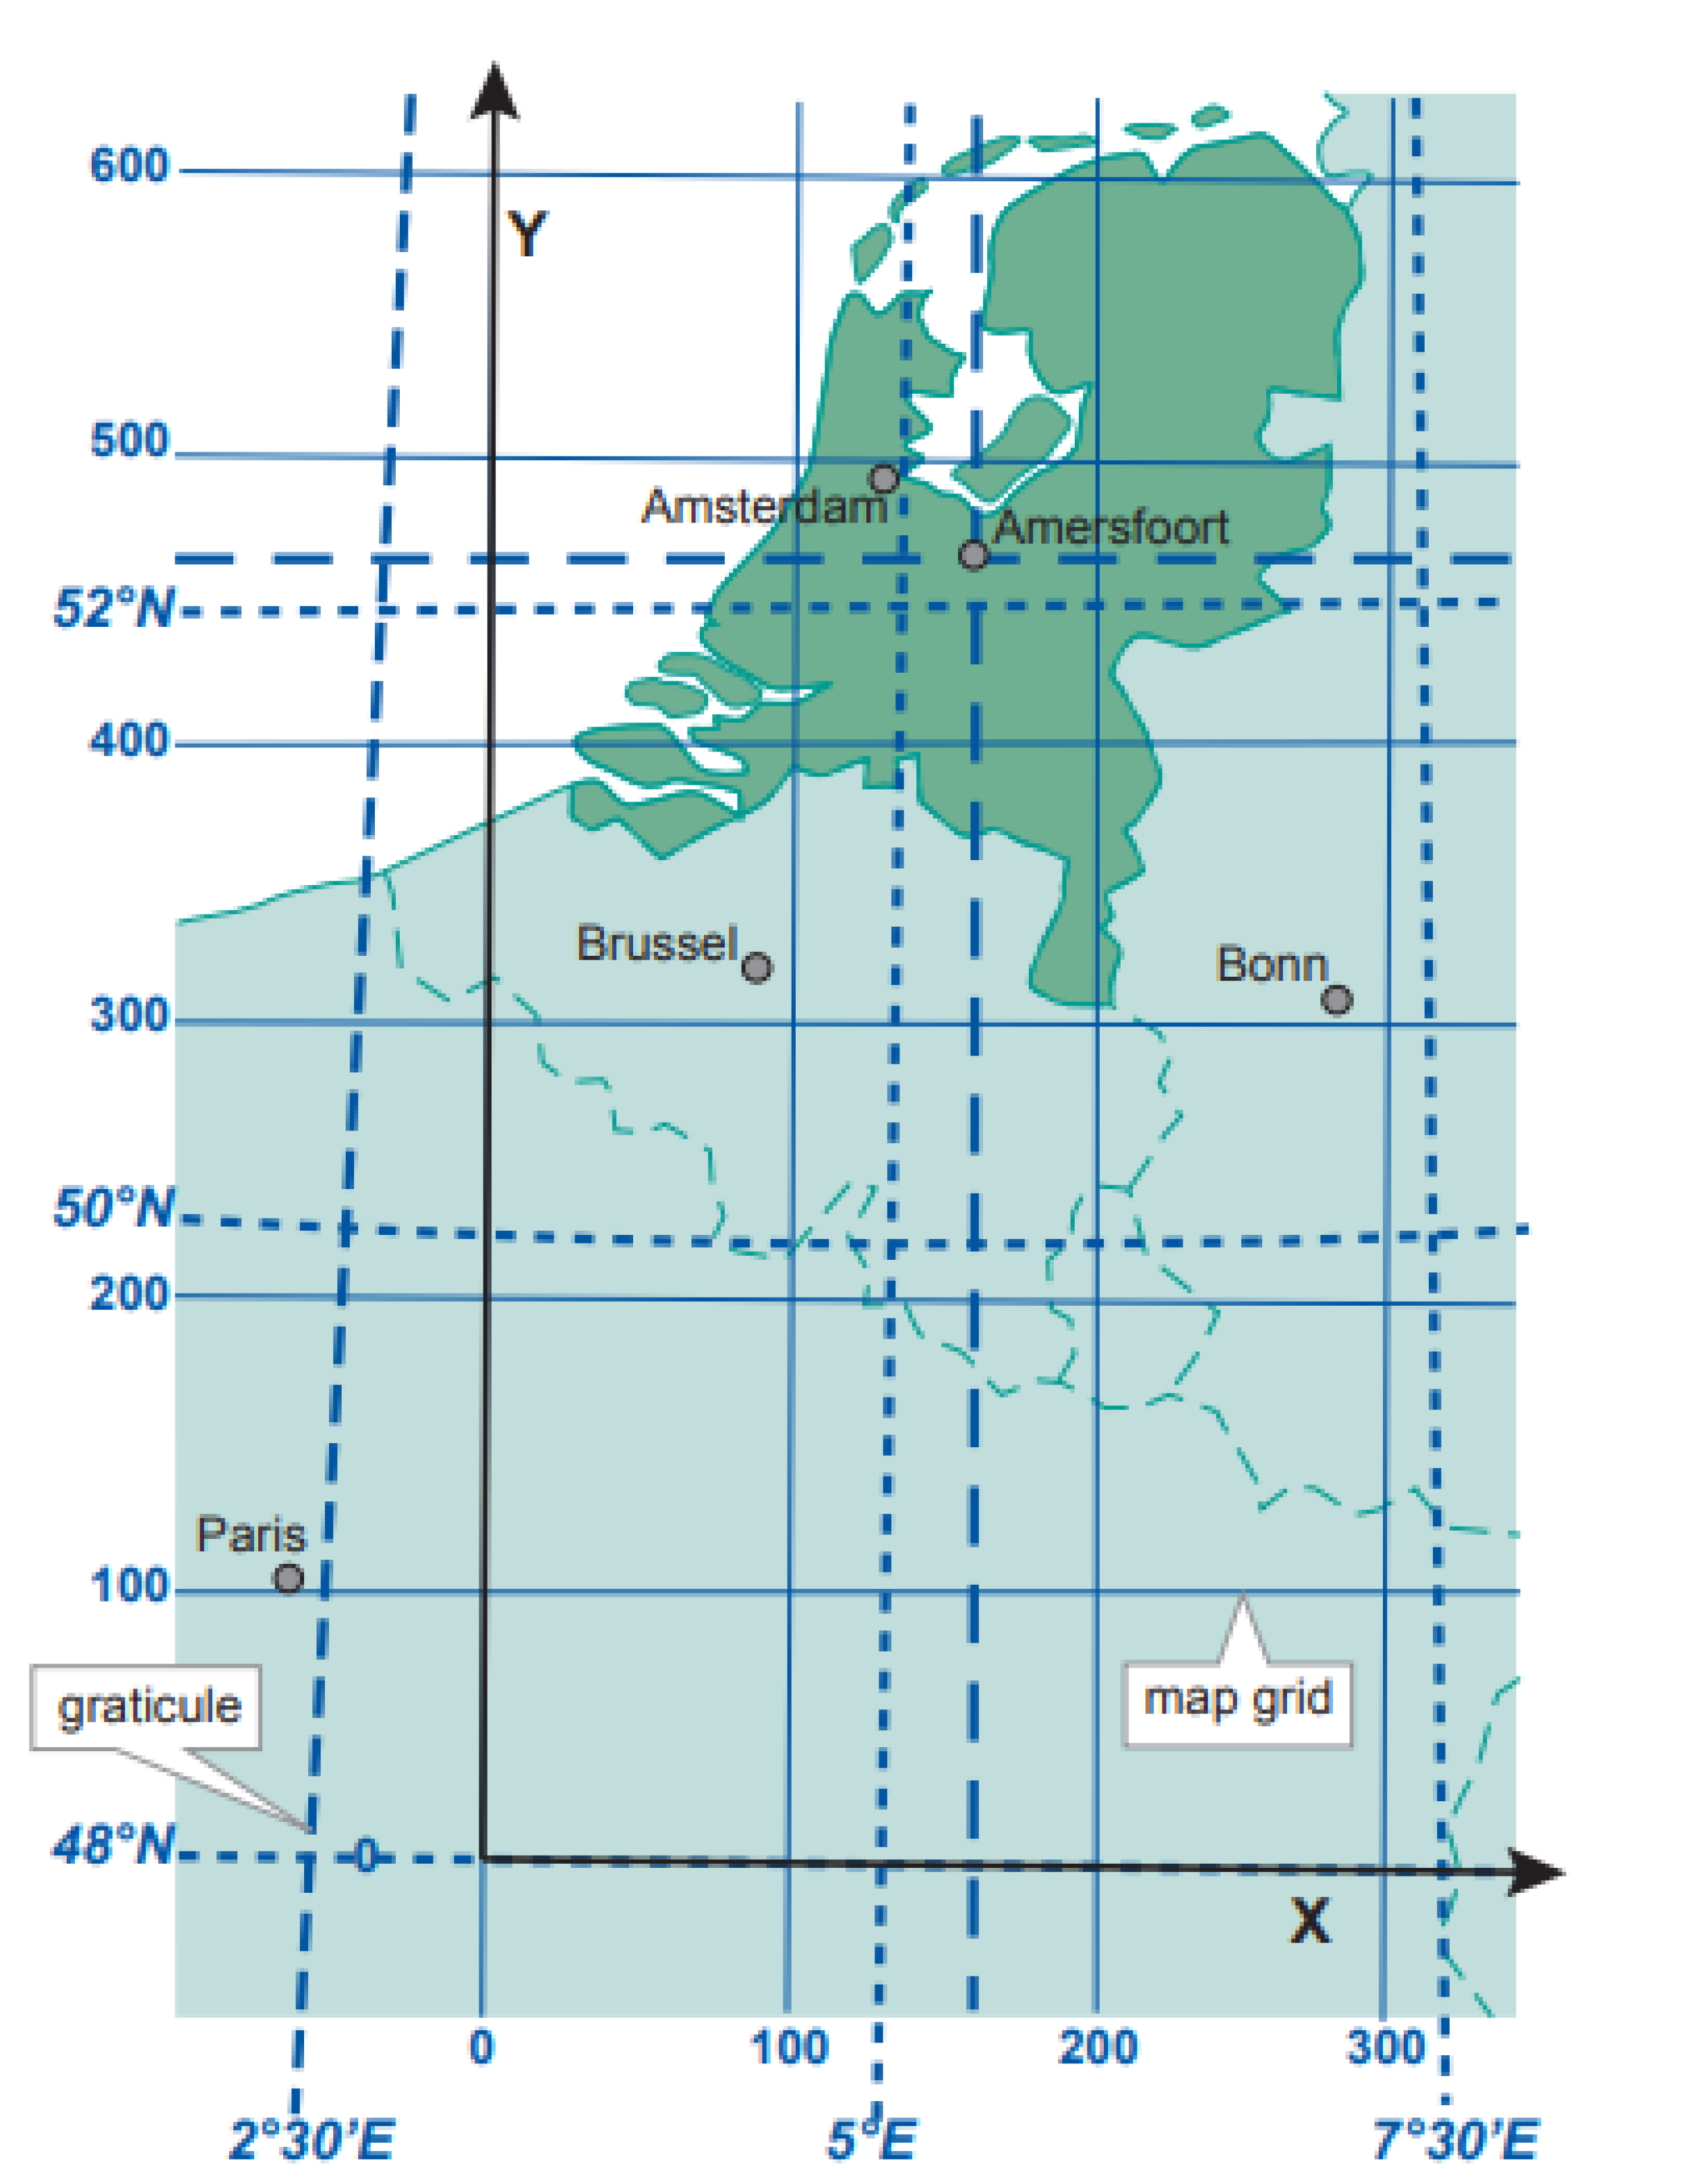
\includegraphics[width=0.5\textwidth]{ta14.png}}
  \caption{La proyección es un modelo matemático el cual transforma las coordenadas esféricas (latitud y longitud) en coordenadas planas (x,y) }
  \label{ta14}
\end{figure}

Existe un clasificación general de los sistemas de proyección más comunes (normal, transversal, diagonal)

La proyección transversa de Mercator puede describirse en general como en elipsoide proyectado dentro de un cilindro con tangencia establecida en el Ecuador y con el eje polar del elipsoide en coincidencia con el eje del cilindro.

A la Proyección de Mercator, en 1541 Por encargo de Carlos V, trazó diversos mapas, donde sobresalen dos globos (uno terráqueo y celeste) y el primer mapamundi para uso de navegantes, en 1569, en cuya elaboración utilizó un sistema de representación plana de la tierra llamado ``Proyección de Mercator'', en la superficie de proyección corresponde a la de un cilindro tangente al ecuador esférico.

El sistema Universal Transversa de Mercator (UTM), es el más utilizado mundialmente y consiste de una proyección cilíndrica transversal en la que la superficie terrestre comprendida entre los $84^{\circ}$ de latitud norte y los $80^{\circ}$ de latitud sur se divide en columnas, con un ancho de $6^{\circ}$ de longitud, llamadas zonas. Empezando a medir desde los $180^{\circ}$ le longitud oeste y desplazándose hacia el este, el mundo se divide en 60 zonas numeradas de 1 a 60. Cada columna está dividida a su vez, en cuadriláteros de una altura de $8^{\circ}$ de latitud, numerados con letras consecutivas desde la C hasta la X, empezando en los $8^{\circ}$ de latitud sur; de esta manera cada cuadrilátero se define por un número y una letra como en la figura 

%\begin{figure}[h!]
%  \centerline{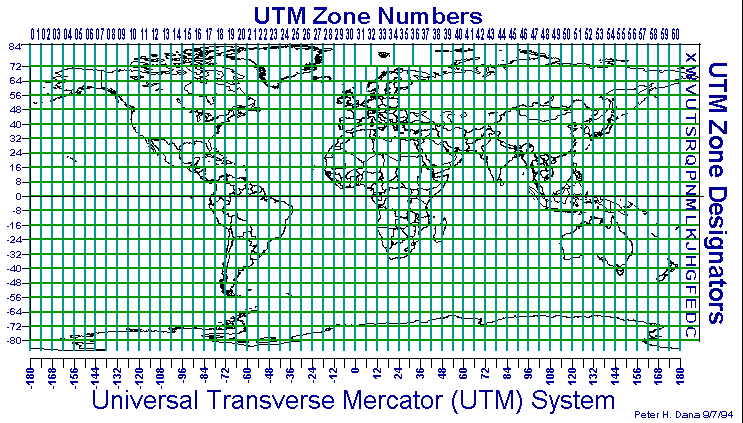
\includegraphics[width=0.5\textwidth]{ta15.png}}
%  \caption{UTM}
%  \label{ta15}
%\end{figure}

\subsubsection{Características de la zona UTM}

\begin{itemize}
    \item Los límites de una zona UTM coinciden con dos meridianos separados $6^{\prime}$ 
    \item El centro de la zona coincide con un meridiano, el meridiano central, que señala al norte
    \item El origen de la coordenada UTM es la intersección del meridiano central con el ecuador
\end{itemize}

Parámetros del elipsoide de Hayford. Se parte de los valores del semieje mayor $a=6.378388m$ t del semieje menor $b=6356911.946130m$  se obtiene la excentricidad $e$, la segunda excentricidad $e^{\prime}$ y el radio polar de cuadratura $c$

\begin{align}
    e=\frac{\sqrt{a^2-b^2}}{a}\\
    e^{\prime}=\frac{\sqrt{a^2-b^2}}{b}\\
    c=\frac{a^2}{b}
\end{align}

Obtención de los parámetros de Cotticia y Surace

\begin{align}
    &\lambda_0=int\left(\frac{\lambda}{6}\right)\times 6-3\\
    &\Delta \lambda=\lambda-\lambda_0\\
    &A=\cos{(\phi)}\times \sin{(\Delta \lambda)}\\
    &\xi=\frac{1}{2}\ln{\left(\frac{1+A}{1-A}\right)}\\
    &\eta=\arctan{\left(\frac{\tan{(\phi)}}{\cos{(\Delta\lambda)}}\right)}-\phi\\
    &v=\frac{0.9996c}{\left(1+e^2\times \cos^2{(\phi)}\right)^{\frac{1}{2}}}\\
    &\zeta=\frac{e^{\prime 2}}{2}\times\xi^2\cos{(\phi)}\\A_1
    &A=\sin{(2\phi)}\\
    &A_2=A_1\cdot\cos^2{(\phi)}
\end{align}

\begin{align}
    &J_2=\phi+\frac{A_1}{2}\\
    &D_4=\frac{3J_2+A_2}{4}\\
    &J_6=\frac{5J_4+A_2\cos^2{(\phi)}}{3}\\
    &\alpha=\frac{3}{4}e^{\prime 2}\\
    &\beta=\frac{5}{3}3\alpha^2\\
    &\gamma=\frac{35}{27}\alpha^{3}
\end{align}

Determinación de las coordenadas UTM Las coordenadas $X$ y $Y$ en el sistema de proyección Universal Transversa de Mercator se obtienen aplicando las expresiones
\begin{align}
    &X=\xi \left(1+\frac{\zeta}{3}\right)+500000\\
    &Y=\eta v(1+\zeta)+B\phi
\end{align}

\subsection{Puntos de Poligonales}

El procedimiento topográfico planimétrico de poligonal consiste en una serie de líneas de control y apoyo que ligan o conectan puntos de control y apoyo sucesivos, que se establecen en los sitios más convenientes desde el punto de vista del área que dominan para el posterior levantamiento de PCD

No importa la magnitud ni orientación de las LCA ni la magnitud de los ángulos, lo cual significa que este PTP no tiene ninguna condición geométrica que cumplir

Se debe cuidar que desde cada PCA se observa el anterior y el siguiente para la medición de ángulos y distancias y que desde cada pCA se domine la mayor área posible para levantar PCD

Las poligonales pueden ser abiertas o cerradas, en las cerradas el trazo regresa al pCA de partida formándose un polígono cerrado; en contraste las abiertas se trazan de modo que no se regresa al punto de partida, sino que por el contrario se alejan de él.

Las poligonales abiertas o cerradas constituyen el procedimiento topográfico de uso más frecuente, debido seguramente a que, por un lado son fáciles de trazar y a que su aplicabilidad es la más amplia por otro

Las poligonales cerradas, se aplican al levantamiento de terrenos agrícolas de lagunas decenas o incluso cientos de hectáreas, en el levantamiento de cuencas de captación y vasos de almacenamientos, entre otros;

Las poligonales abiertas, se usan comúnmente en el levantamiento de vías de comunicación, cauces y en general en áreas que se extienden en dirección determinada

En un estudio topográfico con poligonales, siempre es posible a menudo necesario usar una combinación de Poligonales abiertas y cerradas

La medición de líneas de control y apoyo de una poligonal abierta o cerrada, se hace del modo más simple y económico que dé la precisión requerida.

Invariablemente, se deben medir las distancias horizontales, con cinta se deben hacer las mediciones evitando errores de catenaria, de temperatura, por desnivel

\begin{figure}[h!]
  \centerline{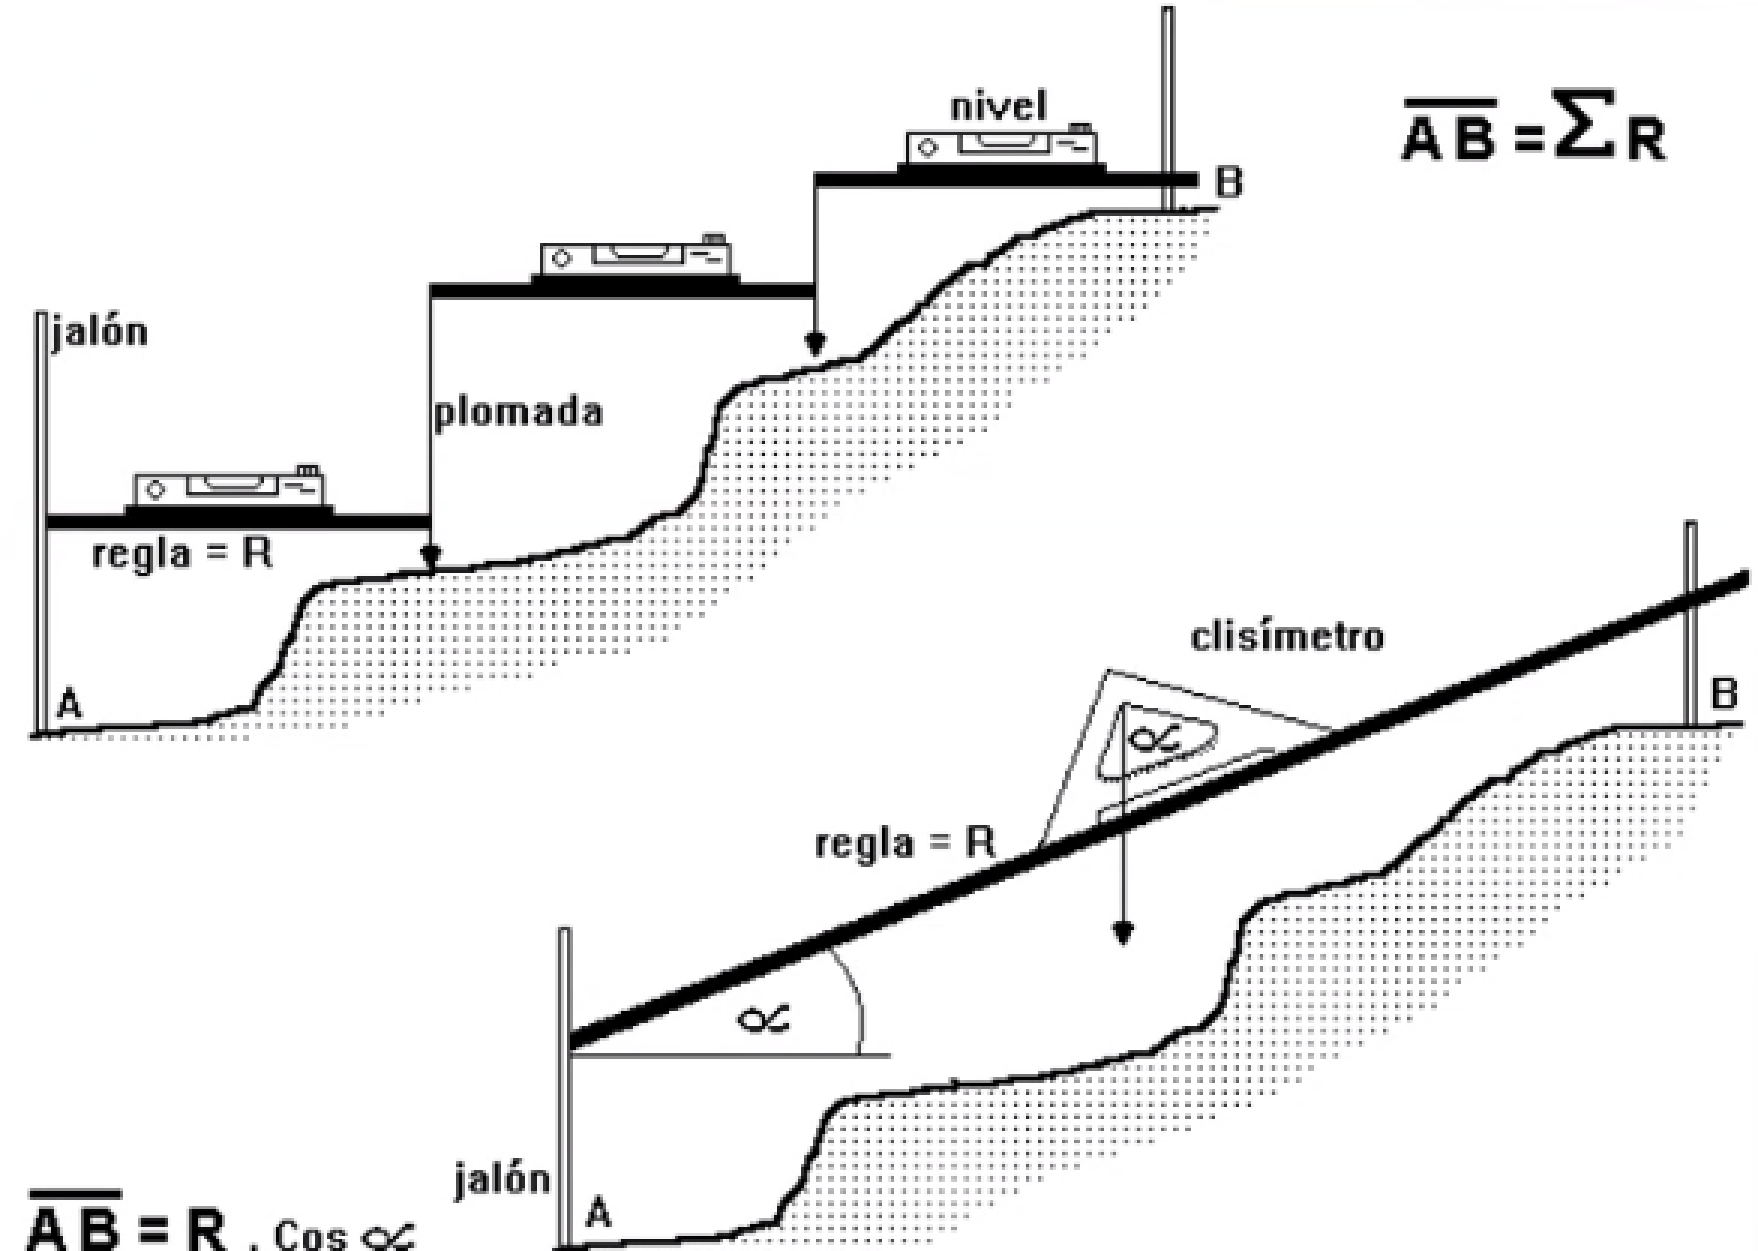
\includegraphics[width=0.5\textwidth]{ta16.png}}
  \caption{Trazo, mediciones lineales}
  \label{ta16}
\end{figure}

con tránsito o teodolito y estadal (ESTADIA) las DH se estiman con la fórmula de estadía.

\begin{align}
    DH_{EP}=100\times \left(LHS-LHI\right)\cos^2{AL_V}\\
    DH_{EP}=100\times \left(LHS-LHI\right)\sin^2{AZ_V}
\end{align}

\begin{figure}[h!]
  \centerline{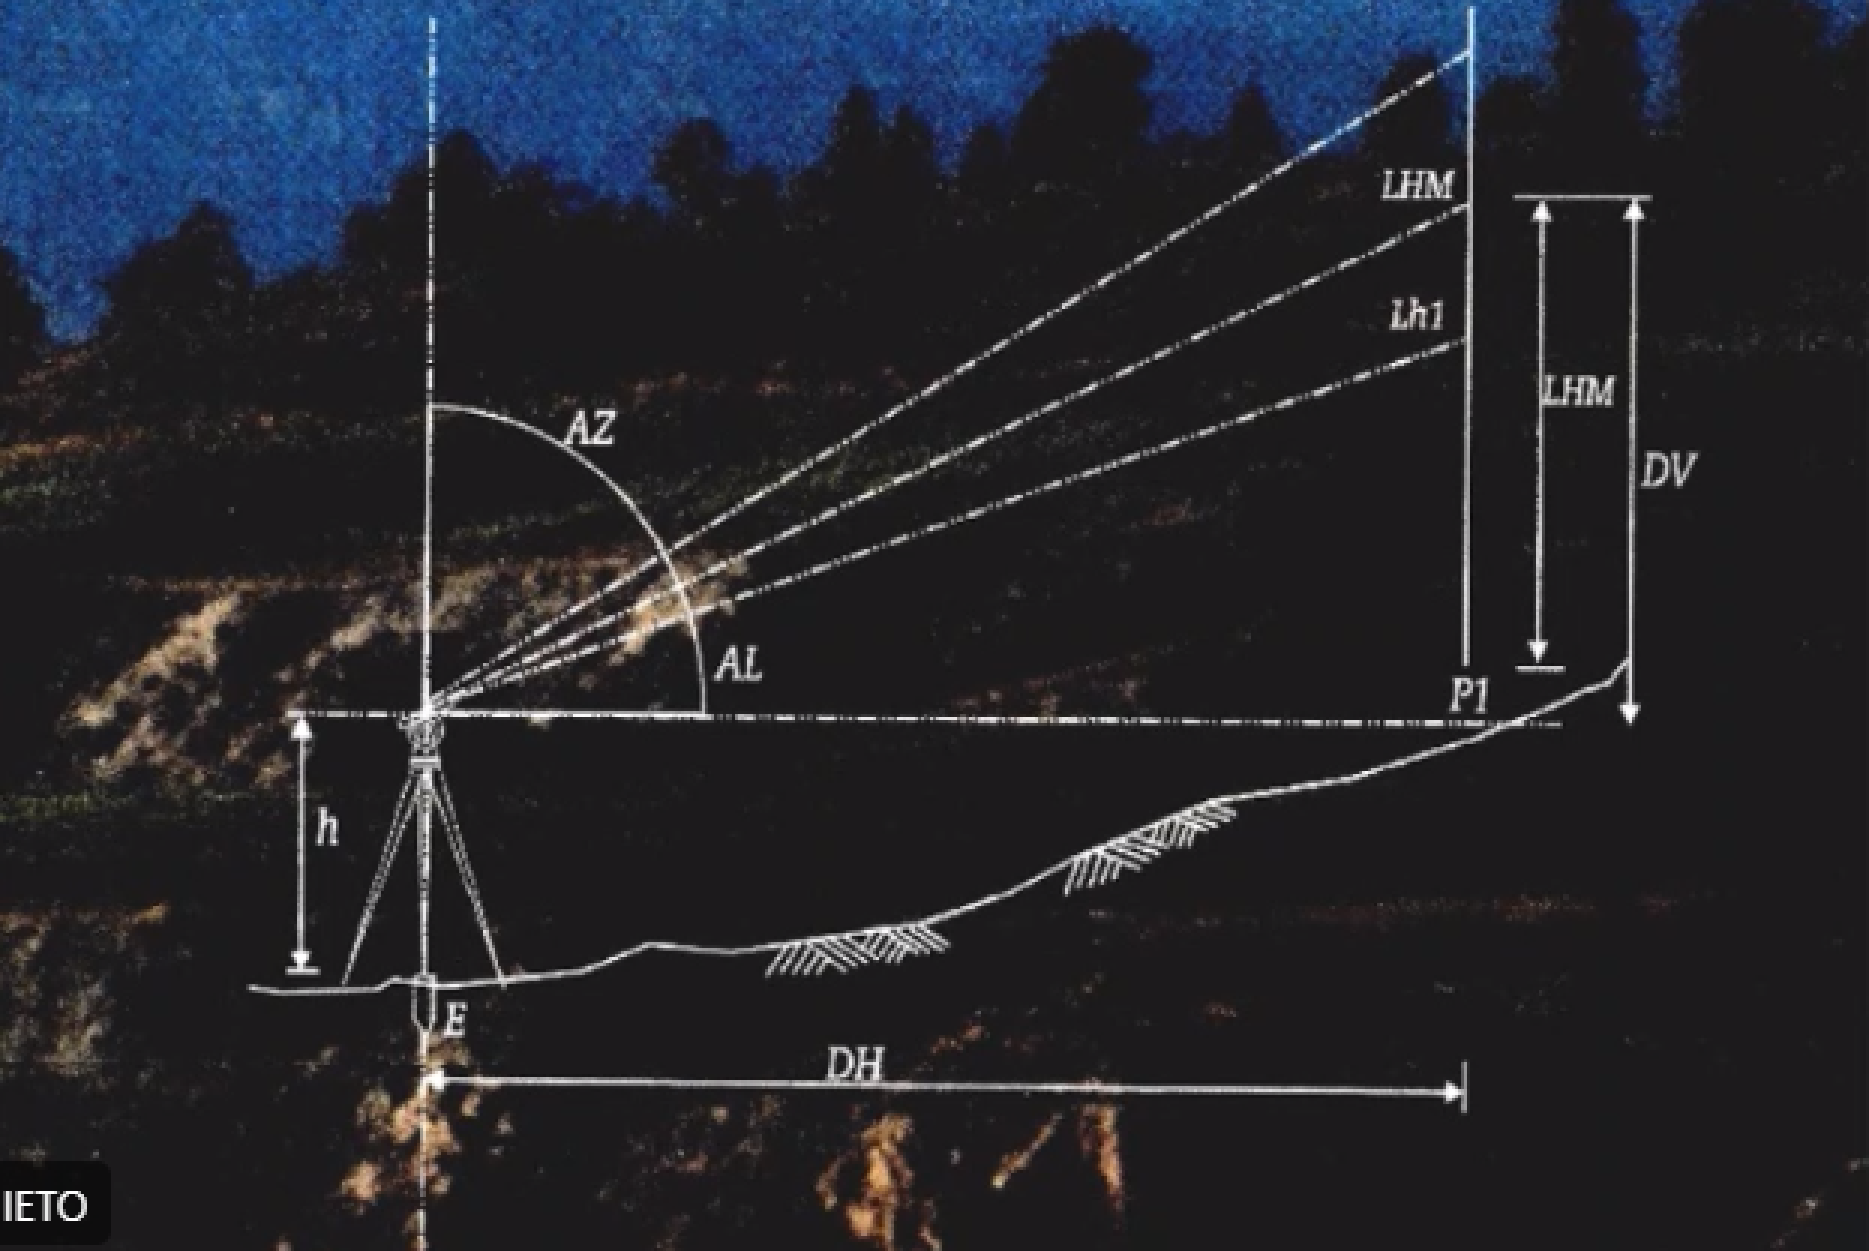
\includegraphics[width=0.5\textwidth]{ta17.png}}
  \caption{Medición en la práctica}
  \label{ta17}
\end{figure}

Con medidor electrónico de distancias (MED), la medición es más rápida, más precisa y de mayor longitud. también se puede con estación.

Las mediciones angulares en el establecimiento de una poligonal (y en general en cualquier procedimiento topográfico), se requieren para poder definir las direcciones de las líneas de control y apoyo

Mediciones angulares:

Se estaciona el instrumento (Tránsito, teodolito, estación total) en un PCA y se miden un ángulo según el método seleccionado: 

\begin{itemize}
    \item Ángulos internos (AI), figura \ref{ta18}
    \item Ángulos Externos (AE), figura \ref{ta18}
    \item Medición de azimuts (Az) o Rumbos (R), figura \ref{ta19}
    \item Medición  de ángulos de deflexión para poligonales abiertas, figura \ref{ta20}
    \item Medición de ángulos a la derecha (o al a izquierda) para ambos tipos de poligonal, figura \ref{ta21}
\end{itemize}



\begin{figure}[h!]
    \centering
    \begin{subfigure}[b]{0.45\linewidth}
    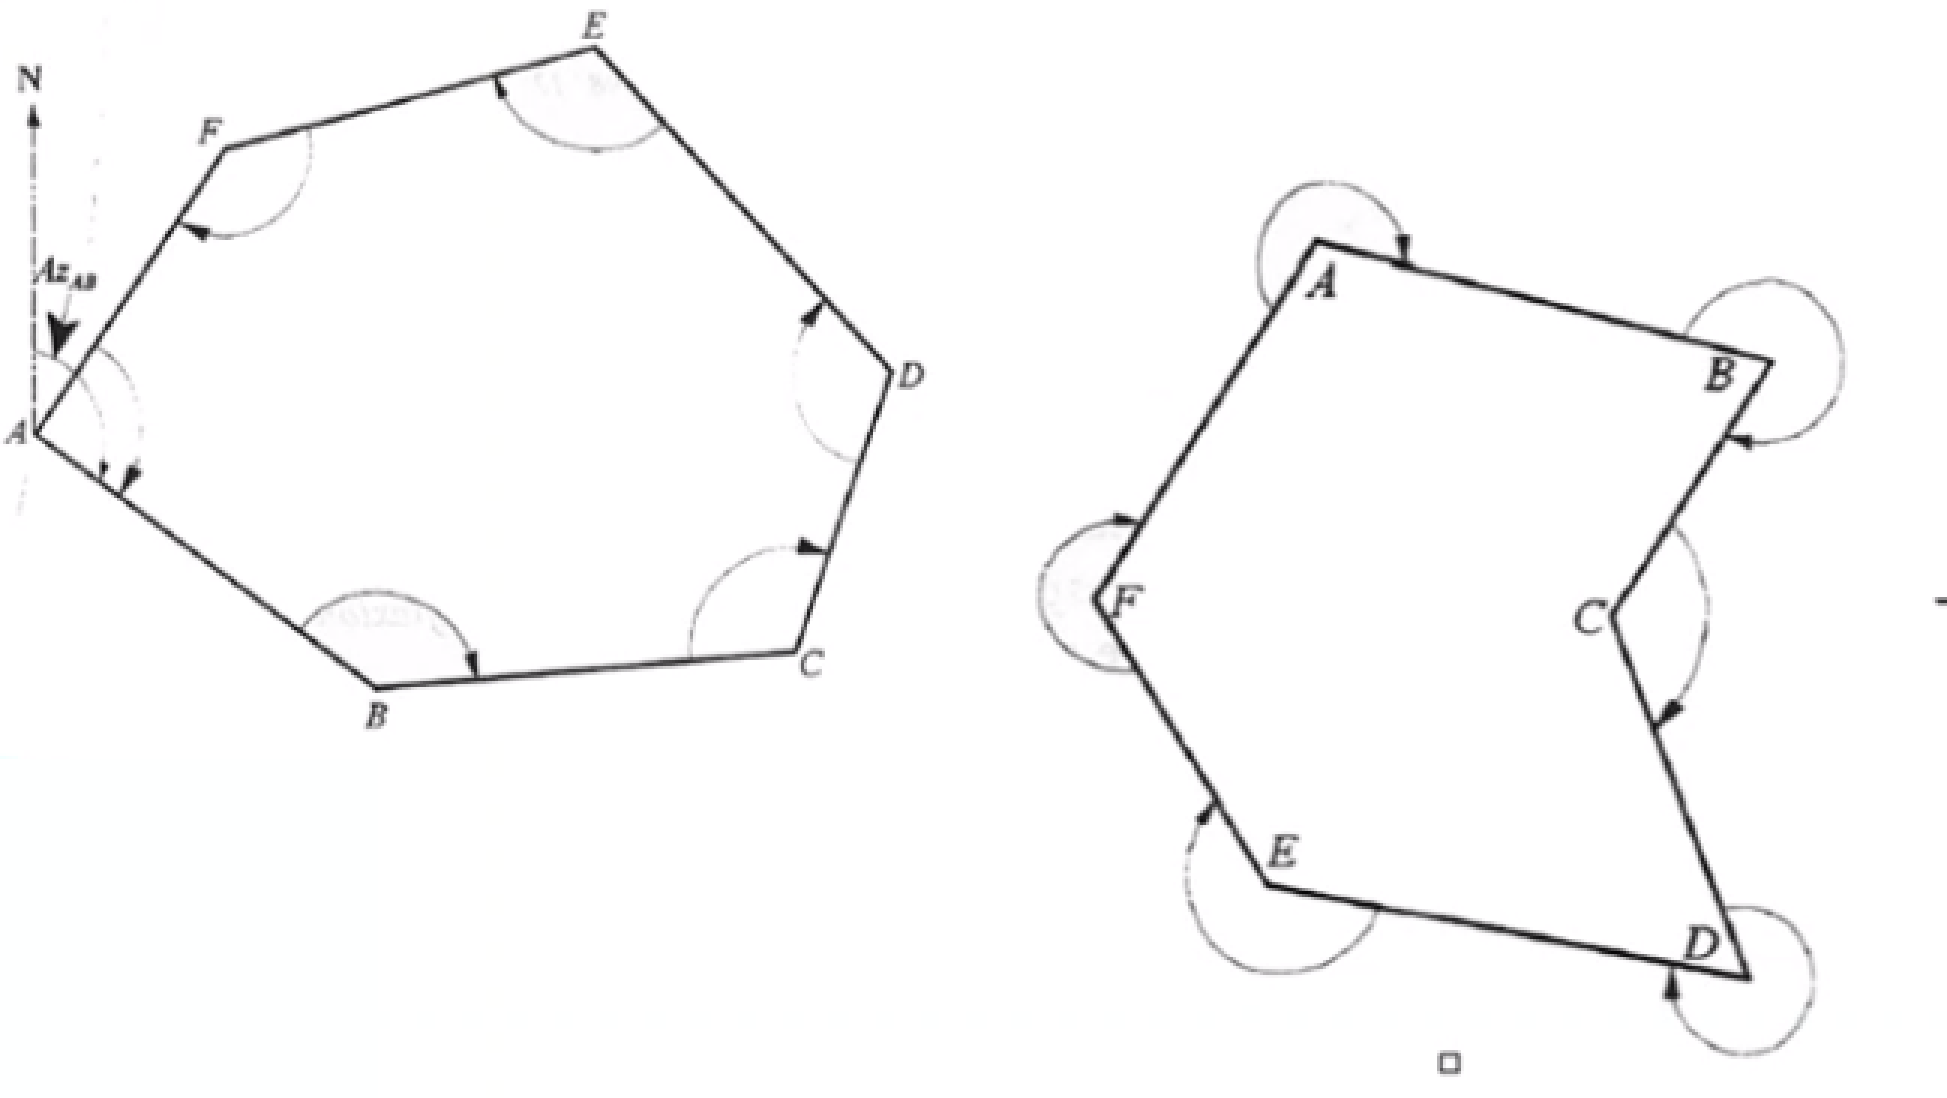
\includegraphics[width=\linewidth]{ta18.png}
    \caption{Medición de ángulos internos y externos para poligonales cerradas}
    \label{ta18}
    \end{subfigure}
    \begin{subfigure}[b]{0.45\linewidth}
    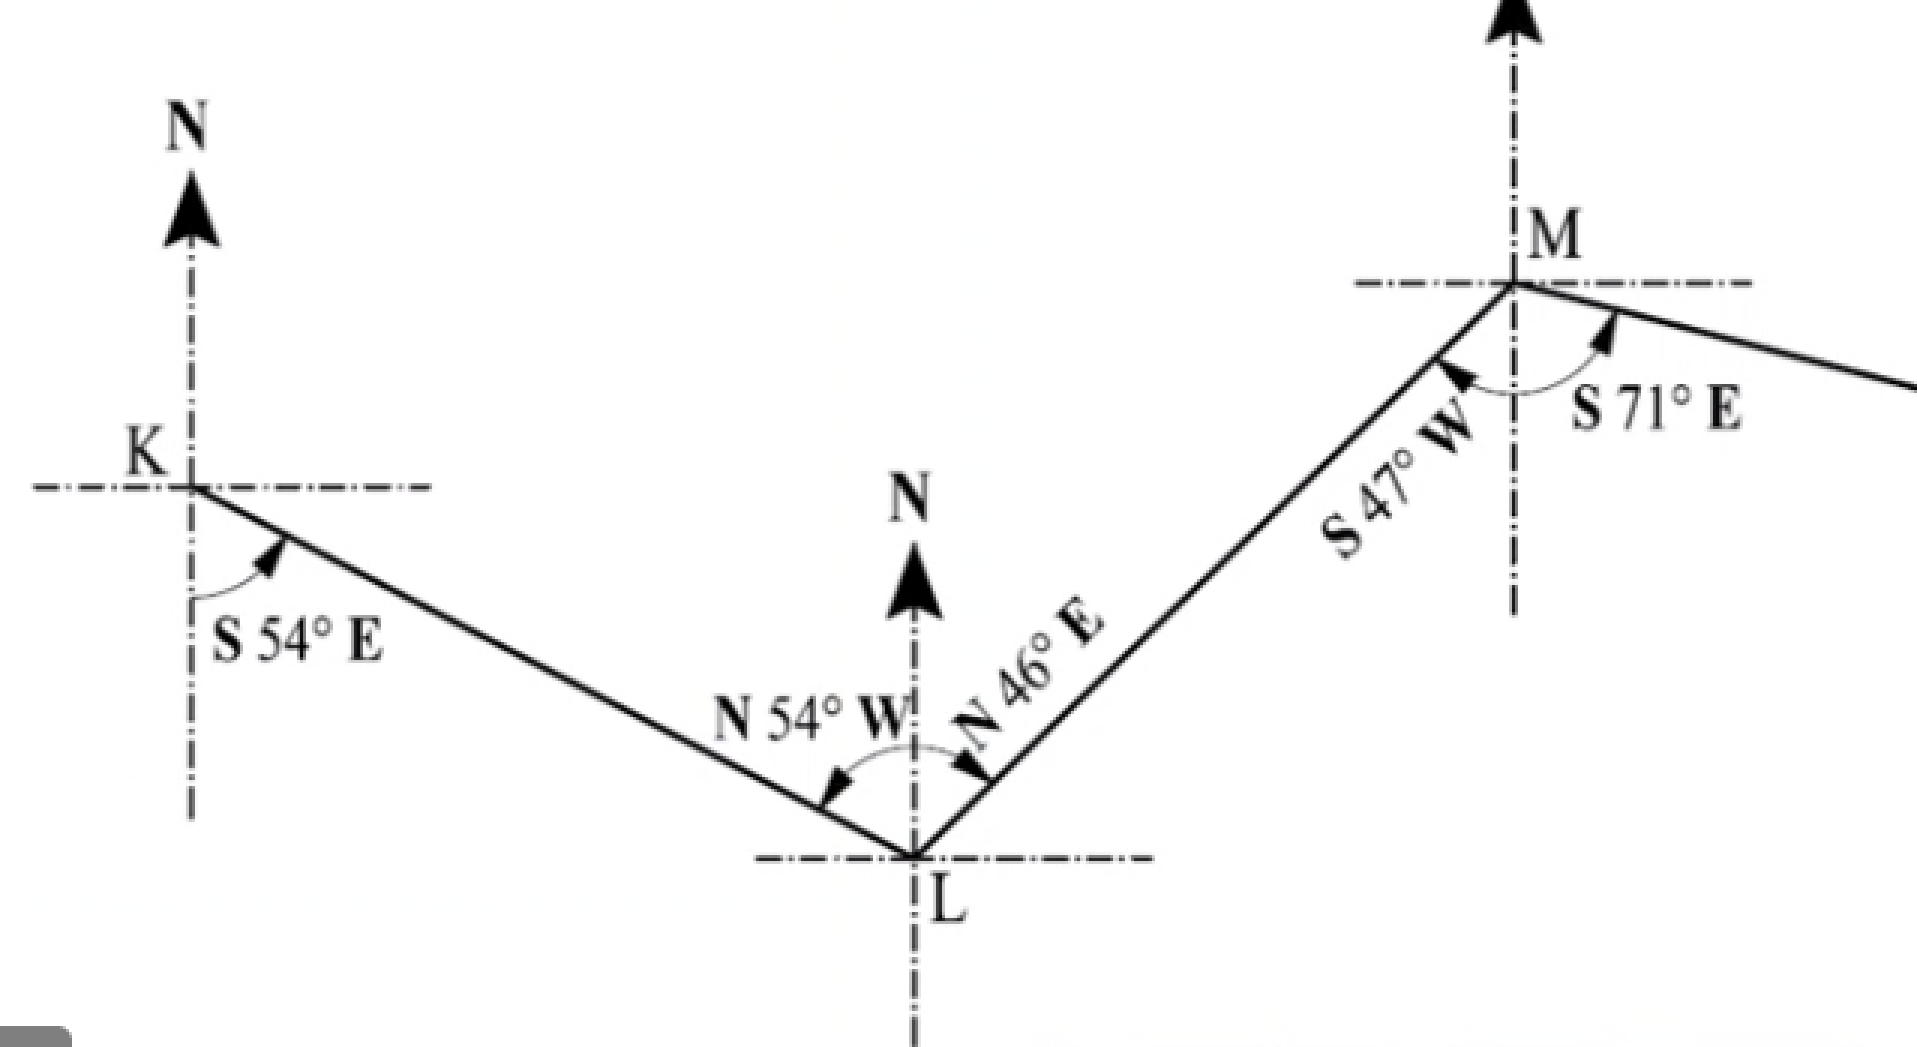
\includegraphics[width=\linewidth]{ta19.png}
    \caption{Medición de rumbos (a Azimuts). Para poligonales cerradas o abiertas}
    \label{ta19}
    \end{subfigure}
    \caption{Los primeros dos métodos de medición}
    \label{ta18-19}
\end{figure}

    \begin{figure}[h!]
        \centering
        \begin{subfigure}[b]{0.45\linewidth}
        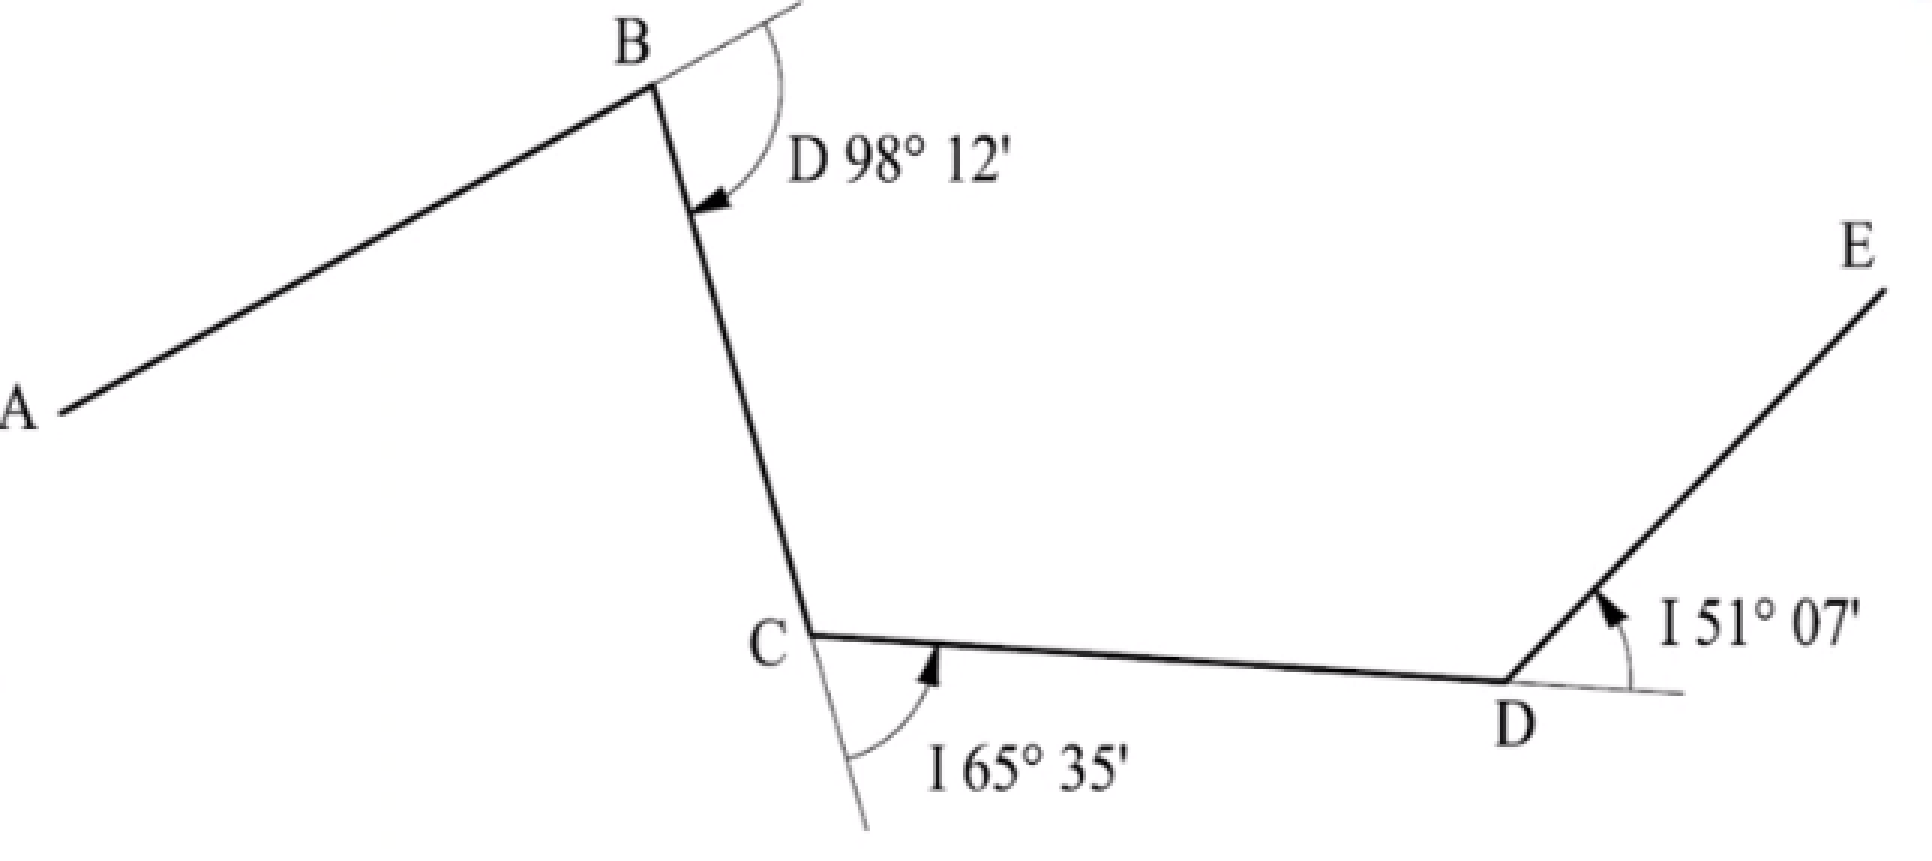
\includegraphics[width=\linewidth]{ta21.png}
        \caption{Medición  de ángulos de deflexión para poligonales abiertas}
        \label{ta20}
        \end{subfigure}
        \begin{subfigure}[b]{0.45\linewidth}
        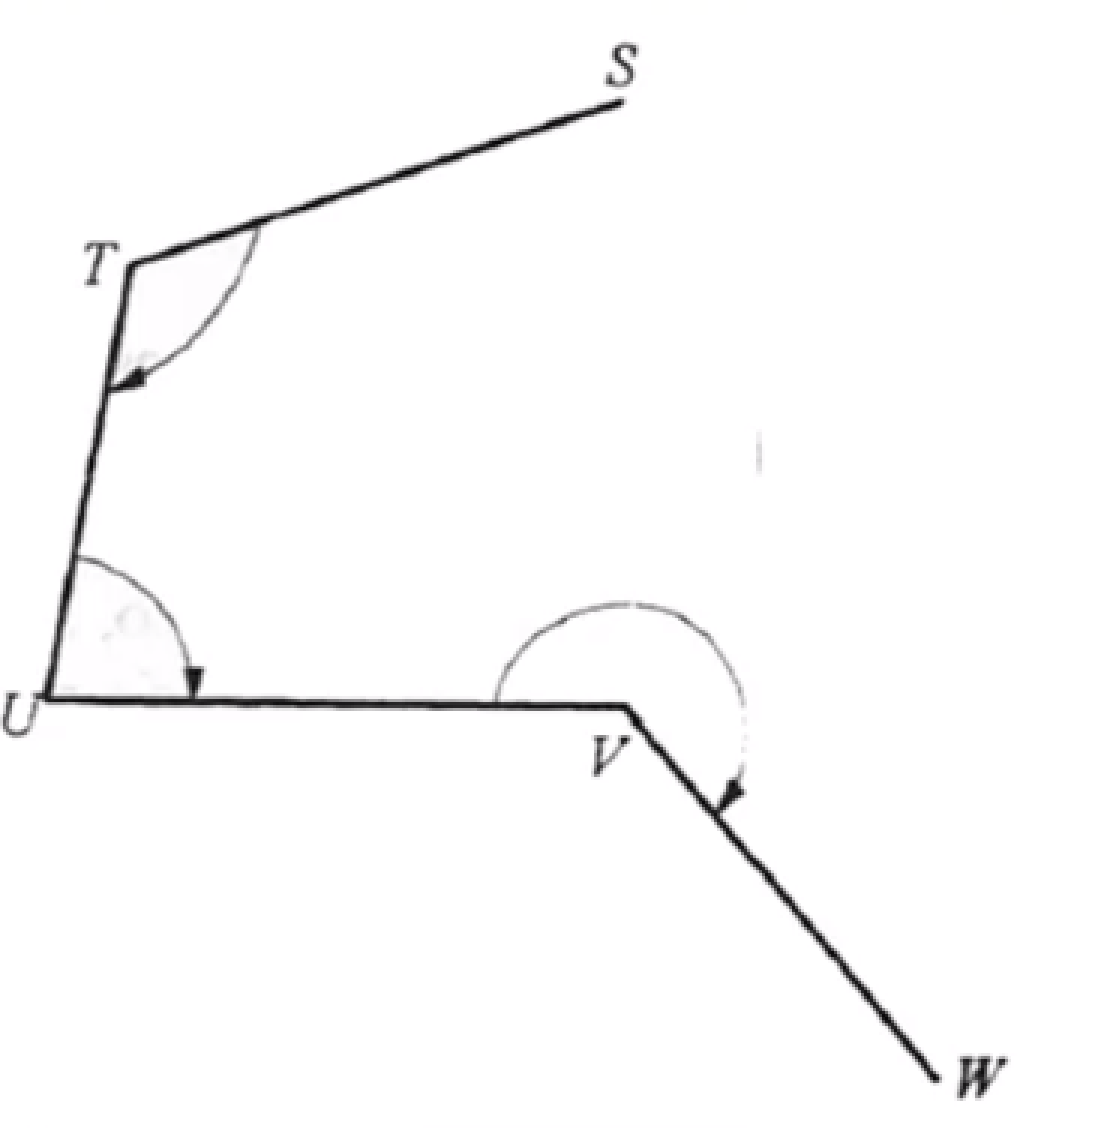
\includegraphics[width=\linewidth]{ta20.png}
        \caption{Medición de ángulos a la derecha (o al a izquierda) para ambos tipos de poligonal}
        \label{ta21}
        \end{subfigure}
        \caption{Los últimos dos métodos de medición}
        \label{ta20-21}
        \end{figure}


Sobre la medición de ángulos por el método de conversión de azimut.

Se usa la siguiente fórmula para el cálculo del azimut inverso de una línea.

\begin{equation}
    AzI_{AB}=Az_{BA}=AZ_{AB}\pm 180^{\circ}
\end{equation}

Se mide el azimut directo de la línea $RS$

\begin{equation*}
    AzD_{RS}=048^{\circ}15^{\prime}30^{\prime\prime}
\end{equation*}

Se calcula el azimut inverso de la línea $RS$ que corresponde el azimut directo de la línea $SR$ y se introduce en el instrumento estacionado en el $PCAS$ y visando el punto $R$:
\begin{align*}
    AzI_{RS}=AzD_{RS}+180^{\circ}=\left(048^{\circ}15^{\prime}30^{\prime\prime} \right)+180^{\circ}\\
    AzI_{RS}= 228^{\circ}15^{\prime}30^{\prime\prime}   
\end{align*}

Se mide el ángulo $AH$ en sentido horario en el punto $S$ al visitar el $PCA$ $T\left(263^{\circ}25^{\prime}54^{\prime\prime} \right)$ obteniéndose al azimut de la LCA $ST$
\begin{align*}
    AzD_{ST}=AzD_{RS}+AHS=AzF_{SR}= 228^{\circ}15^{\prime}30^{\prime\prime}+ 263^{\circ}25^{\prime}54^{\prime\prime}\\
    AzD_{ST}= gg^{\circ}15^{\prime}30^{\prime\prime}+ 263^{\circ}25^{\prime}54^{\prime\prime}= 491^{\circ}41^{\prime}24^{\prime\prime} \\
    AzD_{ST}= 131^{\circ}41^{\prime}24^{\prime\prime}
\end{align*}

\subsubsection{Cuadro de registro}

\textbf{Proyecto:} \underline{Vaso de almacenamiento de la presa de almacenamiento ``LAS TÓRTOLAS''}

\textbf{Procedimientos:} \underline{Poligonal cerrada}

\textbf{Instrumentos:} \underline{Teodolito de precisión y medidor electrónico de distancias (MED)}

\textbf{Medición angular:} \underline{Ángulos internos en sentido antihorario}

\textbf{Brigada:} \underline{Cuatro} \hfill \textbf{Fecha:} 24/09/2021


\begin{table}[h!]
    \centering
    \begin{tabular}{@{}ccccccc@{}}
    \toprule
    \multirow{2}{*}{Est} & \multirow{2}{*}{PV} & \multicolumn{3}{c}{AH}              & DH      & \multirow{2}{*}{Observaciones}                                        \\ \cmidrule(lr){3-6}
                         &                     & $\circ$ & $\prime$ & $\prime\prime$ & (m)     &                                                                       \\ \midrule
    A                    & B                   & 087     & 14       & 28             & 175.418 &                                                                       \\
    B                    & C                   & 198     & 42       & 15             & 283.172 & Terreno inestable                                                     \\
    C                    & D                   & 107     & 06       & 09             & 433.702 &                                                                       \\
    D                    & E                   & 090     & 13       & 46             & 461.085 &                                                                       \\
    E                    & F                   & 145     & 42       & 23             & 462.713 &                                                                       \\
    F                    & G                   & 052     & 57       & 09             & 309.801 & \begin{tabular}[c]{@{}c@{}}Problemas de \\ reverberancia\end{tabular} \\
    G                    & A                   & 218     & 00       & 56             &         &                                                                       \\ \bottomrule
    \end{tabular}
    \caption{Cuadro de registro}
    \label{tabta5}
\end{table}

\subsection{Nivelación de los PCA}

\begin{definition}[Nivelación]
Es el trabajo topográfico para determinar la coordenada $Z$ de los $PCA$ una vez establecidos en campo mediante cualquier procedimiento topográfico planimétrico y que se realiza siguiendo un procedimiento topográfico altimétrico
\end{definition}

La Board of Surveys and Maps del gobierno federal de EE.UU Clasifica la nivelación en cuatro grupos según su precisión.


\begin{definition}[Cota de un punto]
    También denotada como coordenada $Z$ es simplemente su elevación asignada o determinada sobre el plano de referencia elegido arbitrariamente
\end{definition}

Anteriormente era común, que la cota del primer punto usado como Banco de Nivel de un trabajo topográfico se asignará sin más consideración que asegurar que ningún punto del estudio resultará negativo

La nivelación diferencial es el procedimiento topográfico de altimetría que se emplea para la determinación de la coordenada $Z$ de puntos de control y apoyo

Consiste en emplear un nivel topográfico para generar un plano horizontal y se toman lecturas sobre estadales colocados sobre cada par de ellos, con cuya diferencia se obtiene el desnivel o proyección $Pz$

\begin{figure}[h!]
    \centerline{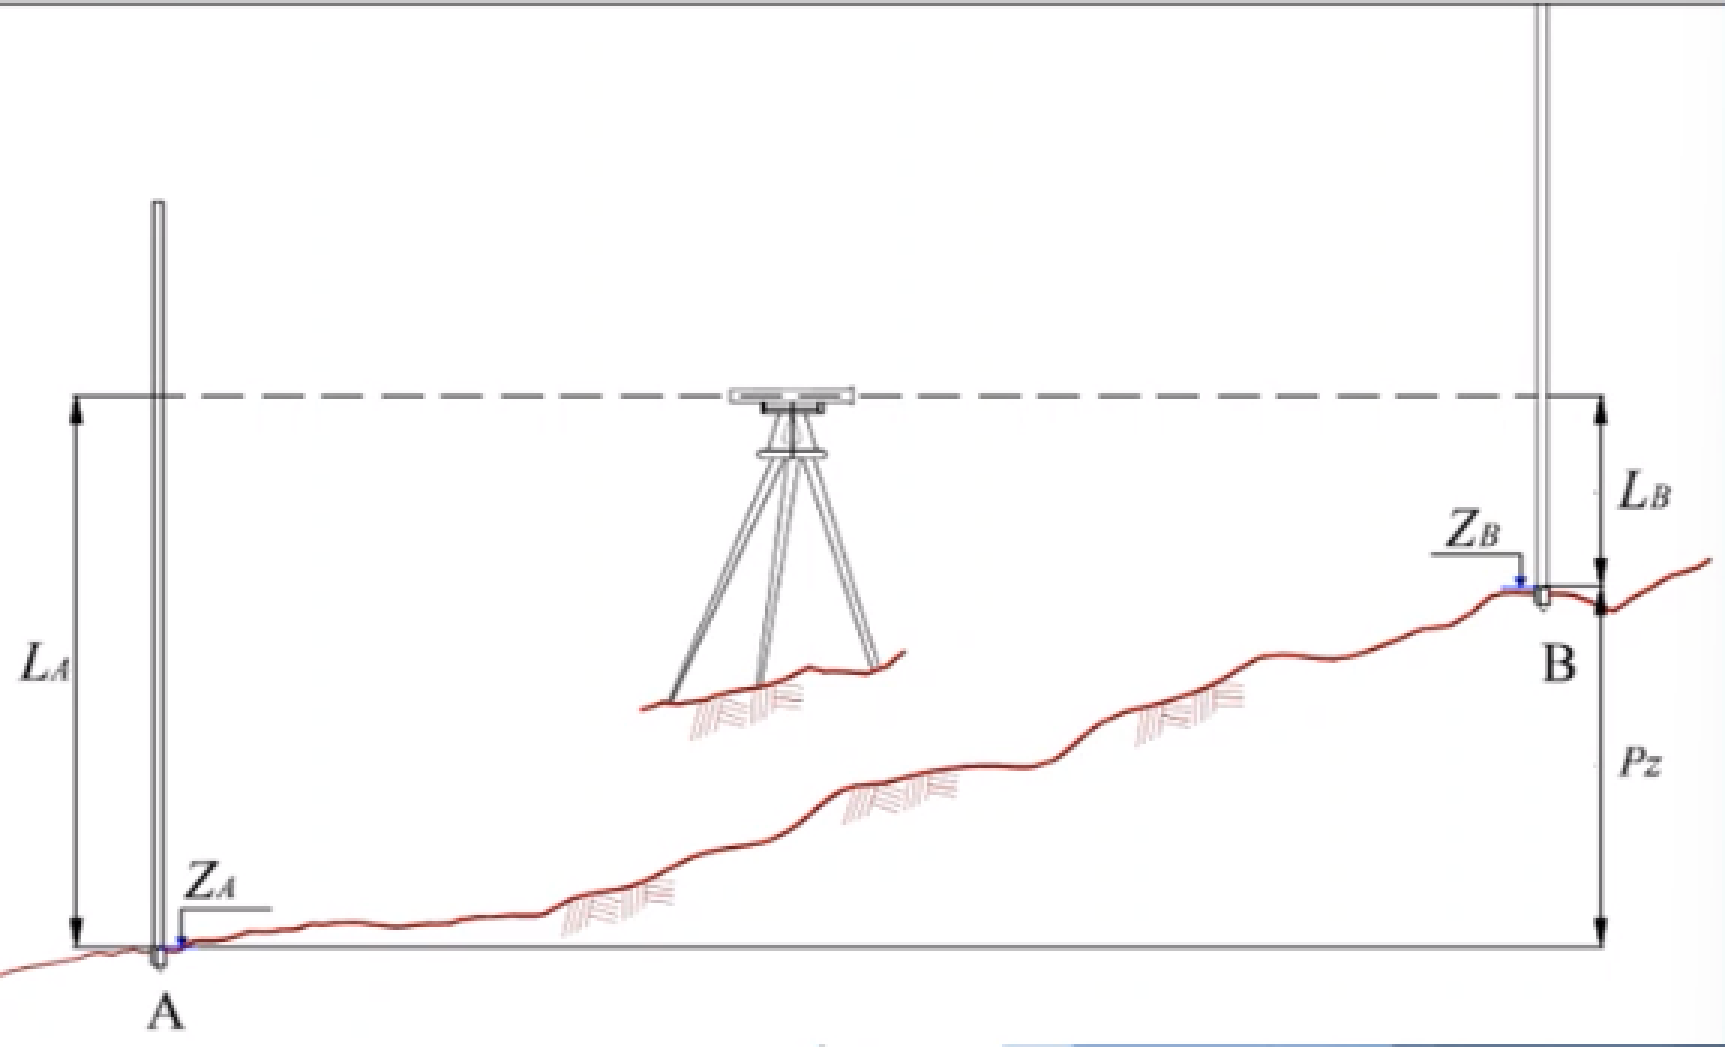
\includegraphics[width=0.5\textwidth]{ta23.png}}
    \caption{Nivelación diferencial}
    \label{ta23}
\end{figure}
\begin{align*}
    &Pz_{AB}=L_A-L_B&&Z_B=Z_A+Pz_{AB}&&Z_B=Z_A+(L_A-L_B)
\end{align*}

Elevación del instrumento: 
\begin{equation*}
    EI=Z_A+L_A=1935.418+3.192=1938.610
\end{equation*}
\begin{align*}
    &Z_A=1935.418m&&L_A=3.192m&&L_B=1.312m\\
    &Z_B=(1935.418)&&+3.192-1.312&&=1937.298m
\end{align*}

Cuando las lecturas en el estadal sobre los puntos A y B no se puede tomar simultáneamente desde el punto de ubicación del instrumento, ya sea porque Ay B estén muy alejados entre sí, o porque el desnivel entre ellos sea mayor que la longitud de los estadales, se presenta un problema que se resuelve mediante la nivelación diferencial compuesta

\begin{figure}[h!]
  \centerline{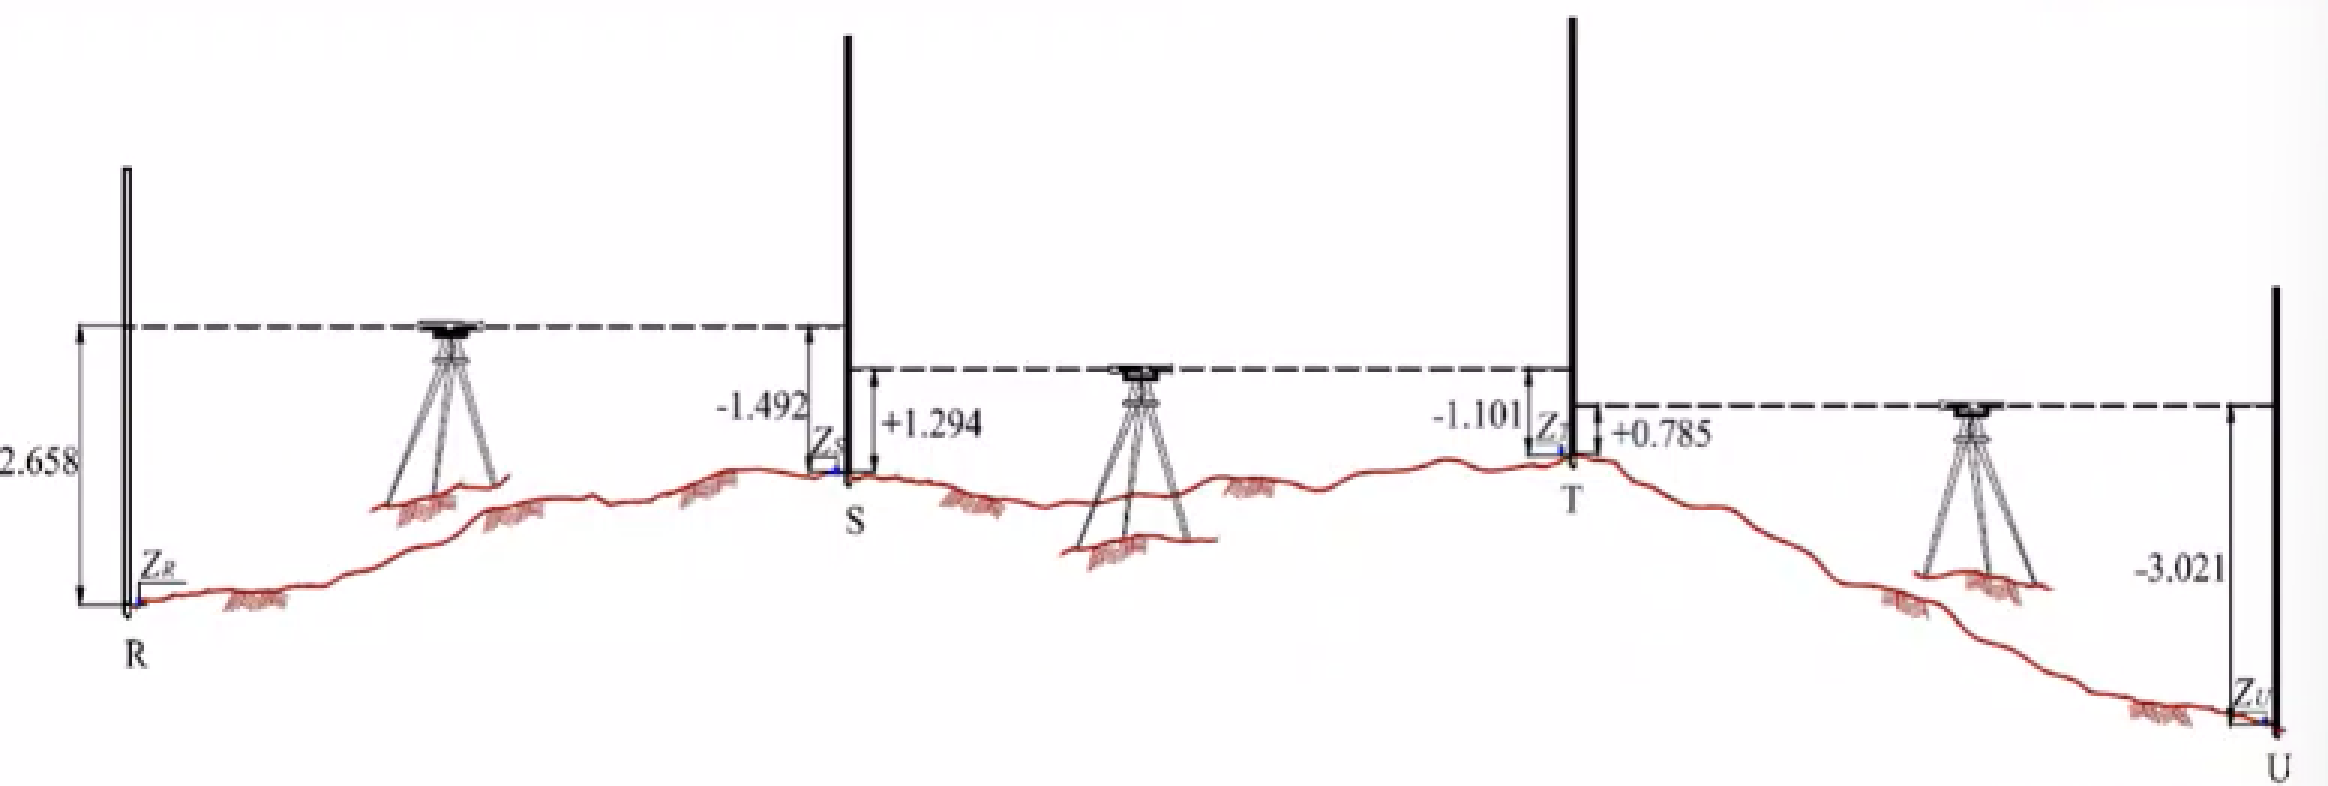
\includegraphics[width=0.5\textwidth]{ta24.png}}
  \caption{El instrumento se instala en el sitio más conveniente}
  \label{ta24}
\end{figure}
\begin{align*}
    EI_R=Z_R+L_R\\
    =1258.296+2.658=1260.954\\
    Z_s=EI_R-L_s\\
    =1260.954-1492=1259.462m
\end{align*}
\begin{table}[h!]
    \centering\begin{tabular}{@{}ccccc@{}}
    \toprule
    \multirow{2}{*}{PV} & LP    & EI       & LN    & $Z_r$     \\ \cmidrule(l){2-5} 
                        & (m)   & (m)      & (m)   & (m)       \\ \midrule
    R                   & 2.658 & 1260.954 &       & 1258.296 \\
    S                   & 1.294 & 1260.756 & 1.492 & 1259.462  \\
    T                   & 0.785 & 1260.440 & 1.101 & 1259.655  \\
    U                   & 3.152 & 1263.723 & 3.021 & 1257.419  \\
    V                   & 2.896 & 1263.767 & 2.852 & 1260.871  \\
    W                   &       &          & 3.659 & 1260.108  \\ \bottomrule
    \end{tabular}
    \caption{Cuadro de registro y cálculo de cotas}
    \label{tabta6}
\end{table}

\subsubsection{Nivelación diferencial por el método de los tres hilos}

Las distancias se calculan con la fórmula de \texttt{estadia simple}

\begin{equation}
    DH=100\left(LHS-LHI\right)
\end{equation}

\begin{figure}[h!]
  \centerline{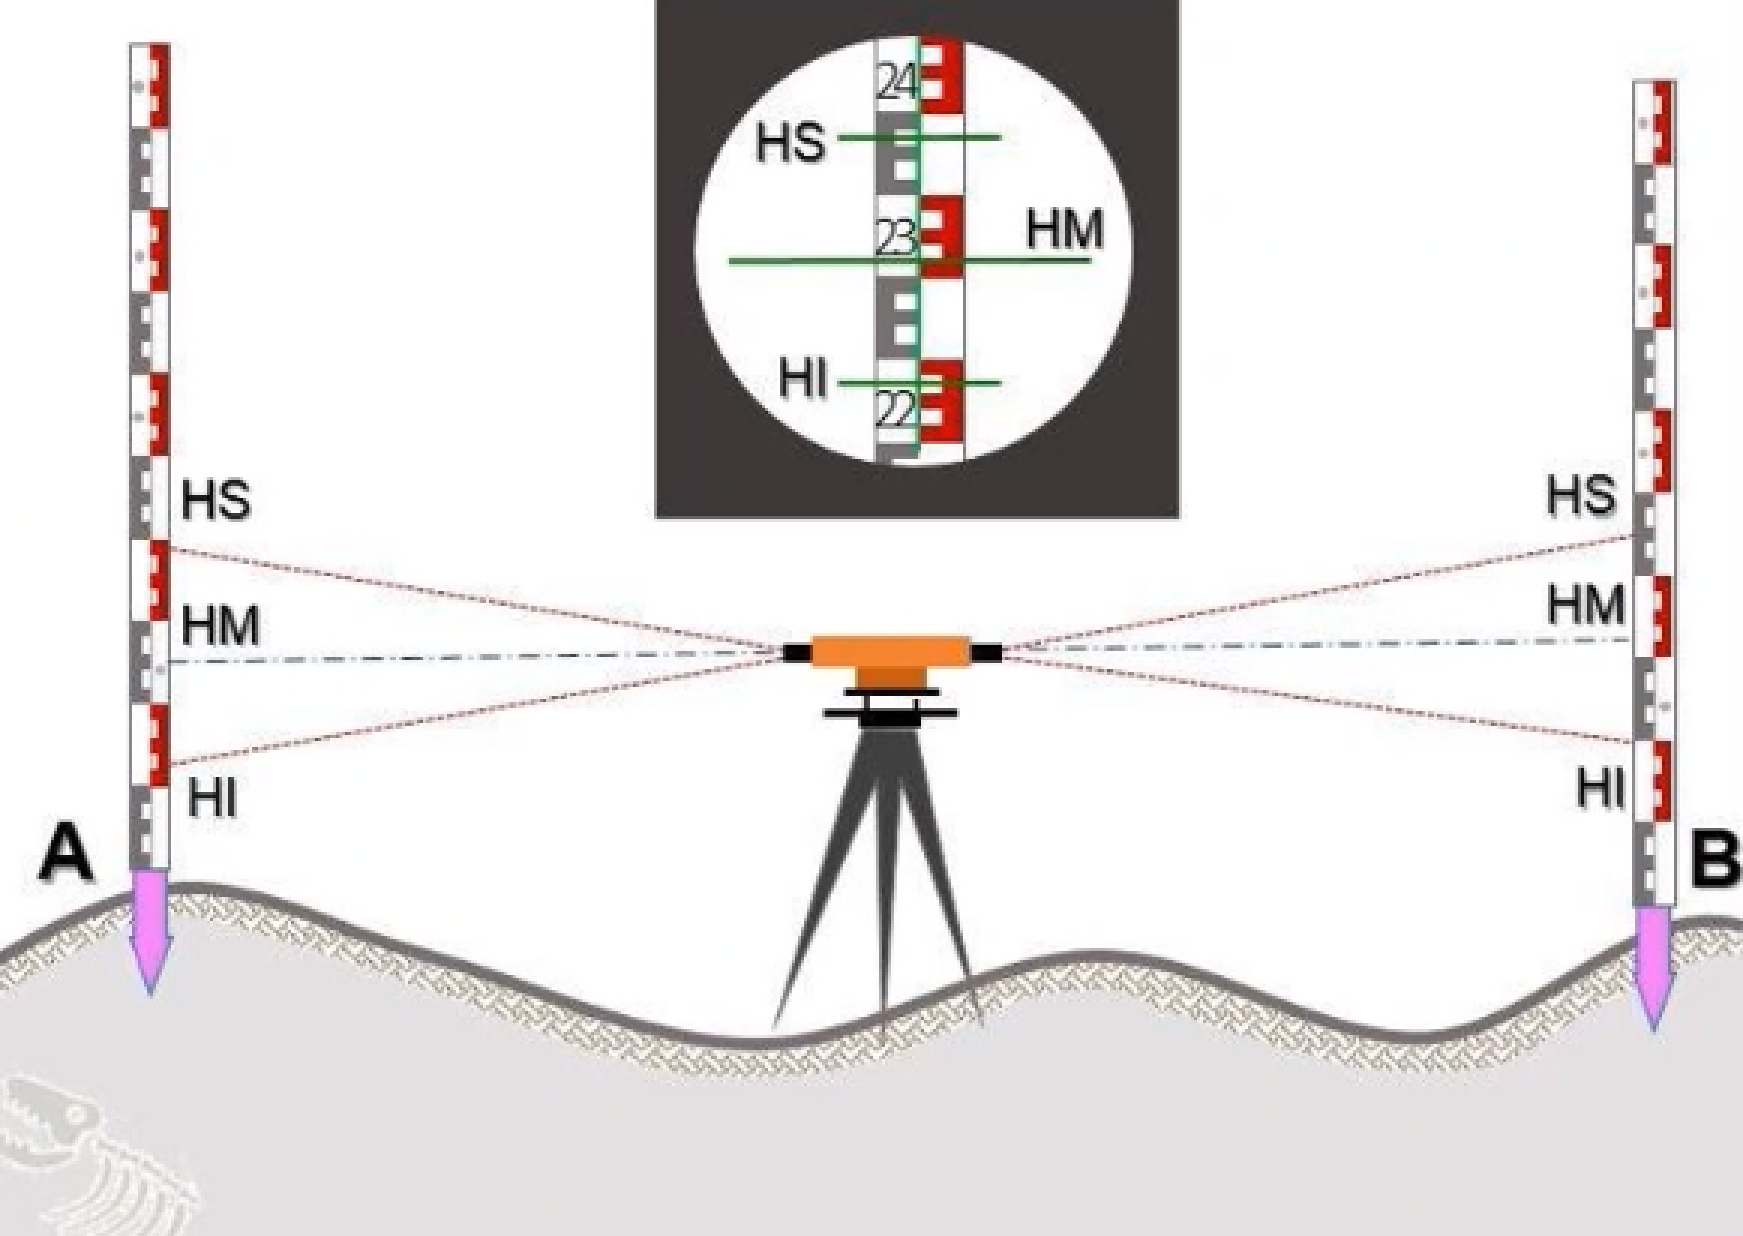
\includegraphics[width=0.5\textwidth]{ta25.png}}
  \caption{Nivelación diferencial por el método de los tres hilos}
  \label{ta25}
\end{figure}

\begin{figure}[h!]
  \centerline{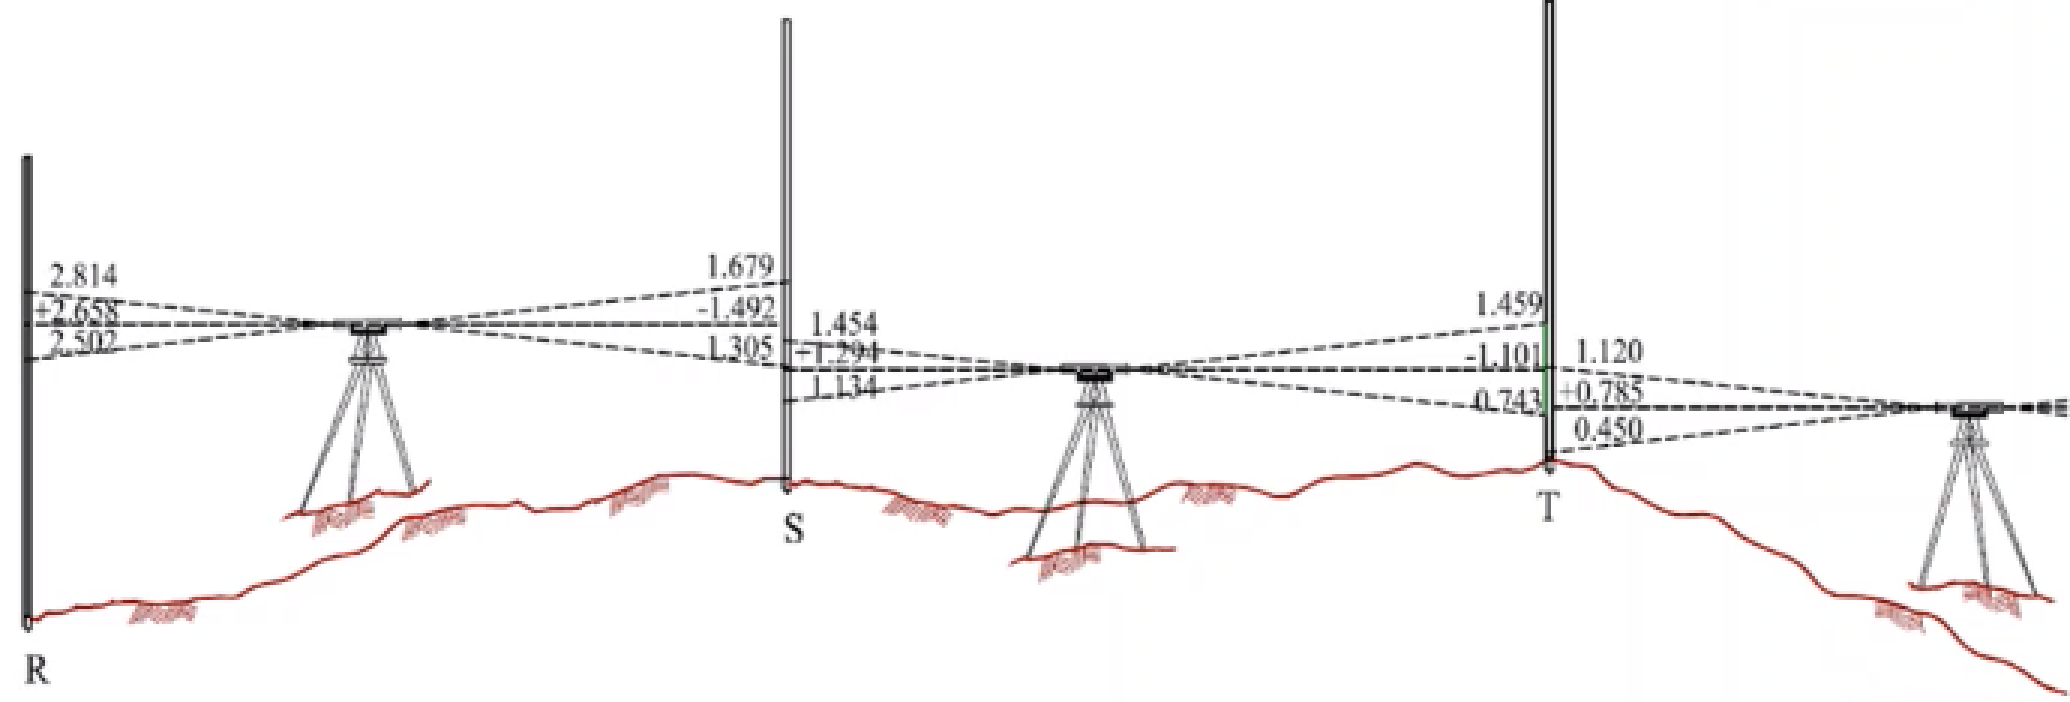
\includegraphics[width=0.5\textwidth]{ta26.png}}
  \caption{Medición}
  \label{ta26}
\end{figure}

\begin{table}[h!]
    \centering\begin{tabular}{@{}ccccccccccc@{}}
    \toprule
    \multirow{3}{*}{PV} & \multirow{2}{*}{LP} & \multirow{2}{*}{AI} & \multirow{2}{*}{LN} & \multirow{2}{*}{Z} & \multicolumn{3}{c}{Hacia adelante} & \multicolumn{3}{c}{´Hacia atrás} \\
                        &                     &                     &                     &                    & LHS       & LHI       & DH         & LHS       & LHI      & SH        \\
                        & (m)                 & (m)                 & (m)                 & (m)                & (m)       & (m)       & (m)        & (m)       & (m)      & (m)       \\ \midrule
    R                   & 2.659               & 102.658             &                     & 100.000            &           &           &            & 2.814     & 2.502    & 31.200    \\
    S                   & 1.294               & 102.460             & 1.492               & 101.166            & 1.679     & 1.305     & 37.400     & 1.454     & 1.134    & 32.000    \\
    T                   & 0.785               &                     & 1.101               & 101.359            & 1.459     & 0.743     & 71.600     & 1.120     & 0.450    & 67.000    \\ \bottomrule
    \end{tabular}
    \caption{Cuadro de registro para la nivelación diferencial por el método de tres hilos}
    \label{tabta7}
\end{table}

\subsection{Estudio de los errores o (error y tolerancia)}

Los errores cometidos, son muy importantes y tiene que ser considerados, evaluados y compensados, pueden tener diversas causas y orígenes

\begin{example}
    \textbf{Los errores Naturales:} Se originan por efecto de los elementos o factores del clima en los instrumentos o en las mediciones por la dilatación por temperatura, reverberancia por calor, catenaria por gravedad o inestabilidad del viento
\end{example}

\begin{example}
    \textbf{Error instrumental:} Se deben a la deficiente construcción de los instrumentos o al desajuste de sus partes móviles, por una mala graduación de una cinta, o desajuste del nivel del tránsito
\end{example}

\begin{example}
    \textbf{Error personal:} Se deben al desconocimiento, falta de atención, por una mala operación de los equipos, incorrecta lectura o anotación de datos
\end{example}

\begin{example}
    \textbf{Sistemáticos:} Siguen leyes físicas o matemáticas, por tanto, se puede calcular y corregir; siempre son del mismo, Por Cuaternaria puede ser:
    \begin{equation}
        E_c=\frac{Wc^2\times Lm^3}{24t^2}
    \end{equation}
    Por dilatación por temperatura: 
    \begin{equation}
        Ed=\alpha_mLM(T-T_0)
    \end{equation}
\end{example}

\begin{example}
    \textbf{Gruesos o equivocaciones:} No siguen ninguna ley, hay mala operación de los equipos, incorrecta lectura o anotación de datos.
\end{example}

\begin{example}
    \textbf{Aleatorios o accidentales:} Siguen las leyes de la probabilidad y la estadística y es igualmente probable que sean positivos o negativos. Se distribuyen entre los valores medidos siguiendo criterios que contemplen las condiciones de medición.
\end{example}

\begin{definition}[Error (E)]
    Es la diferencia algebraica entre el valor observado o medido ($V_0$) y el valor verdadero $V_v$ o más probable $V_p$ de una magnitud cualquiera
\end{definition}
Cuando una magnitud se mide varias veces en las mismas condiciones, el mejor estimado del valor verdadero es la media aritmética $V$

\begin{equation}
    V=\frac{1}{n}\sum_{i=1}^n VO_i=\frac{VO_1+VO_2+VO_+\dots+VO_n}{n}\mid E=VO-V
\end{equation}

\begin{definition}[Error total (ET)]
    Es la suma algebraica de todos los errores accidentales cometidos al efectuar una medición (pueden tener signos positivos o negativos)
\end{definition}
\begin{equation}
    E=VO-Vv=VO-VP
\end{equation}

\begin{table}[h!]
    \centering\begin{tabular}{|c|c|c|}
    \hline
    $(i)$   & $V_{Oi}$ & $E_i$          \\ \hline
    1       & $V_{O1}$ & $R_1=V_{O1}-V$ \\ \hline
    2       & $V_{O1}$ & $R_1=V_{O1}-V$ \\ \hline
    3       & $V_{O1}$ & $R_1=V_{O1}-V$ \\ \hline
    $\vdots$& $\vdots$ & $\vdots$       \\ \hline
    n       & $V_{O1}$ & $R_1=V_{O1}-V$ \\ \hline
    \end{tabular}
    \caption{La fórmula dada $ET=\sum_{i=1}^n E_i$ define el error total}
    \label{tabta8}
    \end{table}

Como son errores accidentales, se distribuyen siguiendo la distribución normal o ley de distribución de los errores

la media aritmética del error no es conveniente porque tiene que ser cero
\begin{align*}
    &\text{Varianza}&&EMC=\frac{ETC}{n}\\
    &\text{Error total cuadrático}&&ETC=n\times EMC\\ 
    &\text{Error estándar}&&EE=\sqrt{EM}\\
    &\text{Error residual}&&ET^2=ETC\\
    &\text{Error estándar}&&ER=\sqrt{ETC}\\
    &\text{Erorr máximo}&&ER=\pm\sqrt{n}\times EE
\end{align*}

\begin{definition}[Exactitud]
    Se presenta cuando se obtiene el valor sin ningún error
\end{definition}

\begin{definition}[Precisión]
    En el grado de aproximación a dicho valor verdadero, en general la precisión $Pr$ se puede calcular como una fracción respecto de 1: 
\end{definition}
\begin{equation}
    Pr=\frac{V_v}{E}=\frac{1}{\frac{E}{V_v}}
\end{equation}

El error máximo positivo o negativo que se está dispuesto a aceptar en una medición y que por lo tanto sirve como criterio de decisión. En la práctica, es muy común considerar a la tolerancia como el doble del error residual
\begin{equation}
    T=2\times ER=\pm 2\sqrt{n}\times EE
\end{equation}
Aplica para errores accidentales.

Si $E<T$ el trabajo se acepta, la tolerancia depende del tipo de medición:

\begin{itemize}
    \item Las mediciones lineales deben ser unitarias
    \item Las mediciones angulares deben ser totales
\end{itemize}


Para el cierre angular de una poligonal cerrada de precisión $EE=\pm a/2$

\begin{equation}
    Ta=\pm a\sqrt{n}
\end{equation}


\subsection{Comprobación y compensación de una poligonal cerrada}

Condición de cierre angular, se midan los ángulos internos AI para el cálculo del error angular EA:
\begin{equation*}
    \sum_{i=0}^nAI_i=180(n-2)\implies EA=\sum_{i=1}^nAI_i-180(n-2)
\end{equation*}
Si se miden los ángulos externos $AE:$

\begin{equation*}
    \sum_{i=1}^nAE_i=180(n-2)\implies EA=\sum_{i=1}^nAE_i-180(n+2)
\end{equation*}

Hay una condición de cierre lineal: La suma algebraica de las proyecciones de todos sus lados sobre los ejes de un sistema coordenado rectangular, debe ser igual a cero: 
\begin{align*}
    &\sum_{i=1}^nPx_i=0\\
    &\sum_{i=1}^nPy_i=0
\end{align*}

Cálculo del error lineal:
\begin{align*}
    &\text{Error en la dirección }x&&\text{Error en la dirección }x&&\text{Error en la dirección }x\\
    &EX=\sum_{i=1}^nPx_i&&Ey=\sum_{i=1}^nPy_i&&EL=\sqrt{Ex^2+Ey^2}
\end{align*}

El error unitario EY es el error por unidad de longitud:
\begin{align}
    &EU=\frac{EL}{LT}\\
    &LT=\sum_{i=1}^nL_i
\end{align}

LT= Longitud total de la poligonal.

Para calcular las proyecciones, se realiza:
\begin{align}
    &Px_i=L_i\left(\sin{(Az_i)}\right)\\
    &Py_i=L_i\left(\cos{(Az_i)}\right)
\end{align}

Primero se calcula el error, después la comparación con la tolerancia para aceptar el trabajo para compensarlo.
\begin{enumerate}
    \item Repartir el error angular por igual entre todos y cada uno de los ángulos medidos: En el primer caso, se parte del supuesto de que todos los ángulos fueron medidos en igualdad de condiciones, respecto a los instrumentos utilizados, al personal que lo realizó y a las condiciones naturales prevalecientes durante su realización y por lo tanto se les atribuye el mismo grado de confianza o de confiabilidad y de probabilidad de error.
    \item Repartir el error angular de acuerdo con algunas consideraciones respecto a la confiabilidad de cada una de las mediciones: Por ejemplo: si algunos ángulos fueron medidos con un instrumento de mayor precisión, se las atribuirá mayor confiabilidad y se les afectará con menor o nulo valor de corrección; cuando una magnitud angular se determina con una serie de reparticiones, se le puede atribuir mayor precisión y confianza; en condiciones ambientales desfavorables como fuertes vientos, reverberancias o neblina, o en donde los suelos son inestables, las lecturas serán seguramente menos confiables.
\end{enumerate}

\subsubsection{Regla de tránsito}
Se supone que las mediciones angulares son más precisas que las lineales, lo que implica darle un mayor grado de confianza a las primeras y las correcciones a las proyecciones se calculan proporcionalmente a los valores angulares.
Para la dirección $x$:

\begin{equation}
    Cx_i=-Ex_i=-\frac{Ey_i}{\sum_{i=1}^n\left\lvert Px_i\right\rvert}\left\lvert Px_i\right\rvert 
\end{equation}
Para la dirección $y$:
\begin{equation}
    Cy_i=-Ex_i=-\frac{Ey_i}{\sum_{i=1}^n\left\lvert Py_i\right\rvert}\left\lvert Py_i\right\rvert
\end{equation}

$Cx_i$ es la corrección en la dirección $x$ de la lineal $i$, ambas correcciones son contrarias en signos a sus respectivos errores


\subsection{Comprobación y compensación ordinaria de nivelación}

Fórmula para calcular la tolerancia de nivelación en cm:

\begin{equation}
    T=Tz=a\sqrt{K}
\end{equation}

$K$ es la longitud del recorrido total de la nivelación en km; $a$ es un factor que depende de la precisión requerida y de las condiciones de operación en campo y cuyo valor debe ser teóricamente el doble del error estándar.

\begin{itemize}
    \item Primer orden, a=4.2
    \item Segundo orden a=8.4
    \item Tercer orden a=12.6
    \item Cuarto orden a=16.8
\end{itemize}

Casos para la comprobación: Establecimiento de un nuevo PCA  a partir de otro previamente definido y/o establecimiento de varios PCA intermedios entre dos previamente definidos.


Nivelación de Ida y Regreso. Consiste en partir del PCA cuya coordenada $Z$ se conoce, hacer la nivelación por nivelación diferencial, colocando tantos puntos de liga (PL)
como sean necesarios y llegar al PCA final cuya coordenada $Z$ se desea determinar, y repetir el proceso de nivelación ubicando nuevamente los $PL$ necesarios (pero diferentes a los del proceso de ida), regresando al PCA inicial para comprobar el trabajo

\begin{equation}
    EN=Ez=ZN_A-ZV_A
\end{equation}

La corrección del error se hace como sigue:

\begin{align}
    &Cz=-\frac{Ez}{2}\\
    &ZC_B=ZN_B+Cz_B
\end{align}

\subsubsection{Nivelación don doble punto de liga}

Constituye en realidad, una doble Nivelación (y por lo tanto, se recomienda llevar un cuadro de registro para cada proceso), ya que se ubica un doble número de puntos de liga y se toman lecturas sobre el estadal colocados en ellos, desde cada puesta del instrumento de nivelación de manera que al llegar al nuevo PCA(B) se obtienen dos coordenadas calculadas con el proceso de nivelación distintas en general $ZN_{Bi}$ y $ZN_{B2}$

El error de nivelación total es:
\begin{equation}
    EN=Ez=ZN_{B1}-\frac{ZN_{B1}+ZN_{B2}}{2}
\end{equation}
Las correcciones del error se hace como sigue:
\begin{align}
    Cz=-Ez\\
    zC_B= \frac{ZN_{B1}+ZN_{B2}}{2}
\end{align}

\subsubsection{Nivelación con doble altura del apartado}

Este caso de comprobación es muy similar al anterior, pues éste se realizan también dos procesos de nivelación simultáneos, se llevan dos registros y se obtienen dos coordenadas $Z$ para el punto $B$; la única diferencia es que, en esta forma de comprobación, se toman dos lecturas para un mismo punto de liga desde dos puestas.\footnote{Las fórmulas son las mismas que las anteriores.}

Criterios para distribuir el error.
\begin{enumerate}
    \item El error de nivelación $Ez$ se distribuye entre todos los PCA intermedios, proporcionalmente a las distancias recorridas
    \begin{equation}
        \frac{Ez_i}{DN_i}= \frac{Ez}{Dt}
    \end{equation}

    \item El error de nivelación $Ez$, se distribuye entre todos los PCA intermedios, proporcionalmente los desniveles en los PCA nivelación 
    \begin{equation}
        \frac{Ez_i}{\left\lvert Pz_i\right\rvert }=\frac{Ez}{\sum_{i=1}^n\left\lvert Pz_i0\right\rvert }
    \end{equation}
    \item Distribuir el error $Ez$ proporcionalmente al número de puntos de liga que se establecieron entre cada par de PCA nivelados consecutivos
    \begin{equation}
        Cz_i=-Ez_i=-\frac{Ez}{Dt}DN_i
    \end{equation}
\end{enumerate}

\subsection{Levantamiento para configuración y de detalles}

La configuración de un terreno, es la representación planialtimétrica de éste, a base de curvas de nivel con las que se dibuja y visualiza su relieve en un plano y, al trabajo de campo que consiste en el  levantamiento o captura de la información necesaria, para ello se denomina levantamiento para configuración o de relleno y se hace aplicando alguno o una combinación de los métodos topográficos.

Con toda seguridad, un plano mostrando la configuración del terreno con curvas de nivel equidistantes verticalmente, es la máxima expresión gráfica del mismo.

Los planos de configuración mediante el análisis de las curvas de nivel y si correcta interpretación, deben permitir una completa idea del relieve del terreno, e incluso la determinación del desnivel y la pendiente entre cualquier par de puntos y obtener un perfil de su terreno sobre un trazo en cualquier dirección

Para obtener la configuración de un terreno, es requisito indispensable conocer la posición en planta y elevación (preferentemente mediante sus coordenadas, como se ha insistido) de un número suficiente de puntos del terreno, distribuidos que se denominan Puntos para Configuración.

La cantidad de puntos de posición conocida, que se requieren para una buena configuración, depende de la precisión o detalle requeridos en el dibujo (según su finalidad) y del relieve del terreno definido por la conformación y variabilidad de las pendientes (suaves, abruptas, irregulares, uniformes, etc.)

En cuanto a la ubicación y distribución de los puntos, debe definirse de tal manera que su cantidad y localización debe implicar que sean más representativos posible del terreno, capturando puntos clave del terreno, que definan los cambios de pendiente, como son los que determinan las líneas de corriente de la red de drenaje y los parteaguas, así como todos los accidentes topográficos notables tales como altos y bajos.

Para complementar la información que se debe registrar en los planos, comúnmente se requieren registrar y por lo tanto, levantar detalles del terreno tales como linderos, vías de comunicación, infraestructura hidráulica, construcciones, etc. que son los Puntos de Detalle.

Ecuaciones para el cálculo de coordenadas de los PCD

\begin{align}
    &DH_{EP}=100\cdot \left(LHS-LHI\right)\cos^2{(AL_v)}\\
    &DH_{EP}=100\cdot (LHS-LHI)\sin^2{(AZ_v)}\\
    &Pz_{EP}=hi+50\cdot (LHS-LHI)\sin{(2AL_v)}-LHM\\
    &Pz_{EP}=hi+50\cdot (LHS-LHI)\sin{(2AZ_v)}-LHM\\
    &D_v=50\cdot (LHS-LHI)\sin{(2AL_{EP})}\\ 
    &Az_{EP}=Az_{LR}+AH_v
\end{align}
\begin{align}
    &Pz_{EP}=DI_{EP}\cdot \sin{(AL_{EP})}&&Px_{EP}=DH_{EP}\cdot \sin{(AZ_{EO})}\\
    &Pz_{EP}=DI_{EP}\cdot \cos{(AZ_{EP})}&&Py_{EP}=DH_{EP}\cdot Az_{EP}
\end{align}
El trabajo de gabinete está esquematizada en la figura \ref{ta27} por éstas igualdades: 

\begin{figure}[h!]
    \centerline{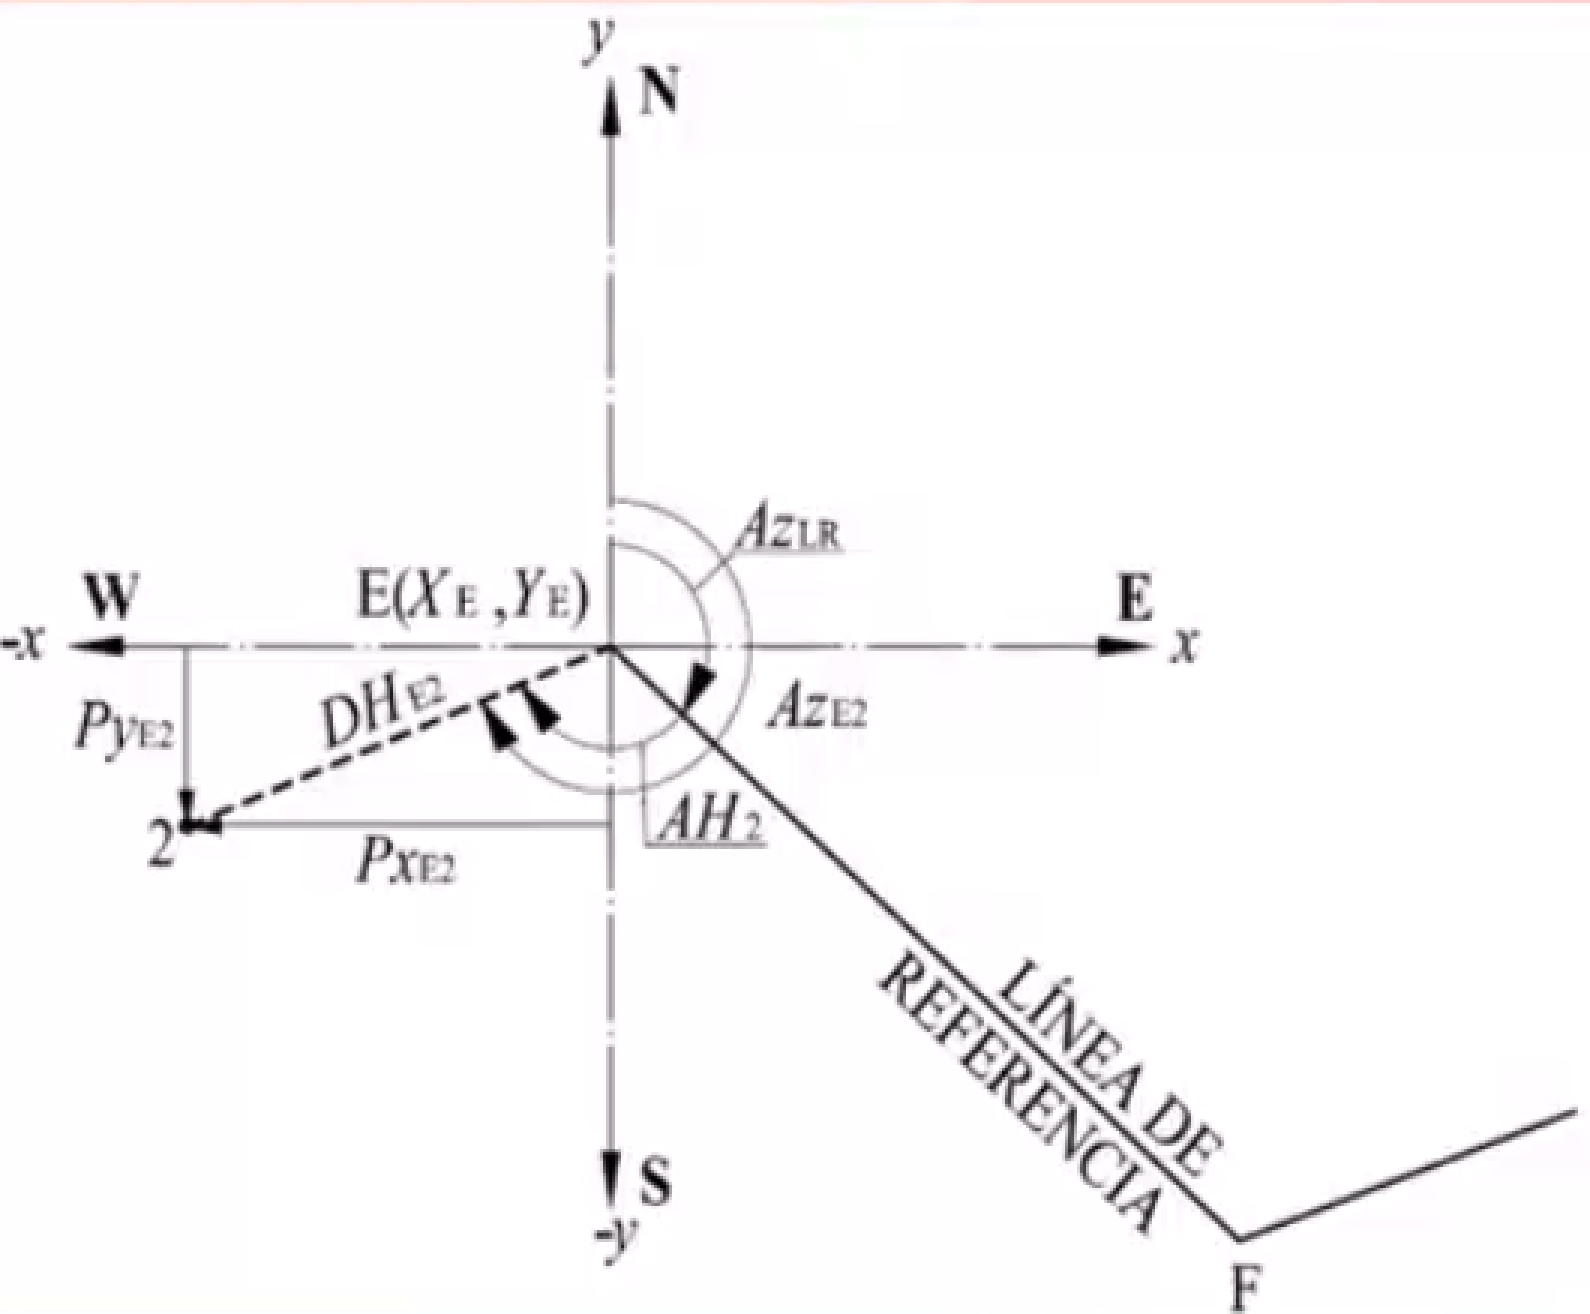
\includegraphics[width=0.5\textwidth]{ta27.png}}
    \caption{Trabajo de gabinete}
    \label{ta27}
\end{figure}

\begin{align}
    &X_p=X_E+Px_{EP}\\
    &Y_p=Y_E+Py_{EP}\\
    &Z_p=Z_E+Pz_{EP}
\end{align}
\subsubsection{MT Radiaciones}

El instrumento se estaciona en el PCA y se oriente con la LCA de Az conocido
Se visan los PCD a levantar donde se coloca el reflector y el instrumento mide la distancia inclinada.
Se miden con el teodolito (sobre el que se montó el MED) los ángulos Az y Az de la visuales y se introducen al instrumento. El instrumento calcula las proyecciones $P_x,P_y,P_z$

Se lleva un registro de los PCD levantados y sus proyecciones, mismas que se suman a las coordenadas del PCA para el cálculo de las PCD
El instrumento se estaciona en el PCA, se le introducen sus coordenadas $X_E,Y_e,Z_e$ y la altura del instrumento $Hi$ y la del reflector $hr$ y se orienta con la LCA de Az conocido.
Se visitan los PCD a levantar, donde se coloca el reflector.

El método consiste en ubicar y levantar puntos que permitan dibujar perfiles del terreno perpendiculares o transversales a una línea de control y apoyo,
las secciones 

\subsubsection{MT secciones transversales}

El método consiste en ubicar y levantar puntos que permitan dibujar perfiles del terreno perpendiculares o transversales a una línea de control y apoyo

Las secciones transversales se trazan generalmente cada 20m sobre la línea de control y apoyo, tanto a la izquierda como a la derecha de la poligonal y en extensión suficiente según la magnitud de la obra por proyectar.

También se recomienda establecer secciones en puntos de importancia como cruces de arroyos o parteaguas que permitan obtener los perfiles o secciones sobre ellos, así como secciones oblicuas para cubrir los espacios que a veces quedan sin cubrir en los vértices.

Los puntos se localizan en planta, con su ubicación sobre la LCA de apoyo y luego con su medida a partir de este punto sobre la línea transversal; y su coordenada Z se determina por el método topográfico altimétrico de nivelación de perfiles.

Este método se utiliza en terrenos de forma alargada, es decir, cuando se extienden en una dirección determinada en mucha mayor magnitud que su ancho, como en el caso de terrenos para proyecto de vías de comunicación, otro uso frecuente de este método es en el levantamiento de boquillas que se extienden en la dirección de su eje.

\begin{enumerate}
    \item Se establece una poligonal abierta por el centro del terreno a levantar y se ubican sobre las LCA trompos o varillas cada 20 m o a cualquier equidistancia que convenga para la definición de los puntos de trazo de las secciones transversales, definiendo su distancia como cadenamientos desde el punto inicial del trazo 
    \item Se efectúa una nivelación de perfil con nivel fijo para obtener la coordenada z de todos los puntos señalados y que servirán como puntos de inicio junto con la línea de la poligonal, para el establecimiento y levantamiento de secciones, véase la figura \ref{ta28}.
    \item En todos y cada uno de los puntos establecidos y denominados con su cadenamiento sobre la LCA, se trazan las secciones transversales a ambos lados de la poligonal, para lo cual se estaciona el tránsito, el teodolito o la estación total en cada uno de ellos y se mide un ángulo de $90^{\circ}$ a ambos lados con origen la propia LCA; en la dirección resultante (que es transversal a la poligonal), se traza la sección, estableciendo los puntos sobre dicha dirección, alineando con el instrumento y midiendo las distancias con cinta, con estadia o con distanciometro, según el instrumento de que se disponga y la precisión deseada.
    \begin{align}
        AI_Q=Z_Q+LP_Q\\
        Z_{0+020}=AI_Q-LN_{0+020}\\
        Z_E=AI_Q-LN_R
    \end{align} 
    \item La obtención de la coordenada Z de los puntos sobre las secciones, se hace nivelándolos po nivelación de perfil, empleando como banco de nivel o más propiamente, como punto de cota conocida, el correspondiente cadenamiento sobre la poligonal a partir de la cual se traza cada sección transversal; más aún, cada sección se nivela por separado y se elabora un cuadro de registro para cada una, en el cual debe cuidarse la nomenclatura para cada uno de los puntos levantados. Las variantes de levantamiento de sección son las siguientes: \begin{enumerate}
        \item Capturando puntos clave del terreno
        \item Capturando puntos de Z cerrada
        \item Levantando puntos por puntos aislados
    \end{enumerate}    
\end{enumerate}


\begin{figure}[h!]
  \centerline{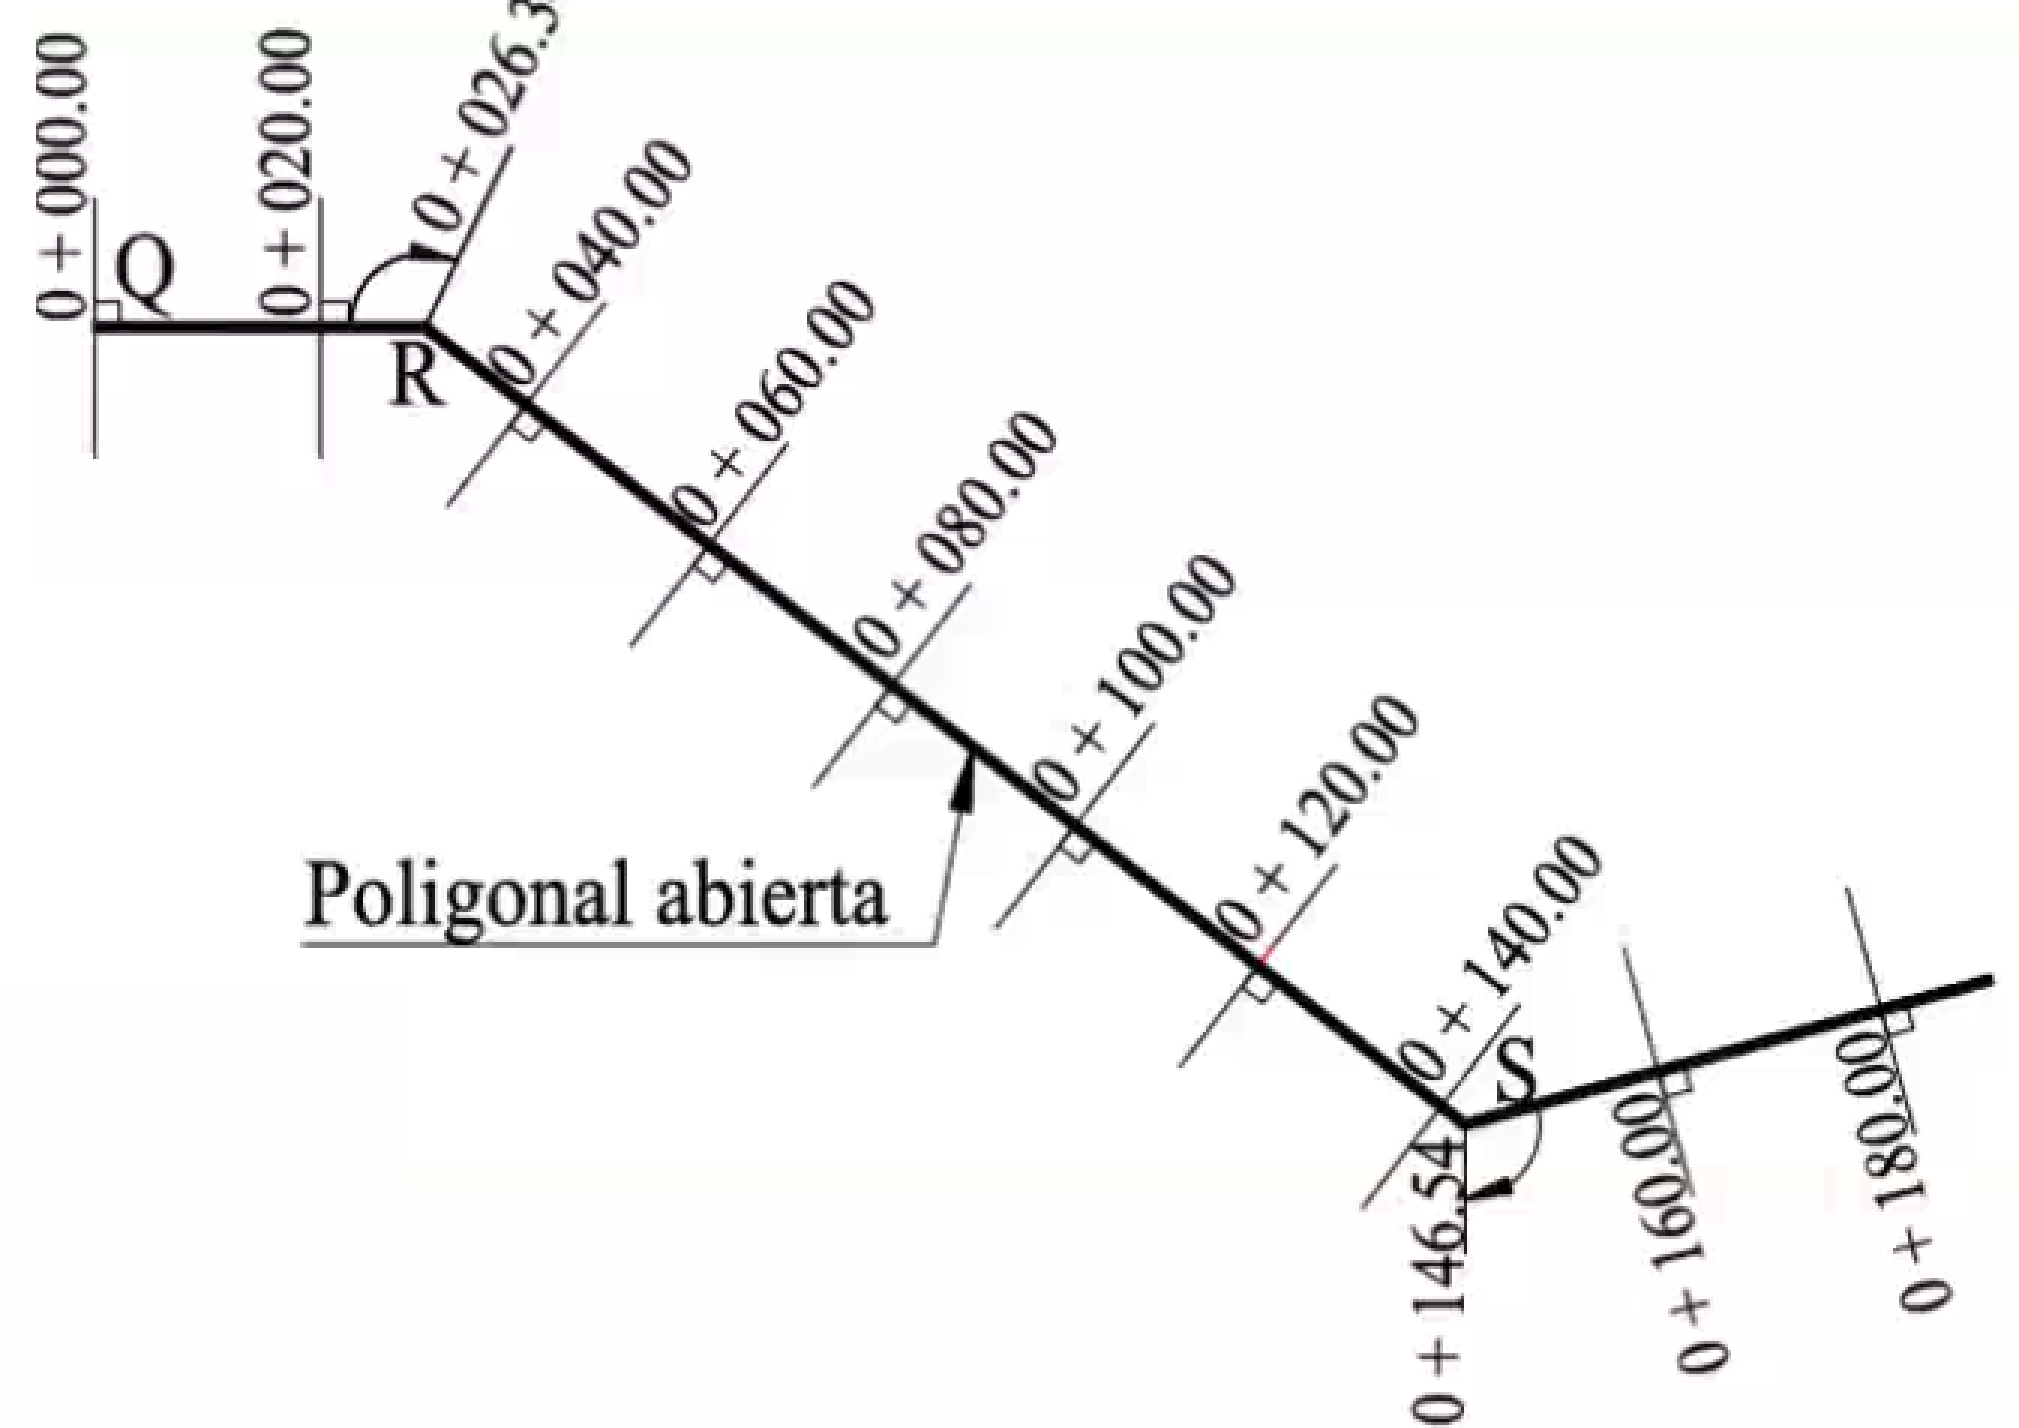
\includegraphics[width=0.5\textwidth]{ta28.png}}
  \caption{Método de secciones transversales}
  \label{ta28}
\end{figure}

Los puntos a levantar sobre cada sección se pueden establecer a separaciones regulares o equidistantes, pudiendo registrarse como cadenamientos si se miden como distancias acumuladas desde la LCA de la poligonal, o bien anotando las distancias parciales entre cada par de puntos consecutivos
Otra forma de ubicar los puntos es haciéndolo donde haya cambios de pendiente del terreno en la dirección del trazo, registrando, en tal caso también, distancias parciales o acumuladas.
Cualquiera que sea la forma como se midan las distancias, el trazo se prolonga hasta donde el proyecto lo quiera.

Una vez concluido el trazo de un lado de la sección, se da vuelta de campana al telescopio del instrumento para hacer el trazo de la parte opuesta y complementaria de la sección. Procediendo de manera totalmente análoga, para diferenciar la denominación de los puntos de uno y otro lado de la sección, sobre todo cuando las distancias son uniformes, se recomienda identificarlas, según sea el margen, derecha (D) o izquierda (I) en la que se ubiquen a partir de la línea de apoyo.

Se presenta a continuación, un cuadro de registro cuando se levantan puntos clave del terreno: 

\begin{table}[h!]
    \centering\begin{tabular}{cccccccccc}
    \multicolumn{4}{c}{Margen izquierda}                                                                                                                                                                                               & Sección                                                               & \multicolumn{5}{c}{Margen derecha}                                                                                                                                                                                                                                                             \\
    \begin{tabular}[c]{@{}c@{}}7.214\\ -2.568\end{tabular}  & \begin{tabular}[c]{@{}c@{}}9.105\\ -2.901\end{tabular} & \begin{tabular}[c]{@{}c@{}}8.806\\ -1.550\end{tabular} & \begin{tabular}[c]{@{}c@{}}7.152\\ -0.820\end{tabular} & \begin{tabular}[c]{@{}c@{}}1+540\\ Z=88.150m\\ LP=1.528m\end{tabular} & \begin{tabular}[c]{@{}c@{}}8.107\\ -3.652\end{tabular} & \begin{tabular}[c]{@{}c@{}}9.153\\ -3.028\end{tabular} & \begin{tabular}[c]{@{}c@{}}11.008\\ -2.207\end{tabular} & \begin{tabular}[c]{@{}c@{}}9.509\\ -0.803\end{tabular} & \begin{tabular}[c]{@{}c@{}}6.419\\ -0.759\end{tabular}    \\
                                                            &                                                        &                                                        &                                                        &                                                                       &                                                        &                                                        &                                                         &                                                        &                                                           \\
    \begin{tabular}[c]{@{}c@{}}10.418\\ -3.528\end{tabular} & \begin{tabular}[c]{@{}c@{}}5.259\\ -2.583\end{tabular} & \begin{tabular}[c]{@{}c@{}}6.827\\ -1.937\end{tabular} & \begin{tabular}[c]{@{}c@{}}9.297\\ -1.429\end{tabular} & \begin{tabular}[c]{@{}c@{}}1+560\\ Z=88.375m\\ LP=1.357\end{tabular}  & \begin{tabular}[c]{@{}c@{}}5.872\\ -2.120\end{tabular} & \begin{tabular}[c]{@{}c@{}}7.293\\ -3.058\end{tabular} & \begin{tabular}[c]{@{}c@{}}10.109\\ -3.528\end{tabular} & \begin{tabular}[c]{@{}c@{}}6.987\\ -2.981\end{tabular} & \begin{tabular}[c]{@{}c@{}}8.428\\ -2.785259\end{tabular} \\
                                                            &                                                        &                                                        &                                                        &                                                                       &                                                        &                                                        &                                                         &                                                        &                                                          
    \end{tabular}
    \caption{Ejemplo de un cuadro de registro para secciones transversales, cuando se levantan puntos clave del terreno}
    \label{tabta9}
\end{table}

Si se requiere conocer la ubicación de puntos de detalle o cualesquiera otros fuera de las secciones, se tendrá que emplear adicionalmente el método de radiaciones.

\begin{figure}[h!]
\centering
  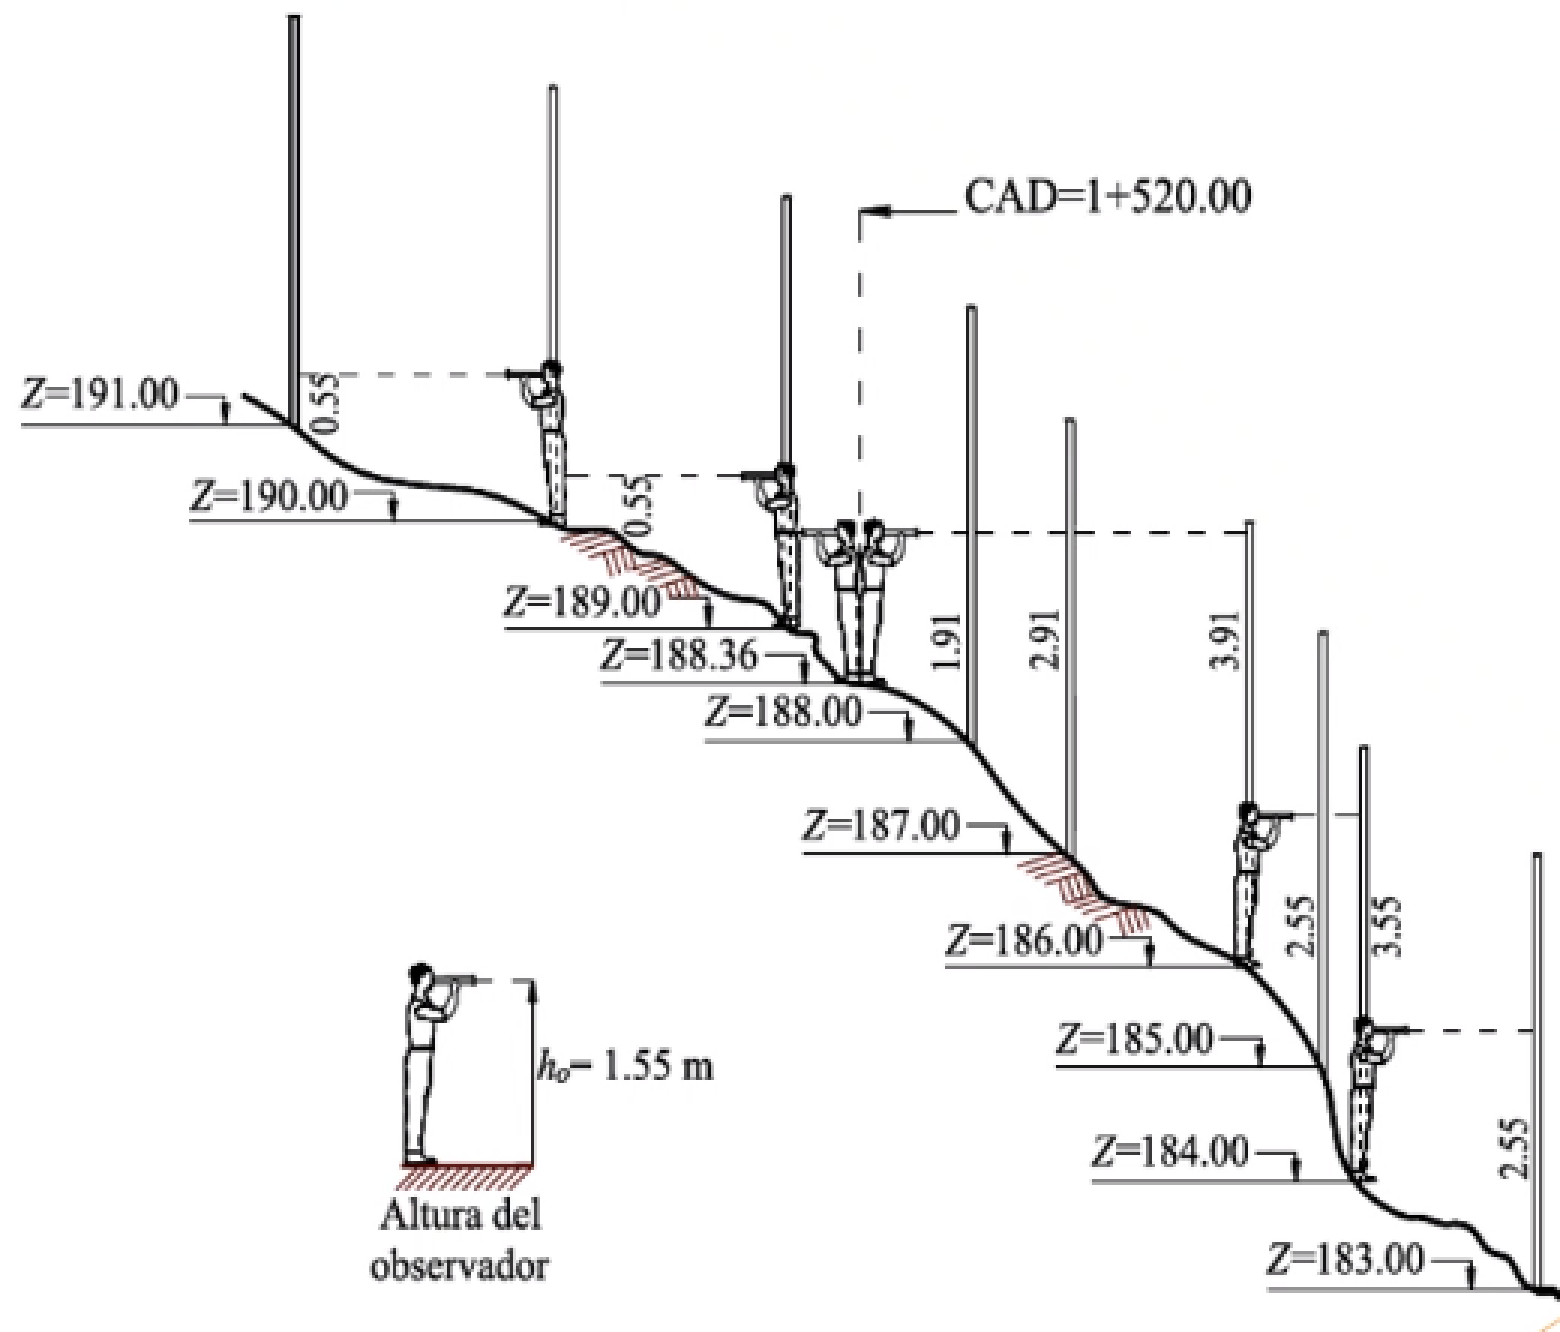
\includegraphics[width=0.5\textwidth]{ta29.png}
  \caption{Capturando puntos de cota cerrada con el nivel de mano}
  \label{ta29}
\end{figure}

La coordenada Z se obtiene haciendo los cálculos del cuadro correspondiente a la nivelación y su valor anota sobre el punto dibujado. Una vez que todos los puntos han sido ubicados en el plano con su respectiva coordenada Z, se puede proceder a dibujar curvas de nivel o los perfiles del terreno en cada sección, lo cual es perfectamente posible, pues se conocen las distancias entre los puntos y sus cotas, mismo que se grafican en el eje horizontal y vertical, respectivamente, de un sistema coordenado rectangular.

\subsubsection{Método de Cuadrícula}

El método de cuadrícula se considera el más preciso, por utilizar ordinariamente tránsito o teodolito y cinta para la ubicación de los puntos en el terreno y nivel montando para la obtención de sus elevaciones por el método de nivelación de perfil.

Se ha usado tradicionalmente en el levantamiento en el levantamiento de lotes agrícolas en donde se pretenda hacer el trazo de riego parcelario o bien proyectar y efectuar una nivelación de tierras, ya que en estos casos se requiere conocer, tanto la ubicación en planta como la elevación de los puntos, de manera muy precisa.

El método consiste en obtener la ubicación de los puntos para configuración mediante el trazo de un sistema de coordenadas rectangulares generando cuadros.

A la longitud de los lados de los cuadros se le denomina módulos de la cuadrícula y se denota por la letra M, y regularmente se recomienda igual a 20m para terrenos más o menos planos y de 25 o 30 m para terrenos con una condición intermedia de topografía 

\begin{enumerate}
    \item Se elige una esquina del terreno con un ángulo lo más próximos a $90^{\circ}$; en ella se define un punto que será el origen del sistema coordenado rectangular, y se le asignan las coordenadas (000,000) y en él se estaciona un instrumento para medir ángulos. En la dirección de ambos ejes rectangulares una magnitud igual de la mitad del módulo elegido; la cota de cada vértice del cuadro será representativa de un cuadro con longitud de lado igual a $M$
    \item El segundo paso consiste en colocar en el extremo opuesto del lado derecho del lote, una estaca, misma que se visa con el instrumento, constituyendo la línea resultante, el eje z del sistema coordenado, sobre la cual se miden distancias iguales al módulo de cuadrícula elegido, con cinta y se alínea con el instrumento para definir los puntos resultantes con estacas, sobre las que se anotan las coordenadas correspondientes a los puntos así definidos
    \item A partir de la dirección del eje x definido, se mide en el sentido antihorario, un ángulo de $90^{\circ}$ obteniendo en la dirección resultante el eje $y$ del sistema coordenado, sobre el cual se reporte el trazo descrito en el segundo punto
    \item Se pasa el teodolito al primer punto sobre el eje $x$ y se mide un ángulo de $90^{\circ}$ a partir de él, con lo que se obtiene una dirección paralela al eje $y$, sobre la cual nuevamente se repite el trazo, exactamente igual a lo explicado en el segundo punto. Véase la figura \ref{ta30} \begin{figure}[h!]
        \centering
          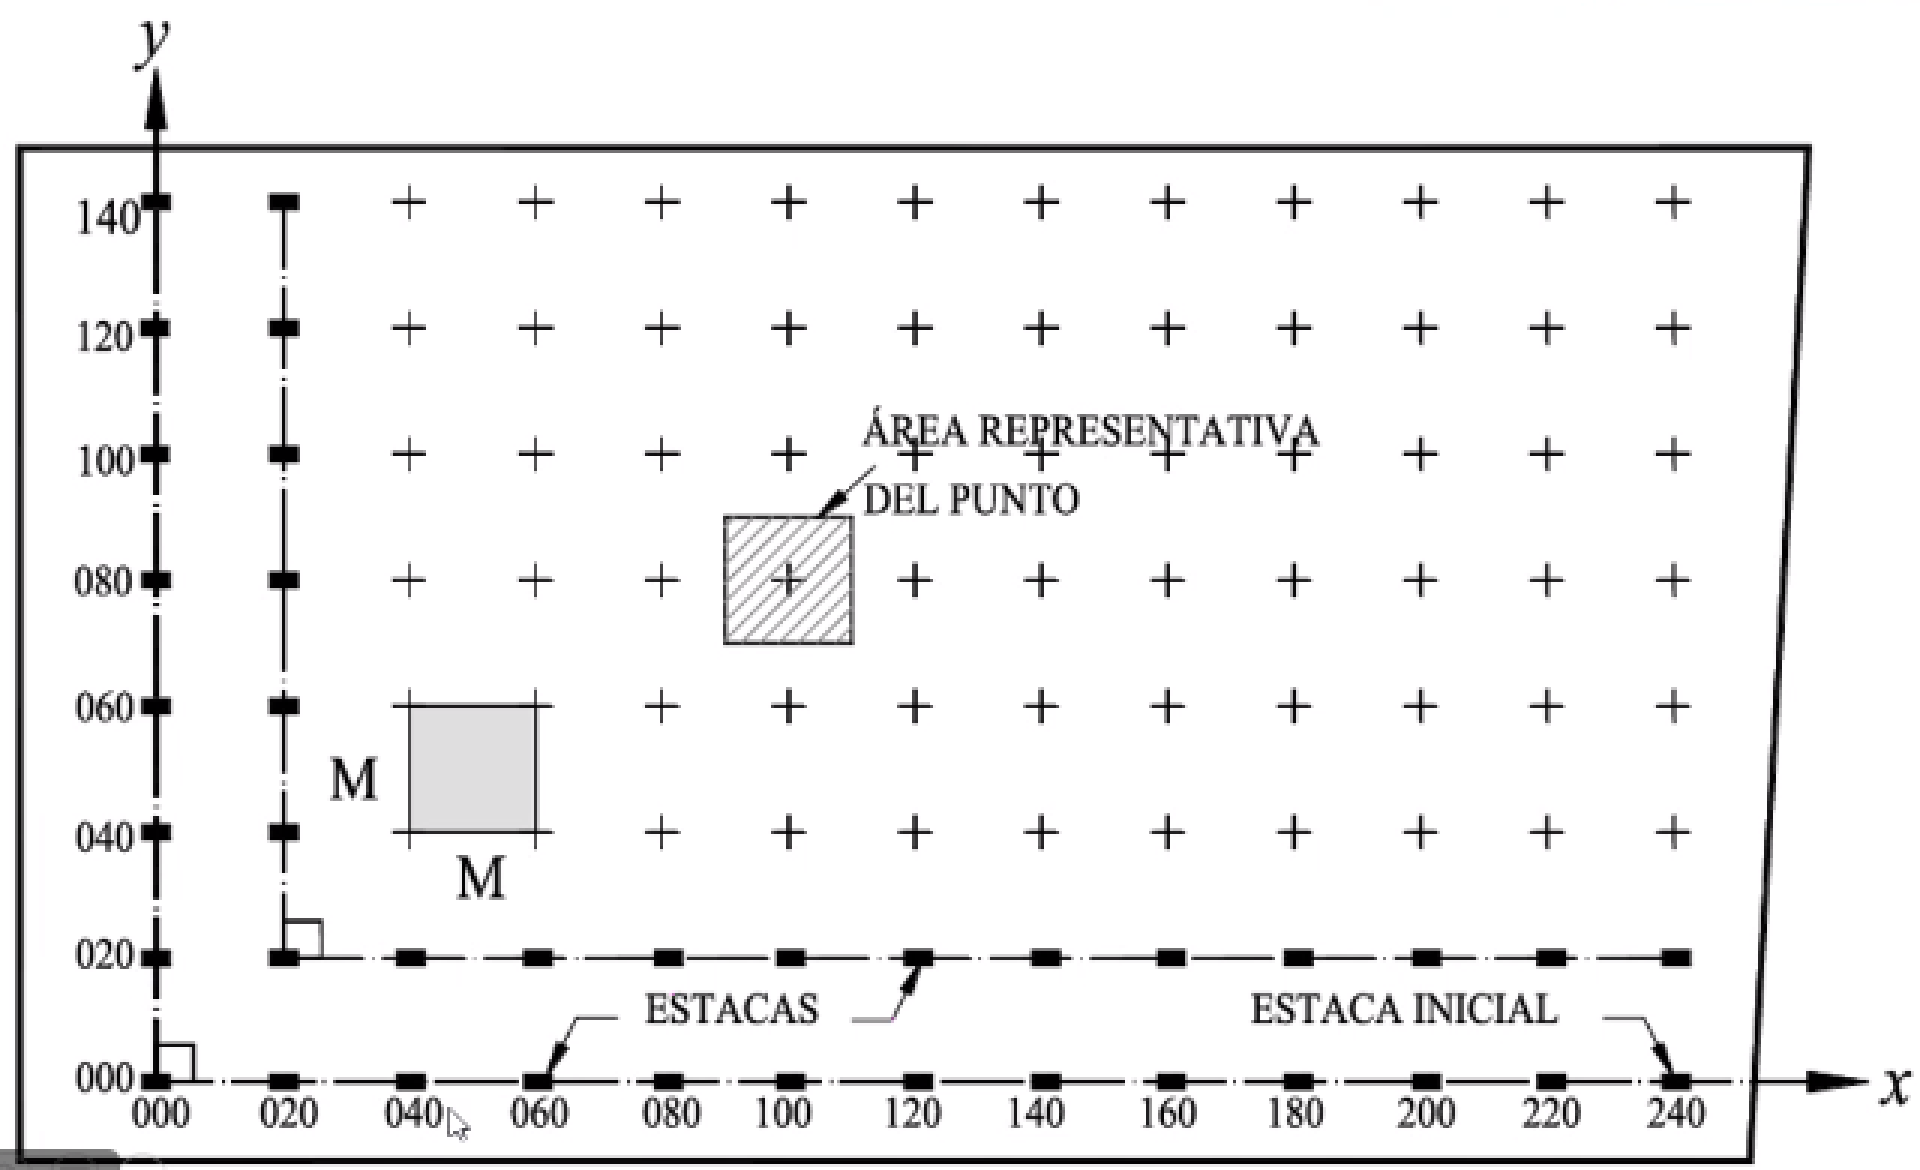
\includegraphics[width=0.5\textwidth]{ta30.png}
          \caption{Cuadrícula en el trabajo de campo}
          \label{ta30}
        \end{figure}
    \item El paso anterior se repite para trazar ahora una línea paralela al eje x a partir del primer punto sobre el eje y, con lo que se generan cuadros entre ambos pares de líneas y definidos físicamente por las estacas
    \item Los puntos restantes de la Cuadrícula, se ubican sobre el terreno, alineándose ``a ojo'' en ambas direcciones colocando balizas en los puntos correspondientes de ambos trazos en las direcciones $xy$
    \item Todo el proceso descrito en el punto anterior, se repite para ubicar los puntos restantes, colocando invariablemente en cada uno una estaca, sobre la cual se anotan sus coordenadas
    \item Estacionando el nivel en el sitio más conveniente, se procede a hacer la nivelación de todos los puntos por nivelación de perfil. Definiendo el punto (000,000) o cualquiera otro como banco de nivel.
    \begin{figure}[h!]
        \centering
          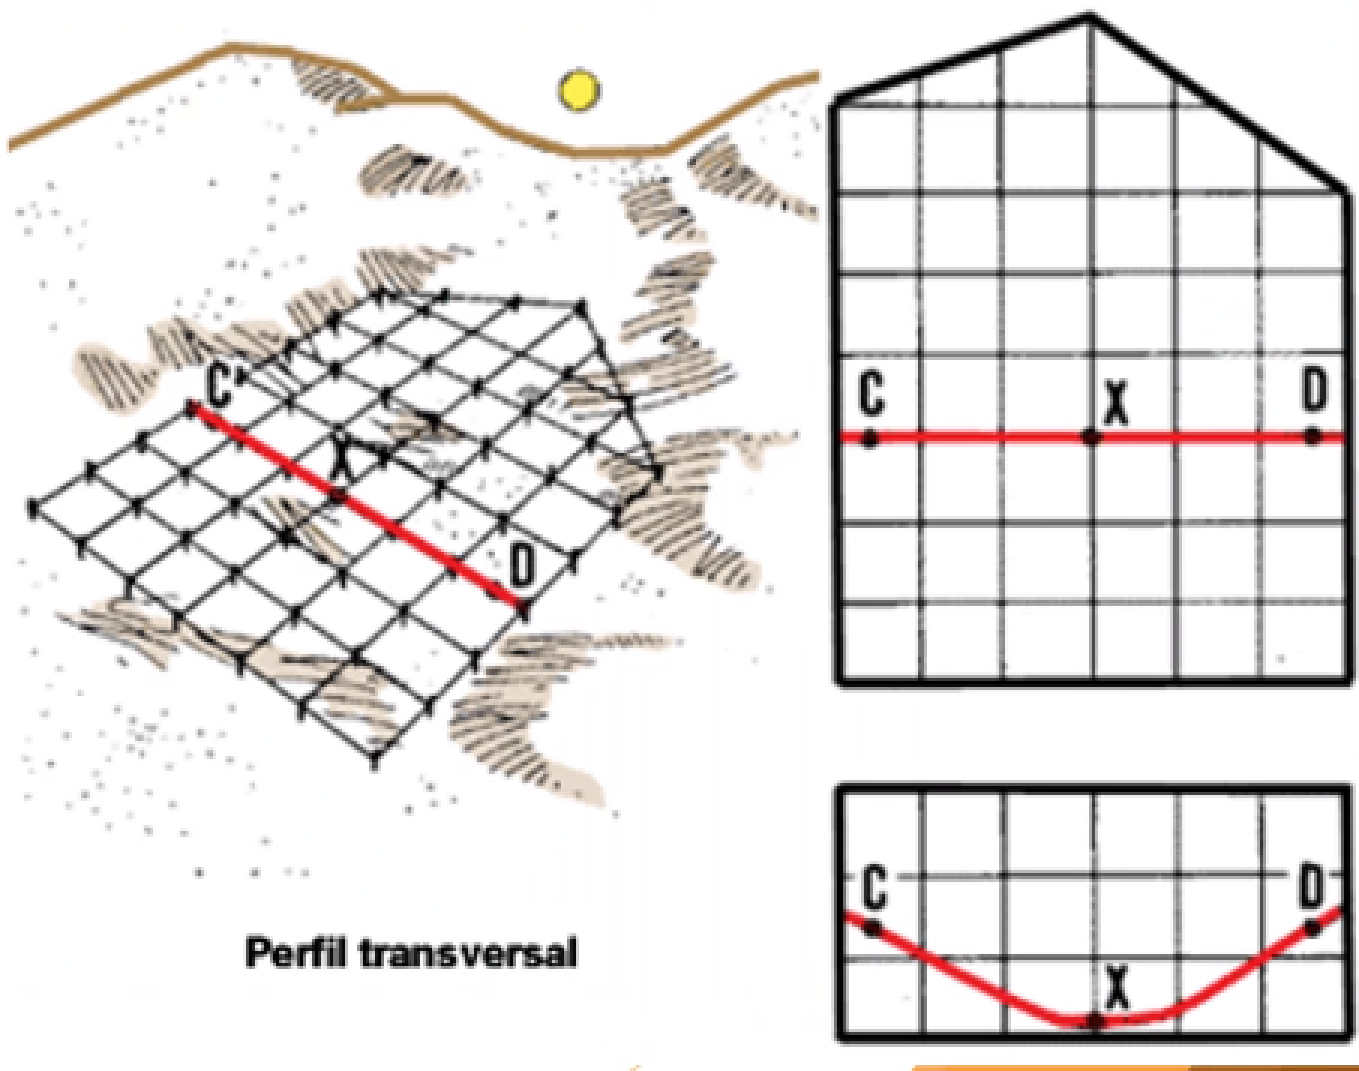
\includegraphics[width=0.5\textwidth]{ta31.png}
          \caption{Nivelación de perfil}
          \label{ta31}
        \end{figure}
\end{enumerate}

\section{Instrumentos y sistemas topográficos}

\begin{definition}[Instrumentos topográficos]
    A los dispositivos de medición que son un sólo cuerpo o unidad y en el que se localiza la parte o componente principal de medición tal como la graduación, la aguja imantada, la aliada, los círculos graduados (Ya sean mecánicos, óptico o eléctricos) o los sensores o cámaras, sin considerar ningún aditamento, tal como la cinta, la brújula, el trípode, nivel de mano, baliza, prisma, estadal, plomada de cordón, etc.
\end{definition}

\begin{definition}[Aditamentos]
    Son los elementos adicionales al instrumento topográfico, que se requiere para su instalación o para efectuar la medición para la que se utiliza.
\end{definition}

\begin{table}[h!]
    \centering\begin{tabular}{@{}cccccc@{}}
    \toprule
    \multirow{2}{*}{\begin{tabular}[c]{@{}c@{}}Tipo de medición\\ o proceso\end{tabular}} & \multicolumn{3}{c}{Tradicionales}                                                                                                                                                                           & \multicolumn{2}{c}{Electrónicos}                                                                                                                      \\ \cmidrule(l){2-6} 
                                                                                          & \begin{tabular}[c]{@{}c@{}}1ra \\ generación\end{tabular}             & \begin{tabular}[c]{@{}c@{}}2da\\ generación\end{tabular}        & \begin{tabular}[c]{@{}c@{}}3ra\\ generación\end{tabular}          & Modernos                                                                    & Actuales                                                                \\ \cmidrule(r){1-1}
    Distancias                                                                            & Cinta                                                                 & Odómetro                                                        & Estadia                                                           & Distanciómetro                                                              &                                                                         \\
    Desniveles                                                                            & Nivel de mano                                                         & Clisímetro                                                      & Nivel tradicional                                                 & \begin{tabular}[c]{@{}c@{}}Nivel automático,\\ láser y digital\end{tabular} &                                                                         \\
    Ángulos                                                                               & Brújula                                                               & \begin{tabular}[c]{@{}c@{}}Tránsito y \\ planchera\end{tabular} & Teodolito óptico                                                  & \begin{tabular}[c]{@{}c@{}}Teodolito \\ Electrónico\end{tabular}            & Estación total                                                          \\
    Cálculo                                                                               & Ábaco                                                                 & \begin{tabular}[c]{@{}c@{}}Regla de \\ Cálculo\end{tabular}     & Calculadora                                                       & Computadora                                                                 &                                                                         \\
    Orientación                                                                           & Astrolabio                                                            & Brújula                                                         & \begin{tabular}[c]{@{}c@{}}Orientación\\ astronómica\end{tabular} & Brújula electrónica                                                         & \begin{tabular}[c]{@{}c@{}}Sensores remo-\\ tos y sistemas\end{tabular} \\
    \begin{tabular}[c]{@{}c@{}}Posicionamiento\\ Geográfico\end{tabular}                  & \begin{tabular}[c]{@{}c@{}}Observación a\\ las estrellas\end{tabular} &                                                                 & Orientación astronómica                                           & GPS                                                                         & \begin{tabular}[c]{@{}c@{}}De información\\ geográfica\end{tabular}     \\ \bottomrule
    \end{tabular}
    \caption{Instrumentos, dispositivos, equipos para efectuarlas, son su herramienta principal y han ido evolucionando paralelamente al desarrollo de la ciencia y tecnología}
    \label{tabta10}
\end{table}

Los Instrumentos en conjunto con los aditamentos que utilizan para ponerlos en estación, soportarlo o transportarlos y como apoyo o complemento para realizar la medición:

\begin{itemize}
    \item Nivel topográfico, tripié y estadales o receptor de señal (para el caso de los láser)
    \item Tránsito o teodolito, tripié, estadales, balizas y plomada
    \item Distanciómetro (y teodolito si se instala sobre él), tripié, bastón y prisma; y brújula
    \item Estación total, tripié, bastón y prisma y brújula
    \item Los instrumentos receptores de señal de posicionamiento global o antenas (que de ordinario se requieren dos), radios, las señales de satélite, las señales de la red geodésica nacional
    \item El sensor de imagen, de señal RADAR o de señal de LIDIAR, vehículo aéreo no tripulado (VANT o drone), dispositivo de control de vuelo
\end{itemize}

Una cinta o una brújula son instrumentos topográficos por sí mismos, en tanto que se emplean directa e independientemente para hacer mediciones específicas.

\begin{definition}[Sistemas topográficos]
    Cuando a los equipos topográficos, se les adiciona las tecnologías, ya sean como complementos que se requieren para efectuar la medición o para el procesamiento de los datos hasta que se obtienen los resultados finales, que en general serán las coordenadas de los puntos que se emplearán para la elaboración de los planos, así como las que se requieren para su elaboración
\end{definition}

\begin{definition}[Instrumentos tradicionales]
    Son aquellos que en su construcción sólo se conformaron de partes físicas y mecánicas y para su funcionamiento se constituyen de medio ópticos
\end{definition}

Los instrumentos que están constituidos por sistemas automatizados y/o por componentes electrónicos y muestran sus valores medidos en forma digital son \textbf{Instrumentos electrónicos} ó modernos. 

Existen dos tipos de lectura óptica: los repetidores y los direccionales;

Igual que los tránsitos tienen la función de medir ángulos.

Difieren de los tránsitos en apariencia, pues son generalmente más compactos, ligeros y aerodinámicos y tienen círculos de vidrio finamente graduados que se visualizan con un
microscopio.

Otras características constructivas: 

\begin{enumerate}
    \item Los telescopios son cortos, retículas grabadas en vidrio, equipados con mirillas de rifle para puntería gruesa
    \item Círculo vertical indexado al zenit
    \item Los trípodes ajustables y bases de nivelación intercambiables con otros instrumentos o aditamentos
    \item Con plomada óptica
    \item Tres tornillos niveladores y nivel esférico
    \item No tienen brújula, como lo es en el tránsito.
\end{enumerate}

Características generales de los Instrumentos Modernos
\textbf{Desventajas:}
\begin{enumerate}
    \item Tienen altos costos que superan a los de los Instrumentos Tradicionales del orden de entre 5 y hasta 20 o más veces. 
    \item Su manejo requiere conocimientos especiales o particulares y, por lo tanto, es necesaria una capacitación específica, no sólo para cada tipo de instrumento sino para cada modelo.
    \item Dados sus componentes electrónicos, generan campos electromagnéticos que limitan su uso en áreas cercanas a redes eléctricas, por ejemplo. dy Su revisión, servicio y mantenimiento debe ser frecuente, realizado por personal especializado y en laboratorios o talleres especiales.
\end{enumerate}

Características generales de los Instrumentos Modernos

Puesta en Estación de teodolitos, ET, Receptores GPS

\begin{enumerate}
    \item Se emplaza el tripode sobre el PCA, procurando lo más posible que se cumplan las tres condiciones indicadas en el primer párrafo, es decir que la plomada quede centrada en el PCA, la base del tripode esté nivelada y a una altura tal que el telescopio quede a la altura del ojo del observador
    \item Se coloca la base nivelante sobre el tripode y se acopla mediante el tornillo de sujeción que trae provisto en el centro de su cabeza el tripode cuidando que quede lo más centrado posible
    \item Colocando entre dos patas del tripode, dejando el de enfrente y procurando que la base nivelante permanezca aproximadamente horizontal y a la altura deseada, se centr plomada en la marca del PCA
    \item Aflojando y apretando los tornillos que sujetan las extensiones de las patas, se alargan o acortan éstas según se requiera, con los que se sube o baja la base del lado correspondiente, a fin de centrar la burbuja del nivel esférico; para esta operación se debe tener presente que la burbuja siempre se ubica en la parte más alta de su área de movimiento, con lo que se determina si la pata correspondiente del tripode debe alargarse o acortarse, para elevar o bajar la base nivelante en el lado correspondiente.
    \item Se debe verificar que la plomada siga posicionada en el punto y centrar nuevamente, moviendo según se requiera los tornillos niveladores
    \item Repetir los pasos 4 y $5^{\circ}$ cuantas veces sea necesario hasta que el movimiento de la plomada (estando centrada la burbuja), para su centrado sea mínimo, que se pueda hacer desplazando la base nivelante aflojando el tornillo
\end{enumerate}

\subsubsection{Teodolitos electrónicos}

Pueden leer y desplegar automática y simultáneamente ángulos horizontales y verticales en una pantalla LCD
\begin{itemize}
    \item Los ángulos horizontales pueden medirse en sentido horario y antihorario
    \item Los ángulos verticales pueden ser cenitales  o alturas
    \item El cero de ambos círculos se pueden fijar en cualquier valor
    \item Pueden ser repetidores
    \item Su precisión puede ser de hasta un segundo
\end{itemize}
El operador debe realizar la puesta en estación del instrumento, apuntar el telescopio a los puntos de medición, definir el formato de medición, e indicarle al aparato que la efectúe

En todos los casos, para la interacción del operador con el aparato, tienen dos tornillos, uno para el movimiento horizontal y otro para el vertical y un botón de enfoque del objetivo.

Algunos están provistos de memoria electrónica para el almacenamiento de las lecturas.

\begin{table}[h!]
    \centering
    \begin{tabular}{@{}ll@{}}
    \toprule
    Característica                                                   & Valor y unidad     \\ \midrule
    Precisión                                                        & $2^{\prime\prime}$ \\
    Resolución                                                       & $1^{\prime\prime}$ \\
    \begin{tabular}[c]{@{}l@{}}Aumento del\\ telescopio\end{tabular} & 30x                \\
    Imagen                                                           & Directa            \\
    Enfoque mínimo                                                   & 0.90m              \\
    Pantalla LCD                                                     & Dos                \\
    Puerto de salida                                                 & N/A                \\
    \begin{tabular}[c]{@{}l@{}}Compensador \\ vertical\end{tabular}  & S+i                \\
    Puntero láser                                                    & No                 \\ \bottomrule
    \end{tabular}
    \caption{Características técnicas recomendadas para teodolitos electrónicos}
    \label{tabta11}
\end{table}

Los medidores electrónicos de distancias (MED) son instrumentos que determinan las longitudes indirectamente a través de la medición del tiempo que tarda la energía electromagnética en viajar con velocidad conocida (la de la luz) de ida y regreso de un extremo a otro de línea.
\begin{equation}
    v = \frac{D}{t}\implies D = v\cdot t
\end{equation}

Los instrumentos MED, hacen mediciones precisas y rápidas;

Miden magnitudes pequeñas o grandes sobre cuerpos de agua, autopistas con gran tráfico, o terrenos que son inaccesibles para mediciones con cinta;

No importa las irregularidades u obstáculos del terreno; basta con que los puntos que definen la línea a medir sean intervisibles.

El instrumento MED se coloca sobre un teodolito con el que se lanza la visual, por lo que la altura del reflector ($hr$) debe ser igual a la de instrumento $(hi)$

Existen dos tipos de aparatos y sistemas:

\begin{enumerate}
    \item \textbf{Electro-ópticos:} Emiten señales electromagnéticas (luz láser o infrarrojo), requieren un equipo emisor receptor y un reflector. Las mediciones se afectan por temperatura y presión atmosférica
    \item \textbf{Microondas:} Emiten señales de radio, requieren un equipo emisor receptor en ambos puntos y se afectan por temperatura, presión atmosférica y humedad relativa, véase la figura \ref{hb32}
\end{enumerate}
\begin{figure}[h!]
\centering
  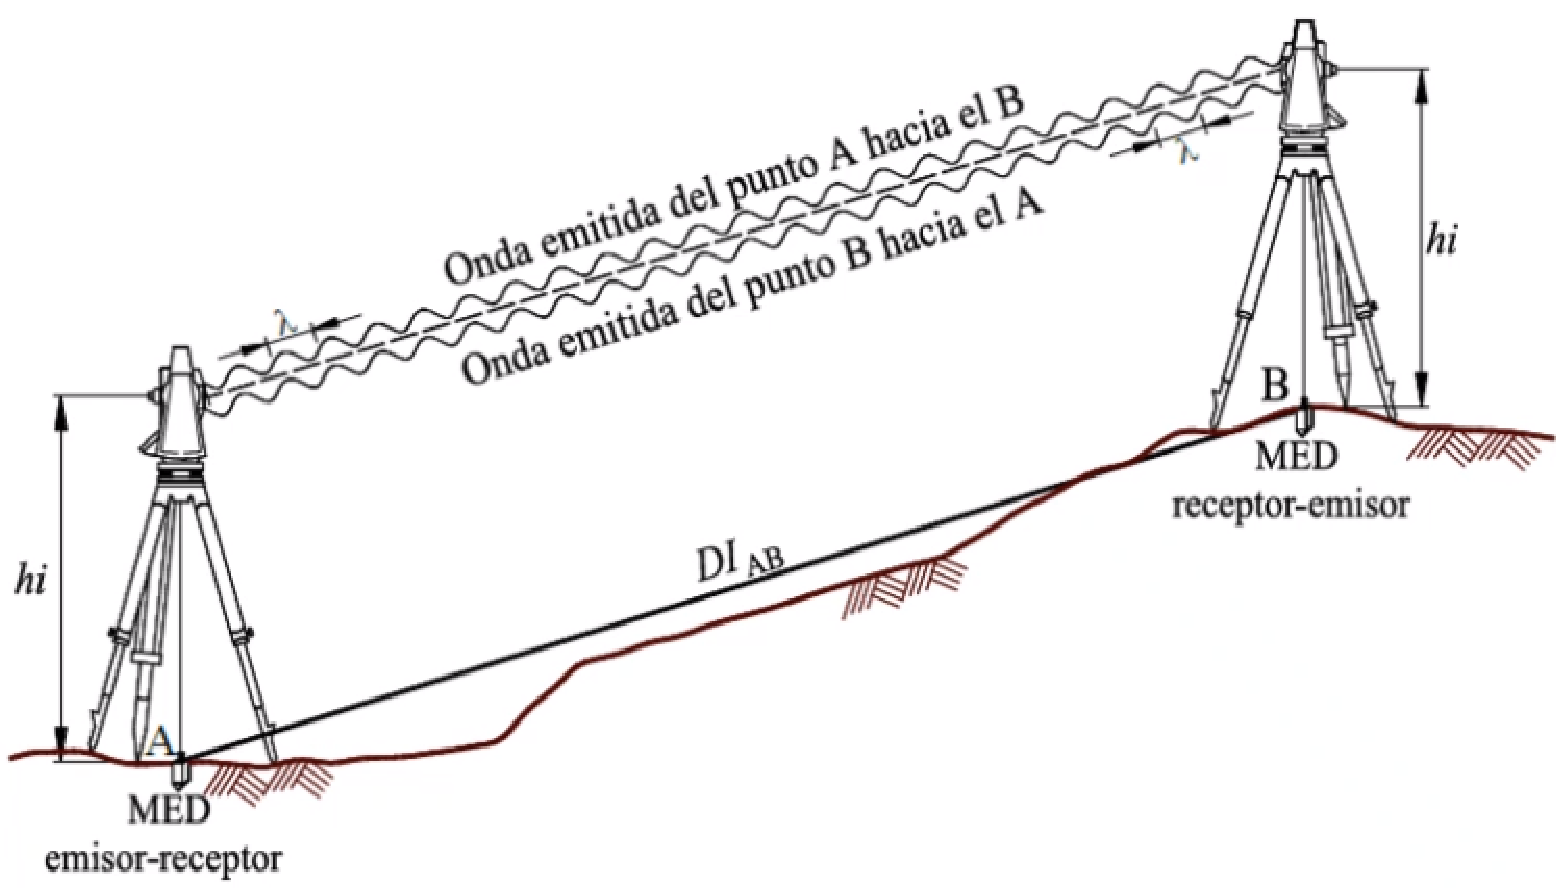
\includegraphics[width=0.5\textwidth]{ta32.pdf}
  \caption{Principios de medición de microondas}
  \label{hb32}
\end{figure}
Los principios de medición de los MED electro-ópticos, están dadas por la velocidad de la luz:
\begin{equation}
    V = \frac{c}{r}
\end{equation}
donde $r=1.003$: refracción de la atmósfera
y también la energía electromagnética:
\begin{equation}
    v = f\lambda
\end{equation}
De aquí podemos derivar las siguientes ecuaciones de la figura \ref{ta33}
\begin{align}
    DI = n\frac{\lambda}{2}\\
    DI =\frac{n\lambda + p}{2}\\
    p =\frac{s\lambda}{360}\\
    DI =\left(\frac{n}{2} + \frac{a}{720}\right)\lambda
\end{align}
Para $n=4$ y $p=0.602\lambda$, entonces:
\begin{equation*}
    DI =\left(\frac{4}{2} + \frac{216.7}{720}\right)_0 = 46.020
\end{equation*}

\begin{figure}[h!]
\centering
  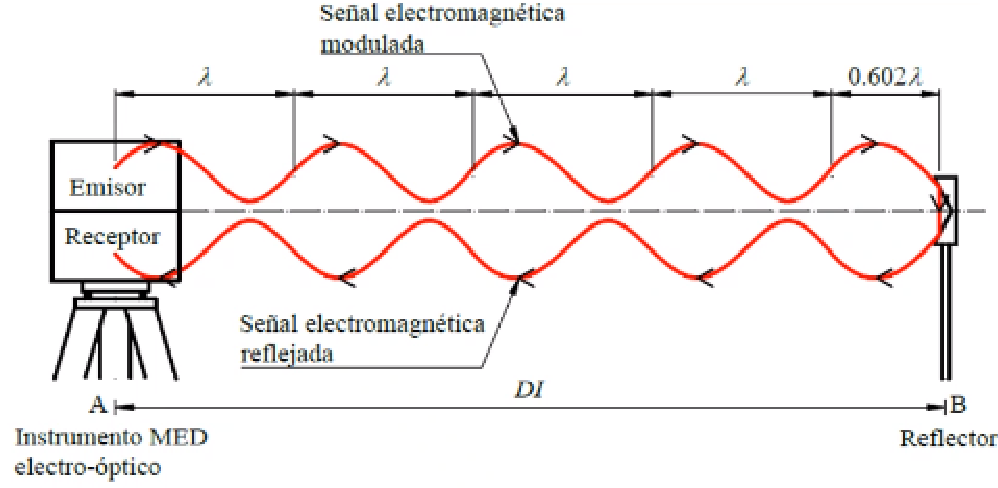
\includegraphics[width=0.5\textwidth]{ta33.pdf}
  \caption{Distanciómetros (MED)}
  \label{ta33}
\end{figure}

Para el cálculo de reducción de la $DI$ a $DH$ si $hi=hr$
\begin{align}
    DH = \sqrt{DM^2 - DE^2}\\
    DH = DM -\frac{DE^2}{2DM}\\
    DE =\left(Z_A + hi\right) -\left(Z_B + hr\right)\\
    \Delta AZ = \frac{(hi - hr)\sin{(AZ_v)}}{DM\times 206.265}
\end{align}

\begin{figure}[h!]
\centering
  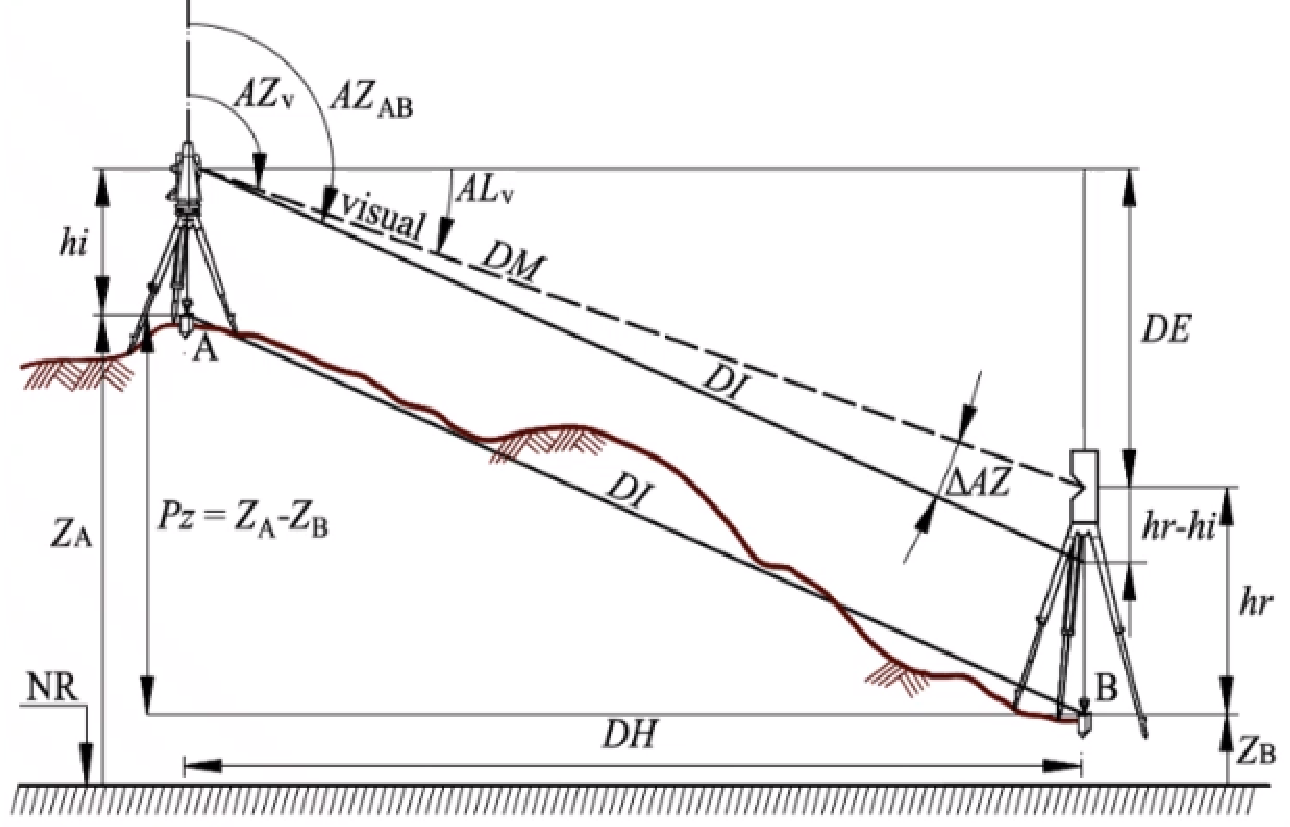
\includegraphics[width=0.5\textwidth]{ta34.pdf}
  \caption{Procedimiento para la medición de los MED}
  \label{ta34}
\end{figure}

Es fundamental considerar los errores en estas mediciones, pudiendo clasificar lo siguiente
\begin{itemize}
    \item Errores personales \begin{itemize}
        \item Imprecisión en la instalación del instrumento y del reflector
        \item Falsas mediciones de altura del instrumento y del reflector
        \item Determinación errónea de la $Pa$ $T$ y $M_R$
    \end{itemize}
    Pueden minimizarse operando con cuidado y usando barómetros, termómetros y psicrómetros de gran calidad
    \item Errores instrumentales \begin{itemize}
        \item Por desajuste
        \item Por emisión de frecuencias erróneas (falsas $\lambda$)
        \item Error del prisma ``constante de prisma''
    \end{itemize}
\end{itemize}

\subsubsection{Estación total}

La ET combinan e integran en una sola unidad, tres componentes básicos, a saber: un Instrumento Medidor Electrónico de Distancias para la medición de la Distancia Inclinada DI, un teodolito electrónico digital para hacer la visualización de los puntos y medir los ángulos (uno horizontal y uno vertical) de la visual y una computadora o microprocesador para hacer los cálculos necesarios para obtener las proyecciones de la distancia inclinada medida y determinar las coordenadas XYZ de los puntos observados y desplegarlos y almacenados electrónicamente.


\subsubsection{Características constructivas y operativas}
Las características de todos los instrumentos topográficos modernos, tales como:
\begin{itemize}
    \item Tres tornillos niveladores
    \item Niveles de burbuja central y electrónicos
    \item Plomada óptica para los movimientos
    \item Computadora
    \item Mira de rifle
    \item Lectura e introducción digital de datos
    \item Alta precisión
    \item Alto rendimiento
\end{itemize}

\subsection{Estación total}

Existen ciertas especificaciones técnicas

La precisión lineal o error estándar lineal, dado en partes por millón (ppm) y que equivale a error accidental que se puede cometer al hacer una medición por cada $km$ medido
La precisión angular o error estándar angular, que es la aproximación con la que miden los ángulos horizontales y verticales
El alcance del instrumento en las mediciones lineales con un prisma o con los que vaya a disponer en un caso dado,
La amplificación de la imagen al visualizarla por el telescopio y la duración de la carga de las baterías.

\subsubsection{Configuración al ponerse en estación}

El instrumento debe orientar, visando un punto de control y apoyo (PCA), de cuya línea de control y apoyo (LCA) se debe conocer sy azimut previamente definido, ya sea por medición a partir de las LCA anteriores, o con una brújula, si se trata de la primera $LCA$ del trabajo.
Se introduce el nombre del punto estación y sus coordenadas $X_E,Y_E,Z_E$
Se introduce la altura del instrumento $hi$ y la altura de reflector $hr$, este dato normalmente puede cambiarse cada que sea necesario.
Se define el nombre del trabajo, que en general corresponde con el nombre del archivo donde se almacenarán los datos y los resultados del levantamiento,
Se define la denominación del primer punto de los que se van a levantar.

\subsubsection{Configuración al ponerse en estación}

Las unidades para las mediciones lineales y angulares. El sentido de medición de los ángulos horizontales (horario o antihorario).
El origen de los ángulos verticales: el zenit (AZ) o el horizonte (AL)
Las resolución con la que se mostrarán los valores angulares en la pantalla.
Las variables a mostrar en la pantalla de las que mide o calcula ($DH,P_x,P_y,P_z,Az$ y $AZ$)
Los valores de la temperatura, la presión atmosférica para corregir las mediciones lineales.

Datos que se le deben proporcionar:
\begin{itemize}
    \item Nombre de la estación
    \item Coordenadas de la estación ($X_e,Y_e,Z_e$)
    \item Altura del instrumento ($hi$)
    \item Altura del reflector o prisma ($hr$ o $ap$)
    \item Orientar el instrumento
\end{itemize}
Valores que mide:
Distancia inclinada de la estación al $PV$ azimut ($az$) y distancia zenital ($AZ$) o altura ($AL$)

Los valores que calcula y proporciona:
\begin{itemize}
    \item Proyecciones de la visual ($P_x,P_y,P_z$)
    \item Distancia horizontal ($DH$)
    \item Coordenadas del PV ($X_pY_p,Z_p$)
\end{itemize}

\begin{figure}[h!]
\centering
  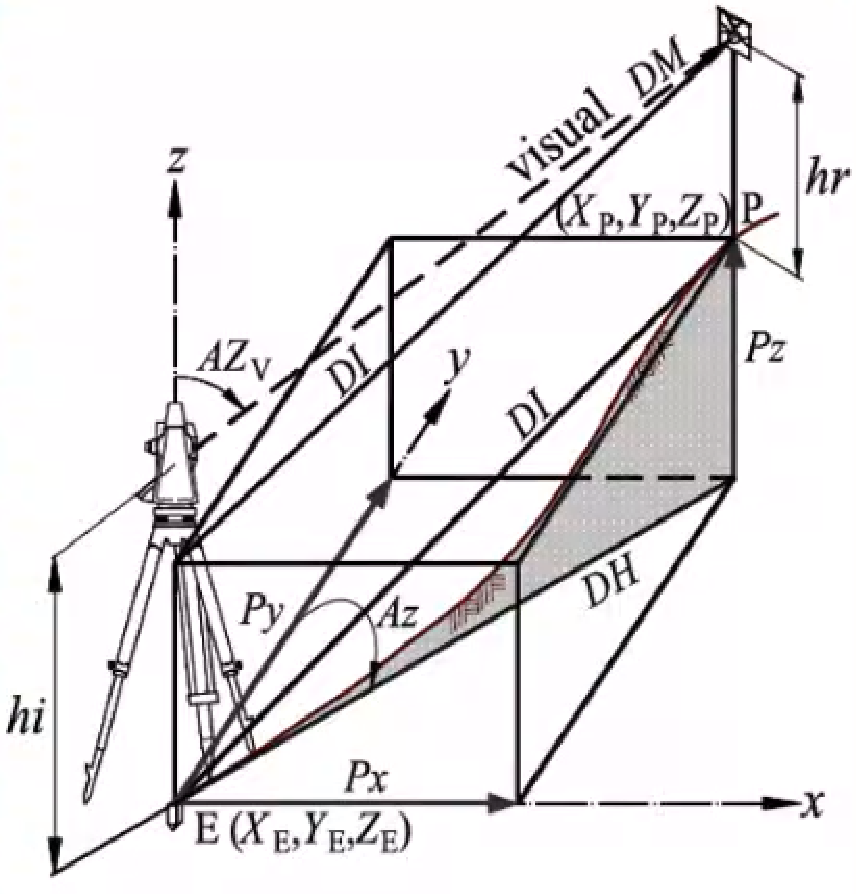
\includegraphics[width=0.5\textwidth]{ta35.pdf}
  \caption{Estación total, datos mediciones y resultados}
  \label{ta35}
\end{figure}

\subsubsection{Proceso de medición}

Se deben seguir una serie de pasos:
\begin{itemize}
    \item Se pone en estación y se configura el instrumento
    \item Se coloca el reflector en el punto a determinar sus coordenadas
    \item Se visa con el telescopio de la ET el centro de reflector y se oprime la tecla que da la orden de hacer la medición, efectuar los cálculos necesarios y almacenar en el archivo definido los datos y valores determinados, incluyendo las coordenadas del punto observado. COn lo que la ET: \begin{itemize}
        \item Mide la longitud de la visual (DM), el azimut de la visual ($Azv$) y el ángulo vertical definido para la visual
        \item Calcula la distancia horizontal $DH$, las proyecciones $P_x,P_y,P_z$ y las coordenadas del punto visado
        \item Guarda todos los valores introducidos, medidos y calculados y despliega los que se le indiquen durante la configuración.
    \end{itemize}
\end{itemize}


\begin{align}
    DH = DM \times \sin{(AZ_v)}\\
    Pz = DM \times \cos{(AZ_v)} -(hr - hi)\\
    DI = \sqrt{DH^2 + Pz^2}
\end{align}
\begin{figure}[h!]
\centering
  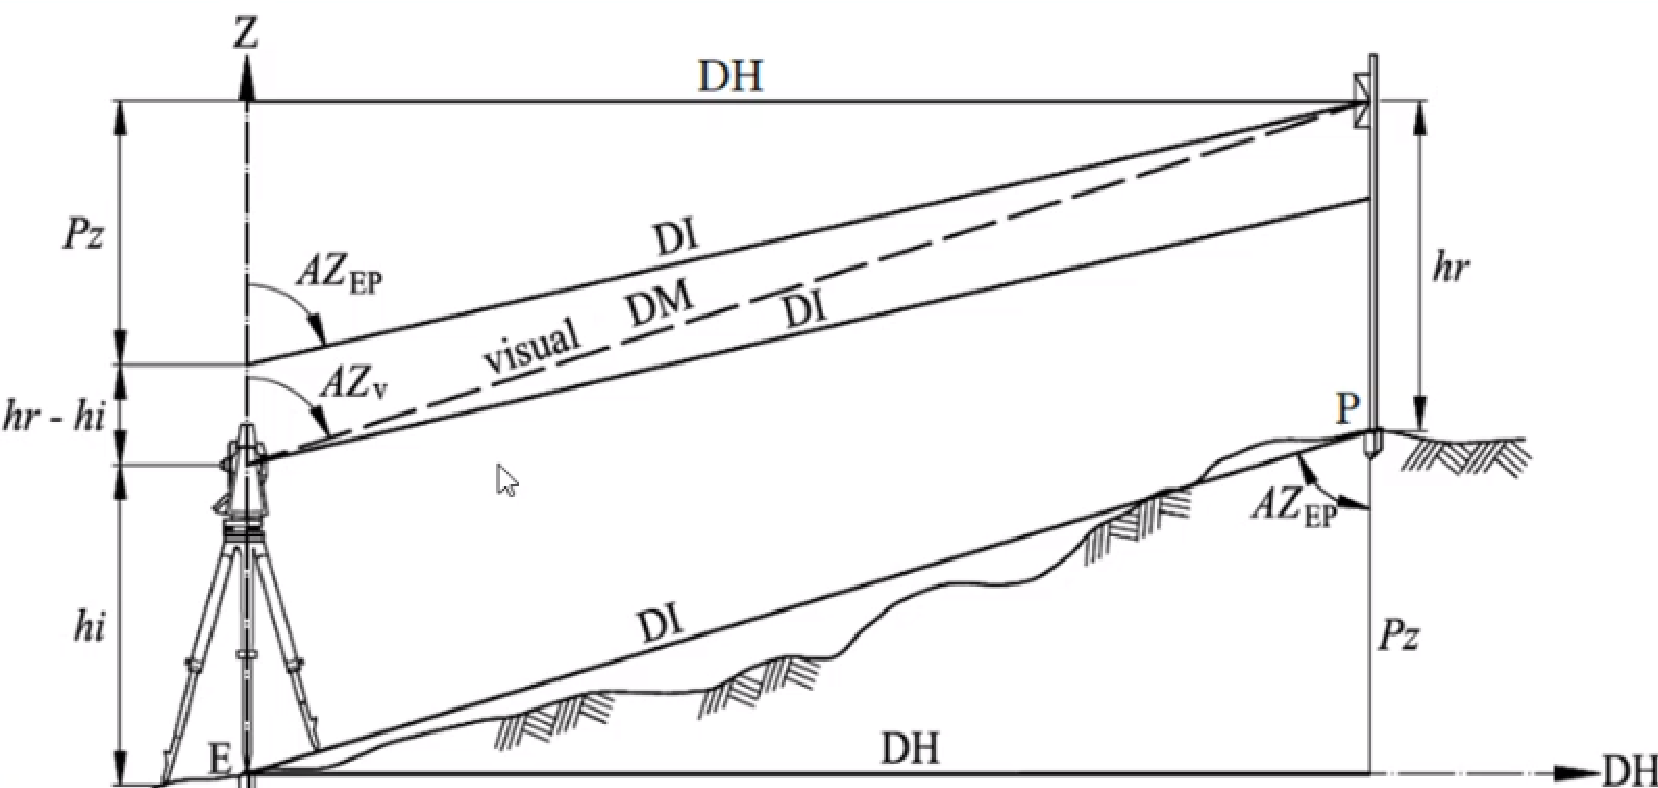
\includegraphics[width=0.5\textwidth]{ta36.pdf}
  \caption{Estación total}
  \label{ta36}
\end{figure}

Una ET se estaciona en el PCA G cuyas coordenadas son (5,578.562; 8,452.789; 1,785.923), a una altura de 1.615 m y se visa el punto G9, en el que se coloca el reflector a una altura de 2.854 m; calcular las coordenadas que el instrumento determinó para el punto 69 si los valores medidos fueron: $DM= 385.415 m, AzV= 275^{\circ} 54^{\prime} 09^{\prime\prime} y AZY= 086^{\circ} 17^{\prime} 36^{\prime\prime}$

\textit{ Sol. }
\begin{align*}
    &DH = 385.415 \times \sin{(086^{\circ} 17^{\prime} 36^{\prime\prime})} = 384.609m\\
    &Pz = 385.415 \times \cos{(086^{\circ} 17^{\prime} 36^{\prime\prime})} -(2.854 - 1.615) = 23.678mm\\
\end{align*}
\begin{align*}
    &P_x = 384.609 \times \sin{(275^{\circ} 54^{\prime} 09^{\prime\prime})} = - 382.570m\\
    &P_y = 384.609 \times \cos{(275^{\circ} 54^{\prime} 09^{\prime\prime})} = 39.552\\
\end{align*}
\begin{align*}
    &X_{G_9} = 5578.562 +( - 82.570) = 5195.992m\\
    &X_{G_9} = 8452.789 + 39.552 = 8492.341m\\
    &Z_{G_9} = 1785.923 + 23.678 =1809.601m
\end{align*}



\subsection{Sistema de PGS}

En 1978 el Departamento de Defensa de los EUA puso en marcha el Sistema de Posicionamiento Global (GPS) para el posicionamiento de puntos sobre la superficie terrestre a partir de sus coordenadas geográficas (Latitud, Longitud y Altitud) para fines militares.
Su componente espacial lo constituye la constelación NAVSTAR (NAVigation System Time And Range: Sistema de Navegación de Tiempo y Distancia), que proporciona la ubicación de un conjunto de satélites en espacio y tiempo.

En 1967, EUA disponía de un sistema de navegación vía satélite, utilizando el método Doppler, para su sistema de defensa y fue en el 2000 cuando autorizaron reducir el error de 100 a 10 m para uso civil.

\begin{itemize}
    \item Global positioning system-NAVegation satélite timming and ranging (GPS- NAVSTAR) de los Estados Unidos
    \item GALILEO
    \item GLONASS
    \item BeiDou o COMPAS
\end{itemize}

\subsubsection{Segmento espacial GLONASS}

Utiliza una frecuencia diferente que el GPS y un sistema propio de referencia terrestre (denominado PZ-90) y un sistema de tiempo atómico independiente, aunque usa los mismos códigos, para la transmisión de señales de localización

\begin{itemize}
    \item El primer satélite fue lanzado en 1982
    \item Funciona completo a partir de 1993
    \item Se ha modernizado en 2003 y en 2011
    \item Se actualizará completo para 2022.
    \item Opera con 24 satélites localizados en 3 planos orbitales inclinados $64.8^{\circ}$ respecto del plano del ecuador
    \item Altura de 19,100 km de altitud
    \item Periodo de 11 h, 15m y 44s;
    \item Garantiza la observación mínima de 5 satélites en cualquier parte del mundo
\end{itemize}

\subsubsection{Segmento espacial GALILEO}

Miden 2.7x1.2x1.1 m y los paneles alcanzan 18.7m de envergadura; tienen un peso de 675 kg y una vida útil de 12 años definida por la duración de los paneles solares que proporcionan una potencia de $1.5 kW$.
Inició en 1999. A su conclusión en 2020, está formado por 30 satélites, de los cuales 27 serán de órbita terrestre media y 3 serán geoestacionarios distribuidos en tres planos inclinados; los 27 satélites en órbita sobrevolarán la tierra a una altitud de 23,222 km, en tres órbitas casi circulares, separadas $120^{\circ}$ e inclinadas respecto al plano del ecuador $56^{\circ}$ y en un periodo de 14h, 4m y 45s; su cobertura es mejor que los otros sistemas para latitudes situadas más al norte como es el caso de Europa



Los satélites generan cuatro señales portadoras; pero en realidad el sistema opera un total de once señales multiplexadas y moduladas en aquellas, que se asocian a los distintos servicios que ofrece; esta diversidad de frecuencias y la amplitud de anchura de bandas aumenta la precisión y fiabilidad en la determinación de las distancias y del posicionamiento.

Se denomina Segmento Tierra y se constituye por el Sistema de Control de Navegación SCN situado en Alemania que tiene la responsabilidad de controlar y dar mantenimiento a los satélites y de un Sistema de Misión GMS cuya función es la de controlar la integridad del sistema y determinar los datos y mensajes de navegación y los comunica a los satélites; ambos sistemas necesitan de una red de estaciones terrestres distribuidas globalmente que reciben la señal de los satélites emitidas por la banda L, y después del análisis de los datos de navegación, calidad de señal, integridad, etc., a través de una red de estaciones de antenas envía por la banda S la información necesaria para garantizar los servicios que da el Sistema de Control de Navegación.

\subsubsection{Segmento espacial BeiDou o COMPASS}
\begin{itemize}
    \item 5 satélites Beidou-G en la órbita geoestacionaria (GEO) con ubicaciones $58.75^{\circ}$, $80^{\circ}$, $110.5^{\circ}$, $140^{\circ}$ y $160^{\circ}$ de longitud Este.
    \item 27 satélites BeiDou-M orbitando en grupos de 9 satélites en tres órbitas medias de la tierra (MEO) con altitud del 21,528 km, inclinados $55^{\circ}$ con respecto al plano del ecuador terrestre y que implican un periodo nominal de 12h 53m para todos ellos.
    \item 3 satélites BeiDuo-I circulando en 3 órbitas geosincrónicas (IGSO) con una altitud de 35,753 km, inclinación de $55^{\circ}$ con respecto al plano del ecuador y que se intersectan en el punto ubicado a $118^{\circ}$ de longitud Este.
\end{itemize}

Equipados con antenas de banda ancha para las frecuencias:

\begin{itemize}
    \item B1 (de 1,561.098 MHz), B1-2 (1,589.742 MHz),
    \item B2 (1,207.14 MHz) y
    \item B3 (1,268.52 MHz).
\end{itemize}

Los parámetros de movimiento de los satélites BeiDou se controlan por medio del sistema de coordenadas geodésicas de China 2000 (CGCS2000) cuyo origen es el centro de masa de la tierra; su eje z se dirige desde el origen hasta el polo de referencia del Servicio Internacional de Rotación de la Tierra (IERS); su eje x se dirige desde el origen hasta la intersección entre el meridiano de referencia IERS y el plano perpendicular al eje z; y su eje y completa el sistema de coordenadas ortogonales rectas centradas en la Tierra (ECEF).

\begin{table}[h!]
    \centering
    \begin{tabular}{@{}ccc@{}}
    \toprule
    Banda & \begin{tabular}[c]{@{}c@{}}Frecuencia\\ (MHz)\end{tabular} & \begin{tabular}[c]{@{}c@{}}Longitud de onda\\ (m)\end{tabular} \\ \midrule
    E5a   & 1176.45                                                    & 0.255                                                          \\
    E5b   & 1207.14                                                    & 0.248                                                          \\
    E6    & 1278.75                                                    & 0.235                                                          \\
    E1    & 1575.42                                                    & 0.190                                                          \\ \bottomrule
    \end{tabular}
    \caption{Segmento espacial GALILEO, bandas y sus características}
    \label{tabta12}
    \end{table}

\subsubsection{Principios básicos para el posicionamiento}

El problema consiste en definir la posición de puntos sobre la tierra, el mar o el espacio aéreo, determinando sus tres coordenadas UTM Xp, Yp y Zp a partir del conocimiento de la posición de los satélites mediante sus tres coordenadas Xs, Ys y Zs conocida la velocidad a la que viajan las señales emitidas por los satélites, que corresponde con la velocidad de la luz c = 299,792.458 km/s
\begin{align}
    &c = \frac{D_{SP}}{t}\quad D_{SP} = c \times t\\
    &c \times t = \sqrt{\left(X_{S1} - X_P \right)^2 +\left(Y_{S1} - Y_P \right)^2 +\left(Z_{S1} - Z_P \right)^2}\\
    &c \times t = \sqrt{\left(X_{S2} - X_P \right)^2 +\left(Y_{S2} - Y_P \right)^2 +\left(Z_{S2} - Z_P \right)^2}\\
    &c \times t = \sqrt{\left(X_{S3} - X_P \right)^2 +\left(Y_{S3} - Y_P \right)^2 +\left(Z_{S3} - Z_P \right)^2}
\end{align}
Por pseudodistancia o el de fases de transmisión.

Puesto que las distancias entre los satélites y los receptores se estiman empleando el tiempo de propagación aparente de la señal multiplicarla por la velocidad de la luz, se le llama pseudodistancia ya que difiere de la distancia real porque los relojes del satélite y del receptor no están perfectamente sincronizados, por el retraso de la propagación y otros errores. El tiempo de propagación aparente se determina como la diferencia entre el tiempo de la recepción de la señal (medido en el receptor) y el tiempo de emisión (medido en el satélite), por lo que la distancia, así calculada debe corregirse de errores de estado de los osciladores del receptor y del satélite, así como de retardos debidos a la propagación de la señal por la ionósfera y la troposfera.
\subsubsection{Método de pseudodistancia}
Por lo tanto, para la determinación de distancias de precisión, el procedimiento descrito depende de la precisión con la que se da la sincronización de los relojes de los satélites y del receptor; y el problema estriba en que los satélites emplean relojes atómicos extremadamente precisos y, además, cualquier desviación, puede cuantificarse con base en la información de corrección transmitida con la señal; en tanto que los receptores, emplean relojes más baratos y menos precisos, con lo que la sincronización exacta de los relojes no puede garantizarse.
\begin{figure}[h!]
\centering
  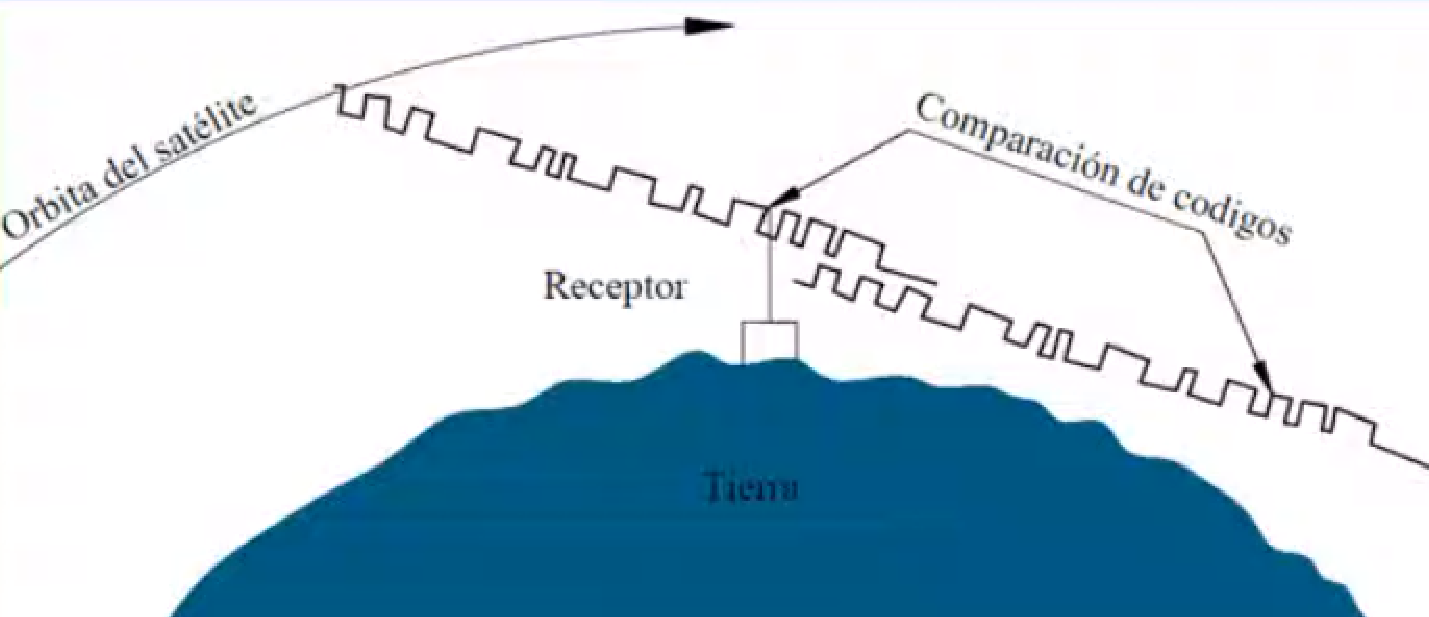
\includegraphics[width=0.5\textwidth]{ta37.pdf}
  \caption{Esquema del método de pseudodistancia}
  \label{ta37}
\end{figure}

\subsubsection{Métodos de posicionamiento}

\begin{itemize}
    \item Posicionamiento absoluto
    \begin{itemize}
        \item Fase de código
        \item Por punto preciso
    \end{itemize}
    \item Posicionamiento diferencial o relativo
    \begin{itemize}
        \item Postproceso
        \begin{itemize}
            \item Estático
            \item Estático rápido
            \item Cinemático
        \end{itemize}
        \item En tiempo real
        \begin{itemize}
            \item Diferencial
            \item Cinemático en tiempo real (RTK)
        \end{itemize}
    \end{itemize}
\end{itemize}

\subsubsection{MPG Estático}

El Método Estático se emplea cuando se requieren altas precisiones, como en el establecimiento de PCA; se pueden emplear al menos dos receptores; uno se sitúa en un PCA previamente establecido con precisión y que se considera como Estación Base (EB) y el otro, en el primer punto desconocido y a posicionar; se hacen mediciones simultáneas desde ambas estaciones a cuatro o más satélites, por un período de tiempo de una hora o más, dependiendo de la longitud de la Línea Base (LB); el receptor sobre la EB, se mueve entonces al segundo punto desconocido, y el otro permanece en el primero para hacer otra sesión de observaciones, considerándolo ahora como EB; se continúa, cambiando el receptor del primer punto desconocido al tercero. permaneciendo el otro en el segundo punto que funciona como EB, y así sucesivamente hasta llegar al último punto a posicionar.

\subsubsection{MPG Estático Rápido}

En el MPG Estático Rápido, se elige un PCA como punto de referencia o EB previamente establecido con el Método Estático y se establecen posiciones absolutas de otros PCA con tiempos cortos de recepción de la señal de satélites, para después corregirlos y ligarlos a una Red Geodésica mediante un trabajo de postproceso y obtener coordenadas X,Y,Z con precisión milimétrica.

\subsubsection{MPG Cinemático}

El MPG Cinemático permite el posicionamiento de varios puntos ubicados alrededor del PB, y es particularmente viable en áreas donde exista una buena visibilidad satelital, lo cual es, a su vez, particularmente posible donde no haya obstáculos, representados por montañas, vegetación o construcciones. Para su ejecución requieren dos receptores, y dos puntos PCA establecidos y posicionados previamente con precisión; un instrumento se estaciona en un PCA definido como Base, y el otro, denominado móvil, ambulante o rover, se estaciona primeramente en el otro PCA por un tiempo del orden de 5 minutos para determinar las ambigüedades, y luego se ubica consecutivamente sobre los puntos cuyas coordenadas se quieren conocer. Usando correctamente este método y con tiempos de recepción con el móvil del orden de 3 minutos, se pueden alcanzar precisiones del orden de 1 o 2 cm en planta y entre 2 y 3 cm en la coordenada Z, de modo que es muy recomendable para el levantamiento de PCD por el Método Topográfico de Radiaciones.

\subsubsection{MPG Cinemático en tiempo real (RTK)}
En el Método Cinemático en Tiempo Real (RTK), además de los receptores de señales satelitales, utiliza un radio de comunicación como medio para transmitir los datos del satélite desde un PCA empleado como referencia hacia el receptor móvil que recibe mediante otro radio; los datos así generados, se procesan conjunta e inmediatamente a su adquisición para resolver las ambigüedades y obtener las coordenadas de los puntos objetivo con precisión milimétrica y mostrarlas al momento en que se lleva a cabo el levantamiento.

Teniendo sólo esa diferencia respecto al Método Cinemático, el Método RTK, tiene las mismas precisiones y aplicaciones que aquel y se está convirtiendo en el método más común para realizar levantamientos GPS de alta precisión en áreas pequeñas y utilizarse en sustitución o complemento en situaciones donde se utilizan estaciones totales.

\subsubsection{Errores y precisión. Clasificación}

\begin{itemize}
    \item Para la navegación o la localización de vehículos, precisiones métricas (del orden de unos cuantos metros) es bastante;
    \item Para el control de maquinaria ya sea en la agricultura o en ingeniería civil es suficiente una precisión centimétrica; y
    \item Para estudios topográficos, lo común es que se requiera precisión milimétrica.
\end{itemize}
La precisión obtenida depende del error estándar del receptor y del método de levantamiento o de medición, que incluye el tiempo de recepción de las señales y de su procesamiento para el posicionamiento.

\begin{itemize}
    \item Asociados a los satélites
    \begin{itemize}
        \item Errores orbitales
        \item Oscilador o reloj
        \item Dilución de la precisión
    \end{itemize}
    \item Relacionados con la propagación de la señal
    \begin{itemize}
        \item Efectos atmosféricos
        \begin{itemize}
            \item Refracción ionosférica
            \item Refracción troposférica
        \end{itemize}
        \item Pérdidas de ciclo
    \end{itemize}
    \item Inherentes con el receptor
    \begin{itemize}
        \item Puesta en estación
        \item Oscilador o reloj
        \item Multiruta
        \item Retardos instrumentales
        \item Variación en el centro de fase
    \end{itemize}
    \item Intencionados para perturbar la señal y disminuir la precisión
    \begin{itemize}
        \item Disponibilidad selectiva
        \item Jamming,Meaconing, Spoofing
        \item Interferencias electromagnéticas
    \end{itemize}
\end{itemize}

\subsubsection{Retrasos ionosféricos y atmosféricos}
Al pasar la señal del satélite a través de la ionósfera, su velocidad puede disminuir, este efecto es similar a la refracción producida al atravesar la luz de un medio a otro de distinta densidad

La ionósfera no introduce un retraso constante en la señal.
La luz sólo tiene una velocidad constante en
el vacío.

\subsubsection{Errores atmosféricos}

Los errores del receptor son causados por ruidos eléctricos durante la transmisión de señales.

Los errores multiruta ocurren cuando una señal transmitida que inicialmente no viajaba hacia un receptor terrestre es reflejada desde otro objeto y entonces recibida. El tiempo de viaje de estas señales reflejadas pueden ser tan grandes que la línea de viaje es errónea en tiempo y rango.

Para reducir los errores debidos al centrado de la antena, el nivel de burbuja de la plomada óptica debe revisarse regularmente y ajustarse si es necesario o usar una plomada de cordón. Los efectos erróneos de una posible corrección en el centrado de la antena puede minimizarse relativamente, en un trabajo de posicionamiento muy cuidadoso.
Se deben tomar las siguientes consideraciones en los errores y precisión:
\begin{itemize}
    \item Los errores en la efemérides de los satélites son incertidumbres que existen en sus órbitas, e implican errores el cálculo de las coordenadas de los satélites del orden de hasta $\pm 20$m
    \item Son errores sistemáticos, los producidos por los relojes tanto de los satélites como de los receptores, los atmosféricos y aquellos relacionados con las trayectorias de los satélites;
    \item Son errores accidentales o aleatorios, las pérdidas de ciclo, los multiruta, la puesta en estación del receptor y en la recepción de las señales por éstos.
\end{itemize}

%\textbf{Establecimiento de un PB y PCA por los métodos y estático rápido y postproceso}
%
%Utilizando un equipo de posicionamiento global por satélite de doble frecuencia modelo GS15 de la marca Leica que consta de dos antenas receptoras, se posicionó por el Método Estático un Punto Base M para un estudio topográfico, en la comunidad Paso de Boca, municipio de Tlalixcoyan, en el estado de Veracruz, y, posteriormente se establecieron por el Método Estático Rápido 14 Puntos de Control y Apoyo denominados M1, M2, M3, M14, en los que se estacionó consecutivamente el segundo receptor empleado como móvil. Para la posterior corrección de las coordenadas del Punto Base M, se utilizó como punto de control el denominado UVER de la Red Geodésica Nacional Activa (del Instituto Nacional Estadística y Geografía, INEGI), lo cual se hizo empleando el software de postproceso Leica GeoOffice; las coordenadas corregidas de la Base M, se utilizaron para corregir las de los puntos establecidos con la antena receptora móvil.

\subsection{Sistemas topográficos con vehículos aéreos no tripulados}

La estación total y GPS no siempre son adecuados con vegetación densa, con accidentes topográficos, condiciones climáticas extremas, esto implica tiempo de trabajo de campo y altos costos, pero los Drones pueden ser una buenas alternativa

\begin{definition}[Vant]
    Un vehículo aéreo no tripulado (VANT), (Unmanned Aereal Vehicle) o comúnmente DRON es una aeronave que es capaz de volar a control remoto o bien a través de un programa preestablecido mediante un software especial.
Se constituye en el Componente de Transporte del sensor que adquiere la información que al procesarse permite posicionamiento de puntos sobre la tierra y en conjunto conforman un Sistema Topográfico con Vehículos Aéreos No Tripulado (SITVANT)
\end{definition}

El diseño de los VANT tiene una amplia variedad de formas, tamaños, configuraciones y características.

Miden con equipos modernos como GPS, sensores infrarrojos, RADAR, SONAR y LIDAR y cámaras fotográficas de alta resolución y controles remotos de precisión

Segmento de Vuelo (SV): formado por el Vehículo Aéreo y los sistemas de recuperación (aterrizaje sobre ruedas o patines, red, cable y paracaídas).

Segmento de Tierra (ST): Estación de Control en tierra que recibe la información enviada por el dron y les da indicaciones.

\subsubsection{Tipos de VANT por su motor}

\begin{itemize}
    \item \textbf{.De ala fija} Alcanzan distancias de hasta 60 km y una hora de vuelo; pueden superar los 500 m de altura y velocidades de 50 y 70 km/h; los despegues se realizan desde una plataforma y aterrizan contra el suelo; los sensores o cámara se colocan fijos y en posición cenital.\footnote{Especialmente versátiles para cartografía y toma de ortoimágenes.}
    \item \textbf{De ala rotativa}. Menor autonomía 30 minutos de vuelo y distancias menores de 10 km; tienen entre 4 y 8 hélices de longitudes de hasta un metro; pueden girar sobre sí mismos en distancias muy cortas, lo que los hace especialmente versátiles para trabajos verticales. Despegan y aterrizan verticalmente. \footnote{Igualmente pueden portar todo tipo de cámaras.}
\end{itemize}

Los usos de los VANT en ingeniería, son la Adquisición de imágenes, para producir ortofotos y MDE en tiempo real,
Inspección de infraestructura, Gestión y control de riesgos, Exploración de zonas de difícil acceso,
Monitoreo y control de tráfico, Combate de enfermedades en zonas agrícolas y forestales.

Con un SISVANT, el terreno se escanea con una cámara o sensor instalado sobre el
VANT, obteniéndose imágenes estereoscópicas, que se procesan en gabinete para obtener un modelo 3D con resolución centimétrica y una precisión de entre 1 y 5 cm según se requiera, lo cual es muy apropiado para estudios topográficos de cuencas hidrológicas, vasos de almacenamiento y zonas agrícolas y podría no ser suficiente para el levantamiento de las boquillas, rutas para vías de comunicación y zonas
Por lo tanto, la otra componente de los SITVANT es el de medición y procesamiento que, a su vez, puede estar conformado por:

\begin{enumerate}
    \item cámaras digitales, que en conjunto con los elementos para el procesamiento de las imágenes digitales conforman la fotogrametría digital;
    \item Sensores LÁSER;
    \item Sensores de RADAR; y
    \item Sensores LIDAR
\end{enumerate}

\subsubsection{Fotogrametría}

El terreno se escanea con una cámara instalada sobre él, obteniéndose imágenes estereoscópicas, que se procesan para obtener un modelo 3D con resolución centimétrica y una precisión de entre 1 y 5 cm. Tiene buena precisión, seguridad, mayor cobertura, tiempo reducido y más información

La fotogrametría digital surge como consecuencia del gran desarrollo de la computación, que permitió realizar todos los procesos fotogramétricos utilizando computadoras y software especializados, posibilitando la generación y uso las imágenes incluyendo y extrayendo una amplia gama de información, como modelos digitales de elevación del terreno, ortoimágenes, estéreo-imágenes, visualización tridimensional del terreno, perfiles transversales, etc., con mayor rapidez, facilidad relativa y precisión. 

La simplicidad del formato digital posibilita y facilita que el operador realice manualmente la restitución (supervisada) o bien que lo haga la computadora en forma automática (no supervisada); en cualquier caso, la salida puede ser en dos formatos, el ráster o el vectorial. La generación de datos empieza con la toma de la imagen sea cual sea su origen: fotografías aéreas escaneadas en un sistema de gran precisión o bien imágenes de satélite capturadas con sensores como SPOT o Landsat o, imágenes digitales capturadas con cámaras digitales.

Cuando se utilizan drones para un levantamiento, cambia la forma de trabajar; no es necesario definir una serie de Puntos para Configuración y de Detalle para su levantamiento o posicionamiento, sino que se levanta en campo y se modela en gabinete de una vez toda el área de trabajo, y la posición de los puntos necesarios o útiles se hace determinando sus coordenadas con el empleo del modelo; esto también tiene la ventaja de que se elimina la necesidad de tener que volver a hacer trabajo de campo si hacen falta nuevas medidas.

Para el trabajo de campo, el dron se debe programar apoyados en Puntos de Control y Apoyo que se deben establecer en tierra en cantidad suficiente y ubicación conveniente que permitan calcular y corregir los errores de restitución con el modelo estereoscópico generado, y de modo que se haga un barrido del terreno con rutas paralelas de vuelo.

La cámara deberá de ir tomando fotografías en lapsos programados de tiempo y las imágenes se deben ir etiquetando con su posición georeferenciada.

\subsubsection{Procesamiento y productos de las imágenes}

Modelo Digital de Elevaciones (MDE), es la representación gráfica y matemática de los valores de altitud de los puntos del terreno, que permite caracterizar las formas del relieve y los elementos u objetos presentes en el mismo

Y un Modelo Digital de Superficie (MDS) representa las elevaciones sobre el nivel del mar de las superficies reflectantes de árboles, edificios, obras de infraestructura y otras características elevadas sobre el nivel de la superficie del terreno.

Las ventajas son muchas, entre ellas:

\begin{itemize}
    \item a%%%%%%%%%%%%%%%%%%%%%%%%%%%%%%%%%%%%%%%%%%%%%%%%%%%%%%%%%%%%%%%%%%%%
    %%%%%%%%%%%%%%%%%%%%%%%%%%%%%%%%%%%%%%%%%%%%%%%%%%%%%%%%%%%%%%%%%%%%
    %%%%%%%%%%%%%%%%%%%%%%%%%%%%%%%%%%%%%%%%%%%%%%%%%%%%%%%%%%%%%%%
    \item Teniendo los softwares adecuados y los equipos apropiados, se tiene una gran facilidad de visualización y manipulación para encontrar los puntos homólogos y para su análisis y el procesamiento de restitución.
    \item Los procesos de análisis, interpretación, restitución y generación de resultados son automáticos o pueden automatizarse, incrementando la velocidad de su ejecución y con ello, la productividad del trabajo de los operadores y del equipo.
    \item Se reducen los errores instrumentales derivados del equipo de toma de las imágenes y aquellos resultantes de su procesamiento, con lo que además se obtienen precisiones milimétricas en la obtención de las coordenadas de los puntos.
    \item Salida digital de la información, lo que permite su manejo para la elaboración de planos específicos y/o para su empleo en el proyecto de obras o el diseño de sistemas
    \item El almacenamiento, la reproducción y la distribución de las imágenes originales y de los archivos generados como resultados o productos es más fácil y rápido.
\end{itemize}
En resumen y como resultado de múltiples experiencias, se puede señalar que los drones se están utilizando para realizar trabajos topográficos con amplias ventajas, pues para muchos casos resulta mucho más económico en tiempo y costo, que comprar información LIDAR, contratar estaciones topográficas o rentar helicópteros para tomas aéreas considerar y. se recomienda la calidad/precio, pues relación mientras más precisión se necesite, la inversión monetaria será más Grande

Tiene también unas desventajas:

\begin{itemize}
    \item El equipo para la toma de las imágenes es especializado y, por tanto, el personal para su ejecución también debe serlo.
    \item El tratamiento o procesamiento de las imágenes requieren de software especiales y de los equipos con las mejores características de capacidad de procesamiento y almacenamiento, y de velocidad y resolución apropiadas.
    \item Los equipos y software tienen costos comparativamente altos.
\end{itemize}

\subsection{SistVant con sensores LiDAR}

\begin{definition}[LiDAR]
    El término LIDAR significa en el idioma inglés Light Detection and Ranging y para fines prácticos y de la Topografía, se puede traducir como medición de distancias por emisión y detección de luz láser, que corresponde al rango de la luz visible (por ejemplo el color azul con 5.32 mm de longitud, para penetración de cuerpos de agua) o regiones del infrarrojo cercano (por ejemplo 1.64 mm por su sensibilidad a la vegetación y libre de dispersión atmosférica).
\end{definition}
Los sensores LiDAR son del tipo activo, es decir que emiten su propia señal, y difieren en muchos aspectos de los radares de microondas, en principio por las diferentes regiones del espectro que utilizan.

Los equipos LIDAR empleados para estudios topográficos conforman un Sistema Topográfico con Vehículos Aéreos No Tripulados (SITVANT), al instalarse sobre un dron que realiza un vuelo cuya altura, velocidad y ruta se definen con precisión para transmitir su señal como pulsos de luz de amplitud y frecuencia conocida y medir con alta precisión el tiempo que tarda una porción de los mismos, en retornar al instrumento emisor después de hacer contacto con los objetos cuya ubicación se desea conocer y rebotar, mismo que al estar geoposicionado con el apoyo de un SPGS permite la determinación de sus coordenadas geográficas.

Para conocer las coordenadas de cada punto sensado se necesita la posición georeferenciada y precisa del emisor y el ángulo de inclinación del sensor en cada instante de medición, para lo cual el SITVANT se integra también de un SPGS y de un Sistema de Navegación Inercial (INS), de modo que al calcular la distancia sensor-terreno con el principio del distanciómetro, hace posible la determinación de las coordenadas georeferenciadas y precisas del punto del terreno. El esquema de la figura 2.88 ilustra el concepto de medición del SITVANT con sensores LİDAR.
\begin{figure}[h!]
\centering
  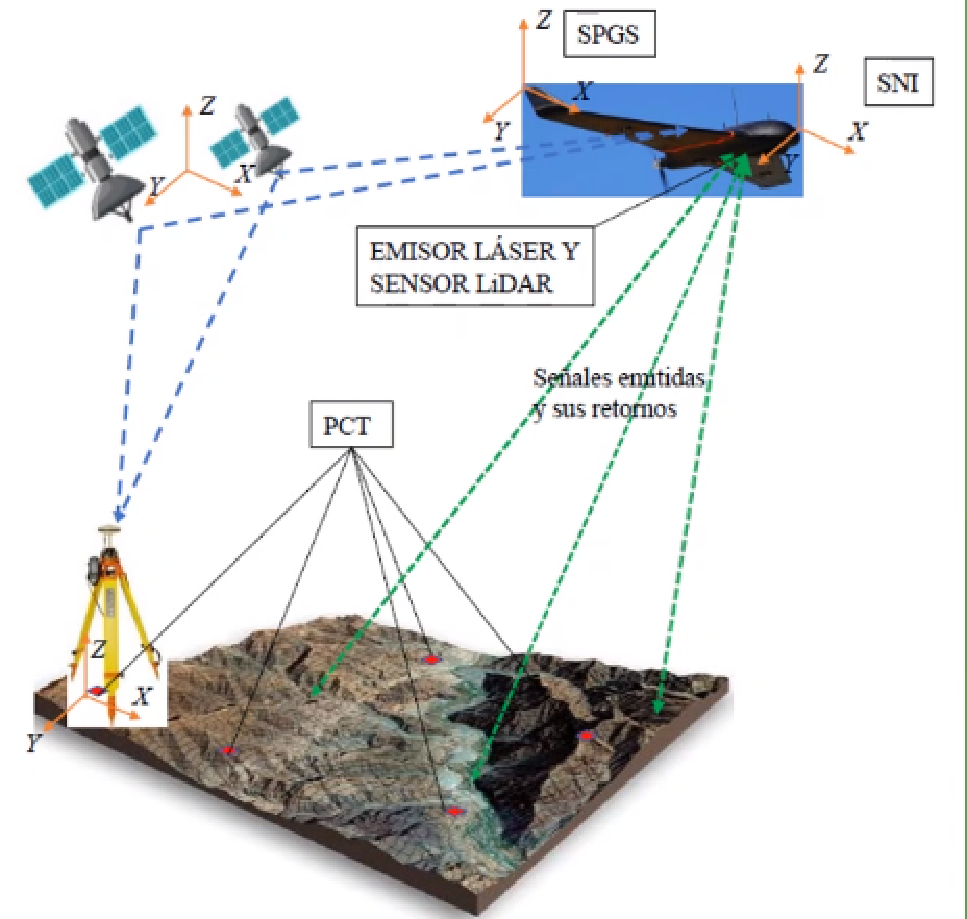
\includegraphics[width=0.5\textwidth]{ta38.pdf}
  \caption{Principios de funcionamiento}
  \label{ta38}
\end{figure}
Dada la multiplicidad y velocidad de emisión y recepción de la señal LÁSER, el SITVANT-LiDAR obtiene una nube de puntos de una amplia área del terreno objeto de estudio al realizar un escaneado que combina dos movimientos: uno longitudinal definido por el vehículo de transportación y otro transversal generado por el movimiento de sensor que recibe el haz de luz LÁSER una vez que es rebotado por el objeto a posicionar y que viaja a la velocidad de la luz.
\begin{figure}[h!]
    \centering
      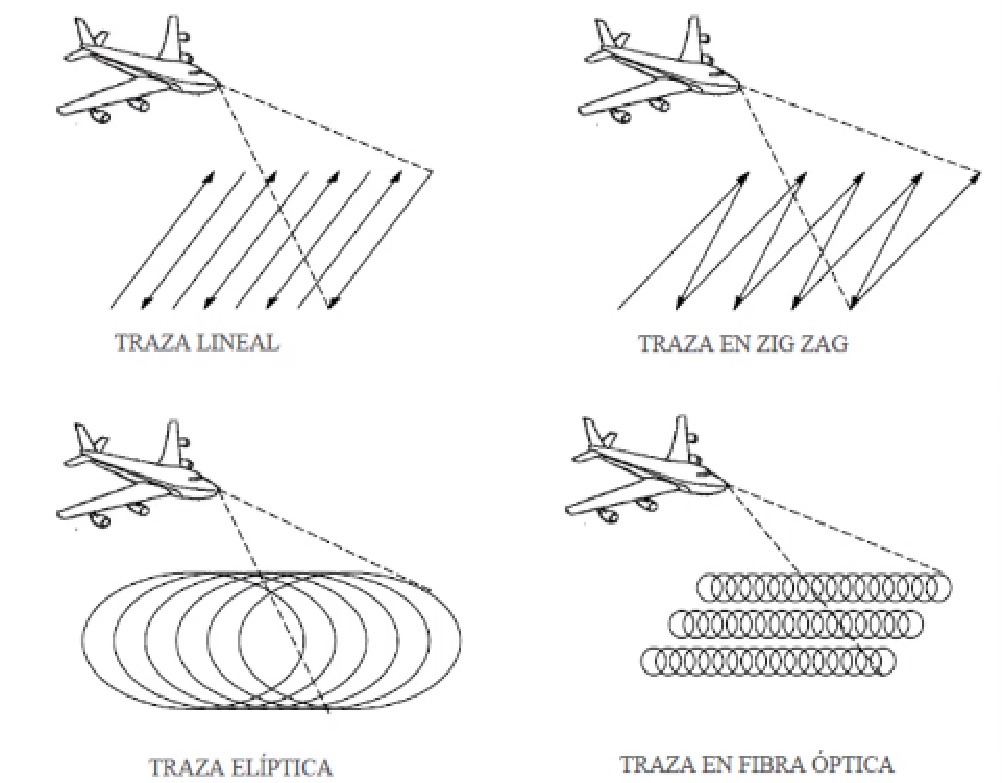
\includegraphics[width=0.5\textwidth]{ta39.pdf}
      \caption{Patrones de captura de imágenes}
      \label{ta39}
    \end{figure}

\subsubsection{Componentes del SITVANT}

\begin{itemize}
    \item \textbf{Escáner láser aerotransportado} (ELA), que es propiamente el equipo LiDAR que emite pulsos de luz láser e infrarroja que sirven para determinar la distancia entre el sensor y el terreno u objeto a posicionar.
    \item \textbf{Sistema de Posicionamiento Global por Satélite}, mediante el que se da posición precisa del receptor en el VANT y la de uno o varios Puntos de Control Terrestre (PCT) mediante el conocimiento de SUS tres coordenadas geográficas UTM determinadas con métodos diferenciales y de post proceso para obtener precisiones milimétricas,
    \item \textbf{Sistema de Navegación Inercial} (SNI), que genera y proporciona información precisa en tiempo y espacio sobre la trayectoria del avión y del sensor en su movimiento transversal.
    \item \textbf{Cámara de Video Digital} (CVD) que, permite obtener una imagen digital, que resulta de mucha valía para la mejor interpretación de los resultados, y puede montarse junto al ELA o ser parte del mismo, pues las imágenes en color verdadero se conforman de la integración de las reflectancias de los colores rojo, verde y azul (RGB por sus iniciales en el idioma inglés).
    \item \textbf{Medio o vehículo aéreo}, que (como cualquier VANT) bien puede ser un pequeño avión o un diminuto helicóptero; el primero se prefiere cuando se quiere privilegiar la productividad y el área de estudio es grande, y el segundo se emplea mayormente cuando se quiere mayor densidad de puntos, debido a que éste puede volar más lento y a menor altura.
\end{itemize}

%\subsubsection{Clasificación del SITVATN}
%
%Por el tipo de señal
%\begin{itemize}
%    \item 
%\end{itemize}

Por el tipo de escaneo

\begin{figure}[h!]
    \centering
      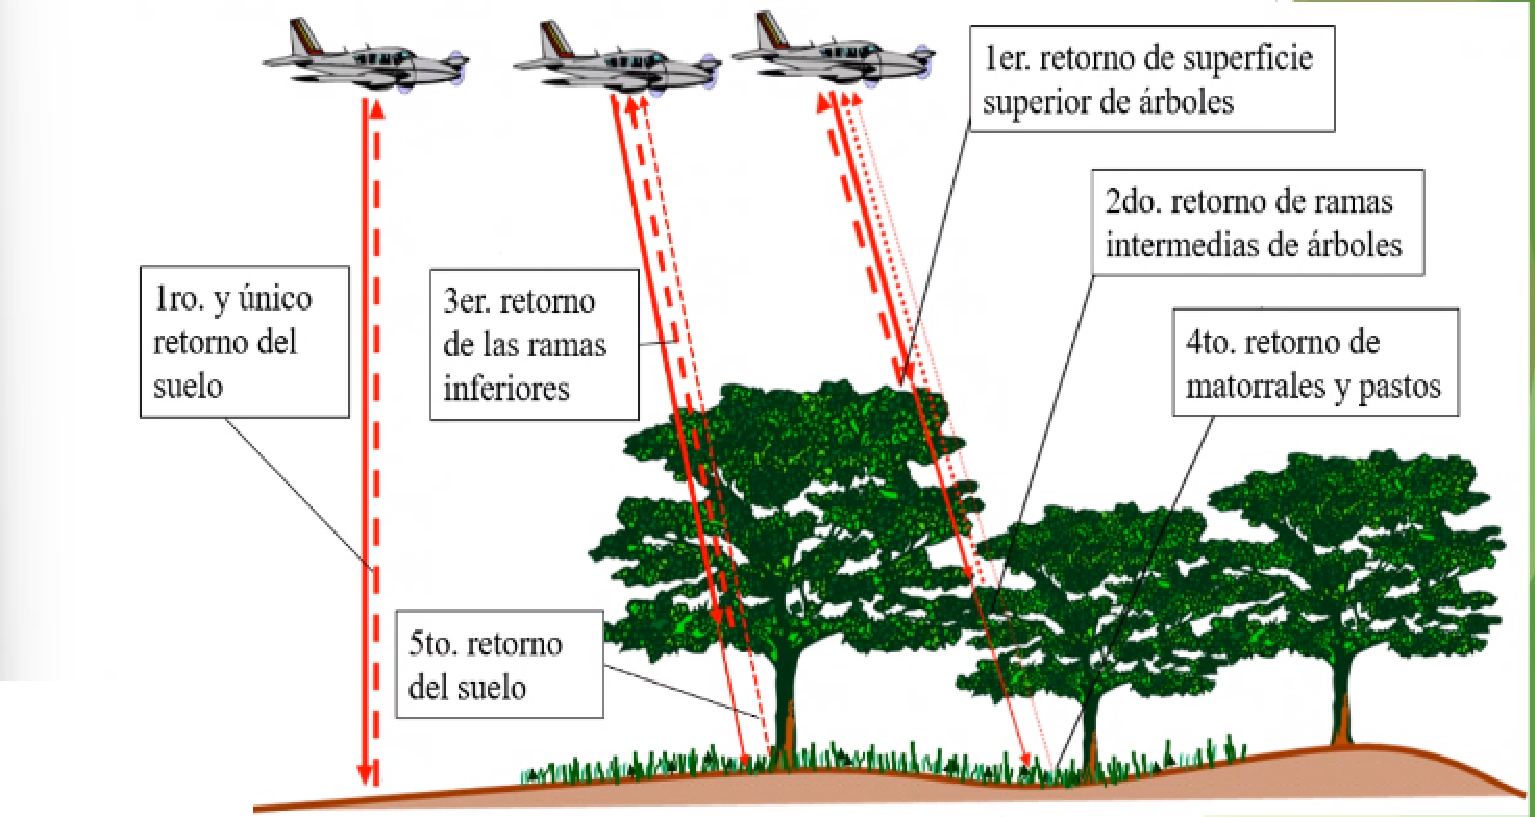
\includegraphics[width=0.5\textwidth]{ta400.pdf}
      \caption{Sensado de los retornos}
      \label{ta400}
    \end{figure}
    La colección total de los retornos LIDAR de una región, pueden examinarse para separarlos de entre los que se originaron sobre un nivel especifico de los que se originaron por debajo del primero, pudiéndose formar un tipo de procesos de filtración o discriminación para separar los retornos del suelo de los que no son retornos de él, y con un análisis adicional, se separa la superficie del terreno, de la estructura y cubierta vegetal que tiene sobre ella. De este modo es posible calcular de forma muy precisa la altura de los árboles, los edificios y obtener la configuración del terreno

    Los sistemas LIDAR, proveen datos espaciales de alta precisión y mediciones directas de elevación superficial, con detalle y precisión usualmente asociadas solamente con los levantamientos fotogramétricos. Sus aplicaciones principales están enfocadas por ello también a regiones urbanas, en las cuales se requiere de información detallada respecto a la densidad de los edificios, sus niveles y huellas. De ahí que los datos LIDAR se pueden usar para la planeación y proyecto de carreteras, sistemas de tuberías, líneas de comunicación inalámbrica, y otras similares en regiones urbanas, así como para estudiar la configuración, estructura y densidad de áreas forestales, con lo que se pueden elaborar mapas para su descripción y análisis

\begin{enumerate}
    \item Planeación. Se define y precisa el área de trabajo con la ayuda de imágenes satelitales y/o mediante vuelos en helicóptero o avioneta según su extensión y condiciones, identificando sus límites, forma y magnitud, así como su cobertura, definida por edificaciones, construcciones, vegetación, vías de comunicación, etc. Con esta información se plantea el tipo de VANT y de sensor LIDAR que se empleará y las rutas generales y tiempos para la ejecución de los trabajos. Se proponen asimismo el número y ubicación general de los Puntos de Control Terrestre (PCT).
    \item Recorrido de campo y establecimiento de Puntos de Control Terrestre. Se identifican los sitios más adecuados y convenientes para la localización de los PCT y se establecen físicamente mediante un monumento, un cincel O una varilla, y técnicamente, determinando sus coordenadas XYZ UTM, empleando un equipo de posicionamiento global y un Método que proporcione la precisión requerida, que para fines topográficos debe ser del orden de milímetros.
    \item Programación del vuelo. Con el uso de un software especial y adecuado, se realiza el plan de vuelo, definiendo las rutas necesarias y sus direcciones, la velocidad y la altura. Se debe precisar, asimismo, el número de horas y días en su caso, del vuelo y las características de las señales láser emitidas y recibidas como pulsos electromagnéticos que son las entidades básicas para la medición.
    \item Ejecución del vuelo. Consiste en la realización del vuelo o de los vuelos programados, para generar la información producto del sensado de la superficie en estudio con el sensor LIDAR Y almacenarla en un archivo de extensión LAS, según se describe enseguida.
\end{enumerate}
Los productos LiDAR generados son los siguientes:

\begin{itemize}
    \item Nube de puntos irregular correspondiente a los puntos LiDAR originales; se entregan como información LIDAR bruta o cruda, clasificada generalmente en una sola categoría definida por default.
    \item Nube de puntos clasificada; que se obtiene aplicando algoritmos de clasificación automática a la nube de puntos bruta y clasificando cada punto de acuerdo a su posición relativa con respecto a los puntos más cercanos dentro de la nube. Las clases pueden ser suelo, vegetación (alta, media y baja, por ejemplo), edificios, traslape entre pasadas, líneas eléctricas, puentes, ruido/errores, etc.
    \item Imagen de intensidades. Se obtiene a partir de la amplitud de la señal que retorna al sensor después de rebotar en la superficie objetivo, según el número de rebote, y permite realizar distinciones entre superficies.
\end{itemize}

El trabajo de gabinete,

se hace con el empleo de los software o aplicaciones especiales existentes en el mercado libre o

suministradas por los fabricantes de los equipos que contienen algoritmos especializados y sofisticados, y consiste en varias intervenciones automáticas (con algoritmos de clasificación etc.) e intervenciones
de superficies, filtrado automático de errores,manuales

Las ventajas de los SITVANT-LiDAR:
\begin{itemize}
    \item Utilizan pulsos de luz de la banda del infrarrojo cuyas características hacen posible su uso de noche y para la captura de datos batimétricos.
    \item El sensor LiDAR es del tipo activo, y tiene la posibilidad de penetración de cada pulso emitido a través de hojas o cubiertas delgadas, permitiendo la captura de hasta 5 retornos o rebotes de cada pulso, y de medir la elevación del terreno en zonas completamente cubiertas por la vegetación, con precisión vertical milimétrica.
    \item Un solo equipo LIDAR puede generar del orden de 300,000 señales por segundo y recoger varios ecos o rebotes para el mismo haz luminoso, lo que a su vez, hace posible levantar grandes áreas en tiempos relativamente cortos, lo que se puede traducir a una mayor productividad respecto a otros sistemas
    \item No requiere de hacer anotaciones y su procesamiento posterior es completamente automatizado, si bien, como se ha dicho se debe tener dominio de herramientas tecnológicas y metodológicas empleados.
    \item La precisión centimétrica e incluso milimétrica, y su mayor resolución, así como la obtención de datos con estas características bajo la cubierta vegetal
    \item Aún en condiciones de amplia cobertura, como la selva tropical, es posible crear modelos digitales del terreno más precisos que las ortofotos o las ortoimágenes.
\end{itemize}

Las desventajas por otra parte son:

\begin{itemize}
    \item Los componentes del sistema para el trabajo de campo son varios y requieren su adquisición, integración y acoplamiento perfecto para su adecuado y eficaz funcionamiento.
    \item Requerimiento de equipos y software especializados para el procesamiento de la información de campo y para la generación de los productos finales.
    \item Altos costos iniciales comparativos con los demás sistemas que proporcionan información planialtimétrica.
    \item Se requiere capacitación especializada de personal tanto de campo como de gabinete.
\end{itemize}    

\section{Estudios para obras de almacenamiento de agua}
\begin{enumerate}
    \item Una presa o bordo de almacenamiento de agua es una obra civil e hidráulica que consiste de:
    \item Una cortina de concreto, mampostería o de materiales graduados, que es la obra de retención del agua.
    \item Una obra de excedencias para desalojar los excedentes que se generen por una avenida máxima una vez que el almacenamiento esté lleno
    \item Una obra de toma para extraer de manera programada y controlada el agua para su uso, aprovechamiento o control
\end{enumerate}
Importancia y objetivos: La finalidad de una obra de almacenamiento puede ser una o más de las siguientes:
\begin{itemize}
    \item Control de avenidas.
    \item Potable, público urbano o doméstico
    \item Riego agrícola
    \item Generación de energía eléctrica
\end{itemize}
Para el proyecto, diseño, construcción y operación de obras hidráulicas de almacenamiento, se deben realizar una serie de estudios, para obtener la información necesaria:

\textbf{Hidrológicos}: Para conocer los volúmenes posibles de almacenar y definir capacidad de la obra.

\textbf{Geotécnicos}: para determinar las características mecánicas del sitio de la obra y de los materiales para la obra.

\textbf{Agrológicos}; para determinar los requerimientos de agua para riego.

\textbf{Socioeconómicos}: Para determinar los costos y beneficios de la obra

\textbf{Meteorológicos}: Para estimar los volúmenes precipitados y los escurridos.

\textbf{Geológicos}: Para conocer las condiciones regionales de la zona de construcción y definir su viabilidad.

\textbf{De tipo constructivo}: Para definir la disponibilidad de materiales y los procedimientos de construcción.

\textbf{Topográficos}. Para determinar la magnitud de la obra y sus estructuras y servir de base para los demás estudios

Los estudios topográficos se realizan para el área de la boquilla (que es donde se proyectará y construirá la obra y sus estructuras), del vaso de almacenamiento (donde se producirá el almacenamiento) y de la cuenca de captación (donde se generan los escurrimientos).

\begin{figure}[h!]
    \centering
      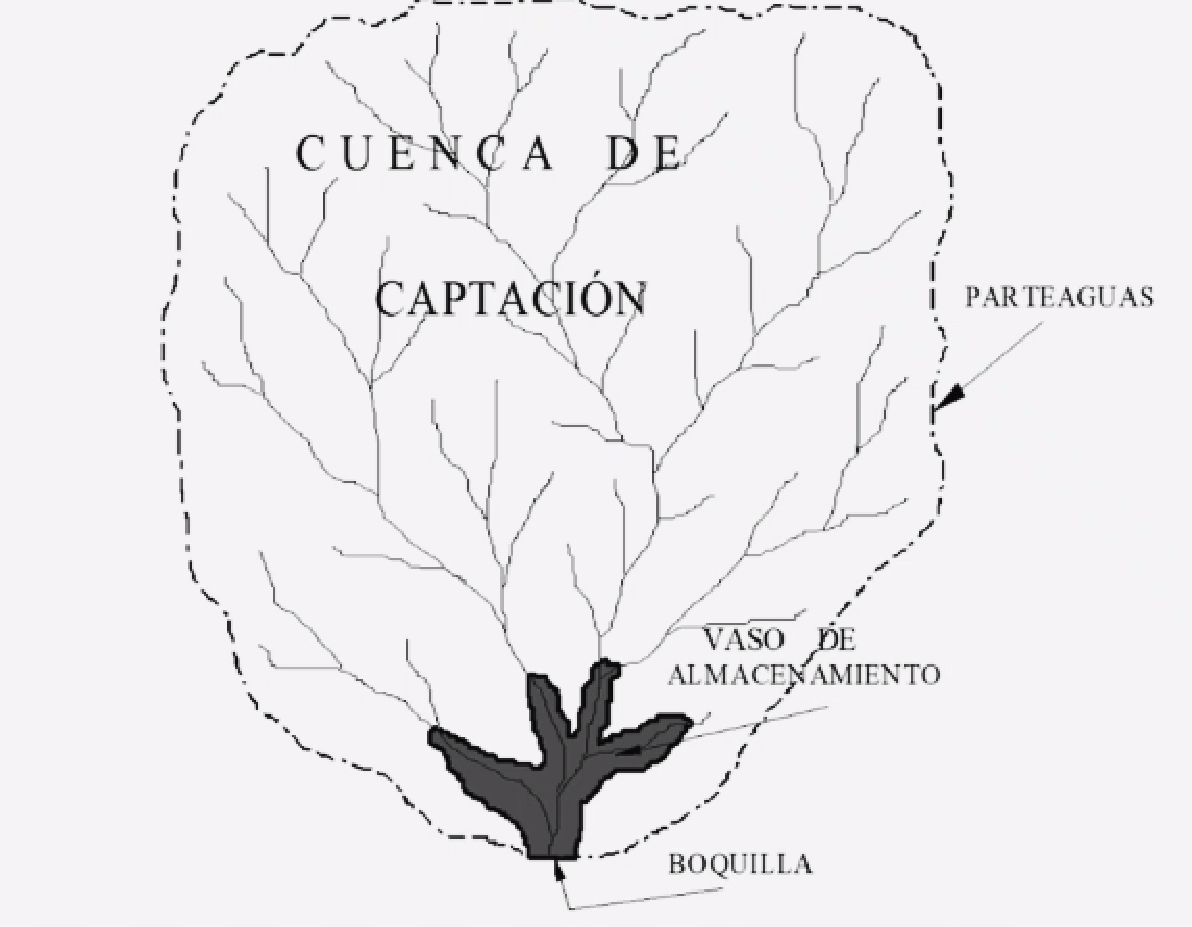
\includegraphics[width=0.5\textwidth]{ta40.pdf}
      \caption{Cueca}
      \label{ta40}
\end{figure}

\subsection{Levantamiento de la boquilla}

\begin{enumerate}
    \item Obtener un plano lo suficientemente detallado y a una escala adecuada, para proyectar en él todas las estructuras hidráulicas que conformarán la Obra de Almacenamiento, tales como, la propia cortina, la obra de excedencias y la obra de toma.
    \item  Elaborar un plano detallado, que sirva de apoyo para los estudios geológicos y de mecánica de suelos de la propia Boquilla, que a su vez, permitirán definir la factibilidad de la obra desde estos puntos de vista.
    \item  Establecer los suficientes Puntos de Control y Apoyo que permitan dar "líneas y niveles" durante la construcción de la obra.
\end{enumerate}

\subsection{Levantamiento de la boquilla}

Para boquillas pequeñas, podemos realizar los siguientes pasos:

\begin{enumerate}
    \item Se localizan dos PCA, uno en cada ladera 0 margen de la boquilla, aproximadamente a la misma elevación y mayor que la del embalse máximo probablę, y de modo que definan lo más adecuadamente posible los extremos del eje probable de la cortina. A dichos Puntos, de ordinario, se les denomina con las letras A y B para las márgenes izquierda y derecha, respectivamente.
    \item La línea A-B, constituida como el eje probable de la obra, se orienta magnética o astronómicamente según se considere y de acuerdo con la importancia o más propiamente, con la magnitud de la obra.
    \item Haciendo estación en A y visando el Punto B, se traza el eje, alineando con tránsito o teodolito, y midiendo como cadenamientos las distancias desde A con cinta (o con distanciómetro), con intervalos regulares cada 3, 5, 10 o 20 m, según la topografía del terreno y/o en los cambios de pendiente; estableciendo como punto particular el correspondiente al fondo del cauce. Todos los puntos se nivelan con nivel montado por Nivelación de Perfil partiendo del Punto A, al que se le asigna Z arbitraria si el trabajo no es de importancia o bien, se le determina su elevación sobre el nivel medio del mar, cuando se considere necesario.
    \item Para el levantamiento de Puntos para Configuración y de Detalle, se sigue el Método de Puntos Aislados empleando tránsito o teodolito y estadal o estación total y haciendo estación en los PCAA y B.
\end{enumerate}

Para boquillas grandes, podemos realizar los siguientes pasos:

Son aquellas boquillas que no siguen la metodología descrita en el inciso anterior.

El trazo del eje probable es similar para ambos casos, de manera que los los puntos 1, 2 y 3 para el levantamiento de Boquillas pequeñas, son iguales con la salvedad de que, si el eje probable es muy grande o no siguiera una sola dirección en toda su longitud, y deberán hacerse los cambios de aparato necesarios para continuar con el trazo.

\begin{enumerate}
    \item Se establecen Poligonales que cierren las anteriores Poligonales Abiertas, tanto en sus extremos aguas-arriba como en los de aguas abajo.
    \item Si aún quedan áreas que no se pudieran levantar se trazan Poligonales internas que permitan localizar PCA adicionales para el levantamiento de dichas áreas.
    \item Todos los PCA establecidos, se nivelan con nivel montado por Nivelación Diferencial.
    \item La configuración y el levantamiento de detalles se hace con tránsito, teodolito y estadal o con distanciómetro o estación total, por el Método de Radiaciones, y capturando información suficiente para dibujar configuración de la Boquilla con curvas de nivel equidistantes verticalmente 1.00 m.
\end{enumerate}

\subsubsection{Trabajo en gabinete}

El trabajo de gabinete consiste básicamente en obtener un perfil de la Boquilla por el eje probable y la configuración del terreno en el área en que ésta se localiza.

El dibujo del perfil se hace con escala mayor en el eje vertical que en el horizontal, en una razón 5:1, para mostrar con mejor claridad los cambios de pendiente en el perfil.

Para la configuración, se calculan las coordenadas de todos los PCD levantados, previa comprobación y compensación de las Poligonales establecidas, y se dibujan curvas de nivel a cada 1.0

\begin{figure}[h!]
\centering
  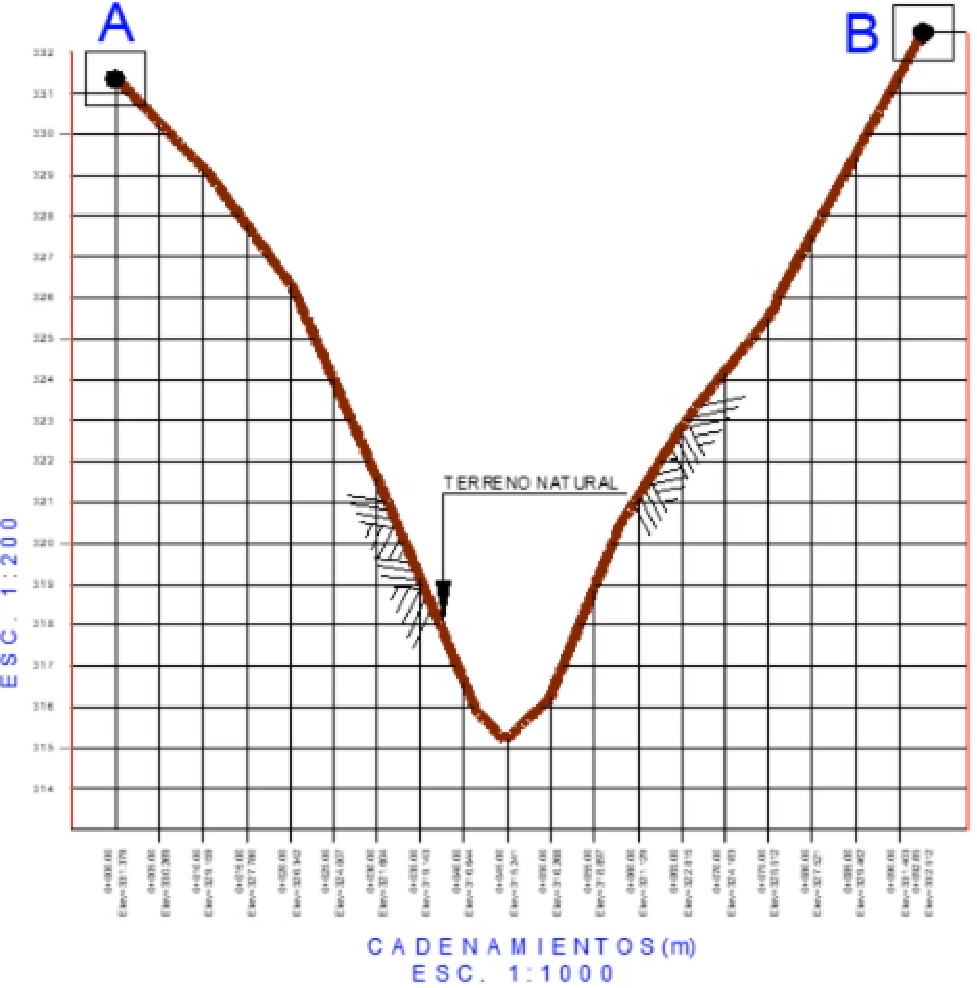
\includegraphics[width=0.5\textwidth]{ta41.pdf}
  \caption{Ejemplo de un cadenamiento en la presa La Zarcita Tejupilco, Estado de México}
  \label{ta41}
\end{figure}
\begin{figure}[h!]
\centering
  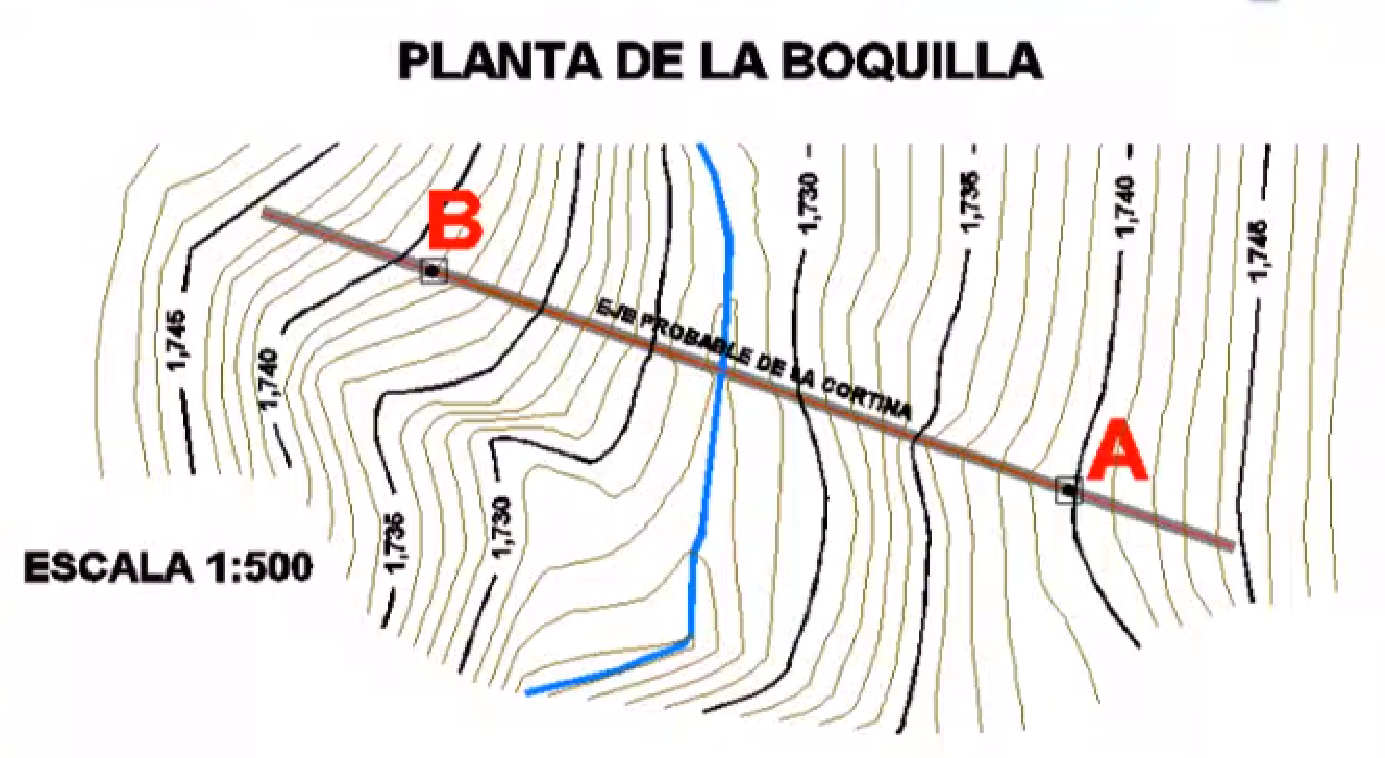
\includegraphics[width=0.5\textwidth]{ta42.pdf}
  \caption{Esquema de la configuración del terreno}
  \label{ta42}
\end{figure}

\begin{align}
    \text{Tolerancia lineal } TL = \frac{1}{10,000}\\
    \text{Tolerancia angular } TA = a \sqrt{n} \\
    \text{Tolerancia de nivel } TN = 8.4 \sqrt{k} \\
\end{align}

\subsubsection{Especificaciones para los planos}

Se debe elaborar un plano en el que se incluya un dibujo de la configuración del terreno a una escala de entre 1: 500 y 1: 1,000, según ésta sea pequeña o grande, respectivamente, y con curvas de nivel equidistantes, invariablemente cada 1.00 m.

En el mismo dibujo se debe incluir el SPLCA y en un cuadro adicional, las tres coordenadas de todos los Puntos de Control y Apoyo. Se debe anexar también, el perfil de la Boquilla por el eje probable de la cortina y un croquis de localización.

\begin{figure}[h!]
\centering
  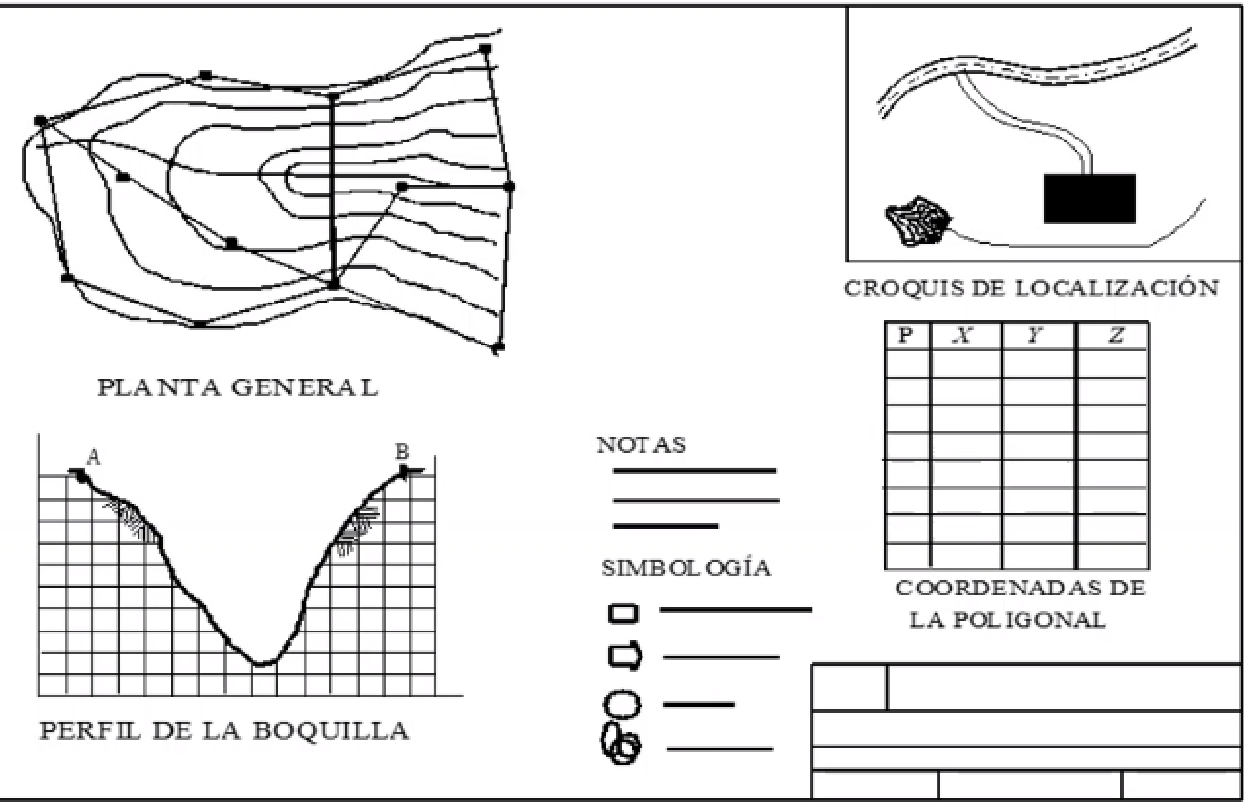
\includegraphics[width=0.5\textwidth]{ta43.pdf}
  \caption{Especificaciones de los planos topográficos}
  \label{ta43}
\end{figure}

\subsection{Levantamiento del vaso de almacenamiento}

El Vaso de Almacenamiento es el área de la parte baja de la Cuenca, aledaña a la boquilla y aguas-arriba de ésta, donde se alojarán los escurrimientos que genere la cuenca, una vez que se construya la obra en la boquilla y se produzca el embalse.

El tamaño del Vaso, medido tanto por el área cubierta o inundada, como por el volumen almacenado, depende de la altura de la cortina, por lo tanto, se debe obtener su Configuración para conocer su capacidad de almacenamiento y su área inundada bajo diversas alternativas de altura de la cortina.

\begin{enumerate}
    \item Determinar el área de embalse o área inundada a diferentes elevaciones de la cortina, lo cual se gráfica en la curva de elevaciones áreas.
    \item Determinar la capacidad de almacenamiento a diferentes alturas de la cortina, lo cual se expone en la denominada curva de elevaciones-capacidades.
    \item Obtener un plano topográfico que sirva de apoyo geológico que a los estudios efectuarán se posteriormente, para determinar el grado de impermeabilidad del vaso.    
    \item Levantar con precisión todos los datos relativos a las propiedades comprendidas dentro del nivel de embalse máximo probable, para determinar las indemnizaciones correspondientes, en su caso.
\end{enumerate}
La capacidad de almacenamiento del Vaso a diferentes elevaciones de la cortina, permitirá en la etapa de proyecto, definir la altura más apropiada para ésta.

Por supuesto, que en esta etapa, es necesario considerar también el volumen de material para construir la cortina, junto con la capacidad de almacenamiento del Vaso (relación volumen almacenado/volumen de obra). Además, el conocimiento de la relación elevación de la cortina/capacidad de almacenamiento. permitirá definir la elevación de la obra de toma y la del vertedor.

Por otra parte, la determinación del área de embalse a diferentes elevaciones de la cortina, junto con la curva de elevaciones-capacidades, proporcionará información muy importante para cuando la obra ya se encuentre en operación.

Se pueden seguir diversos Procedimientos y Métodos, dependiendo de si se trata del levantamiento preliminar 0 del definitivo, de la magnitud del vaso y de su cubierta vegetal, así como del equipo topográfico disponible.

El Estudio Topográfico puede ser:

\textbf{Preliminar}: Se hace para grandes cuando hay más de una alternativa de área para el conjunto BOQUILLA-VASO y debe elegirse la mejor, para lo cual se hacen estudios expeditos y aproximados.

\textbf{Definitivo}: Se hace para la alternativa definitiva y con el mayor detalle y precisión recomendados para el caso y para cubrir los objetivos

La SRH recomendaba las siguientes opciones para los ESTUDIOS PRELIMINARES:

\begin{itemize}
    \item Poligonal Abierta por el Cauce Principal y Secciones Transversales Ampliamente Espaciadas.
    \item Poligonal Abierta por el Cauce Principal y Radiaciones Configuración Tosca. para configuración tosca
    \item Método de obtención directa de curvas de nivel
\end{itemize}

Actualmente se recomienda realizar y emplear los equipos y sistemas modernos como GPS y SITVANT con sensores LIDAR, y levantar o posicionar PCD por el Método de Radiaciones en cantidad suficiente y distribución conveniente (cambios importantes de pendiente) de modo que se pueda dibujar la configuración del vaso con curvas de nivel cada 2.5 m; o en obras muy grandes a cada 5.0 m.

Para los estudios definitivos se establece en primer lugar, un Sistema de Puntos y Líneas de Control y Apoyo para, posteriormente y apoyados en él, levantar los Puntos para Configuración y de Detalle. En cualquier caso, el sistema debe ligarse con los PCA de la Boquilla.

\emph{Si se establece un SPLCA con Procedimientos Planimétricos primeramente.}

En obras muy pequeñas como son las de abrevadero, los PCA pueden ser los mismos de la Boquilla y si acaso agregar uno a dos PCA a partir de ellos.

En obras grandes, se establecen una combinación de Poligonales Abiertas y Cerradas, a partir de los PCA de la Boquilla y por las partes bajas de los cauces, localizando y distribuyendo los PCA del modo más conveniente para el levantamiento posterior de los PCD.

Apoyados en estas Poligonales principales, se establecen poligonales auxiliares siguiendo caminos, veredas, etc., ligándose todas ellas a la Poligonal principal a fin de poder comprobar siempre su cierre

La determinación de cotas de los PCA se hace con nivel montado, por el PTA de Nivelación Diferencial y generando, de preferencia Circuitos Cerrados, que hagan posible su comprobación y compensación, considerando trabajo de segundo orden.

El levantamiento de PCD se hace comúnmente por el Métodos de Radiaciones, empleando el instrumento disponible. La densidad y ubicación de los puntos debe ser tal que permita dibujar la configuración del vaso con curvas de nivel a cada 1.0 m. Se deben levantar como detalles todas las propiedades. construcciones y vías de comunicación que permitan determinar las indemnizaciones o su reubicación.

\emph{Si se emplean Procedimientos Topográficos Tridimensionales}

El caso aplica con equipos de Estación Total, SPGS y SITVANT y difiere del otro, fundamentalmente en que los PCA se establecen y de manera inmediata se levantan los PCD.

Cuando se emplea Estación Total, el SPLCA se hace de modo similar en cuanto a que se establecen Poligonales, pero difieren en que se determinan las tres coordenadas de los PCA y que el trabajo debe comprobarse inmediatamente visualizando y determinando las coordenadas del PCA anterior.

Y cuando se emplean SPGS la ubicación de los PCA es independiente de los demás, por lo que la precisión requerida alcanza se con los procedimientos de posicionamiento, los tiempos de recepción de las señales satelitales y el postproceso en su caso. Con los SITVANT, los PCA se establecen como apoyo y precisamente con equipos de posicionamiento global y solo se emplean como apoyo para obtener mayor precisión.

Los PCD en todos estos casos, se deben ubican en cantidad y distribución que en el caso anterior; la diferencia se refiere a la forma de determinar sus coordenadas, que en todos ellos es simultánea y según se explicó para cada uno en el capítulo anterior.

Si el trabajo de campo se hace por PT planimétricos y altimétricos por separado, el trabajo de gabinete consiste primeramente en comprobar y compensar las Poligonales siguiendo la metodología y las tolerancias correspondientes a la precisión del trabajo y a los instrumentos utilizados.

Se calculan las coordenadas de sus PCA y, a partir de ellas calcular las coordenadas de todos los PCD empleando las ecuaciones descritas en el capítulo 1 y según los instrumentos utilizados.

Con las coordenadas así obtenidas para todos los puntos, se dibujan éstos y luego la configuración del Vaso con Curvas de Nivel equidistantes según corresponda al tipo de estudios (PRELIMINAR o DEFINITIVO) y con el tamaño del Vaso, cerrándolas con el eje probable de la cortina;

Empleando los instrumentos o software pertinentes y disponibles, se determinan las áreas inundadas y los volúmenes almacenados a cada una de las elevaciones definidas por las curvas de nivel dibujadas, para luego elaborar la gráfica de Elevaciones-Áreas-Capacidades.

\subsubsection{Levantamientos a nivel parcelario}

\begin{equation}
    A = \frac{1}{2} \sum_{i = 1}^n Y_i\cdot\left(x_{i + 1} - x_{i 1}\right)
\end{equation}

Los volúmenes parciales se calculan a partir de las áreas medidas para cada curva de nivel, emplean la expresión siguiente:
\begin{equation}
    V_i = \frac{A_{i 1} + A_i}{2}\cdot E =\left(A_{i 1} + A_i\right)\cdot \frac{E}{2}
\end{equation}

\begin{figure}[h!]
\centering
  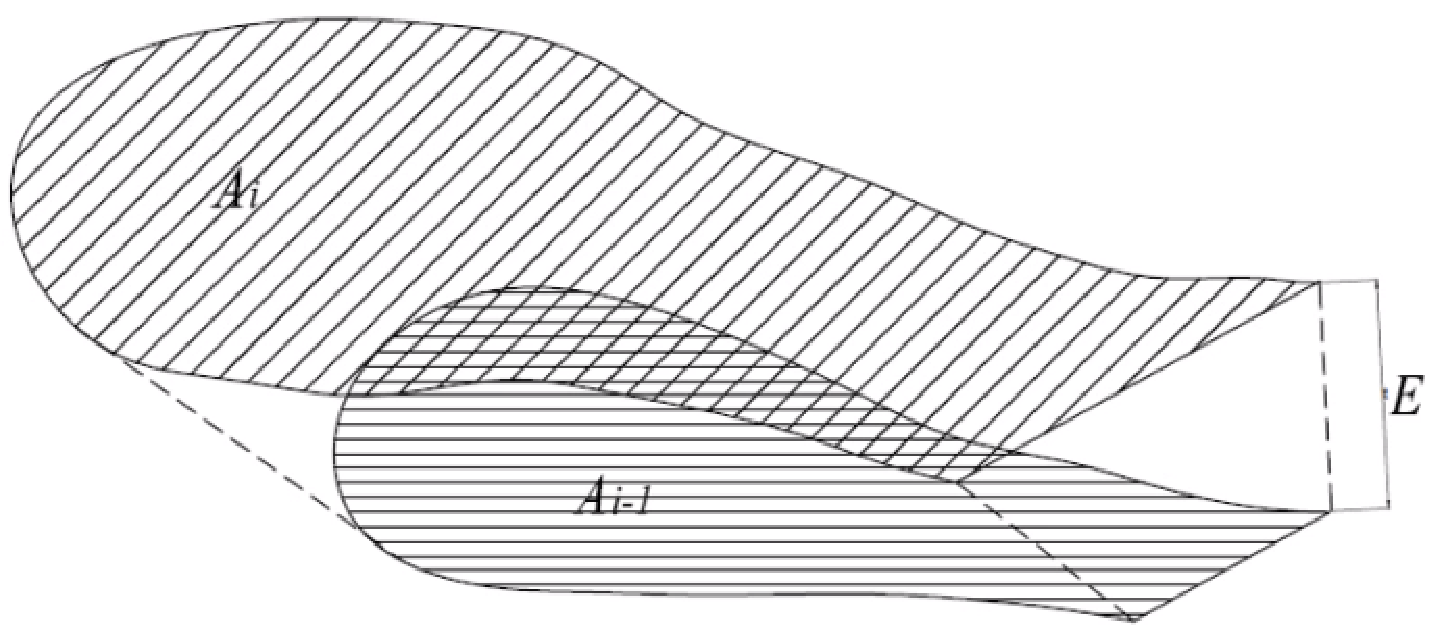
\includegraphics[width=0.5\textwidth]{ta44.pdf}
  \caption{Cálculo de volúmenes almacenados}
  \label{ta44}
\end{figure}

\begin{align}
    &\text{Tolerancia lineal }TL=1/5000\\
    &\text{Tolerancia angular }TA = 2a \sqrt{n}\\
    &\text{Tolerancia de nivelación }Tn =12.6 \sqrt{K} 
\end{align}

\begin{table}[h!]
    \centering\begin{tabular}{@{}ccc@{}}
    \toprule
    \begin{tabular}[c]{@{}c@{}}Tamaño del\\ vaso\end{tabular} & \begin{tabular}[c]{@{}c@{}}Escala del\\ plano\end{tabular} & \begin{tabular}[c]{@{}c@{}}Equidistancia\\ entre curvas\end{tabular} \\ \midrule
    Chico                                                     & 1:1000 a 1:2000                                            & 1.0                                                                  \\
    Mediano                                                   & 1:5000 a :10000                                            & 2.0                                                                  \\
    Grande                                                    & 1:10000 a 1:20000                                          & 5.0                                                                  \\ \bottomrule
    \end{tabular}
    \caption{Especificaciones para los planos}
    \label{tabta13}
    \end{table}

\subsection{Levantamiento de la cuenca de captación}

Una Cuenca de Captación es un área grande, limitada por un parteaguas, en la que debido a los desniveles topográficos, se originan partes altas y bajas que forman cauces, por los que se conducen todos los escurrimientos derivados del agua de precipitación ocurrida concurriendo todos éstos a en un ella, cauce común que los desaloja en una dirección determinada.

Este no es el concepto hidrológico

La Cuenca se determina a partir de la boquilla, por lo que deben definirse simultáneamente.

Determinar el área y otras características fisiográficas de la misma, para conocer los parámetros hidrológicos de Coeficiente de Escurrimiento, el Volumen de Escurrimiento Medio Anual y la Avenida Máxima Probable, necesarios para dimensionar la cortina y la obra de excedencias de la obra de almacenamiento por proyectar.

\subsubsection{Coeficiente de escurrimiento}

Es la relación que existe entre el volumen escurrido y el volumen precipitado
\begin{align*}
    Ce = \frac{Ve}{Vp}&& Ce = \frac{Ve}{Vp}\cdot 100
\end{align*}
Donde $Ce=$ Coeficiente de escurrimiento, $Ve$ el volumen escurrido en $m^3$ y $Vp$ es el volumen precipitado en $m^3$

Para estimar el $Ce$ en la práctica se recurre a tablas.

\begin{table}[h!]
    \centering\begin{tabular}{@{}ccc@{}}
    \toprule
    Factor                                                                                        & Condición                   & $Ce(\%)$ \\ \midrule
    \multirow{3}{*}{\begin{tabular}[c]{@{}c@{}}Cubierta\\ vegetal\end{tabular}}                   & Terrenos cultivados o pasto & 1-30     \\
                                                                                                  & Bosque                      & 5-20     \\
                                                                                                  & Sin cubierta vegetal        & 25-50    \\
    \multirow{4}{*}{\begin{tabular}[c]{@{}c@{}}Superficie de la\\ Cuenca ($km^2$)\end{tabular}}   & Hasta 10                   & 25       \\
                                                                                                  & Entre 10 y 100              & 15       \\
                                                                                                  & Entre 100 y 500             & 10       \\
                                                                                                  & Mayores de 500              & 5        \\
    \multirow{4}{*}{\begin{tabular}[c]{@{}c@{}}Precipitación\\ Media\\ Anual\\ (mm)\end{tabular}} & Hasta 800                   & 0-5      \\
                                                                                                  & Entre 800 y 1200            & 5-15     \\
                                                                                                  & Entre 1200 y 1500           & 15-35    \\
                                                                                                  & Más de 1500                 & 35-50    \\ \bottomrule
    \end{tabular}
    \caption{Definida por la secretaría de recursos hidráulicos (SRH)}
    \label{tabta14}
    \end{table}


    \begin{example}
        Supóngase que se desea determinar el valor del Coeficiente de Escurrimiento para una Cuenca cuya superficie es de 64.34 $km^2$, cubierto mayormente de bosque y con una precipitación media anual de 914 mm.
      \end{example}
      
      \begin{equation*}
        Ce =\frac{8.3 + 16.7}{2} =12.5\%
      \end{equation*}
      Por otra parte, en caso de que la Cuenca tenga fracciones de su superficie con cubierta vegetal diferente, deberá obtenerse un Ce medio ponderado, considerando como factor para la ponderación la proporción de superficie
      \begin{table}[h!]
        \centering\begin{tabular}{@{}ccc@{}}
        \toprule
        Concepto      & $Ce$ min & $Ce$ max \\ \midrule
        Bosque        & 5.00     & 20.00    \\
        Superficie    & 15.00    & 15.00    \\
        Precipitación & 5.00     & 15.00    \\
        Suma          & 25.00    & 50.00    \\
        Promedio      & 8.33     & 16.67    \\ \bottomrule
        \end{tabular}
        \caption{Ejemplo de cálculo de $Ce$}
        \label{tabta15}
        \end{table}
      \begin{equation*}
        Ce ce_1\cdot pA_1+Ce_2 + Ce_1\cdot pA_1 +\dots + Ce_n\dot pA_n
      \end{equation*}
      $pA_i$ es la porcentaje del área $A_i$
      
      \subsubsection{Norma de la SEMARNAT}
      
      Métodos para determinar el volumen medio anual de escurrimiento y describe el método para calcular el Ce, en función del tipo y uso del suelo y del volumen de precipitación anual de la cuenca en estudio
      
      Se clasifican los suelos de la cuenca, en 3 tipos: A suelos permeables, B suelos medianamente permeables, y C suelos casi impermeables, y al tomar en cuenta el uso actual del suelo, se obtiene el valor del parámetro Ke, con el que se calcula el Ce:
      \begin{table}[h!]
        \centering\begin{tabular}{@{}cc@{}}
        \toprule
        \begin{tabular}[c]{@{}c@{}}Tipo de\\ suelo\end{tabular} & Características                                                                                                                                                                                                    \\ \midrule
        A                                                       & \begin{tabular}[c]{@{}c@{}}Suelos permeables, tales como arenas \\ profundas y loess poco compactos.\end{tabular}                                                                                                  \\
        B                                                       & \begin{tabular}[c]{@{}c@{}}Suelos medianamente permeables, tales \\ como arenas de mediana profundidad: loess \\ algo más compactos que los correspondientes a los \\ suelos A; terrenos migajosos.\end{tabular} \\
        C                                                       & \begin{tabular}[c]{@{}c@{}}Suelos casi impermeables, tales como arenas \\ o loess muy delgados sobre una capa \\ impermeable, o bien arcillas.\end{tabular}                                                        \\ \bottomrule
        \end{tabular}
        \caption{Norma de la SEMARNAT}
        \label{tabta16}
        \end{table}
      \begin{align*}
        &Ke\leq 0.15&& Ke > 0.15\\
        &Ce =\frac{Ke\left(P_{ma} 205\right)}{2000}&&Ce =\frac{Ke\left(P_{ma} - 50\right)}{2000} +\frac{Ke - 0.15}{1.5}
      \end{align*}
      Ce se obtiene en decimal. Para \% debe multiplicarse por 100
      
      \begin{example}
        Una cuenca tiene 32\% de su área con pastizales en más el 75\% y en suelo tipo A, 46\% se superficie en suelo tipo B con bosque cubierto al 48\% restante 22\% en suelo tipo A ocupada y el con praderas permanentes. La magnitud de las precipitaciones se anota en el cuadro.
      \end{example}
      
      \begin{table}[h!]
        \centering\begin{tabular}{@{}cccccc@{}}
        \toprule
        \begin{tabular}[c]{@{}c@{}}\% de\\ superficie\end{tabular} & \begin{tabular}[c]{@{}c@{}}Tipo de\\ suelo\end{tabular} & Cubierta           & $Ke$ & \begin{tabular}[c]{@{}c@{}}$P_{ma}$\\ (mm)\end{tabular} & \begin{tabular}[c]{@{}c@{}}Ce\\ (\%)\end{tabular} \\ \midrule
        32                                                         & A                                                       & Pastizal poco      & 0.14 & 800                                                     & 7.7                                               \\
        45                                                         & B                                                       & Bosque 48\%        & 0.26 & 1200                                                    & 19.7                                              \\
        22                                                         & C                                                       & Pradera permanente & 0.30 & 950                                                     & 20.5                                              \\ \bottomrule
        \end{tabular}
        \caption{Datos del problema}
        \label{tabta17}
        \end{table}
      
      \begin{align*}
        Ce = 7.7\cdot 0.32 +19.7\cdot 0.46 + 0.5\cdot 0.22\\
        Ce =16.036\%
      \end{align*}
      \begin{table}[h!]
        \centering\begin{tabular}{@{}cccc@{}}
        \toprule
        \multirow{2}{*}{Uso de suelo}                   & \multicolumn{3}{c}{Tipo de suelo} \\
                                                        & A         & B         & C         \\ \midrule
        Barbecho, áreas sin cultivar y desnudas         & 0.26      & 0.28      & 0.30      \\
        \multicolumn{1}{l}{\textbf{Cultivos}}           &           &           &           \\
        Legumbres o rotación de cultivos                & 0.24      & 0.27      & 0.30      \\
        Granos pequeños                                 & 0.24      & 0.27      & 0.30      \\
        Pastizales \% de suelo cubierto                 &           &           &           \\
        Más de 75\% poco                                & 0.14      & 0.20      & 0.28      \\
        Del 50 al 75\% Regular                          & 0.20      & 0.24      & 0.30      \\
        Menos del 50\% Excesivo                         & 0.24      & 0.28      & 0.30      \\
        \multicolumn{1}{l}{\textbf{Bosque}}             &           &           &           \\
        Cubierto más de 75\%                            & 0.07      & 0.16      & 0.24      \\
        Del 50 al 75\%                                  & 0.12      & 0.22      & 0.26      \\
        Del 25 al 50\%                                  & 0.17      & 0.26      & 0.28      \\
        Cubierto menos del 25\%                         & 0.22      & 0.25      & 0.30      \\
        \multicolumn{1}{l}{\textbf{Zonas urbanas}}      & 0.26      & 0.29      & 0.32      \\
        \multicolumn{1}{l}{\textbf{Caminos}}            & 0.27      & 0.30      & 0.33      \\
        \multicolumn{1}{l}{\textbf{Pradera permanente}} & 0.18      & 0.24      & 0.30      \\ \bottomrule
        \end{tabular}
        \caption{Parámetros hidrológicos }
        \label{tabta18}
        \end{table}
      Se usa la fórmula del método racional
      \begin{equation}
        Q_{\max} = 0.278CeImAc
      \end{equation}
      Donde $Q_{max}$ Avenida máxima en $m^3/s$, $Ce$ Coeficiente de escurrimiento adimensional, $Im$ = Intensidad máxima de lluvia, en $mm/h$, $Ac$; Área de la Cuenca, en $km^2$; y 0.278: Coeficiente de conversión de unidades.
      
      $Im$, debe seleccionarse para el período de retorno (15, 25. 50 o 100 años, por ejemplo) y que corresponda al llamado tiempo de concentración Te que se obtiene de la fórmula de Kirpich
      \begin{equation}
        Tc =0.00325\frac{Lc^{0.77}}{Sc^{0.385}}
      \end{equation}
      $Le$ y $Se$ son la longitud y la pendiente del Cauce Principal de la Cuenca, se entra a la gráfica con el $Te$ y $se$ obtiene Im
      
      Supóngase $Im$ de 85mm/h para calcular el $Q_{max}$ para la cuenca:
      \begin{align*}
        Q_{\max } = 0.278\cdot 0.16\cdot 85\cdot 853\\
        Q_{\max } = 3225.022 \frac{m^2}{s}
      \end{align*}
      Con el estudio topográfico se determina $Ac$, Lc$, Sc$ y las fracciones de cuenca con distintas coberturas.
      \begin{figure}[h!]
      \centering
        \includegraphics[width=0.5\textwidth]{ta45.pdf}
        \caption{Avenida máxima probable (Qmax)}
        \label{ta45}
      \end{figure}
      
      Las cuencas grandes y medianas se identifican y determinan sus características en cartas topográficas o con imágenes de satélite mediante sistemas de información geográfica
      
      Sólo las cuencas pequeñas se levantan topográficamente
      
      \begin{enumerate}
        \item Se hace un recorrido de campo localizando el parteaguas
        \item  Se establecen PCA mediante una Poligonal Cerrada con LCA lo más largas posible compensando las áreas externas que son e internas que no son.
        \item Se levanta la Poligonal midiendo con teodolito y estadal y por estadia, con teodolito y MED, con estación total o con equipos PGS.
      \end{enumerate}
      Dada la baja precisión requerida se pueden emplear los Métodos de Estaciones Alternas midiendo los Rumbos o Azimut de las LCA y el Método de Intersecciones para puntos alejados o inaccesibles, de manera combinada o independiente.

      Con el trabajo de gabinete, se debe determinar el Área de la Cuenca y los valores de los parámetros hidrológicos indicados, para lo cual se debe comprobar y compensar previamente la Poligonal Cerrada y calcular las coordenadas de sus vértices.

      Se elabora un plano con las siguientes definiciones
      \begin{table}[h!]
          \begin{tabular}{@{}ccc@{}}
          \toprule
          \begin{tabular}[c]{@{}c@{}}Tamaño de\\ la cuenca\end{tabular} & \begin{tabular}[c]{@{}c@{}}Escala del \\ plano\end{tabular} & \begin{tabular}[c]{@{}c@{}}Equidistancia\\ entre curvas\end{tabular} \\ \midrule
          Chico                                                         & 1:5000                                                      & 5.0                                                                  \\
          Mediana                                                       & 1:10000                                                     & 10.0                                                                 \\
          Grande                                                        & 1:100000                                                    & 10.0 a 20.0                                                          \\ \bottomrule
          \end{tabular}
          \caption{Trabajo de gabinete}
          \label{tabta19}
          \end{table}
      
      Precisiones y tolerancias
      \begin{align}
          &Tl = \frac{1}{100}\to \frac{1}{500}\text{ Tolerancia angular}\\
          &Ta = 3a \sqrt{n}\to 2a \sqrt{n}\text{ Tolerancia angular}
      \end{align}
      
      Obtener una serie de datos topográficos e hidrológicos que permitan determinar el Gasto Máximo o Avenida Máxima Probable del cauce, que se emplea para el diseño de la obra de excedencias de las presas de almacenamiento de agua.
      El área A y el perímetro mojado P se mide o calcula del dibujo de la sección hidráulica resultado del levantamiento.
      La velocidad se calcula con la fórmula de Manning
      El gasto se obtiene de la ecuación de continuidad.
      
      A: se mide en el dibujo
      \begin{align}
          &v = \frac{1}{n}r^{\frac{2}{3}}s^{\frac{1}{2}}\\
          &r = \frac{A}{P}\land Q = A\cdot v\\
          &Q_{\max} =\frac{A^{\frac{5}{3}}S^{\frac{1}{2}}}{nP^{\frac{2}{3}}}
      \end{align}
      
      $Q$ avenida máxima en $m^3/s$, $v$ velocidad medidas del agua en $m/s$, $n$ coeficiente de rugosidad de Manning en $m^{-1/3}/s$m $r$ Radio hidráulico, $A$ Área hidráulica de la sección transversal en $m^2$, $P$ perímetro mojado de la sección transversal en $m$ y $s_0$ pendiente longitudinal del fondo del cauce adimensional.
      \begin{table}[h!]
          \begin{tabular}{@{}cc@{}}
          \toprule
          \multirow{2}{*}{Condición del cauce}                  & n             \\ \cmidrule(l){2-2} 
                                                                & $(m^{1/3}/2)$ \\ \cmidrule(r){1-1}
          Limpio, recto y sin pozos a nivel máximo              & 0.029         \\
          Como el anterior, con vegetación y piedras            & 0.035         \\
          Sinuoso, limpio con pozos y rápidos                   & 0.039         \\
          Como el anterior a niveles bajos                      & 0.042         \\
          Sinuoso, pozos y rápidos con vegetación y piedras     & 0.047         \\
          Como el anterior, a niveles bajos y con grandes rocas & 0.052         \\
          Pantanoso con vegetación y pozos profundos            & 0.065         \\
          Muy pantanoso y con mucha vegetación                  & 0.112         \\ \bottomrule
          \end{tabular}
          \caption{Tabla de Linsley, Kohler y Paulus (1975)}
          \label{tabta20}
          \end{table}
      
      Las condiciones que debe reunir el tramo de cauce:
      \begin{enumerate}
          \item Que sea lo más recto posible y uniforme tanto en su sección como en su pendiente. Estas condiciones son en extremo importantes ya que en la medida que no se cumplan, el régimen hidráulico es menos establecido y, por lo tanto, la ecuación de Manning no es válida para el cálculo de la velocidad del flujo.
          \item Una longitud de entre 100 y 400 m. Se recomienda como longitud óptima 200 m; aunque si ello no es posible, se debe procurar que cuando menos sea igual a seis veces el ancho.
          \item Las márgenes deben ser altas y que sobrepasen las huellas máximas, para garantizar que no haya desbordamientos en consecuencia, salidas o entradas al cauce que modifiquen el valor de la Avenida Máxima a determinar.
          \item No debe haber vegetación alta. Aunque este aspecto se puede considerar en la determinación del coeficiente de Manning, lo más conveniente es que el tramo elegido tenga la menor vegetación posible.
      \end{enumerate}
      
      \subsubsection{Levantamiento por el MT de secciones transversales}
      
      \begin{enumerate}
          \item Se establece una LCA con dos o tres PCA como Poligonal Abierta con tránsito o teodolito y cinta (o con teodolito y distanciómetro o estación total), por uno de los márgenes del cauce y más o menos paralela a su eje y por arriba del nivel de aguas máximas, o en su fondo si no hay agua.
          \item Sobre la LCA trazada, se ubican estacas cada 20 m o a otra equidistancia conveniente, de manera que se tenga el mayor número posible de secciones. La Elevación o Z de estos puntos se determina con nivel montado por Nivelación de Perfil. Por supuesto que si el trazo se hace con distanciómetro o estación total se obtendrán directamente coordenadas relativas o absolutas, respectivamente, para cada uno de los estos puntos.
          \item El trazo y levantamiento de las Secciones Transversales, se hace registrando en cada una, todos los cambios de pendiente que permitan dibujarlas en gabinete lo más fiel posible; en particular, se debe registrar la ubicación de las huellas máximas del flujo, en ambas márgenes de preferencia, así como el fondo del cauce.
      \end{enumerate}
      
      El trabajo se puede hacer de manera simultánea midiendo con cinta y nivelando con nivel montado y, más aún, cuando se hace con distanciómetro o estación total.
      Al momento de hacer el levantamiento, se debe tomar nota de todos las condiciones del cauce que permitan en gabinete, definir lo más acorde posible el valor del coeficiente de rugosidad
      
\section{Estudios Topográficos para Zonas de Riego}
      
      La actividad agrícola en México, se realiza en cuatro grandes condiciones con características y circunstancias
      socioeconómicas,
      agroambientales y de
      organización para la producción, peculiares diferentes, que son los:
      \begin{itemize}
          \item Distritos de Riego,
          \item Unidades de Riego,Distritos de Temporal Tecnificado, y
          \item Arcas de Temporal.
      \end{itemize}
      Los Distritos de Riego (DR), son grandes extensiones de tierra del orden de decenas o incluso centenas de miles de hectáreas con buenas características agronómicas para la producción agrícola, que cuentan con infraestructura hidroagrícola, conformada por obras de almacenamiento o para el aprovechamiento del agua para riego, sistemas de conducción, distribución y aplicación a los cultivos, construida mayormente por entidades gubernamentales, que les confieren una alta productividad y que benefician a los usuarios de ellas, con buenos rendimientos y utilidades.
      
      85 DR con 3.5 millones de ha
      
      Las Unidades de Riego (UR), son zonas agrícolas con superficies del orden de entre 50 y 250 hectáreas, con buenas tierras para la producción agrícola y que suman alrededor de 50,000; cuentan con fuentes de agua para riego e infraestructura para su aprovechamiento, conducción, distribución y aplicación de los cultivos, construida, conservada y operada por los propios usuarios, con muy poca participación gubernamental y que representan un 55\% de la superficie bajo riego del país con alrededor de 4.0 millones de hectáreas.
      
      Los Distritos de Temporal Tecnificado (DTT), que suman 26, son zonas de producción agrícola con superficies promedio de 70 mil ha para un total de 1.82 millones de hectáreas, que se localizan en las regiones de país, donde los excesos de agua de lluvia se constituyen en un problema y, por tanto, se ha construido con recursos gubernamentales, infraestructura para su desalojo, a fin de evitar o reducir los daños y asegurar la cosechas de los cultivos que en ellas se establecen.
      
      Las Zonas Agrícolas de Temporal (ZAT) son aquellas que no cuentan con infraestructura para el aprovechamiento del agua para riego, ni están organizadas, de modo que los apoyos gubernamentales son prácticamente nulos, y son propiedad de productores individuales con superficies unitarias que van desde menos de una ha hasta algunas decenas de ellas, con tierras de baja productividad y que se distribuyen en todo el país, por todo lo cual son de poca importancia productiva y económica.
      
      Siendo pequeñas, pueden levantarse empleando los Procedimientos de Poligonales y Nivelación Diferencial para el establecimiento del SPLCA y si son de varios cientos de ha, pueden emplearse cualquiera de los PTP de Triangulación o Trilateración para el establecimiento el SPLCA; y, en ambos casos, el Método de Radiaciones para el levantamiento de PCD.
      
      El levantamiento de terrenos que constituyen o constituirán una zona de riego, puede llevarse a cabo utilizando diversos Procedimientos Topográficos para el establecimiento de Puntos y Líneas de Control y Apoyo tanto en planimetría como en elevación, así como varios instrumentos y Métodos Topográficos para el levantamiento de Puntos para Configuración y/o de Detalle.
      
      Estos levantamientos, invariablemente se deberán ligar el Sistema de Puntos y Líneas de Control y Apoyo empleados para los estudios topográficos para el proyecto y construcción de las fuentes de abastecimiento del agua para riego, en particular cuando se trata de una obra de almacenamiento
      
      Siendo los DR las zonas agrícolas de mayor importancia por su magnitud y productividad, son a los que se da mayor atención para su estudio topográfico, y su tratamiento se diferencia en primera instancia, según ya exista la zona de riego o vaya a ser de nueva creación, y luego considerar los instrumentos o equipos disponibles, separando también el establecimiento del SPLCA en planimetría y en altimetría y luego para el levantamiento de PCD, y aun del caso en que se pueda hacer todo el trabajo simultáneamente aplicando Procedimientos y Métodos
      
      Topográficos Tridimensionales y empleando los instrumentos y equipos que lo hacen posible.
      
      \subsection{Cuadrícula rectangular}
      
El Procedimiento Topográfico Planimétrico de Cuadrícula Rectangular, consiste, de una serie de LCA perpendiculares y orientadas en las direcciones NS y EW, espaciadas a iguales distancias en ambas direcciones, que se trazan con tránsito o teodolito y cinta de acero o distanciómetro y cuyas intersecciones, constituyen los PCA que se definen con monumentos de concreto, mismos que son nivelados con nivel montado para conocer su elevación
\begin{figure}[h!]
\centering
  \includegraphics[width=0.5\textwidth]{ta46.pdf}
  \caption{Descripción y aplicabilidad}
  \label{ta46}
\end{figure}
Se emplea principalmente para el levantamiento de grandes extensiones planas de terreno que se aperturarán a la agricultura bajo riego, por lo que se definirá el parcelamiento y se proyectará y construirá la infraestructura hidroagrícola, consistente en los sistemas de conducción y distribución del agua, las redes de drenaje, los caminos y las estructuras de almacenamiento, control operación, cruce y conservación.

\begin{itemize}
    \item Se ubica aproximadamente al centro del terreno
    \item Que el sitio esté despejado y sea de fácil localización y acceso
    \item De modo que se facilite el trazo del Meridiano Principal y del Paralelo Base.
    \item Se define con un Monumento mayor
\end{itemize}
\begin{figure}[h!]
\centering
  \includegraphics[width=0.5\textwidth]{ta47.pdf}
  \caption{Monumento mayor para vértices de cuadros principales}
  \label{ta47}
\end{figure}

Para trazar el sistema coordenado principal:
\begin{itemize}
    \item Se determinan con precisión las Coordenadas UTM del origen y de otro sobresaliente cualquiera.
    \item Se determina el azimut de la LCA así definida.
    \item Se mide el valor del azimut en sentido antihorario, con lo que se define el sentido norte N, sobre la que se traza el MP colocando un punto en la dirección definida
\end{itemize}

\begin{figure}[h!]
\centering
  \includegraphics[width=0.5\textwidth]{ta48.pdf}
  \caption{Orientación del sistema}
  \label{ta48}
\end{figure}

En el establecimiento del MP se realizan estos pasos:
\begin{enumerate}
    \item Se estaciona el Teodolito en el punto 1 sobre la dirección definida para el MP y se visa el punto Origen en posición directa del telescopio.
    \item Se da vuelta de campana al telescopio y se ubica y define con trompo y tachuela el punto 2a a una distancia aproximadamente mayor de 500 m, con lo que el telescopio queda en posición inversa.
    \item Se gira el telescopio sobre su eje vertical $180^{\circ}$, de manera que se visa el punto Origen en posición inversa del telescopio.
    \item Se da vuelta de campana al telescopio, ubicando y definiendo con trompo y tachuela el punto 2b a la misma distancia que el punto 2a, quedando ahora el telescopio en posición directa. Teóricamente, la ubicación de los puntos 2a y 2b, debe ser la misma; sin embargo, sería una casualidad que esto ocurriera, pues siempre habrá errores accidentales asociados con la operación y el desajuste del instrumento.
    \item Se mide con una cinta metálica la distancia que separa los puntos 2a y 2b y se ubica el punto 2, a la mitad de dicha medida, definiéndolo con un trompo y una tachuela.
    \item Se repite todo el proceso iniciando en posición inversa del telescopio al visar el origen.
\end{enumerate}
\begin{figure}[h!]
\centering
  \includegraphics[width=0.5\textwidth]{ta49.pdf}
  \caption{Medición}
  \label{ta49}
\end{figure}

%Para la medición lineal, el error lineal EL y la tolerancia lineal TL se calculan como sigue:
%\begin{align}
%    EL = DHi DHd\\
%    TL = \pm 
%\end{align}

Haciendo estación en el Origen con un teodolito de precisión se mide un ángulo de $90^{\circ}$ en sentido horario a partir del MP. La dirección resultante corresponde al Este, y por lo tanto al PB.

Se coloca un trompo para establecer la dirección determinada.

En dicha dirección se hace el trazo del PB idénticamente que como se describió para el MP

Todo el procedimiento se repite para el trazo del MP hacia el sur y del PB hacia el Oeste

Si no se cuenta con un teodolito de precisión se establece un ángulo de 90 y luego se mide por repeticiones y se calcula y corrige el error lineal generado

\begin{figure}[h!]
\centering
  \includegraphics[width=0.5\textwidth]{ta50.pdf}
  \caption{Trazo del PB}
  \label{ta50}
\end{figure}
En el cuarto vértice se verifica el cierre. Si los trazos lineales no coinciden, la distancia entre los puntos finales es el error lineal EL que se debe comparar con la TL.

Los cuadros principales se forman con el trazo de los llamados paralelos y meridianos, que son líneas perpendiculares respectivamente al MP y al PB en puntos múltiplos de 5 km sobre cada uno de éstos, de modo que los cuadros resultan de 5 km de lado. Esto implica medir ángulos precisos de $90^{\circ}$ en los dos puntos de inicio del paralelo y del meridiano respectivo.

El trazo del meridiano y del paralelo se hace igual que se hizo el del MP y del PB.
\begin{figure}[h!]
\centering
  \includegraphics[width=0.5\textwidth]{ta51.pdf}
  \caption{Trazo de cuadros principales}
  \label{ta51}
\end{figure}
Se mide el ángulo cuya diferencia con $90^{\circ}$ es el error angular $EA$, las tolerancias son: $TA= \sqrt{10^2N+5^2n}$, donde $N$ son vértices ortogonales, $n$ puntos donde se prolongó alineamiento (40) y $TA$ 47.417 segundos. TL=40cm. Si se cumplen las tolerancias, se definen como correctos los puntos de intersección.
Se hace trazando los Meridianos Secundarios. Pueden presentarse DOS POSIBILIDADES

Si se observa el punto final, se genera solo error lineal que no debe ser mayor de 10 cm. El error se distribuye entre los puntos intermedios proporcionalmente a las distancias medidas hasta ellos, en la dirección del trazo.
\begin{figure}[h!]
\centering
  \includegraphics[width=0.5\textwidth]{ta52.pdf}
  \caption{Trazo de cuadros secundarios}
  \label{ta52}
\end{figure}
Si no se observa el punto final, se genera un ERROR LINEAL y un ERROR ANGULAR. Las correcciones se hacen linealmente en las direcciones x y y proporcionalmente las distancias recorridas en ambas direcciones.
\begin{figure}[h!]
\centering
  \includegraphics[width=0.5\textwidth]{ta53.pdf}
  \caption{Sustitución de un trompo por un monumento}
  \label{ta53}
\end{figure}

\subsubsection{Triangulación para el SPLCA}

En el PTP de Triangulación el establecimiento de los Puntos y Líneas de Control y Apoyo, se hace cubriendo el terreno a levantar, con un sistema de triángulos, en los que se miden todos los ángulos generados y en cambio, un número limitado (uno, dos o tres), lados que se denominan Bases, mismos que también se orientan; las longitudes de los lados restantes se calculan trigonometricamente en cada triángulo aplicando la Ley de Senos, para finalmente determinar las posiciones de los puntos y las direcciones de la líneas.

Se aplica al levantamiento de grandes áreas en producción o explotación en las que está definido el parcelamiento, las vías de comunicación y la infraestructura de operación y se requiere conocer sus características o proyector y construir infraestructura adicional para mejorar condiciones productivas
Los valores finales

promedios de las 4 observaciones

La suma se los valores finales debe se exactamente $360^{\circ}$

Los ángulos se miden en cada vértice, en sentido horario e iniciando en el vértice más conveniente

En cada vértice los ángulos se miden con 4 repeticiones iniciando en los valores 000$^{\circ}$ 00$^{\prime}$00$^{\prime\prime}$, 045$^{\circ}$ 02$^{\prime}$ 30$^{\prime\prime}$, 090$^{\circ}$ 05$^{\prime}$ 00 y 135$^{\circ}$ 07$^{\prime}$ 30$^{\prime\prime}$.

Las mediciones se hacen con un instrumento de precisión al segundo.

La denominación de los ángulos con letras es particular para un PVC de 5 triángulos y no puede generalizarse. Para una generalización se usa la nomenclatura binomial,

La nomenclatura binomial consiste en que a cada ángulo se le asignan dos subíndices denominados:

$i:$ que se refiere al número de triángulo, que se

enumeran de 1 an iniciando en cualquiera y en el sentido de las manecillas del reloj.

$j:$ que denomina a los ángulos dentro de cada triángulo, por lo que varía de 1 a 3 iniciando del vértice central y numerados en sentido horario

Así el ángulo A51 es del triángulo 5 y del vértice central.

\begin{figure}[h!]
\centering
  \includegraphics[width=0.5\textwidth]{ta54.pdf}
  \caption{La misma nomenclatura se usa para las correcciones $C$}
  \label{ta54}
\end{figure}

Las condiciones de cierre en nomenclatura binomial en cada triángulo:
\begin{equation}
    \sum_{j = 1}^3 A_{ij} +\sum_{j =1}^3 C_{ij} = 180^{\circ}
\end{equation}
En el vértice central:
\begin{equation}
    \sum_{j = 1}^3 A_{i1} +\sum_{i=1}^3 C_{i1} = 360^{\circ}
\end{equation}
La condición lineal:
\begin{equation}
\sum_{i = 1}^n \log{\left(\sin{(A_{i2})}\right)} =\sum_{i = 1}^n \log{\left(\sin{(A_{i3})}\right)}
\end{equation}
La teoría de mínimos cuadrados indica que la suma de las correcciones $C_{ij}$ al cuadrado debe ser un mínimo:
\begin{equation}
    U(C_i^2)\implies \frac{\delta U(C_i^2)}{U(C_i^2)}
\end{equation}
Haciendo un ajuste a la condición lineal:
\begin{equation*}
    \sum_{i = 1}^n \log{\left(\sin{(A_{i2}) + C_{i2}}\right)} =\sum_{i = 1}^n \log{\left(\sin{(A_{i3}) + C_{i3}}\right)}
\end{equation*}
Llegando a ésta última expresión:
\begin{equation}
    \log{\sin{\left(A_{ij} + C_{ij}\right)}} = \log{\sin{\left(A_{ij}\right)}} + \left[\log{\sin{A_{ij} + \frac{1}{3600}}} - \log{\sin{A_{ij}}} \right] C_{ij} \times 10^6
\end{equation}
\subsection{Nivelación de los PCA}
Independientemente de cuál de los Procedimientos Topográficos de Planimetría se emplee para el establecimiento en planta de los Puntos de Control y Apoyo, la determinación de su Coordenada Zo Cota, invariablemente se hace por el Procedimiento Topográfico Altimétrico de Nivelación Diferencial
\begin{figure}[h!]
\centering
  \includegraphics[width=0.5\textwidth]{ta55.pdf}
  \caption{Cuando se establecen por cuadrícula}
  \label{ta55}
\end{figure}
La nivelación de los PCA de una Cuadrícula Rectangular, se inicia con el Cuadro Principal N5,E5 aplicando el PTA de Nivelación Diferencial entre cada par consecutivo de PCA (estableciendo Puntos de Liga cuando y donde se requieran), iniciando por el PCA del Origen, siguiendo el sentido horario para recorrer todo el perímetro y regresando al Origen para la comprobación.
\begin{figure}[h!]
\centering
  \includegraphics[width=0.5\textwidth]{ta56.pdf}
  \caption{Nivelación de cuadrados principales}
  \label{ta56}
\end{figure}
\subsubsection{Nivelación de circuitos simultáneos y su compensación por mínimos cuadrados}
La teoría de mínimos cuadrados establece que los valores más probables de los errores accidentales que ocurren en cualquier tipo de mediciones, son aquellos que hacen mínima la suma de sus cuadrados, por lo cual, partiendo del supuesto de que en un trabajo de nivelación dado, se han eliminado los errores sistemáticos y las equivocaciones o errores gruesos, esta teoría puede aplicarse para el cálculo de las correcciones que se le deben asignar a los Desniveles.

La metodología es aplicable a la compensación simultánea de Circuitos Cerrados analíticamente; la distribución del Error de Nivelación E, se hace con base en la condición que impone la teoría de mínimos cuadrados. e involucrando una ponderación que puede calcularse proporcional a las distancias horizontales DH o a los desniveles PE entre los PCA consecutivos sobre los Circuitos de Nivelación. Cuando los PCA que conforman el circuito se establecen mediante Poligonales. Triangulación o Trilateración, puede emplearse cualquiera de los criterios para el cálculo del Factor de Ponderación Fp. dado que tanto las distancias como los desniveles resultan heterogéneos; mientras que, en el caso en que los PCA sean establecidos por Cuadrícula Rectangular (tanto en los Cuadros Principales como en los Secundarios), se deben emplear los desniveles para el cálculo de dicho factor, debido a que las distancias entre PCA resultan muy similares y no sería, por ello, conveniente su empleo. Evidentemente, cuando se emplean las distancias para el cálculo del Factor de Ponderación. Esta ha de ser la correspondiente al recorrido de nivelación, misma que puede determinarse con la fórmula de Estadia simple, si se hace el trabajo de nivelación en campo por el Método de los Tres Hilos.
\begin{figure}[h!]
\centering
  \includegraphics[width=0.5\textwidth]{ta57.pdf}
  \caption{nivelación de circuitos}
  \label{ta57}
\end{figure}
\begin{equation}
    Fp_k =\frac{\frac{1}{m}\sum_{k = 1}^m\,DH_k}{DH_k}
\end{equation}
Partiendo del PCA de Z conocida o del BN de partida para cada circuito, el error de nivelación para el -ésimo circuito Pz, se calcula con la expresión siguiente, en la que mi, es el número de tramos involucrados en el circuito i y Pz, es el desnivel correspondiente al j-ésimo tramo del circuito i..
%%%%%%%%%%%%%%%%%%%
Por lo anterior, es necesario además asignar lo que denominaremos como Signo de Circuito (S) a cada tramo en todos los circuitos, con base en la siguiente convención: partiendo del PCA de Z conocida y de partida o del BN en cada circuito, y siguiendo el sentido horario, se asigna signo positivo a los tramos en que éste coincida con el sentido del circuito de nivelación y signo negativo a los tramos en que ello no ocurra. Denotando por C a la corrección correspondiente al desnivel del j-ésimo tramo del circuito i, se establece para cada circuito una ecuación de condición de la forma de la 4.68:
\begin{equation}
    Ez_i =\sum_{j = 1}^m\,Cz_{ij}= 0
\end{equation}
El signo aquí considerado para las correcciones C. debe ser el Signo de Circuito correspondiente. Es evidente que el número de ecuaciones de condición del tipo 4.68. es igual al número de circuitos de nivelación en el sistema.

Por otra parte, de la teoría de mínimos cuadrados, se tiene que la suma de los cuadrados de los errores E debe ser un mínimo: lo que matemáticamente y en términos de las correcciones Cz, se expresa por la ecuación 4.69, en la cual se denota a las correcciones C con el subíndice k, pues corresponden a las que se definen para cada tramo, independientemente del circuito al que pertenezcan.

\begin{equation}
    \sum_{k = 1}^m\,\left( - Cz_k\right)^2 = minimo
\end{equation}

De lo expresado en los párrafos precedentes, es claro que se tienen n 1 ecuaciones para un total de incógnitas C, por lo que en principio el sistema es insoluble: sin embargo, debido a que en realidad, se tiene un problema de optimización de la función 4.69 sujeta a las restricciones impuestas por las ecuaciones de condición del tipo 4.68, tal situación se puede resolver aplicando la Técnica de Multiplicadores de Lagrange, la cual permite transformar un problema de máximos y mínimos con restricciones, a otro de máximos y mínimos libres (sin restricciones), correlacionando variables originales con otras variables intermedias (que son precisamente los Multiplicadores de Lagrange). para finalmente obtener un sistema de igual número de ecuaciones normales que de incógnitas (los multiplicadores de Lagrange), que puede resolverse por cualquier método conocido.

Esta técnica aplicada al problema que se discute, consiste en los siguientes pasos:
\begin{itemize}
    \item Cada una de las $n$ ecuaciones de condición, se multiplica por un multiplicador de lagrange $\lambda_i$ con lo que se obtienen $n$ ecuaciones:
    \begin{equation}
        a
    \end{equation}
    \item a
    \item Se obtiene la función $U\left\langle Fp_k,\lambda_k,Cz_k \right\rangle $ a minimizar formada por la suma de la función $F\left\langle \right\rangle $
    \item a
    \item Sustituyendo las ecuaciones de correlación 4.73, en las ecuaciones de condición originales 4.68, resulta un sistema de n ecuaciones normales de primer grado con n incógnitas que son los m multiplicadores de Lagrange A, cuya solución arroja sus valores.
    \item De la sustitución de los valores de los 2 en las ecuaciones de correlación correspondientes, se obtienen los valores de las correcciones $Cz_k$.
    \item Los valores de las correcciones asociadas a cada circuito (Cz) difieren solamente en signo respecto a la C correspondiente y se obtiene de multiplicar la Czz y el Signo de Circuito (S) respectivo, asignado al principio del trabajo de compensación; lo cual se expresa matemáticamente por la expresión 4.74:
    \begin{equation}
        Cz_{ij} = S_{ij} \times Cz_k
    \end{equation}
    Debe ser claro que el número de correcciones $Czy$ será mayor al número de correcciones Cze en el número de tramos comunes en el sistema; más aún, $Cz_{ij} Cz_k$ y $Cz_{i+1}=-Cz_k$. para los tramos comunes si los circuitos $i$ e $i+1$ son contiguos.
    \item Por supuesto, los desniveles compensados en cada circuito $PCz_{ij}$, resultan de la suma de desnivel observado ($Pz_{ij}$) y la corrección correspondiente $Cz_i$, como lo expresa la expresión 4.75.
\end{itemize}
%%%%%%%%%%%%%%%%%%%%%%%%%%%%%%%%%
%%%%%%%%%%%%%%%%%%%%%%%%%%%%%%%%%
%%%%%%%%%%%%%%%%%%%%%%%%%%%%%%%%%
%%%%%%%%%%%%%%%%%%%%%%%%%%%%%%%%%
%%%%%%%%%%%%%%%%%%%%%%%%%%%%%%%%%
%%%%%%%%%%%%%%%%%%%%%%%%%%%%%%%%%
%%%%%%%%%%%%%%%%%%%%%%%%%%%%%%%%%
%%%%%%%%%%%%%%%%%%%%%%%%%%%%%%%%%
%%%%%%%%%%%%%%%%%%%%%%%%%%%%%%%%%
%%%%%%%%%%%%%%%%%%%%%%%%%%%%%%%%%
%%%%%%%%%%%%%%%%%%%%%%%%%%%%%%%%%
\section{Localización y trazo de canales}

Una canal se define, desde el punto de vista hidráulico, como el conducto de sección geométrica abierta o cerrada que conduce agua por efecto principal de la fuerza de gravedad y que, por tanto, presenta en su fondo una pendiente longitudinal descendente, pequeña y uniforme, que se denota por $S_o$ y una superficie libre del agua ($SLA$) con una pendiente SA prácticamente de igual magnitud. Si bien pueden tener distintas formas geométricas, las secciones hidráulicas más comunes son la rectangular, la parabólica (a la que se pueden aproximar las secciones naturales o sin revestir) y la trapecial, siendo esta última la de uso más frecuente, independientemente de que pudiera ser alojada en tierra o estar revestida con concreto, mampostería u otros materiales. La figura 5.1 muestra un esquema de la sección hidráulica transversal al flujo del agua y una longitudinal (en el sentido del flujo) de un canal de forma trapecial, en la que se muestran sus elementos geométricos e hidráulicos; a saber: Ancho de la plantilla ($b$), Tirante ($v$). Talud o inclinación de la pared con respecto a la vertical ($m$), Ancho de la superficie libre del agua, Ancho de la corona ($C$), Área hidráulica, Perímetro mojado ($P$), y Pendiente longitudinal del fondo o de la rasante ($S_a$). El Área Hidráulica 4 en $m^2$, se obtiene de la expresión 5.1 y el Perímetro Mojado P en m con la 5.2, si se introduce en ellas el Ancho de la plantilla $b$ en $m$, el Tirante $y$ en $m$, y el Talud m en decimal.

\begin{align}
    &A = by_6my^2\\
    &P = b + 2y \sqrt{m^2+ 1}
\end{align}

Respecto a su uso o aplicación, los canales se emplean para conducir agua de un punto a otro, en los casos en que el flujo va de una cota alta a una inferior, cuando el ingreso de contaminantes no es tan importante y cuando no se requiere presión en la descarga, pues esta equivale a la presión atmosférica. La conducción del agua en canales presenta pérdidas por infiltración y por evaporación, lo que, independientemente del material de sus paredes, de su longitud y de su condición abierta o cerrada, implica grandes pérdidas, y como consecuencia, baja eficiencia, por lo que su aplicación también está condicionada a esta circunstancia; es decir, se emplean cuando las pérdidas de gasto y energía o presión no son relevantes porque la disponibilidad sea mayor que el requerimiento. A pesar de lo anterior, la aplicación fundamental de los canales en México

\begin{figure}[h!]
\centering
  \includegraphics[width=0.5\textwidth]{ta58.pdf}
  \caption{Sección transversal y longitudinal de un canal de forma trapecial mostrando sus }
  \label{ta58}
\end{figure}

Por las consideraciones y estudios que se deben realizar para su localización y trazo, los canales se pueden considerar como Vías de Comunicación, que se definen en general, como el espacio, medio o conducto proyectado, construido y operado por el hombre, que sirven para llevar o transportar personas, vehículos (terrestres, marítimos o aéreos), fluidos (agua, combustibles, energía eléctrica), señales de comunicación, etc., de un lugar a otro. La definición en este sentido tan amplio, permite incluir a todos los tipos de vías de comunicación terrestres, fluviales, marítimas y aéreas: es decir que incluye caminos, carreteras, autopistas, vías férreas, canales, tuberías, drenajes, líneas de transmisión eléctrica, de telefonía, de internet, de televisión por cable, rutas marítimas y aéreas, entre otras.

Las Vías de Comunicación terrestres pueden agruparse en los siguientes dos tipos:
\begin{enumerate}
    \item Aquellas cuyo trazo no es afectado por la topografía del terreno, porque no están condicionadas a un valor determinado ni al sentido de la pendiente, como es el caso
    de las líneas de transmisión eléctrica, de telefonía, de señales de internet, así como las tuberías que conducen agua u otros fluidos a presión.
    \item Aquellas en cuyo trazo y construcción se debe considerar un valor determinado de pendiente, como por ejemplo los caminos carreteros, cuyas pendientes máximas deben estar entre $\pm$3 y $\pm$10\%, según su importancia; las vías de ferrocarril, cuyas pendientes máximas deben oscilar entre $\pm$2 y $\pm$ 3\%), y los canales, cuyas pendientes debe ser muy pequeñas (en general menores de $\pm$0.1\%), y siempre negativas.
\end{enumerate}

De otra parte, la situación ideal en el trazo de toda la vía de comunicación es que sea recto
desde su origen hasta su punto final y a nivel, pero, al presentarse los accidentes topográficos del terreno y otros obstáculos, así como la, la condición de pasar por puntos obligados, se hace necesario buscar los lugares más fáciles y convenientes para salvarlos, y en forma económica, lo que implica que se tengan que incluir curvas tanto horizontales como verticales que unen tramos rectos de distinta dirección y longitud.

\begin{enumerate}
    \item Línea de conducción o canal principal.
    \begin{enumerate}
        \item Canal muerto, inicia en la fuente de abastecimiento y termina en el inicio de la zona de riego; de ordinario se construye en excavación: la otra parte
        \item Tramo sobre la zona de riego, Abastece a los canales laterales del subsistema de distribución, por lo que. convenientemente construir en terraplén. se debe
    \end{enumerate}
    \item Red de distribución. Está formado por una red de canales denominados en orden descendente de magnitud y de abastecimiento como laterales, sublaterales. ramales, subramales y regadera.
\end{enumerate}
Presentar los principios y estudios topográficos de campo y gabinete que se deben realizar para la Localización y Trazo del Canal principal y de los que conforman la red de distribución en una zona agrícola
\begin{figure}[h!]
\centering
  \includegraphics[width=0.5\textwidth]{ta60.pdf}
  \caption{Línea de conducción o canal principal.}
  \label{ta60}
\end{figure}
El análisis se inicia con una descripción general del procedimiento de trabajo, incluyendo el trabajo de reconocimiento del área de estudio y la definición de puntos obligados, para continuar con la descripción de la metodología para localización y trazo del canal principal y al final para lo correspondiente a la red de distribución en la zona agrícola bajo riego.

Al final se estudia el procedimiento para cálculo y trazo de una curva horizontal simple.

Los estudios topográficos para el proyecto de Vías de Comunicación terrestres, con algunos aspectos particulares, son similares para todas ellas; sin embargo, por el enfoque de este texto, su exposición se orienta mayormente a la Localización y Trazo de Canales abiertos en zonas agrícolas en las que se proyectará un sistema de riego, con lo 

\begin{enumerate}
    \item ordinario se construye en excavación; la otra parte es el tramo sobre la zona de riego, que se localiza sobre la parte alta de la zona de riego y la domina por completo, a través de abastecer a los canales laterales del subsistema de distribución, por lo que, convenientemente se debe construir en terraplén.
    \item Red de distribución. Está formado por una red de canales denominados en orden descendente de magnitud y de abastecimiento como laterales, sublaterales, ramales, subramales y regadera, ubicados de modo que se asemejan a una ramificación arbórea y que tienen por función llevar el agua desde el canal principal hasta la cabecera de las parcelas para su aplicación en ellas, distribuyéndola según el requerimiento o por el área que cada uno domina, por lo que todo el sistema de proyecta y construye en terraplén.
\end{enumerate}

De otra parte, por su ubicación respecto a la superficie del terreno, los Canales pueden considerarse en excavación cuando prácticamente se construyen por debajo del nivel del terreno natural (TN) y que, en general, aplica al tramo muerto del canal principal, o bien en terraplén cuando se construyen por encima del nivel del TN y aplica para el canal principal sobre la zona agrícola de riego (ZAR) y para todos los Canales de la red o subsistema de distribución. 
En la figura \ref{ta59} se esquematizan ambos tipos de canales con base en esta consideración.

\begin{figure}[h!]
\centering
  \includegraphics[width=0.5\textwidth]{ta59.pdf}
  \caption{Esquematización de la condición de los canales, con base en su ubicación}
  \label{ta59}
\end{figure}

El objetivo principal de este capítulo es presentar los principios y estudios topográficos de campo y gabinete que se deben realizar para la Localización y Trazo del Canal principal y de los que conforman la red de distribución en una zona agrícola que se
incorporará al riego, y que, en alguna medida, aplican al trazo de la red de caminos. Sin embargo, otras vías de comunicación terrestres como: tuberías a presión, vías férreas, líneas de transmisión de energía eléctrica, etc., requieren estudios semejantes, con algunas diferencias, que se refieren particularmente a la magnitud y sentido de la pendiente que se les puede dar para salvar los accidentes topográficos.

Los procedimientos de trabajo de campo y gabinete, que aquí se presentan, para Localización y Trazo de Vías de Comunicación, son aplicables además, a grandes obras o de magnitud modesta, siempre y cuando se requiera la elaboración de un proyecto, con el fin de llegar a determinar los conceptos de trabajo y las cantidades de obra y costos, que son completamente necesarios cuando se requiere conseguir y justificar financiamiento, para el propio proyecto, pero sobre todo, para la construcción de las obras a proyectar. El análisis se inicia con una descripción general del procedimiento de trabajo, incluyendo el trabajo de reconocimiento del área de estudio y la definición de puntos
para cálculo y trazo de curvas horizontales, empleadas para suavizar cambios de dirección en canales y aunque se hace referencia a las curvas verticales, no se incluye su estudio, debido a que su uso no es muy frecuente en canales, y en cambio es de amplia aplicación a la localización y trazo de todo tipo de caminos.

\subsection{Consideraciones generales para la localización}

El trabajo topográfico para la Localización y Trazo de Canales depende de varios aspectos, entre los que se pueden destacar, la magnitud de la obra, el tipo de Canal, de los materiales de que se construirán y la disponibilidad previa de planos del área donde se construirán. La magnitud de la obra, definida por el gasto hidráulico que conducirá y que se traduce a la definición de sus dimensiones geométricas, que a su vez derivan del diseño hidráulico de la sección, es definitoria, ya que cuando se trata de pequeñas obras de ordinario es posible hacer la localización y el trazo con base en la pendiente gobernadora de manera simultánea con el levantamiento, para tener un plano del proyecto, de modo que a menudo no es necesario efectuar levantamiento de configuración ni elaborar un proyecto detallado; en cambio cuando se trata de grandes obras, se requiere hacer un proyecto detallado, en el que se incluyan volúmenes de cortes y rellenos, planos detallados, presupuesto, etc., a fin de justificar su construcción; de modo que el trabajo para estos casos consiste de varias etapas, pudiéndose señalar al menos las siguientes cinco: 
\begin{enumerate}
    \item Definiciones básicas y reconocimiento general,
    \item Localización y trazo entre puntos obligados,
    \item Levantamiento del terreno para su configuración,
    \item Procesamiento de la información de campo y elaboración del proyecto,
    \item Trazo definitivo en campo o en planos, según corresponda, y cuya forma de ejecución se describe de manera general en la sección siguiente, dejando los aspectos particulares según el tipo de Canal dentro de la ZAR para las secciones posteriores.
\end{enumerate}

Definir si se trata del Canal Principal o de la red de distribución y de cuál de sus tramos o partes:

Se debe conocer y verificarse en campo cuáles son los puntos de inicio y final de canal, que a su vez depende del tipo según su función, que son los dos primeros puntos obligados por los que debe pasar y da una idea inicial de su longitud y pendiente.

Otros puntos obligados intermedios de la ruta, pueden ser estrechamientos de cauces para la construcción de estructuras de cruce y puntos de entrega de agua.

\begin{table}[h!]
    \centering\begin{tabular}{@{}ccccccccc@{}}
    \toprule
    \multicolumn{2}{c}{Datos}           & \multicolumn{7}{c}{Cálculos y determinaciones iniciales}                                                                                                                                \\ \midrule
    \multicolumn{2}{c}{$Q_n=4.75m^3/s$} & \multicolumn{2}{c}{\multirow{2}{*}{\begin{tabular}[c]{@{}c@{}}Para cálculo de $y_n$\\ $Q_N/S_o^{1/2}=1.615$\end{tabular}}} & \multicolumn{5}{c}{\multirow{2}{*}{Para cálculo de $y_c$}} \\
    \multicolumn{2}{c}{$S_0=0.0025$}    & \multicolumn{2}{c}{}                                                                                                       & \multicolumn{5}{c}{}                                       \\
    \multicolumn{2}{c}{$n=0.017$}       & \multirow{2}{*}{$\frac{b}{y_n}$}                                        & Max=1.053                                        & \multicolumn{5}{c}{$v_{max}=3.0m/s$}                       \\
    \multicolumn{2}{c}{$m=1.25$}        &                                                                         & Min=0.702                                        & \multicolumn{5}{c}{$V_{min}=0.40m/s$}                      \\
    1               & 2                 & 3                                                                       & 4                                                & 5        & 6            & 7        & 8       & 9           \\
    $b$             & $y_n$             & \multirow{2}{*}{$\frac{b}{y_n}$}                                        & $y_c$                                            & $A$      & $V_{con}$    & $P$      & $r$     & $v_{man}$   \\
    2.0             & 0.814             &                                                                         & 2.457                                            &          &              &          &         &             \\
    1.5             & 0.915             & 1.639                                                                   &                                                  &          &              &          &         &             \\
    1.0             & 1.041             & 0.961                                                                   & 0.915                                            & 2.397    & 1.982        & 4.334    & 0.553   & 1.982       \\ \bottomrule
    \end{tabular}
    \caption{Diseño de canales}
    \label{tabta21}
\end{table}

La etapa de reconocimiento debe realizarse por el personal especializado y experimentado en este tipo de estudios y apoyarse en particular al menos de un geólogo y un hidrólogo, y auxiliarse de material impreso o digital como cartas topográficas, hidrológicas, geológicas, de uso del suelo, y de otros temas que se tengan disponibles, así como imágenes satelitales.
El reconocimiento se puede hacer por tierra, en vehículos o a pie, según las condiciones y circunstancias del proyecto y del terreno, en cuyo caso se recomienda llevar consigo clisímetros, distanciómetros portátiles, Equipos de PGS portátiles también y libretas de campo para tomar notas y dibujar esquemas de sitios específicos; o alternativamente, y si hay disponibilidad y la magnitud de la obra lo justifica. puede hacerse de forma aérea con helicóptero o avioneta.

\subsubsection{Localización y trazo entre puntos obligados}

Una vez definida de manera gruesa la ruta más adecuada, entre los puntos obligados. se procede a realizar la localización y el trazo en campo con dos brigadas topográficas si se cuenta con Tránsito o Teodolito, Nivel montado, estadal y cinta; la primera brigada realiza propiamente el trazo con el apoyo de un nivel de mano o, mejor aún con nivel montado, y cinta y estadal, ubicando puntos preliminares sobre el terreno considerando lo que se denomina como pendiente gobernadora (Pg), que es el valor máximo de pendiente que se define para el trazo, que determina la lectura que se observará en el estadal en
siguiente punto ($L_{i+1}$) y que se localizará a la distancia horizontal correspondiente de la cinta u otra menor a ella y definida como constante (DH) y que de ordinario es de 20 m (o de 50 m en terrenos planos y de 10 m en terrenos muy accidentados), a partir de la correspondiente lectura en el punto anterior $L_1$, lo que se expresa por la expresión 5.3; este proceso constituye el trazo de una curva a desnivel. La línea así definida en campo mediante estacas, se conforma de trazos de longitud DH y pendiente Pg, y se constituye en una primera aproximación del eje del trazo, de modo que permite definir el ancho de la franja de terreno a levantar, distribuida por mitad a cada lado del mismo.
\begin{equation}
    L_{i+ 1}= L_i Pg\times DH
\end{equation}

La localización y el trazo en campo se hace con dos brigadas topográficas si se cuenta con Tránsito o Teodolito, Nivel montado, estadal y cinta: la primera brigada realiza propiamente el trazo con el apoyo de un nivel cinta y estadal, ubicando puntos preliminares sobre el terreno considerando lo que se denomina como pendiente gobernadora (Pg)

La línea así definida en campo mediante estacas, se conforma de trazos de longitud $DH$ y pendiente $Pg$, y se constituye en una primera aproximación del eje del trazo.

La segunda brigada realiza propiamente el trazo con Tránsito o Teodolito y cinta o MED, estableciendo un SPLCA mediante una Poligonal Abierta cuyas LCA tengan la mayor longitud posible, que compensen lo más posible las trazas de localización y se constituya -de preferencia- en el nuevo eje de la franja de terreno a levantar.

Si se cuenta con Estación Total, la localización y trazo se puede hacer simultáneamente, al definir con el Teodolito la pendiente gobernadora.

Si se cuenta con equipos de Estación Total, y con software para el procesamiento de la información como el AutoCAD, lo más recomendable es emplear los PCA de la Poligonal de Apoyo como puntos estación y levantar Puntos para Configuración por el método de puntos aislados.
Si se tiene acceso a equipos de Posicionamiento Global por Satélite, el levantamiento de puntos para configuración se puede hacer por el mismo Método Topográfico y con la misma ubicación, cantidad y distribución que con ET.
Es muy recomendable levantar como Puntos de Detalle las zonas de los puntos obligados y los cruces con vías de comunicación existentes, construcciones y propiedades


El proyecto completo y definitivo del canal debe considerar la definición y el cálculo de las Curvas Horizontales, necesarias para suavizar los cambios de dirección.

Una vez efectuados todos los cálculos necesarios y definido el trazo definitivo del canal para cada tramo entre cada par de puntos obligados y/o con similares características geométricas o de materiales en los que se alojará, se dibujan los planos finales.

Con los planos de proyecto, se regresa al campo para efectuar el trazo definitivo del Canal en el terreno, mismo que se puede hacer con Tránsito o Teodolito y cinta o con MED, estableciendo los PCA de la Poligonal del eje del proyecto, que debe incluir las Curvas Horizontales, haciendo los ajustes necesarios y señalando los sitios para la construcción de las tomas para los canales del siguiente nivel, de todas las estructuras y de las tomas granja.

CUANDO LA FUENTE ES UNA PRESA DERIVADORA

Se construye en excavación, el primer trabajo es hacer la ubicación de la obra de derivación haciendo la localización del canal teniendo como punto de partida el sitio más alto de la zona de riego.

Si las condiciones topográficas o geológicas hacen no recomendable su construcción en el sitio así definido, se buscará otro sitio más adecuado aguas arriba del cauce y una vez definido se mejora la localización del canal.



























